% ====================================================================
%                                                                 
%
%	2015 12 ERCIM Tagung London
%
% %%ts latex start%%[2016-05-20 Fri 03:32]%%ts latex end%%
% ====================================================================
\documentclass[english,fleqn]{beamer}%,a4paper,handout
\synctex=1

\usepackage[english]{babel}
\usepackage{ucs}
\usepackage[utf8x]{inputenc}
%\usepackage[T1]{fontenc}
\usepackage{autofe}


% ====================================================================
% <<Schalter-Handout>>
% ====================================================================
% 
% 1 - VL
% 2 - handout
\newcounter{VL}
\setcounter{VL}{1}
\newcommand{\bframeVL}[2]{\ifthenelse{\value{VL} = 1}{%
\begin{frame}<#1>% VL
}{% 
\begin{frame}<#2>% handout
}}
\newcommand{\frameVL}[2]{\ifthenelse{\value{VL} = 1}{#1}{#2}}



% ====================================================================
% <<MetaPost-Spiele>>
% ====================================================================
\usepackage{ifpdf}
\usepackage{graphicx} 
\ifpdf
\DeclareGraphicsRule{*}{mps}{*}{}
\else
% Recent LaTeX versions donât require the next line
% \DeclareGraphicsRule{*}{eps}{*}{}
\fi




%%%% positionieren von text
\usepackage[absolute,overlay]{textpos}
%\setlength{\TPHorizModule}{1mm} 
%\setlength{\TPVertModule}{\TPHorizModule} 
%\textblockorigin{1mm}{1mm}

 
% Jan
%\usepackage{ILPwuO-abrev-package}
\usepackage{bayes_abbrev}
\usepackage{multirow}
\usepackage[all]{xy}
\renewcommand{\1}{\mathbbm{1}}
%\RequirePackage{color,calc}
%\usepackage[active]{srcltx}
\usepackage{BeamerColor}
\RequirePackage{paralist}
%\usepackage{enumitem}


% --------------------------------------------------------------------
% <<Def Farben>>
% --------------------------------------------------------------------

%\definecolor{dgreen}{rgb}{0,0.6,0}
\definecolor{dgreen}{rgb}{0,0.45,0}
\definecolor{dblue}{rgb}{0,0,0.9}
\definecolor{dred}{rgb}{1,0.0,0}
\definecolor{dgold}{rgb}{0.5,0.3,0.0}
\definecolor{dvio}{rgb}{0.6,0.3,0.5}
\definecolor{gray}{rgb}{0.5,0.5,0.5}
\definecolor{dbraun}{rgb}{.5,0.2,0}
\definecolor{wfugold}{rgb}{0.60,0.48,0.19}

\newcommand{\dr}{\color{dred}}
\newcommand{\db}{\color{dblue}}
\newcommand{\dg}{\color{dgreen}}
\newcommand{\dy}{\color{dgold}}
\newcommand{\dv}{\color{dvio}}
\newcommand{\dshadow}{\color{white!85!black}}
\newcommand{\dnav}{\color{white!78!black}}
\newcommand{\dgrau}{\color{gray}}
\newcommand{\dbraun}{\color{dbraun}}
\newcommand{\dw}{\color{white}}
\newcommand{\ds}{\color{black}}
\newcommand{\rudicolor}{\color{wfugold}}%gold4 isbagray
\newcommand{\mycolor}{wfugold}%gold4 isbagray

\newcommand{\dbonly}[1]{\only<#1>\db}
\newcommand{\dronly}[1]{\only<#1>\dr}
\newcommand{\dyonly}[1]{\only<#1>\dy}
\newcommand{\dgonly}[1]{\only<#1>\dg}
\newcommand{\dwonly}[1]{\only<#1>\dw}
\newcommand{\dsonly}[1]{\only<#1>\ds}
\newcommand{\dshonly}[1]{\only<#1>\dshadow}
\newcommand{\dgronly}[1]{\only<#1>\dgrau}
\newcommand{\dbronly}[1]{\only<#1>\dbraun}




\newtheoremstyle{mydefi}% name
  {}%      Space above
  {}%      Space below
  {\it}%         Body font
  {}%         Indent amount (empty = no indent, \parindent = para indent)
  {\color{dblue}}% Thm head font
  {.}%        Punctuation after thm head
  {.5ex}%     Space after thm head: " " = normal interword space;     % \newline = linebreak
  {}%         Thm head spec (can be left empty, meaning `normal')

\newtheoremstyle{mynote}% name
     {-2ex}%      Space above
     {-2ex}%      Space below
     {}%         Body font
     {}%         Indent amount (empty = no indent, \parindent = para indent)
     {\color{dgreen}\itshape}% Thm head font
     {.}%        Punctuation after thm head
     { }%     Space after thm head: " " = normal interword space;
           %       \newline = linebreak
     {}%         Thm head spec (can be left empty, meaning `normal')

\newtheoremstyle{myex}% name
  {}%      Space above
  {}%      Space below
  {\it}%         Body font
  {}%         Indent amount (empty = no indent, \parindent = para indent)
  {\color{dgreen}}% Thm head font
  {.}%        Punctuation after thm head
  {  }%     Space after thm head: " " = normal interword space;     
     %  \newline = linebreak
  {}%         Thm head spec (can be left empty, meaning `normal')

% --------------------------------------------------------------------
% <<Def Theorem>>
% --------------------------------------------------------------------


  \newtheorem{theo}{Théorème}[section] 
  \theoremstyle{mydefi}
   \newtheorem{defi}{Définition}[section] 
   \newtheorem*{defi*}{Définition} 
   \theoremstyle{mynote}
    \newtheorem{ex}{Exemple}[section] 
   \newtheorem*{ex*}{Exemple} 
 
 %   \theoremstyle{example}
  



\mode<presentation>
{
\useinnertheme{default}
%\definecolor{beamer@blendedblue}{rgb}{1,0,0}
\definecolor{beamer@blendedblue}{rgb}{0,.45,0}
\useoutertheme{infolines}
 
\mode<presentation>
\setbeamercolor*{palette primary}{use=structure,fg=structure.fg!90!black,bg=white}
\setbeamercolor*{palette secondary}{use=structure,fg=white,bg=structure.fg!75!black}
\setbeamercolor*{palette tertiary}{use=structure,fg=white,bg=structure.fg!50!black}
\setbeamercolor*{palette quaternary}{fg=white,bg=black}

\setbeamercolor*{sidebar}{use=structure,bg=structure.fg}
  
\setbeamercolor*{palette sidebar primary}{use=structure,fg=structure.fg!10}
\setbeamercolor*{palette sidebar secondary}{fg=white}
\setbeamercolor*{palette sidebar tertiary}{use=structure,fg=structure.fg!50}
\setbeamercolor*{palette sidebar quaternary}{fg=white}

\setbeamercolor*{titlelike}{parent=palette primary}

\setbeamercolor*{separation line}{}
\setbeamercolor*{fine separation line}{}


\setbeamercolor{block title}{use=structure,fg=structure.fg!75!black,bg=black!10!white}
\setbeamercolor{block title alerted}{use=alerted text,fg=white,bg=alerted text.fg!75!black}
\setbeamercolor{block title example}{use=example text,fg=example text.fg!75!black,bg=black!5!white}

\setbeamercolor{block body}{parent=normal text,use=block title,bg=block title.bg}
\setbeamercolor{block body alerted}{parent=normal text,use=block title alerted,bg=block title alerted.bg!10!bg}
\setbeamercolor{block body example}{parent=normal text,use=block title example,bg=block title example.bg}

%\setbeamercolor*{section in toc}{fg=structure.fg!75!black}
\setbeamercolor*{section in toc}{fg=white!25!black}
\setbeamercolor*{subsection in toc}{fg=white!25!black}
%\setbeamertemplate{sections/subsections in toc}[square] %circle, ball,  square,  unnumbered, numbered

\setbeamertemplate{section in toc}[ball unnumbered]
\setbeamertemplate{subsection in toc}[ball unnumbered]
\setbeamertemplate{sections/subsections in toc}[sections unnumbered] % subsections numberedAchtung Subsection nummeriert aber nicht section

\setbeamertemplate{theorems}[ams style]
\setbeamertemplate{footline}[frame number]

\setbeamertemplate{caption}[numbered]

\setbeamertemplate{navigation symbols}{}

\setbeamertemplate{headline} 
{% 
% \begin{beamercolorbox}[ht=2.5ex,dp=1.5ex]{section in head/foot} 
% \hspace*{1ex}\insertsection\hfill\insertsubsection\hspace*{1ex}
% \end{beamercolorbox}% 
} 

\mode
<all>
  %\setbeamercovered{invisible}
 %\setbeamercovered{transparent}
   % oder auch nicht
}


%%%% Einstellen der Listenzeichen kann im Dokument geaendert werden

%\setbeamertemplate{itemize item}[triangle,circle,square]
%\setbeamertemplate{itemize subitem}[circle] 
%\setbeamertemplate{itemize subsubitem}[circle]
%\setbeamertemplate{enumerate item}[triangle,circle,square]
%\setbeamertemplate{enumerate subitem}[circle] 
%\setbeamertemplate{enumerate subsubitem}[circle]

% ====================================================================
% <<Titel>>
% ====================================================================

\title[Adaptive  Bayesian estimation in iGSSM] % (optional, nur bei langen Titeln ntig)
{\sc Adaptive  Bayesian estimation\\ in indirect Gaussian sequence space models} 

%\subtitle{Minimax-optimal estimation and adaptation} % (optional)

\lecture{Adaptive  Bayesian estimation in iGSSM}{se1}

\author[Jan {\sc Johannes}] % (optional, nur bei vielen Autoren)
{{Jan {\sc Johannes}}}
% - Der \inst{?} Befehl sollte nur verwendet werden, wenn die Autoren
%   unterschiedlichen Instituten angehren.

\institute[RKU Heidelberg] % (optional, aber oft ntig)
{\ds Ruprecht-Karls-Universität Heidelberg\\[1ex]}

\date[Vortrag] % (optional)
{\dy\normalsize  Statistics seminar\\[.5ex]   ISBA, Louvain-la-Neuve,
  May 2016\\[5ex]} 


\subject{Statistique}

% ====================================================================
% <<AtBeginSection>>
% ====================================================================
\AtBeginSection[]
{
\addtocounter{framenumber}{-1}
\setbeamertemplate{headline} 
{% 
% \begin{beamercolorbox}[ht=2.5ex,dp=1.5ex]{section in head/foot} 
% \hspace*{1ex}\insertlecture\hfill
% \end{beamercolorbox}% 
} 
\setbeamertemplate{footline} 
{% 
\begin{beamercolorbox}[ht=2.5ex,dp=1.5ex]{footbox} 
%\hspace*{2ex} Jan \textbf{\sc Johannes} (UCL)\hfill\hspace*{2ex}
\end{beamercolorbox}% 
} 
\begin{frame}<beamer>\frametitle{Outline}
    \tableofcontents[sectionstyle=show/shaded,subsectionstyle=show/show/hide]%[currentsection]
\end{frame}
\setbeamertemplate{headline} 
{% 
\begin{beamercolorbox}[ht=2.5ex,dp=1.5ex]{section in head/foot} 
%\hspace*{1ex}\insertlecture\hfill\insertsection\hspace*{1ex}
\end{beamercolorbox}% 
} 
\setbeamertemplate{footline} 
{% 
\begin{beamercolorbox}[ht=2.5ex,dp=1.5ex]{footbox} 
%\hspace*{2ex} Jan \textbf{\sc Johannes} (UCL)\hfill\bf\insertframenumber/\inserttotalframenumber\hspace*{2ex}
\hspace*{2ex}\dnav\insertsection\hfill\bf\insertframenumber/\inserttotalframenumber\hspace*{2ex}
\end{beamercolorbox}% 
} 
}

% ====================================================================
% <<AtBeginSubsection>>
% ====================================================================
\AtBeginSubsection[]
{
\addtocounter{framenumber}{-1}
\setbeamertemplate{headline} 
{% 
% \begin{beamercolorbox}[ht=2.5ex,dp=1.5ex]{section in head/foot} 
% \hspace*{1ex}\insertlecture\hfill\insertsection\hspace*{1ex}
% \end{beamercolorbox}% 
} 
\setbeamertemplate{footline} 
{% 
\begin{beamercolorbox}[ht=2.5ex,dp=1.5ex]{footbox} 
%\hspace*{2ex} Jan \textbf{\sc Johannes} (UCL)\hfill\hspace*{2ex}
\end{beamercolorbox}% 
} 
\begin{frame}<beamer>\frametitle{Outline}
    \tableofcontents[sectionstyle=show/shaded,subsectionstyle=show/shaded/hide]%[currentsection,currentsubsection]
\end{frame}
\setbeamertemplate{headline} 
{% 
% \begin{beamercolorbox}[ht=2.5ex,dp=1.5ex]{section in head/foot} 
% \hspace*{1ex}\insertlecture\hfill\insertsubsection\hspace*{1ex}
% \end{beamercolorbox}% 
} 
\setbeamertemplate{footline} 
{% 
\begin{beamercolorbox}[ht=2.5ex,dp=1.5ex]{footbox} 
%\hspace*{2ex} Jan \textbf{\sc Johannes} (UCL)\hfill\bf\insertframenumber/\inserttotalframenumber\hspace*{2ex}
\hspace*{2ex} \dnav\insertsubsection\hfill\bf\insertframenumber/\inserttotalframenumber\hspace*{2ex}
\end{beamercolorbox}% 
} 
}
% --------------------------------------------------------------------
% <<Def Boxen>>
% --------------------------------------------------------------------


\setbeamercolor{myshadowbox}{bg=white!85!black,fg=black}

\newcommand{\mysbox}[1]{\begin{beamercolorbox}[wd=\textwidth,leftskip=0ex, rightskip=0ex,colsep=.5ex,colsep*=.5ex,center]{myshadowbox}\begin{minipage}[t]{.95\textwidth}#1\end{minipage}\end{beamercolorbox}}
\newcommand{\mysboxinvisible}[2]{\invisible<#1>{\begin{beamercolorbox}[wd=\textwidth,leftskip=0ex, rightskip=0ex,colsep=.5ex,colsep*=.5ex,center]{myshadowbox}\begin{minipage}[t]{.95\textwidth}#2\end{minipage}\end{beamercolorbox}}}
\newcommand{\mysboxonly}[2]{\only<#1>{\begin{beamercolorbox}[wd=\textwidth,leftskip=0ex, rightskip=0ex,colsep=.5ex,colsep*=.5ex,center]{myshadowbox}\begin{minipage}[t]{.95\textwidth}#2\end{minipage}\end{beamercolorbox}}}


\setbeamercolor{mywhiteshadowbox}{bg=white!95!black,fg=black}

\newcommand{\mywsbox}[1]{\begin{beamercolorbox}[wd=\textwidth,leftskip=0ex, rightskip=0ex,colsep=.5ex,colsep*=.5ex,center]{mywhiteshadowbox}\begin{minipage}[t]{.95\textwidth}#1\end{minipage}\end{beamercolorbox}}
\newcommand{\mywsboxinvisible}[2]{\invisible<#1>{\begin{beamercolorbox}[wd=\textwidth,leftskip=0ex, rightskip=0ex,colsep=.5ex,colsep*=.5ex,center]{mywhiteshadowbox}\begin{minipage}[t]{.95\textwidth}#2\end{minipage}\end{beamercolorbox}}}
\newcommand{\mywsboxonly}[2]{\only<#1>{\begin{beamercolorbox}[wd=\textwidth,leftskip=0ex, rightskip=0ex,colsep=.5ex,colsep*=.5ex,center]{mywhiteshadowbox}\begin{minipage}[t]{.95\textwidth}#2\end{minipage}\end{beamercolorbox}}}

\setbeamercolor{mywhitebox}{bg=white,fg=black}
\newcommand{\mywbox}[1]{\begin{beamercolorbox}[wd=\textwidth,leftskip=0ex,rightskip=0ex,colsep=.5ex,center]{mywhitebox}\begin{minipage}[t]{.95\textwidth}#1\end{minipage}\end{beamercolorbox}}
\newcommand{\mywboxinvisible}[2]{\mbox{\invisible<#1>{\begin{beamercolorbox}[wd=\textwidth,leftskip=0ex, rightskip=0ex,colsep=.5ex,colsep*=.5ex,center]{mywhitebox}\begin{minipage}[t]{.95\textwidth}#2\end{minipage}\end{beamercolorbox}}}}
\newcommand{\mywboxonly}[2]{\only<#1>{\begin{beamercolorbox}[wd=\textwidth,leftskip=0ex, rightskip=0ex,colsep=.5ex,colsep*=.5ex,center]{mywhitebox}\begin{minipage}[t]{.95\textwidth}#2\end{minipage}\end{beamercolorbox}}}

\newcommand{\blex}[1]{\mysbox{{\dg\it Exemple.} #1}}
\newcommand{\bIl}[1]{\mysbox{{\dg\it Illustration.} #1}}
\newcommand{\bIlInv}[2]{\mysboxinvisible{#1}{{\dg\it Illustration.} #2}}


\begin{document}
\hypertarget{FiPa}{}
% ====================================================================
% <<Titlepage>>
% ====================================================================
\setbeamertemplate{headline} 
{% 
\begin{beamercolorbox}[ht=2.5ex,dp=1.5ex]{section in head/foot} 
% \hspace*{1ex}\insertlecture\hfill\insertsubsection\hspace*{1ex}
\end{beamercolorbox}% 
} 
\setbeamertemplate{footline} 
{% 
\begin{beamercolorbox}[ht=2.5ex,dp=1.5ex]{footbox} 
%\hspace*{2ex} Jan \textbf{\sc Johannes} (UCL)\hfill\bf\insertframenumber/\inserttotalframenumber\hspace*{2ex}
\end{beamercolorbox}% 
}
\begin{frame}
\begin{overlayarea}{\textwidth}{.1\textheight}%
\end{overlayarea}
\begin{overlayarea}{\textwidth}{.74\textheight}%
  \titlepage
\end{overlayarea}
\begin{overlayarea}{\textwidth}{.1\textheight}%
{\begin{minipage}[t]{.11\textwidth}\hfill\null
% 
\includegraphics[scale=.35]{./Images/ensai_logo_transparent.png}
\end{minipage}}
\hfill{\dgrau\small joint work with Anna Simoni and Rudolf  Schenk}\hfill
{\begin{minipage}[t]{.11\textwidth}

\includegraphics[scale=.23]{./Images/siegel_uni_hd_gross.png}
\end{minipage}}
\end{overlayarea}
\end{frame}

% \setbeamertemplate{footline} 
% {% 
% \begin{beamercolorbox}[ht=2.5ex,dp=1.5ex]{footbox} 
% \hspace*{2ex} Jan \textbf{\sc Johannes} (UCL)\hfill\bf\insertframenumber/\inserttotalframenumber\hspace*{2ex}
% \end{beamercolorbox}% 
% }

% \setbeamertemplate{headline}
% {%
% \begin{beamercolorbox}[ht=2.5ex,dp=1.5ex]{section in head/foot} 
% \hspace*{1ex}\insertlecture\hfill
% \end{beamercolorbox}% 
% }

\setbeamertemplate{footline} 
{% 
\begin{beamercolorbox}[ht=2.5ex,dp=1.5ex]{footbox} 
%\hspace*{2ex} Jan \textbf{\sc Johannes} (UCL)
%\hfill\dnav\bf\insertframenumber/\inserttotalframenumber\hspace*{2ex}
\end{beamercolorbox}% 
}

% % ====================================================================
% % <<Intro>>
% % ====================================================================
% %\setcounter{framenumber}{0}
%% ======================================================================================================================
%                                                                 
% Title: Introduction 
% Author: Jan JOHANNES, Ensai, Rue Blaise Pascal - BP 37203, 35172 Bruz Cedex, France
% Email: jan.johannes@ensai.fr
% Date: %%ts latex start%%[2016-02-11 Thu 14:22]%%ts latex end%%
% Main-TeX-File: _2015-01-Paris-Vortrag in der form "Name"
%
% ======================================================================================================================
% % --------------------------------------------------------------------
% % <<Intro-F1>>
% % --------------------------------------------------------------------
\bframeVL{1,2,4,5}{5}
\frametitle{{\dgrau A glimpse to the
    essential:} \invisible<1-4>{\invisible<1-3>{statistical} inverse problem}}
\centerline{%
\includegraphics<1>[scale=.8]{./Images/inv-gssm.12}%
\includegraphics<2>[scale=.8]{./Images/inv-gssm.13}%
\includegraphics<3>[scale=.8]{./Images/inv-gssm.14}%
\includegraphics<4>[scale=.8]{./Images/inv-gssm.15}%
\includegraphics<5>[scale=.8]{./Images/inv-gssm.16}%
}
\begin{textblock}{6}(2,14.5) \only<1->{{\dgrau Parameter of interest}}\end{textblock} 
\begin{textblock}{6}(9.5,14.5)\only<1->{{\dgrau Transformed  parameter}}\end{textblock} 
\begin{textblock}{6}(10.8,12.5)\small\only<4->{{\dg Observation}}\end{textblock} 
\end{frame}

% --------------------------------------------------------------------
% <<Intro-F2>>
% --------------------------------------------------------------------
\bframeVL{1-5}{5}
\frametitle{{\dgrau Background:} analytical inverse problem}
Consider $(\colF,\skalar)$, $(\colG,\skalar)$ and
$\colT:\colF\to\colG$ linear\\[1.5ex]
\hspace*{5ex}{\xymatrix{
\colf \ar@{|->}[r]^\colT\only<3->{\ar@{<->}[d]}& \colg \only<5->{\ar@{<->}[d]}\\
\uncover<3->{(\alt<3>{\skalarV{\colf,\colbasF_j}}{\coltheta_j})_{j}}\only<5->{\ar@{|->}[r]^\collambda}& 
\uncover<5->{(\collambda_j\coltheta_j)_{j}}}}\hfill\\[1.5ex]
\mywboxinvisible{-1}{{special case}
 $\colT$ permits a singular value decomposition  
\begin{rudiListeS}[\setListeL{2ex}{2ex}{5ex}{5ex}] 
  \item<2-> Singular values $\collambda:=(\collambda_j)_{j}$
  \item<2-> Eigenfunctions $\{\colbasF_j\}_{j}$ and
    $\{\colbasG_j\}_{j}$ ONB of $\colF$ and $\colG$, resp.
  \end{rudiListeS}}

\mywboxinvisible{-2}{{\rudicolor Representation}
\begin{rudiListeS}[\setListeL{2ex}{2ex}{5ex}{5ex}] 
  \item<3-> $ \colf\in \colF$\uncover<4->{$\leftrightarrow \coltheta \in \colTheta:=\ell^2  $ via $\coltheta_j =\skalarV{\colf,\colbasF_j}$} 
  \item<5-> Operator $\colT \leftrightarrow$ Multiplication with $\collambda$
  \end{rudiListeS}}
\end{frame}



% --------------------------------------------------------------------
% <<Intro-F3>>
% --------------------------------------------------------------------
\bframeVL{2-6}{6}
 \frametitle{{\dgrau Framework:} Gaussian sequence space models}
\begin{overlayarea}{\textwidth}{.9\textheight}
\begin{columns}[t]
\hspace*{5ex}\begin{column}{0.5\textwidth}
\mywboxinvisible{-1}{{\rudicolor indirect GSSM}% \\[1ex]
% {\dw Observation $Y:=(Y_j)_j$ obeying}
\[Y_j=\collambda_j\TrSo[{\ds j}]+\sqrt{\epsilon}Z_j,\]
\begin{rudiListeB}[\setListeL{2ex}{2ex}{6ex}{5ex}] 
\item<2->$\{Z_j\}_j\stackrel{iid}{\sim}\cN(0,1)$,
\item<3->$\collambda:=(\collambda_j)_{j}\to0$.
\end{rudiListeB}}
\end{column}
\begin{column}{0.5\textwidth}
\mywboxinvisible{-3}{{\rudicolor direct GSSM}% \\[1ex]
% {\dw Observation $Y:=(Y_j)_j$ obeying}
\[\collambda_j=1\]
\begin{rudiListeB}[\setListeL{2ex}{2ex}{6ex}{5ex}] 
\item<0>$\{Z_j\}_j\stackrel{iid}{\sim}\cN(0,1)$,
\item<0>$\collambda:=(\collambda_j)_{j}\to0$.
\end{rudiListeB}}
\end{column}
\end{columns}
\hfill\\[1ex]
\begin{columns}[t]
\hspace*{5ex}\begin{column}[t]{0.5\textwidth}
\mywboxinvisible{-4}{{\rudicolor indirect Gaussian regression}
\[dY =\colT\colf +\sqrt{\epsilon}dW\]}
\end{column}
\begin{column}[t]{0.5\textwidth}
\mywboxinvisible{-5}{{\rudicolor direct Gaussian regression}
\[\colT= {id}\]}
\end{column}
\end{columns}
\end{overlayarea}
% \begin{textblock}{10}(4,4)
% {\ds Observation $Y:=(Y_j)_j$ obeying}
% \end{textblock} 
\end{frame}
% --------------------------------------------------------------------
% <<Intro-F4>>
% --------------------------------------------------------------------
\bframeVL{2-3}{2}
\frametitle{{\dgrau Frequentist point of view:} 
  \only<1-2>{\invisible<1>{statistical} inverse problem} \only<3>{regularised estimation}}
\centerline{%
\includegraphics<1>[scale=.8]{./Images/inv-gssm.1}%
\includegraphics<2>[scale=.8]{./Images/inv-gssm.2}%
\includegraphics<3>[scale=.8]{./Images/inv-gssm.3}%
}
\begin{textblock}{6}(2,14.5) \only<1->{{\dgrau Parameter of interest}}\end{textblock} 
\begin{textblock}{6}(9.5,14.5)\only<1->{{\dgrau Transformed  parameter}}\end{textblock} 
\begin{textblock}{6}(10.8,12.5)\small\only<2->{{\dg Observation}}\end{textblock} 
\begin{textblock}{6}(1.8,12.5)\small\only<3->{{\dg Projection estimator}}\end{textblock} 
\begin{textblock}{6}(6.4,12.5)\small\only<3->{{\dg Regularised inverse}}\end{textblock} 
\end{frame}
% --------------------------------------------------------------------
% <<Intro-F5>>
% --------------------------------------------------------------------
\bframeVL{1-9}{9}
\frametitle{{\dgrau Frequentist point of view:} oracle optimality}
\begin{overlayarea}{\textwidth}{.9\textheight}
\begin{columns}
\begin{column}[T]{.4\textwidth}%
\hspace*{8ex}\includegraphics<1>[scale=.8]{./Images/inv-gssm.11}%
\includegraphics<2>[scale=.8]{./Images/inv-gssm.4}%
\includegraphics<3>[scale=.8]{./Images/inv-gssm.8}% lower
\includegraphics<4>[scale=.8]{./Images/inv-gssm.9}%
\includegraphics<5>[scale=.8]{./Images/inv-gssm.10}%
\includegraphics<6>[scale=.8]{./Images/inv-gssm.5}% upper + lower
\includegraphics<7>[scale=.8]{./Images/inv-gssm.6}%
\includegraphics<8->[scale=.8]{./Images/inv-gssm.7}%
\begin{textblock}{6}(2,14.5) \only<1->{{\dgrau Parameter of interest}}\end{textblock} 
\end{column}\begin{column}[T]{.7\textwidth}%
\begin{drListeT}[\setListeL{2ex}{0ex}{5ex}{0ex}] \item<2->  Measure the performance --  {\dr risk}
  \begin{equation*}
{\dbonly{2,6-}\dwonly{1}\Ex_{\invisible<1>{\TrSo}}\big[\,\dbonly{2,6-}\normV{\hDiSo[m]-\TrSo}^2\dwonly{1}\big]}
\end{equation*}
 \item<3->  Complexity  -- {\dr lower bound} 
  \begin{equation*}
\db\inf_{m}\ds\Ex_{\TrSo}\big[\,\normV{{\dbonly{3-}\hDiSo[m]}-\TrSo}^2\big]\db\gtrsim\treRa(\TrSo)
\end{equation*}
over a  family $\{\hDiSo[\colm]\}$ of estimators
\item<6-> ${\db\hDiSo[]}\in\{\hDiSo[m]\}$ is called an {\dr oracle} if
  \begin{equation*}
\ds\Ex_{\TrSo}\big[\,\normV{{\dbonly{6-}\hDiSo[]}-\TrSo}^2\big]\db\lesssim \treRa(\TrSo)
\end{equation*}%
\invisible<-8>{and {\dr adaptive} if $\hSo$ does not depend on $\TrSo$.}
\end{drListeT}
\end{column}
\end{columns}
\end{overlayarea}
\end{frame}
% --------------------------------------------------------------------
% <<Intro-F6>>
% --------------------------------------------------------------------
\bframeVL{2-9}{9}
\frametitle{{\dgrau Frequentist point of view:} minimax optimality}
\begin{overlayarea}{\textwidth}{.9\textheight}
\begin{columns}
\begin{column}[T]{.4\textwidth}%
\hspace*{8ex}\includegraphics<1-2>[scale=.8]{./Images/inv-gssm-minimax.1}%
\includegraphics<3>[scale=.8]{./Images/inv-gssm-minimax.2}% lower
\includegraphics<4>[scale=.8]{./Images/inv-gssm-minimax.3}%
\includegraphics<5>[scale=.8]{./Images/inv-gssm-minimax.4}%
\includegraphics<6>[scale=.8]{./Images/inv-gssm-minimax.5}% upper + lower
\includegraphics<7>[scale=.8]{./Images/inv-gssm-minimax.6}%
\includegraphics<8->[scale=.8]{./Images/inv-gssm-minimax.7}%
\begin{textblock}{6}(2,14.5) \only<1->{{\dgrau Parameter of interest}}\end{textblock} 
\end{column}\begin{column}[T]{.7\textwidth}%
\begin{drListeT}[\setListeL{2ex}{0ex}{5ex}{0ex}] \item<2->  Measure
  the performance --  {\dr maximal risk}
  \begin{equation*}
{\dbonly{2,6-}\dwonly{1}\sup_{\TrSo\in\cwSo}\Ex_{\invisible<1>{\TrSo}}\big[\,\dbonly{2,6-}\normV{\tSo-\TrSo}^2\dwonly{1}\big]}
\end{equation*}
over a  class $\cwSo$  of paramters
 \item<3->  Complexity  -- {\dr lower bound} 
  \begin{equation*}
\db\inf_{\tSo}\ds\sup_{\TrSo\in\cwSo}\Ex_{\TrSo}\big[\,\normV{{\dbonly{3-}\tSo}-\TrSo}^2\big]\db\gtrsim\oeRa(\wSo)
\end{equation*}
\item<8-> $\db\hSo$ is called {\dr minimax} rate  optimal if
  \begin{equation*}
\ds\sup_{\TrSo\in\cwSo}\Ex_{\TrSo}\big[\,\normV{{\dbonly{6-}\hDiSo[]}-\TrSo}^2\big]\db\lesssim \oeRa(\wSo)
\end{equation*}%
\invisible<-8>{and {\dr adaptive} if $\hSo$ does not depend on $\wSo$.}
\end{drListeT}
\end{column}
\end{columns}
\end{overlayarea}
\end{frame}
% --------------------------------------------------------------------
% <<Intro-F7>>
% --------------------------------------------------------------------
%%%%%%%%%%%%%%%%%%%%%
\bframeVL{1-3,6,7}{7}
\frametitle{{\dgrau A glimpse to the essential:} Bayesian perspective}
\begin{dbListeT}[\setListeL{2ex}{2ex}{5ex}{5ex}] 
\item<1-> $\So$ outcome of $\cSo$-valued r.v.\ $\RvSo$
%\item<2-> $\rvSoObs_j\vert\rvSo_j={\coltheta}_j\sim\cN\big(\Ev_j{\coltheta}_j,\SoObsNoL\big),\quad \text{ independent,}\quad j\geq 1$,
\item<2-> likelihood: $P_{\ObSo|\RvSo}$ with density $p_{\ObSo|\RvSo}$
\item<3-> prior distribution: $P_{\RvSo}  $ on $\cSo$ with density $p_{\RvSo}  $
\item<4-> posterior distribution $P_{\RvSo|\ObSo}$ with density:
\[p_{\RvSo|\ObSo}(\So|y ) 
\only<4>{= \frac{p_{\ObSo,\RvSo}(y,\So)}{p_{\ObSo}(y)}}%
\only<5>{= \frac{p_{\ObSo|\RvSo}(y|\So) p_{\RvSo}(\So)}{p_{\ObSo}(y)}}%
\only<6->{=\frac{p_{\ObSo|\RvSo}(y|\So) p_{\RvSo}(\So) }{\int_{\cSo} p_{\ObSo|\RvSo}(y|\So) p_{\RvSo}(\So)d\So}}
\]
\item<7-> ``posterior is proportional to likelihood times prior''
\end{dbListeT}
\end{frame}
% --------------------------------------------------------------------
% <<Intro-F8>>
% --------------------------------------------------------------------
%%%%%%%%%%%%%%%%%%%%%
%\bframeVL{1-5,10-15,20-25,40-45,50-55,70-75,80-85,100}{100}
\bframeVL{1,5,10,15,20,25,40,45,50,55,70,75,80,85,100}{100}
%\bframeVL{1}{1}
%\bframeVL{100}{100}
 \frametitle{\rudicolor Illustration} 
\begin{rudiListeT}[\setListeL{0ex}{0ex}{5ex}{5ex}] 
 \item likelihood $\ObSo|\RvSo=\So\sim \mathcal{N}(\So,\ObSoNoL) $
 \item prior $\RvSo \sim \mathcal{U}[a,b]$
 \item posterior  density:
$p_{\RvSo|\ObSo}(\So|y )  
= \frac{\ObSoNoL^{-1/2}
\phi\left(
 \frac{\So-y}{ \sqrt{\ObSoNoL} }
\right)
}{\Phi\left(\frac{b-y}{\sqrt{\ObSoNoL}}\right)
- \Phi\left(\frac{a-y}{\sqrt{\ObSoNoL}}\right) }\1_{[a,b]}(\So)
$
\end{rudiListeT}
\centerline{\only<1>{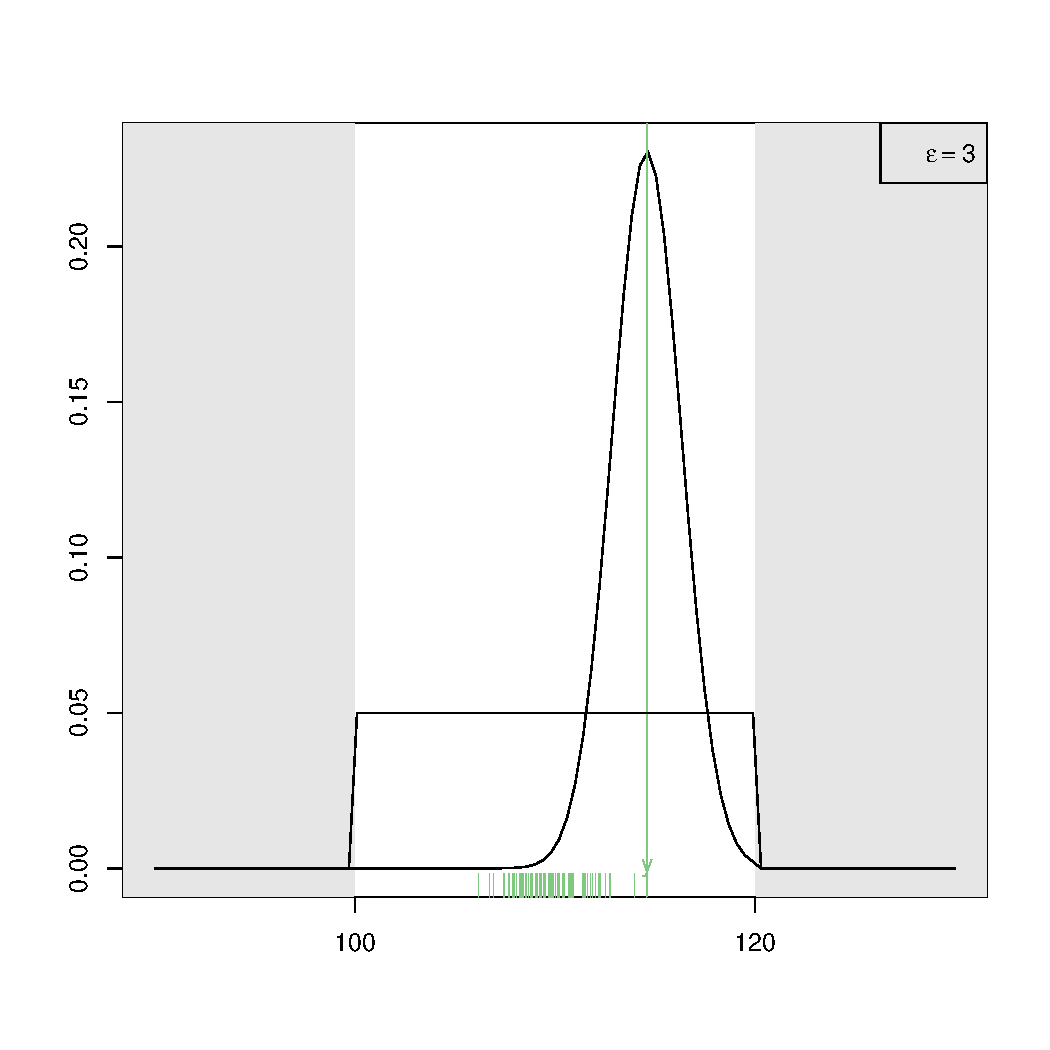
\includegraphics[scale=.35]{./Images/concentrate_0.pdf}}%
\only<2>{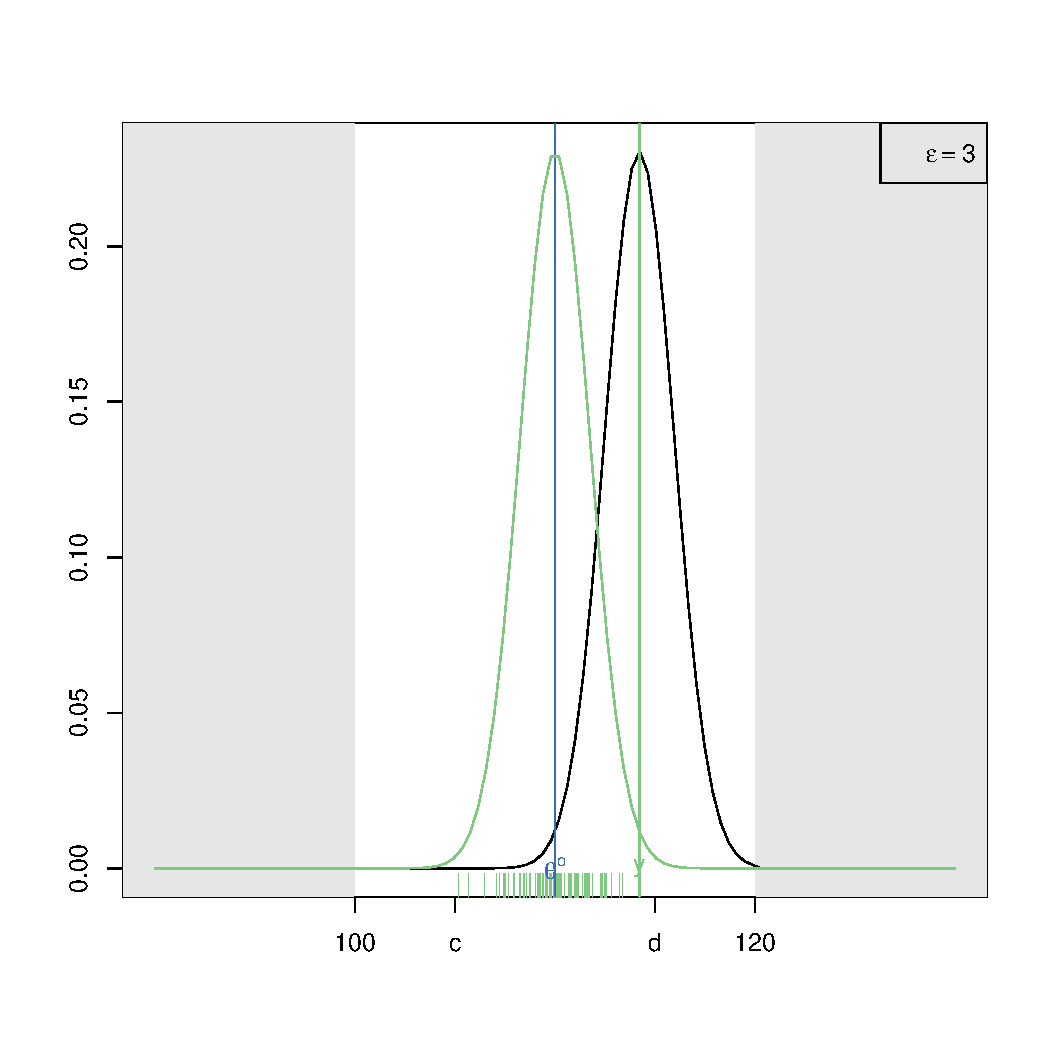
\includegraphics[scale=.35]{./Images/concentrate_1.pdf}}%
\only<3>{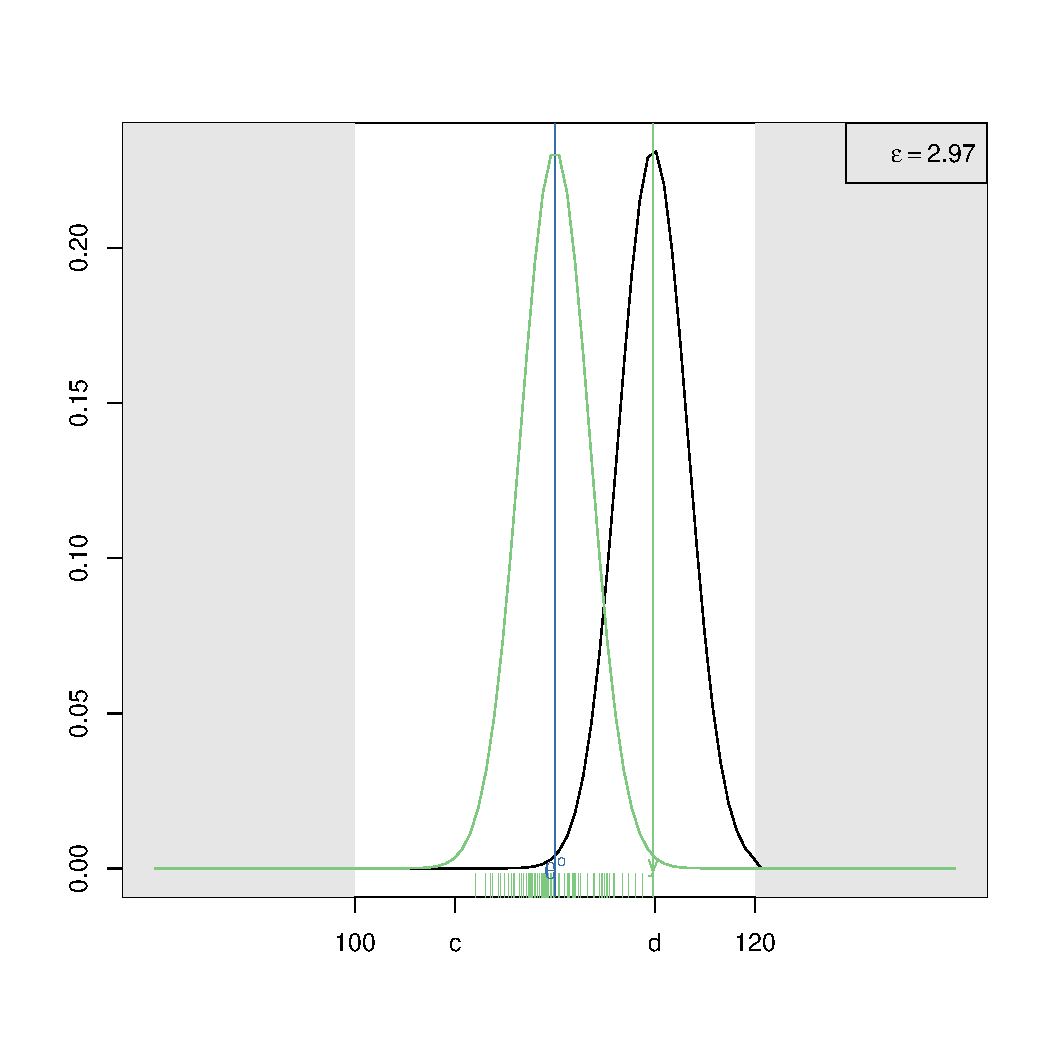
\includegraphics[scale=.35]{./Images/concentrate_2.pdf}}%
\only<4>{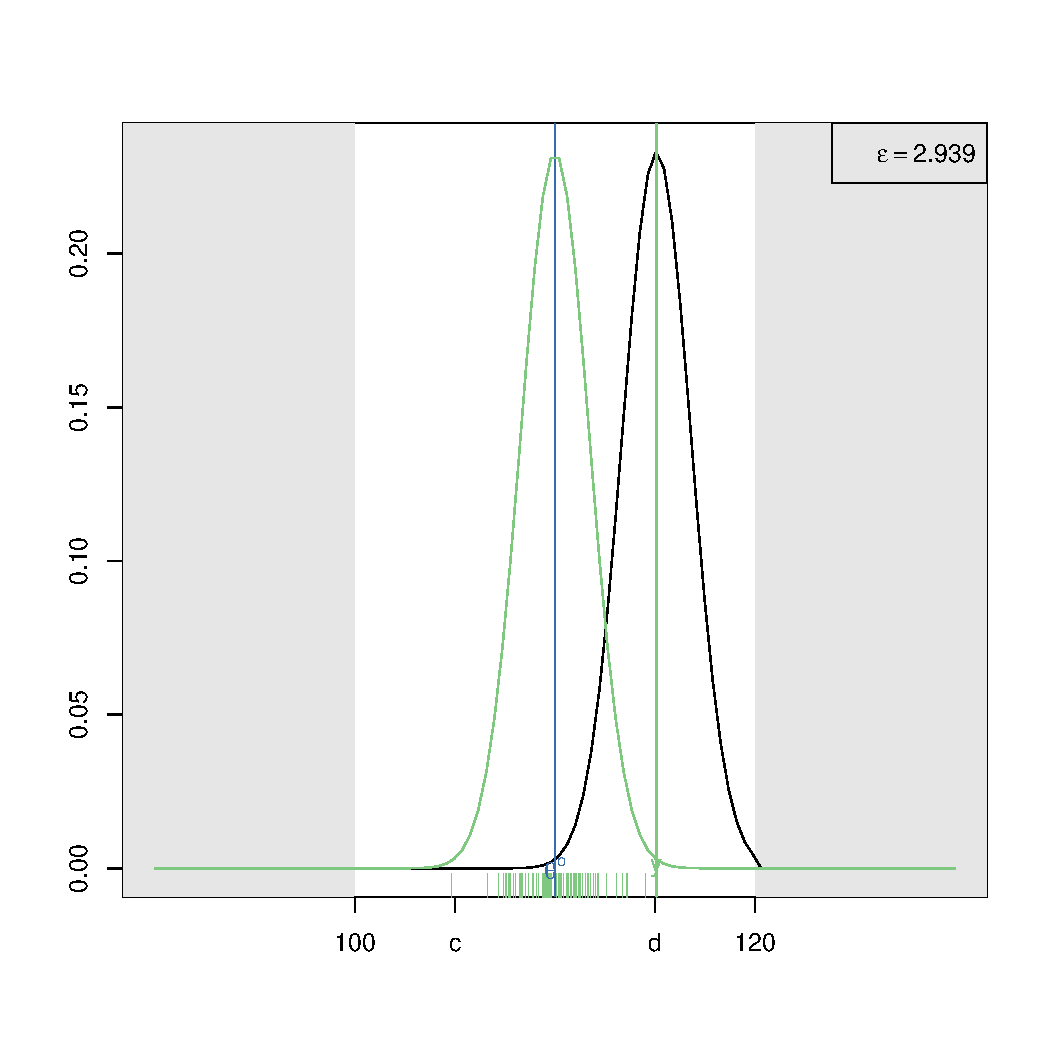
\includegraphics[scale=.35]{./Images/concentrate_3.pdf}}%
\only<5>{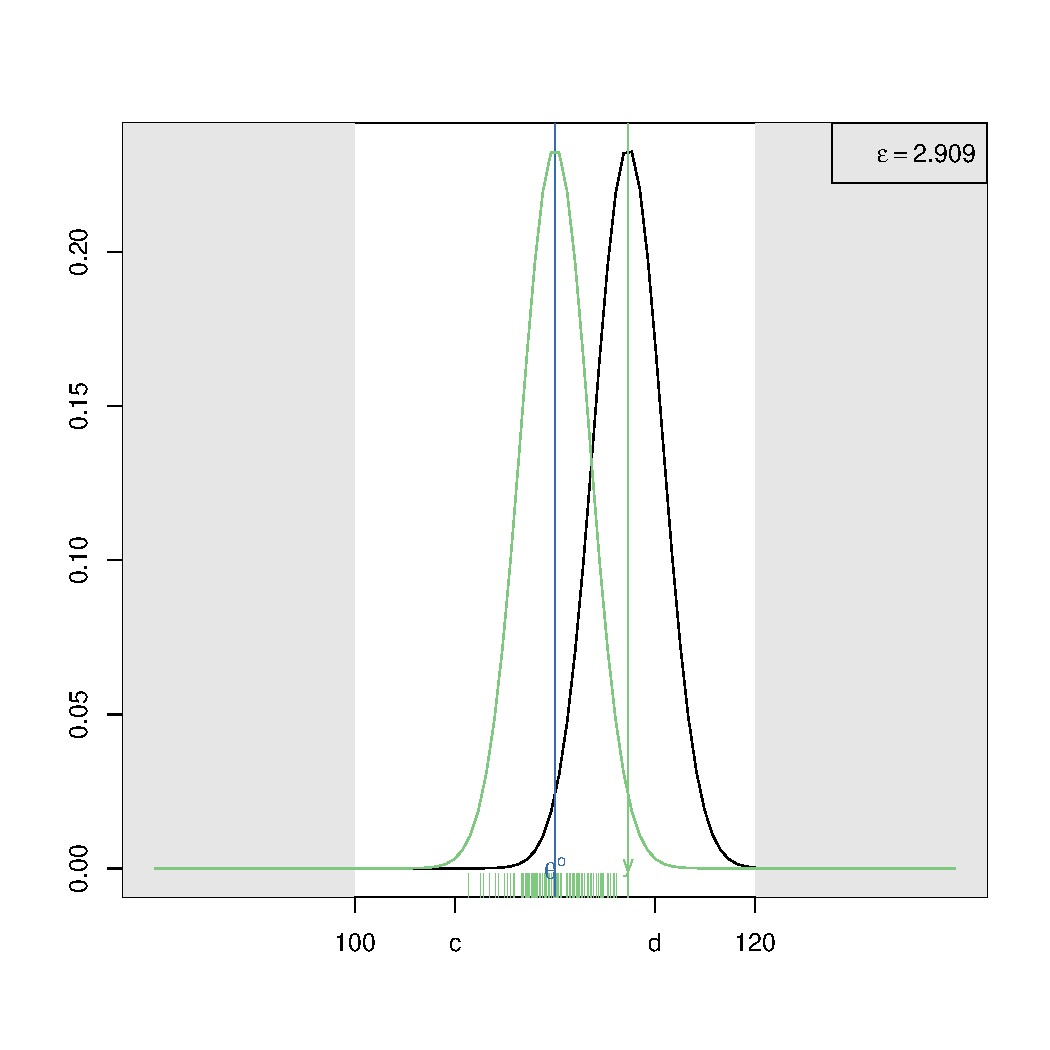
\includegraphics[scale=.35]{./Images/concentrate_4.pdf}}%
\only<6>{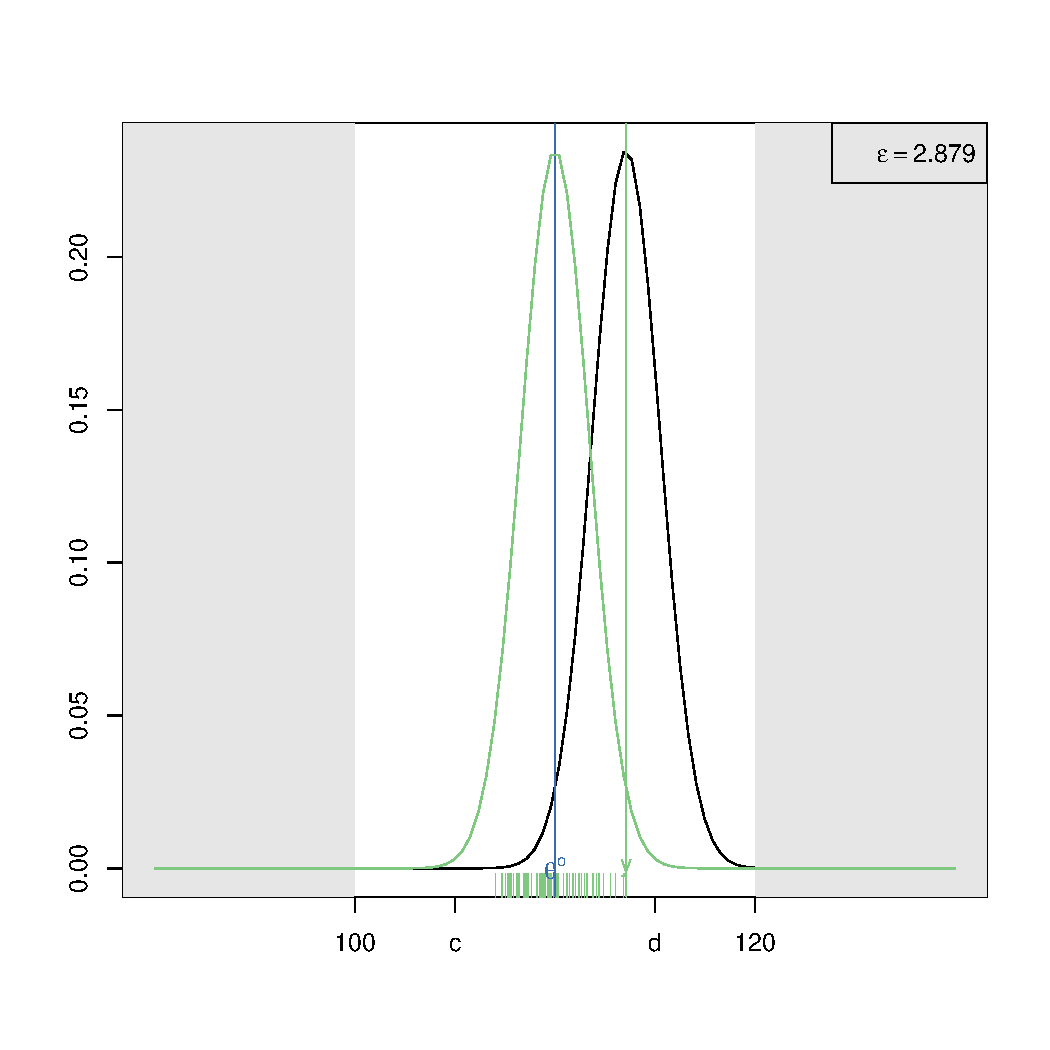
\includegraphics[scale=.35]{./Images/concentrate_5.pdf}}%
\only<7>{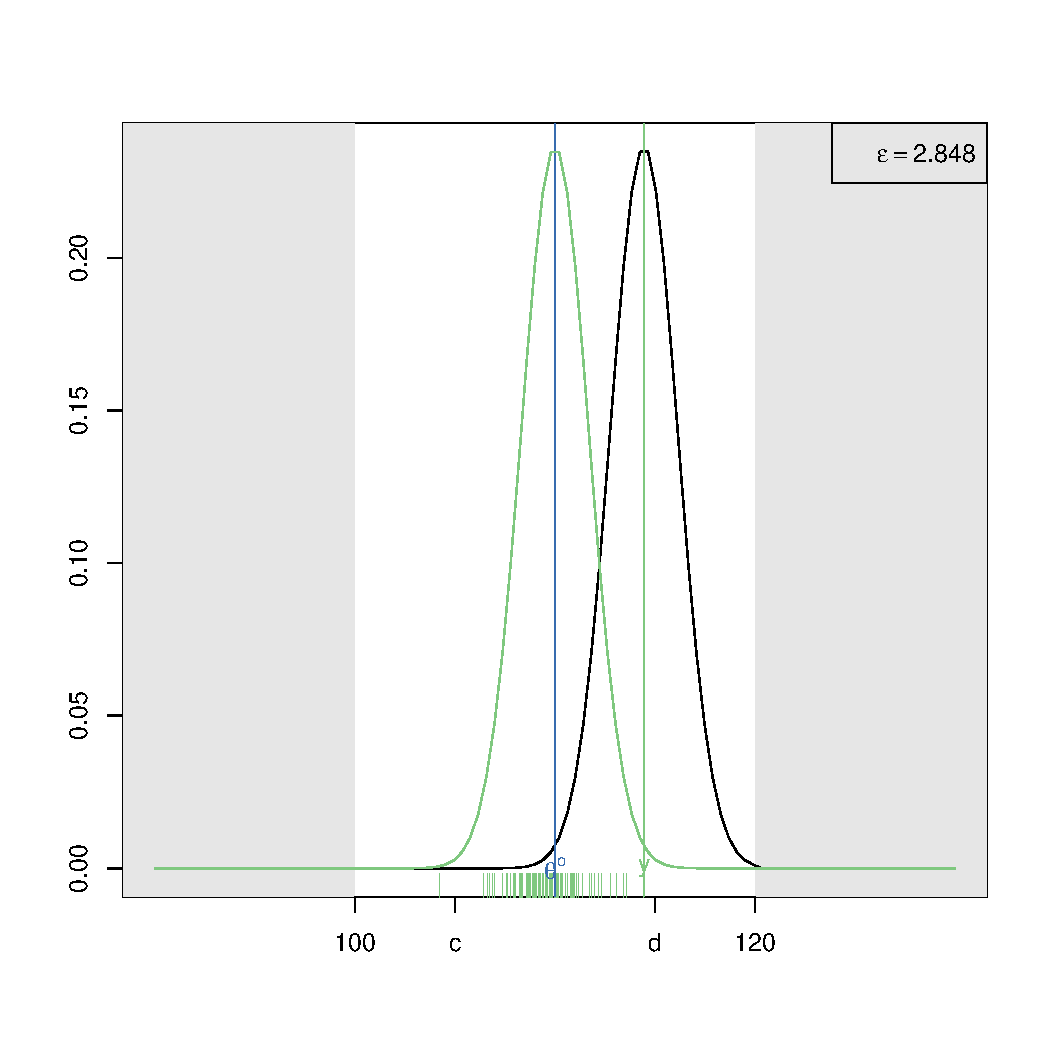
\includegraphics[scale=.35]{./Images/concentrate_6.pdf}}%
\only<8>{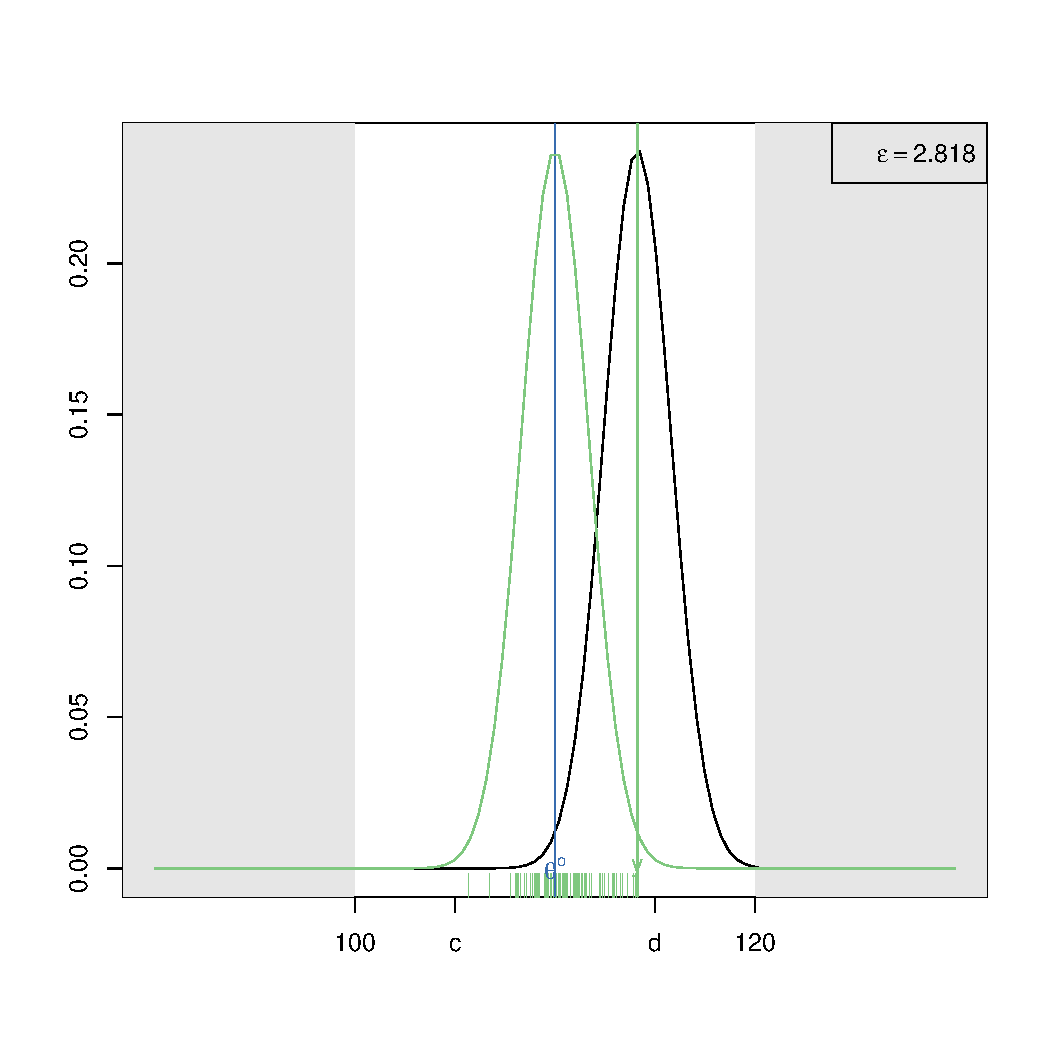
\includegraphics[scale=.35]{./Images/concentrate_7.pdf}}%
\only<9>{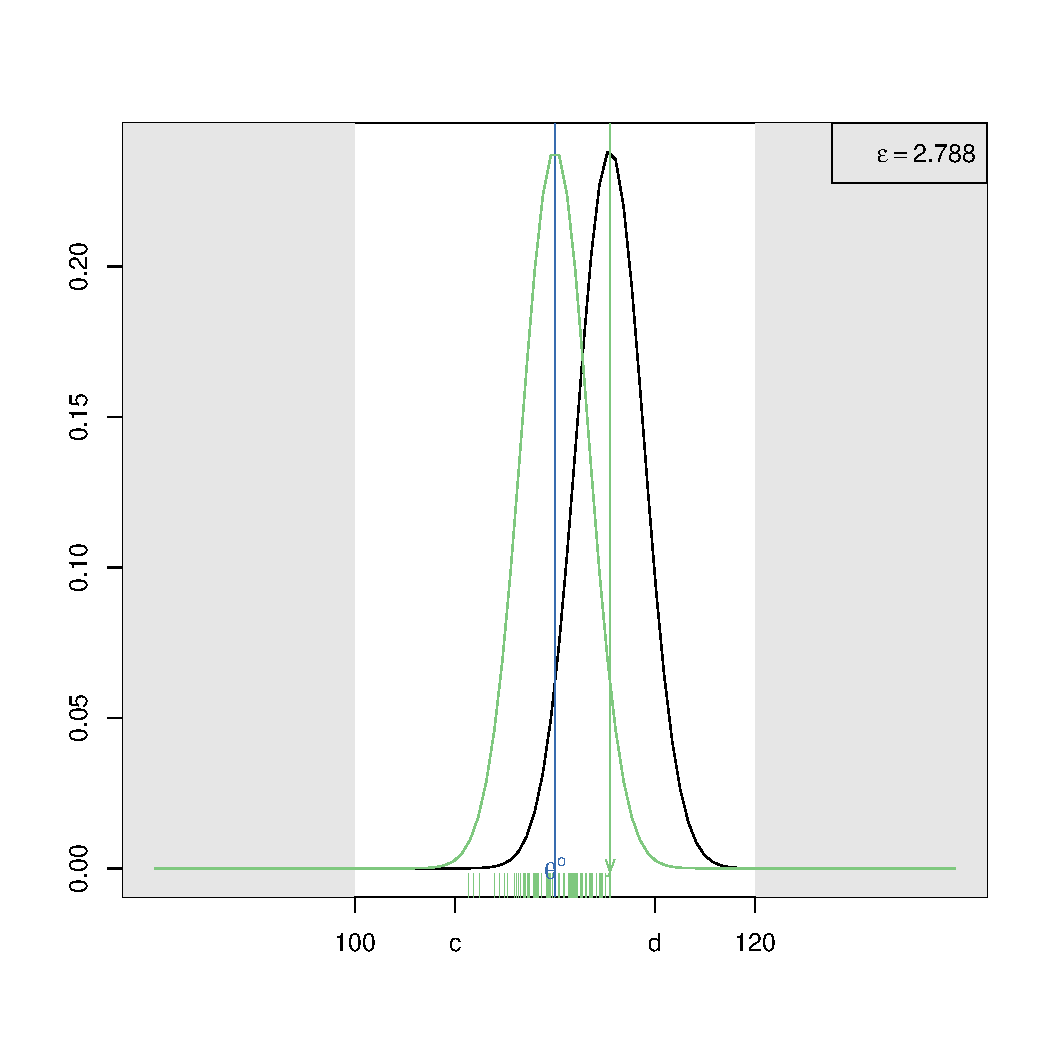
\includegraphics[scale=.35]{./Images/concentrate_8.pdf}}%
\only<10>{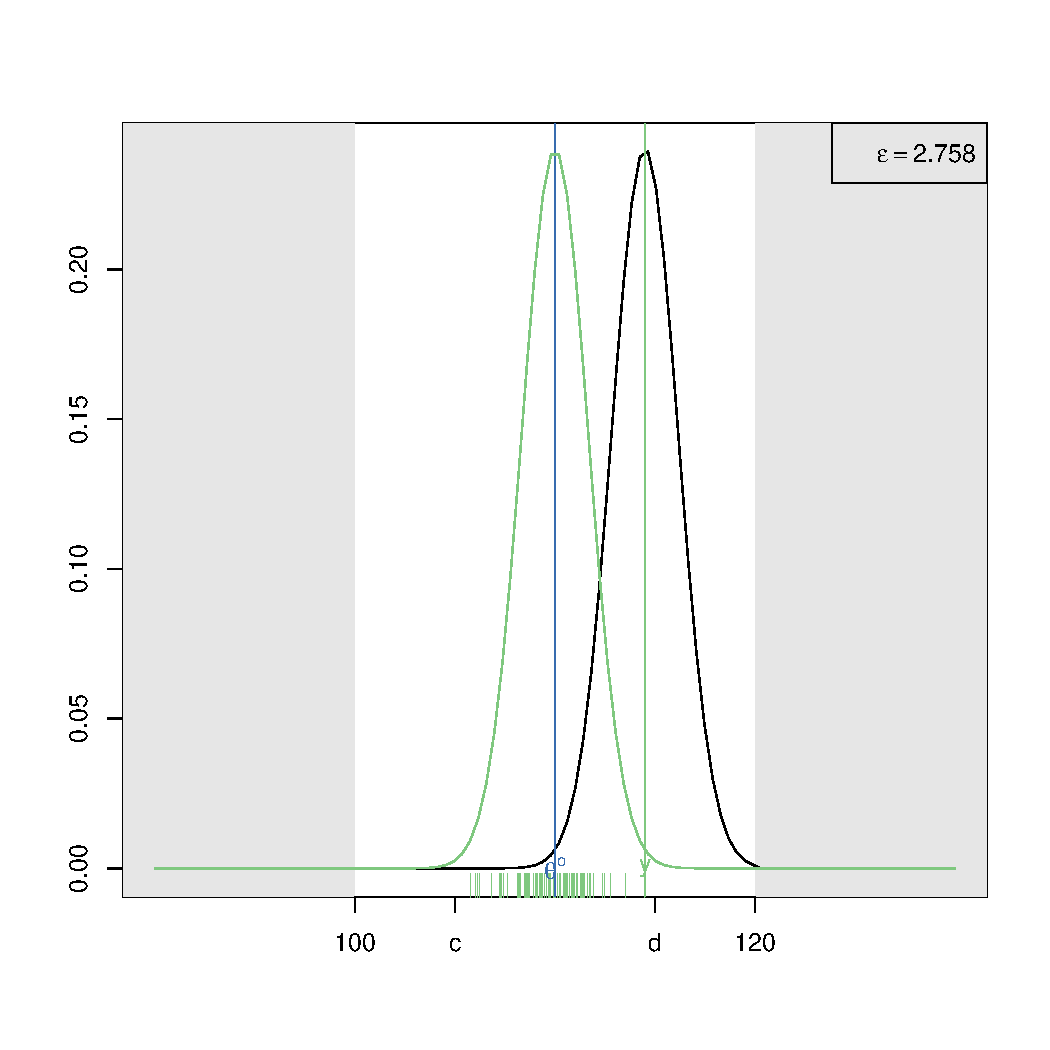
\includegraphics[scale=.35]{./Images/concentrate_9.pdf}}%
\only<11>{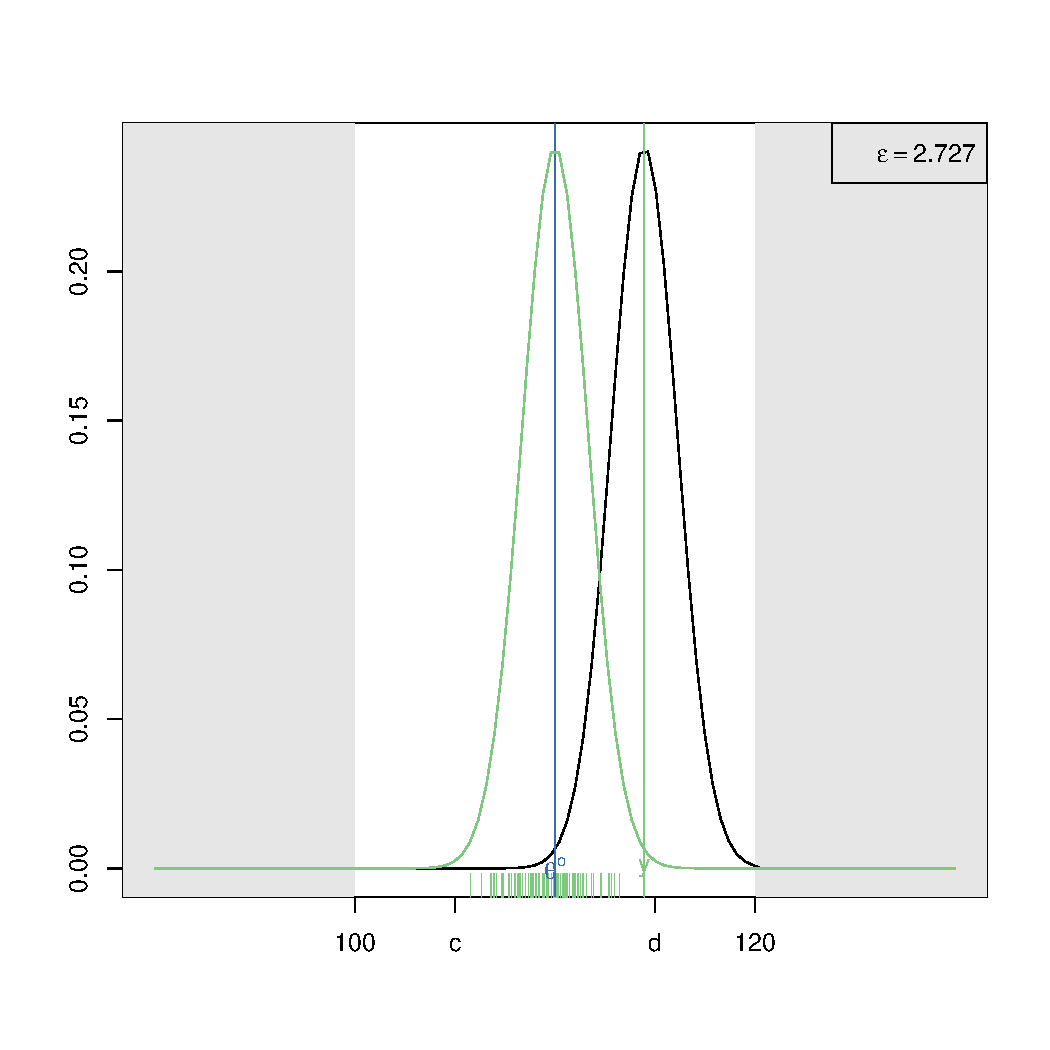
\includegraphics[scale=.35]{./Images/concentrate_10.pdf}}%
\only<12>{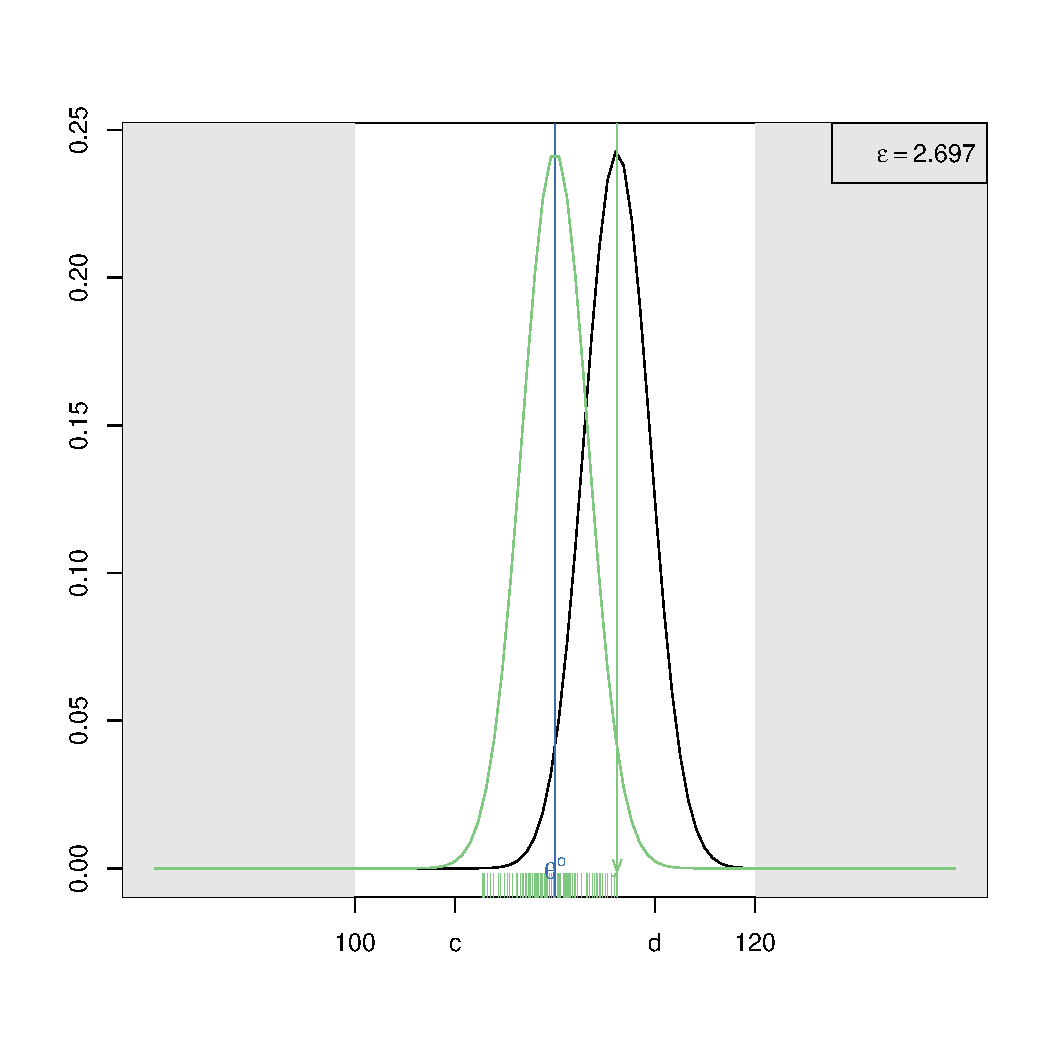
\includegraphics[scale=.35]{./Images/concentrate_11.pdf}}%
\only<13>{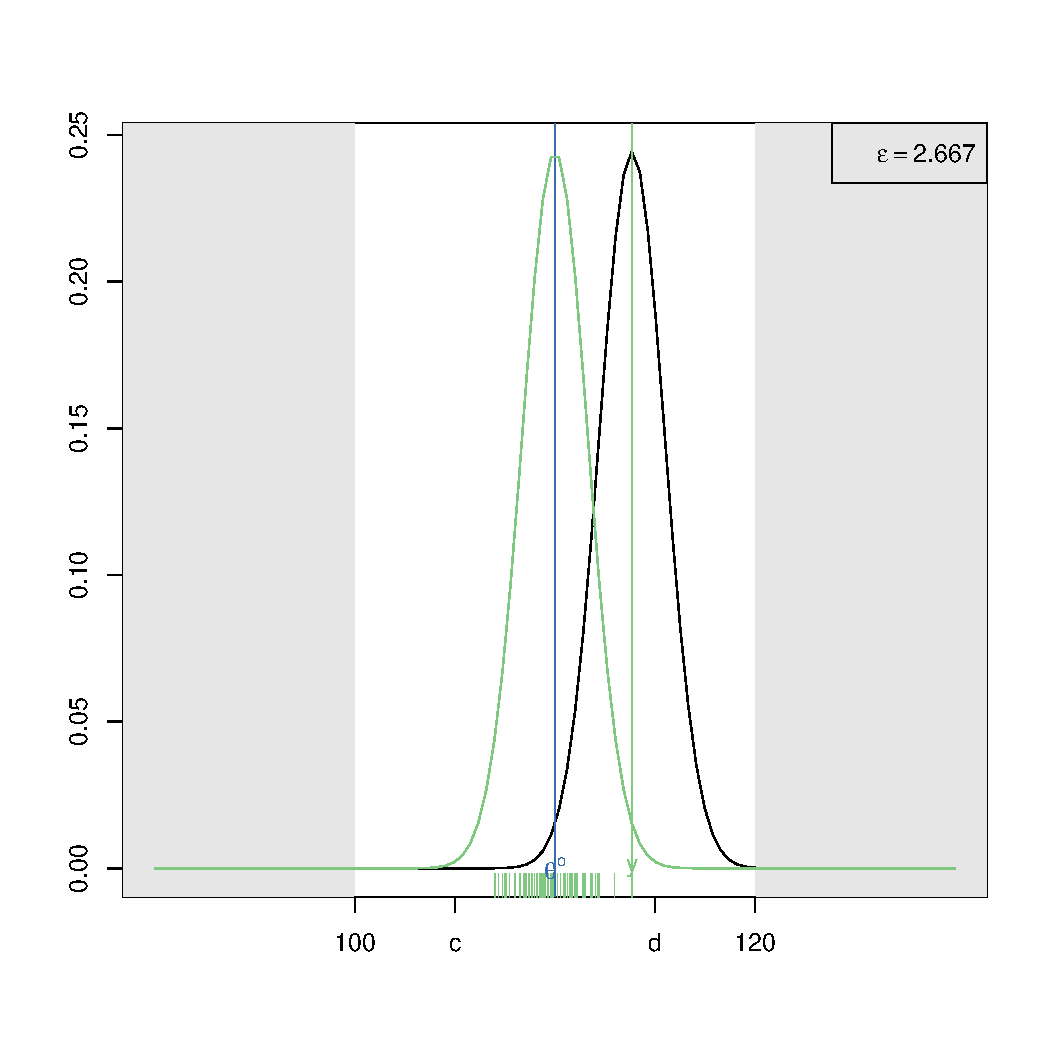
\includegraphics[scale=.35]{./Images/concentrate_12.pdf}}%
\only<14>{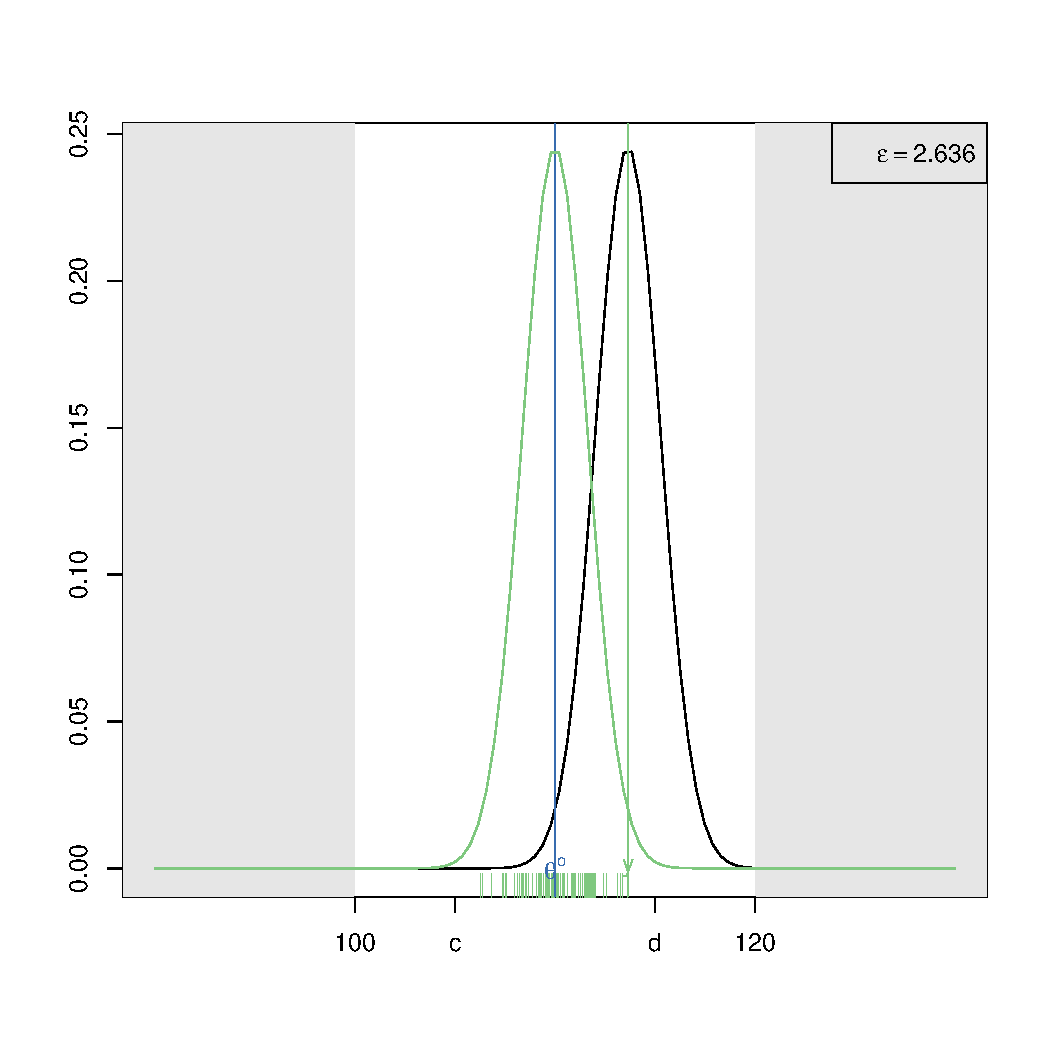
\includegraphics[scale=.35]{./Images/concentrate_13.pdf}}%
\only<15>{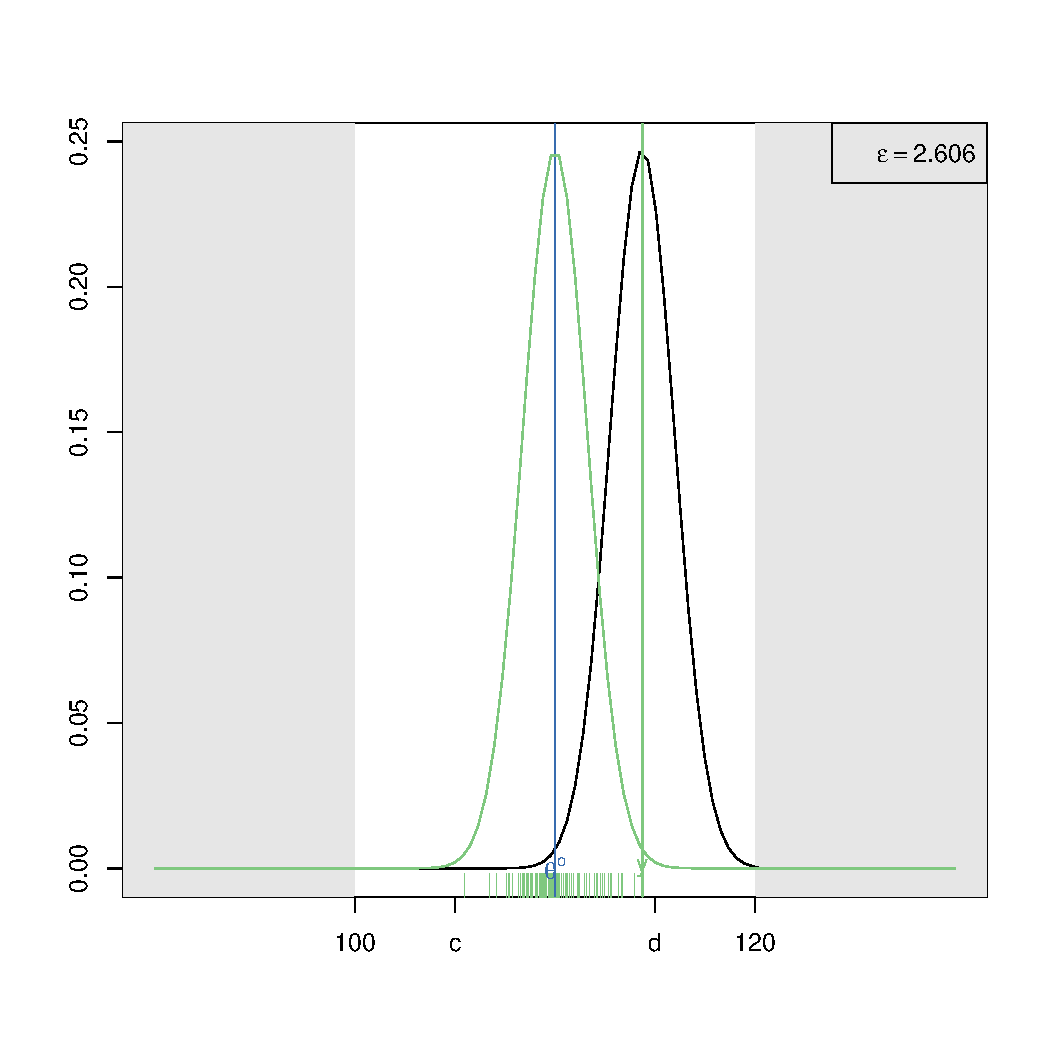
\includegraphics[scale=.35]{./Images/concentrate_14.pdf}}%
\only<16>{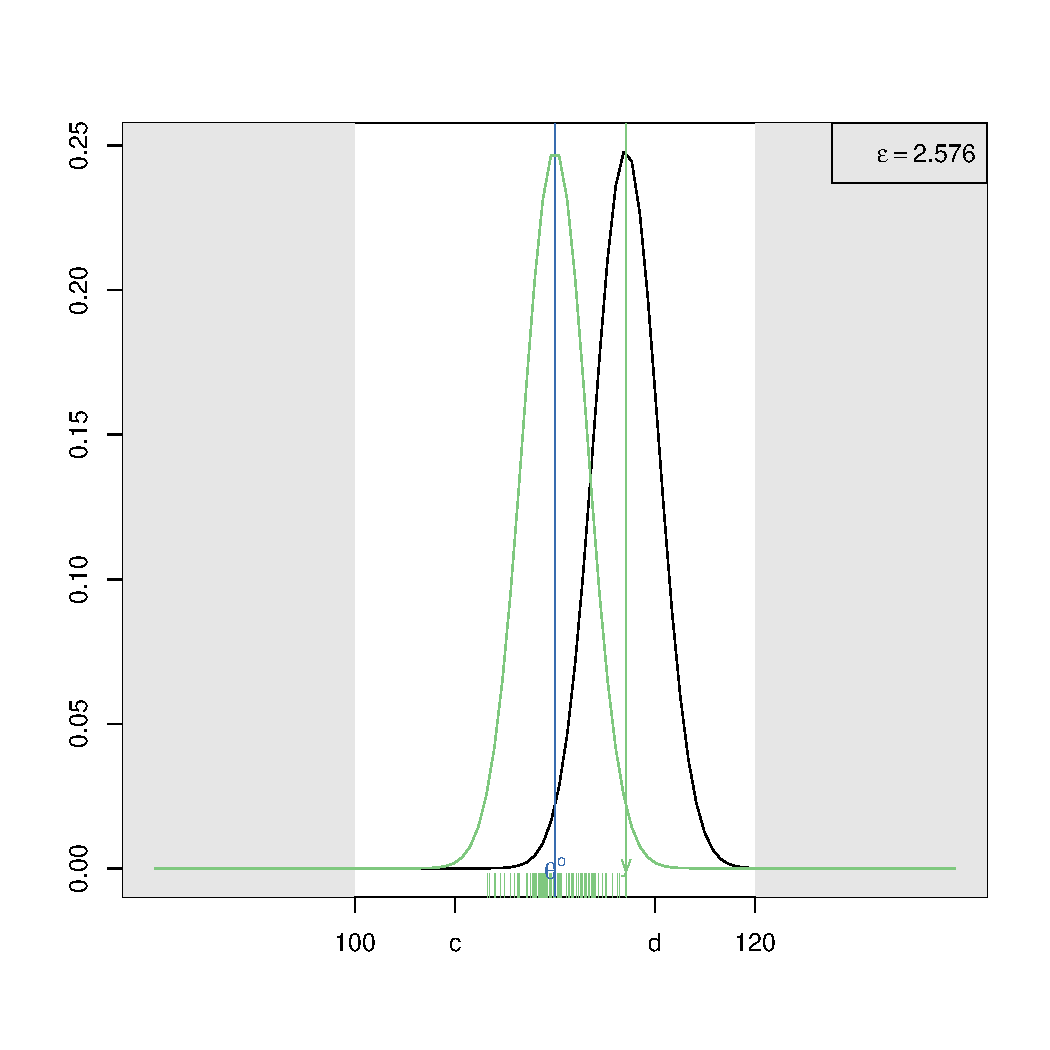
\includegraphics[scale=.35]{./Images/concentrate_15.pdf}}%
\only<17>{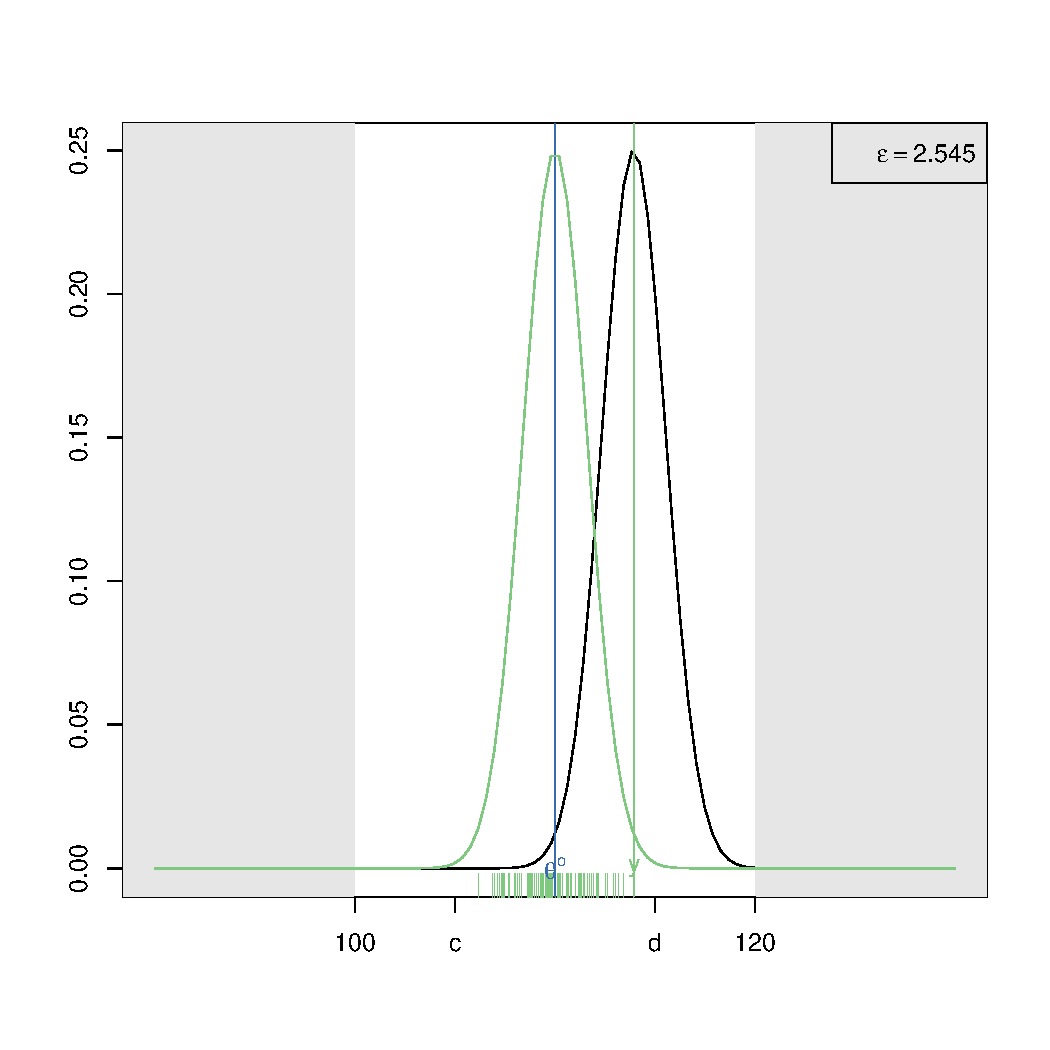
\includegraphics[scale=.35]{./Images/concentrate_16.pdf}}%
\only<18>{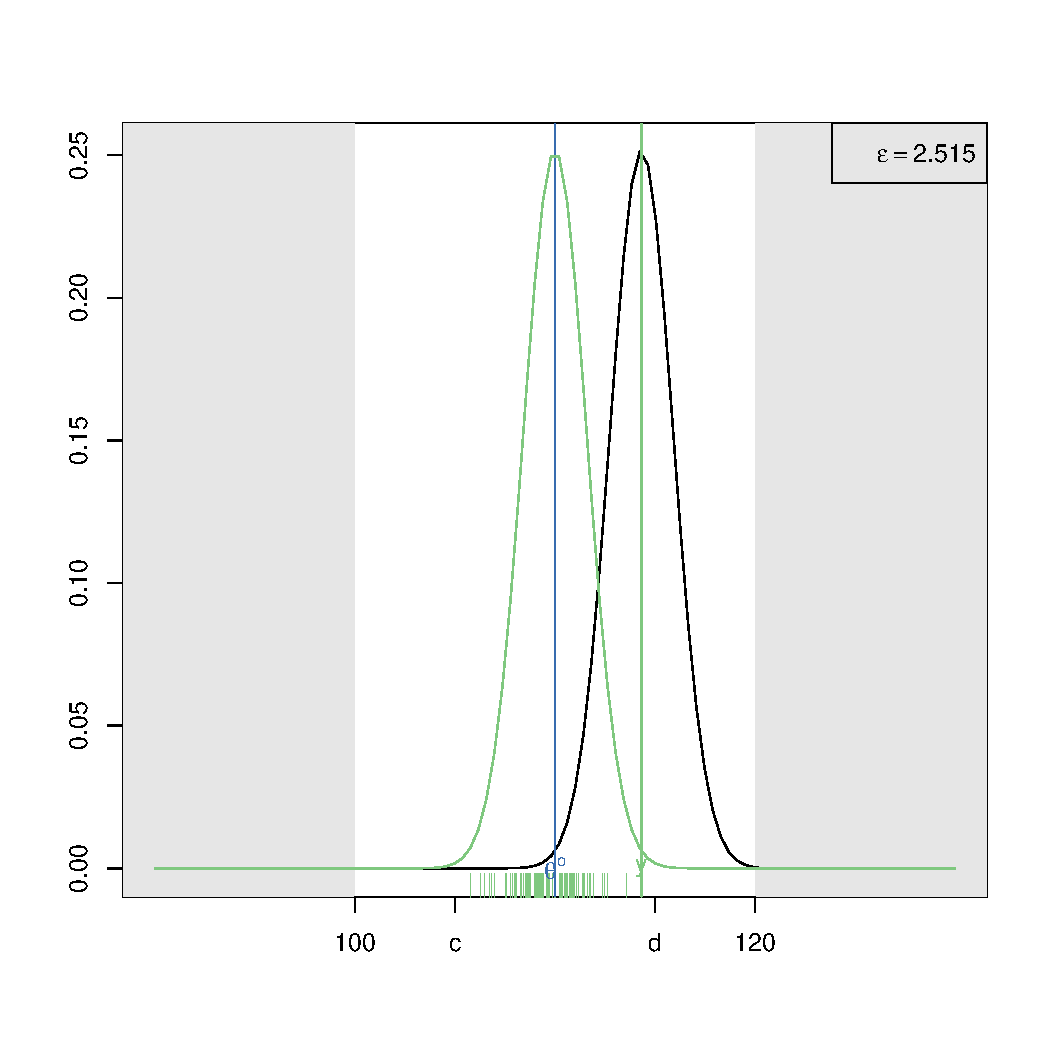
\includegraphics[scale=.35]{./Images/concentrate_17.pdf}}%
\only<19>{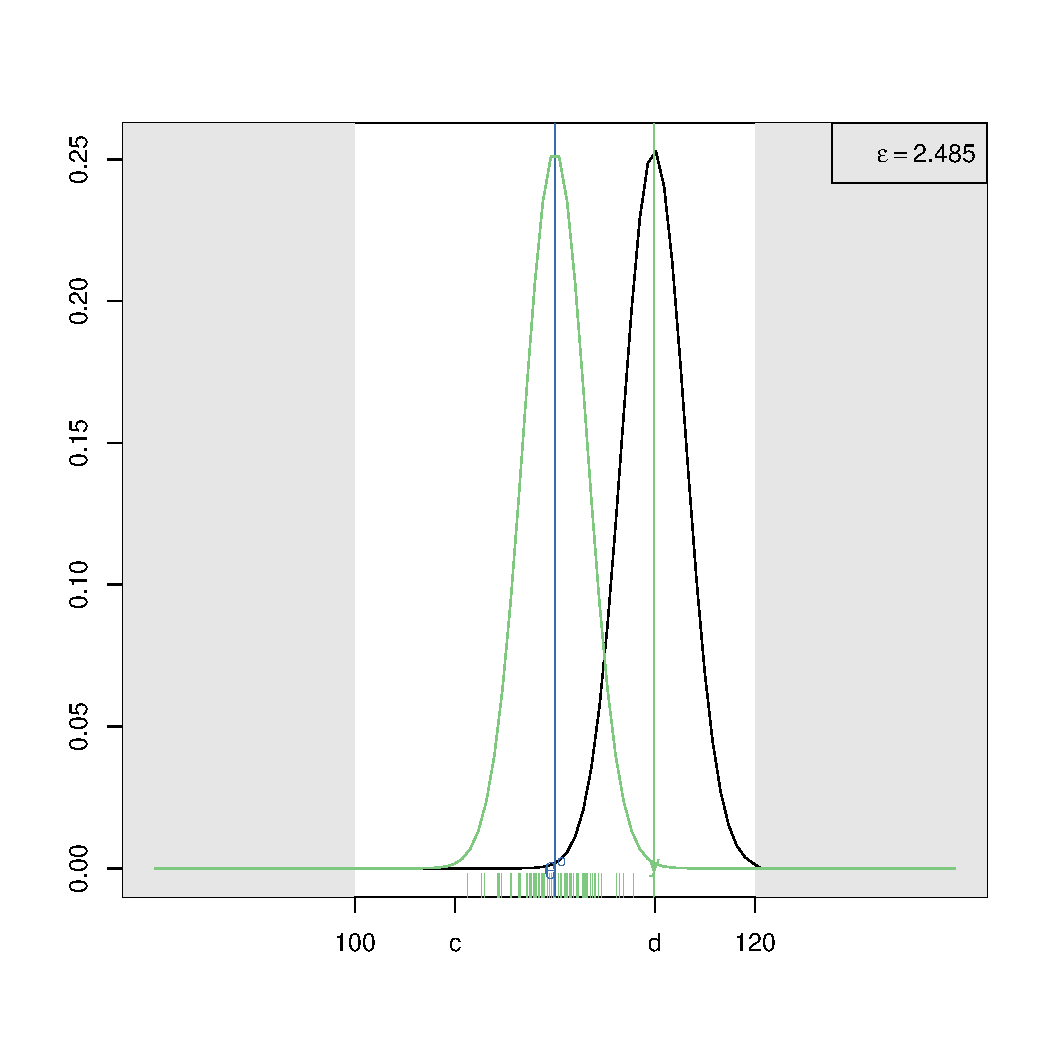
\includegraphics[scale=.35]{./Images/concentrate_18.pdf}}%
\only<20>{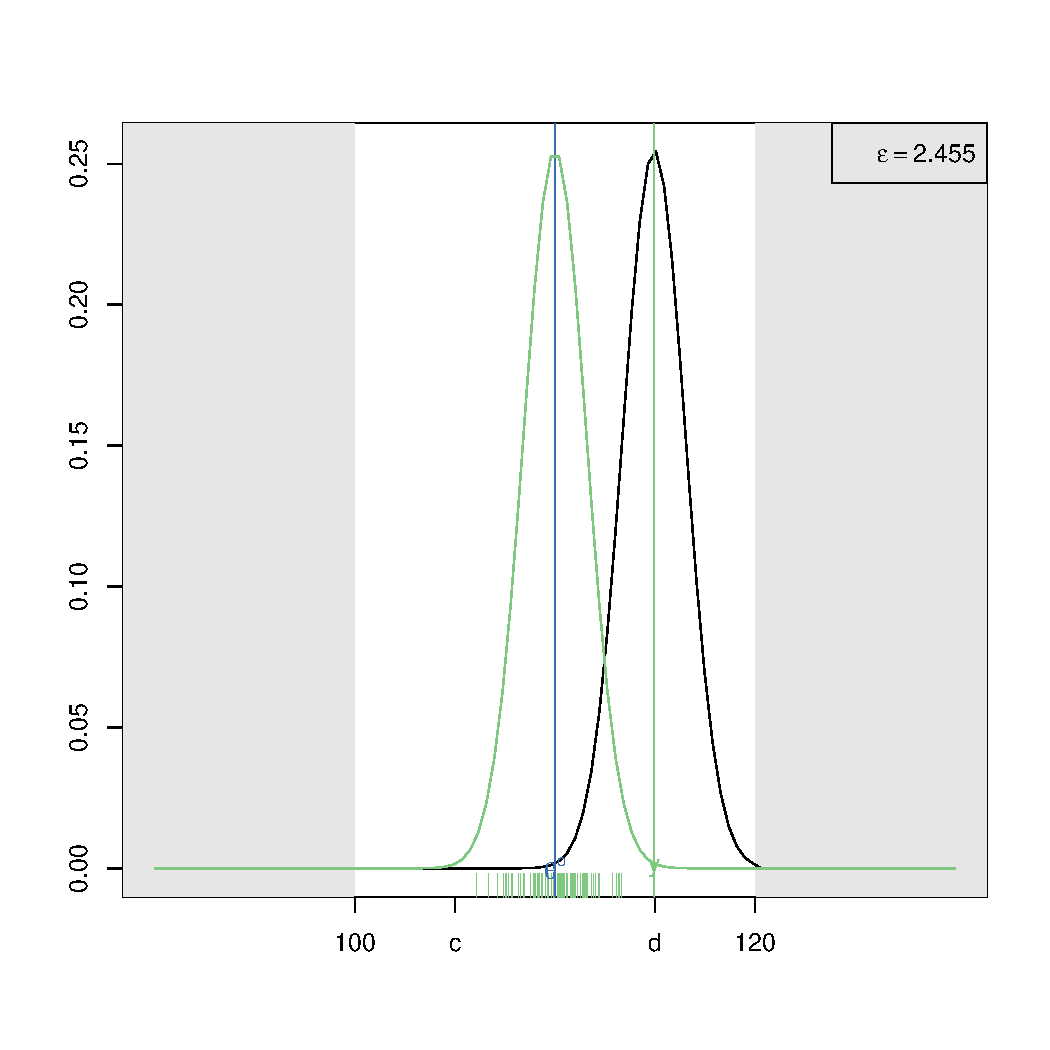
\includegraphics[scale=.35]{./Images/concentrate_19.pdf}}%
\only<21>{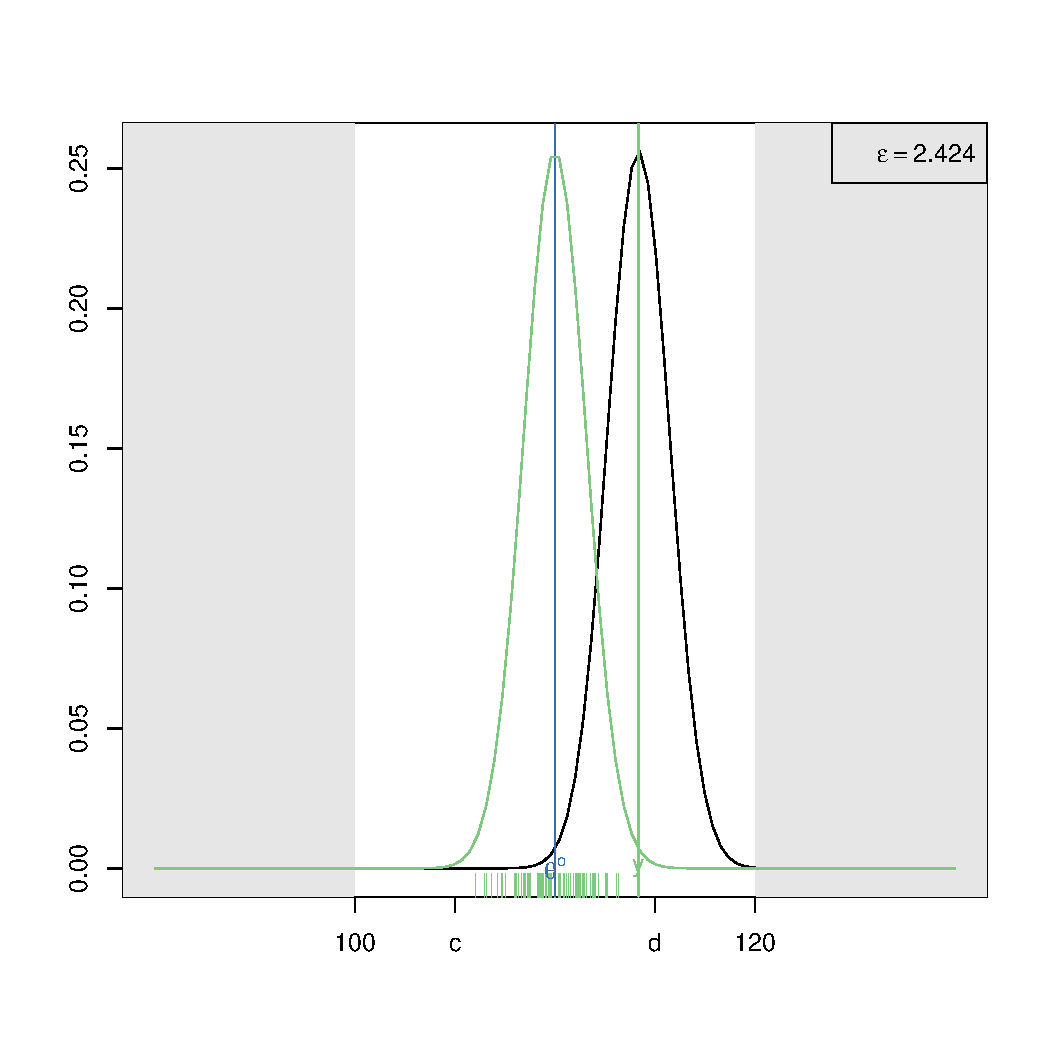
\includegraphics[scale=.35]{./Images/concentrate_20.pdf}}%
\only<22>{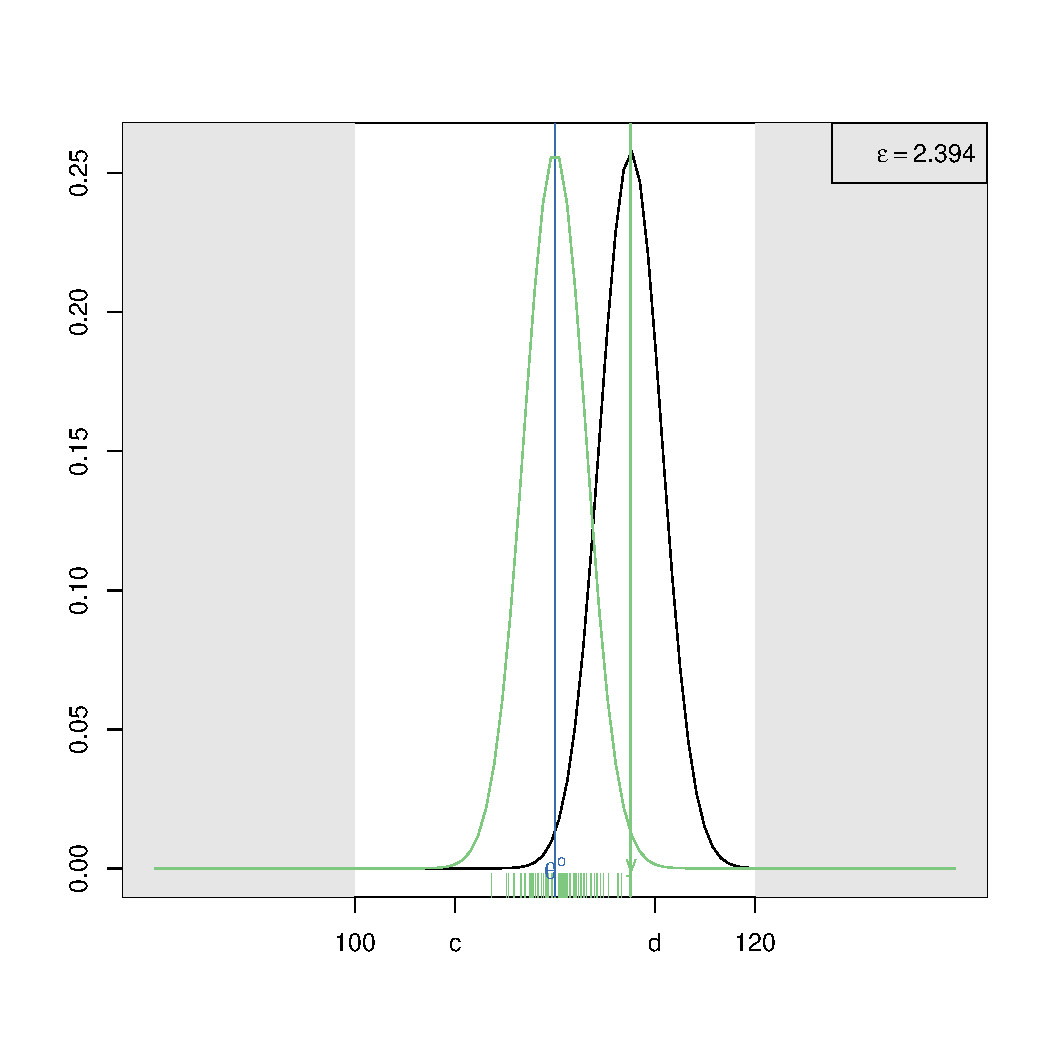
\includegraphics[scale=.35]{./Images/concentrate_21.pdf}}%
\only<23>{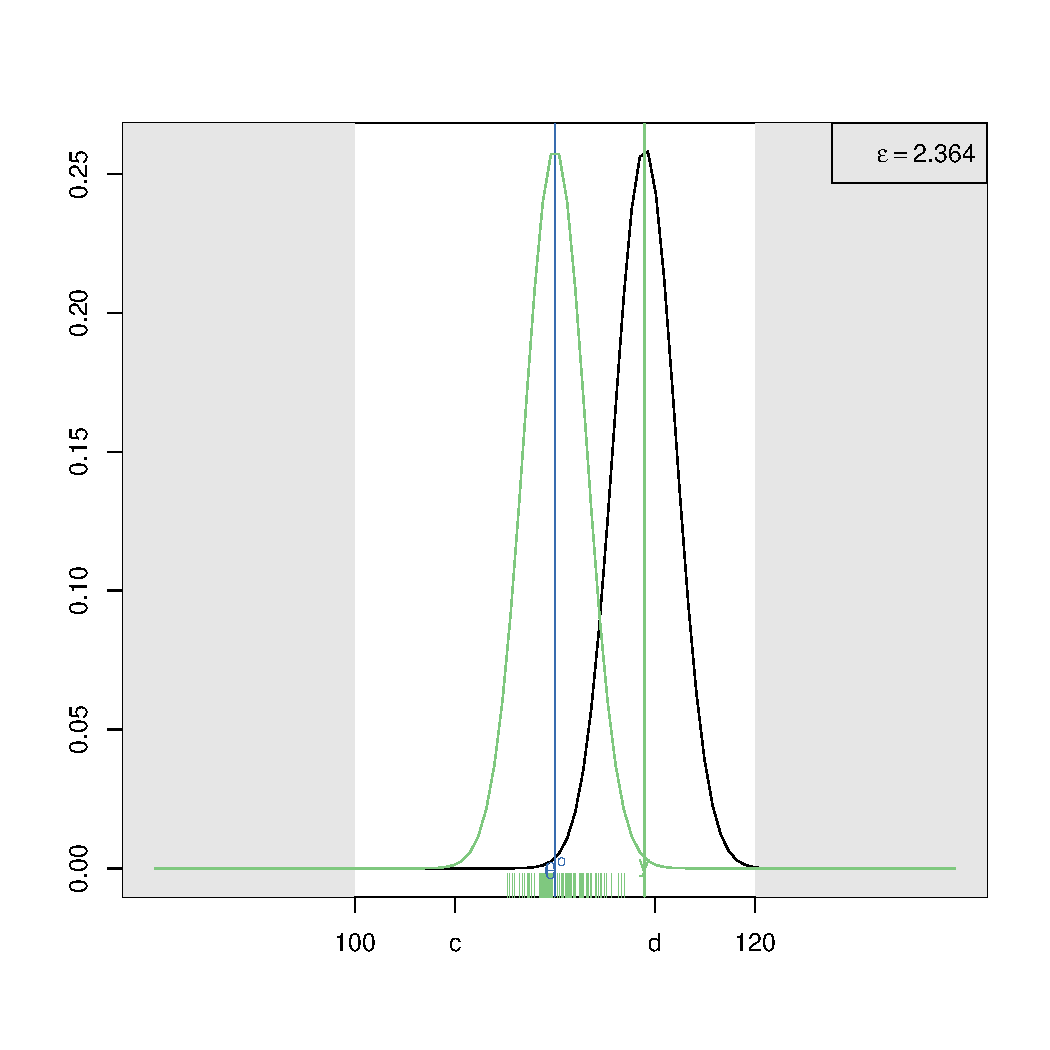
\includegraphics[scale=.35]{./Images/concentrate_22.pdf}}%
\only<24>{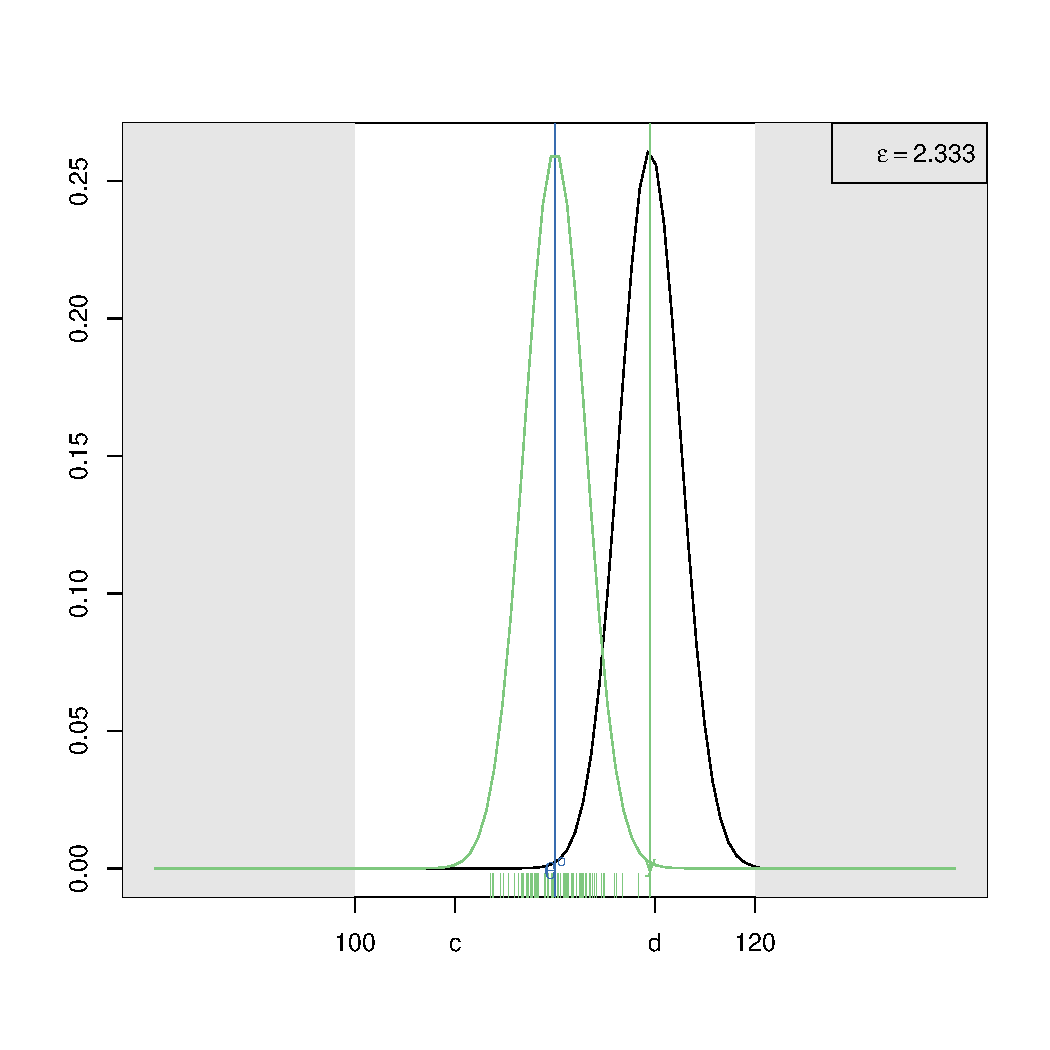
\includegraphics[scale=.35]{./Images/concentrate_23.pdf}}%
\only<25>{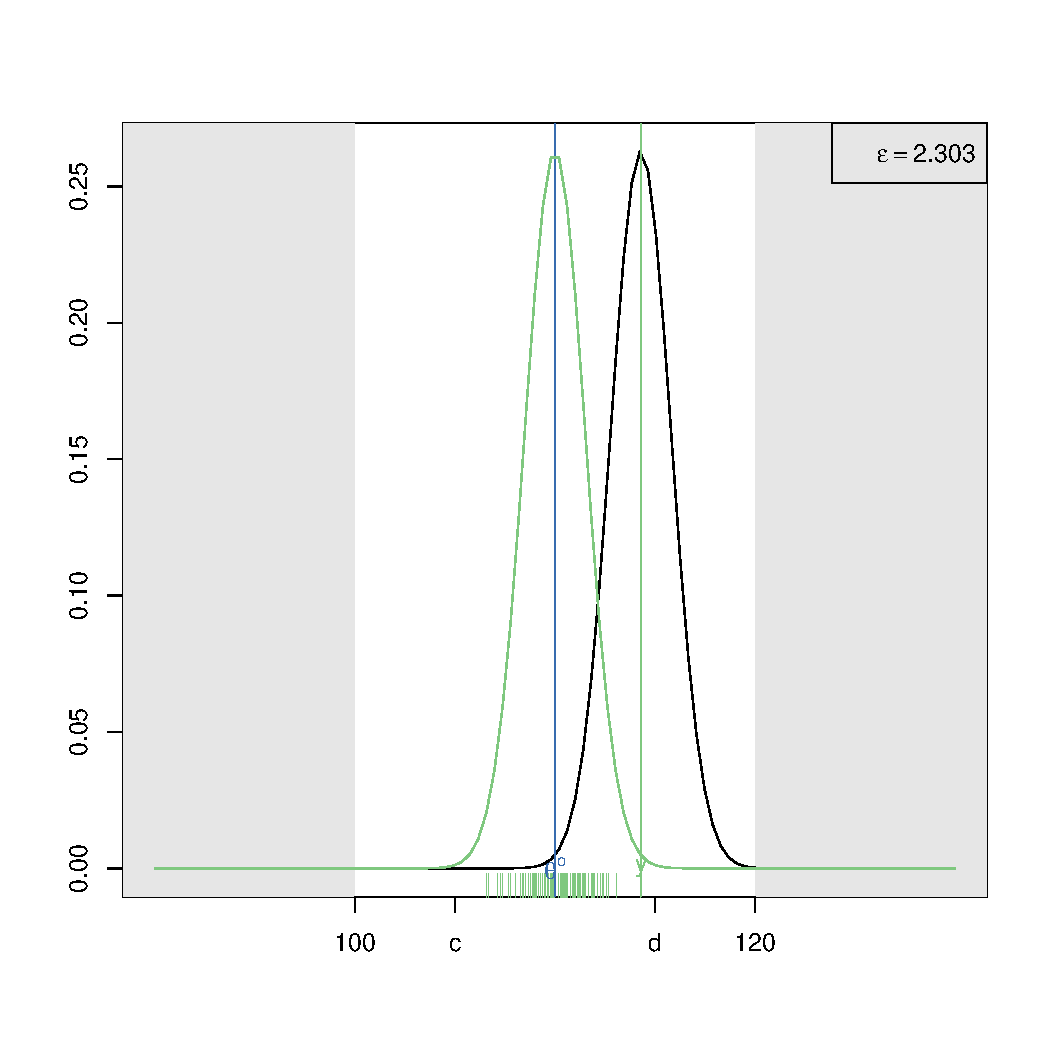
\includegraphics[scale=.35]{./Images/concentrate_24.pdf}}%
\only<26>{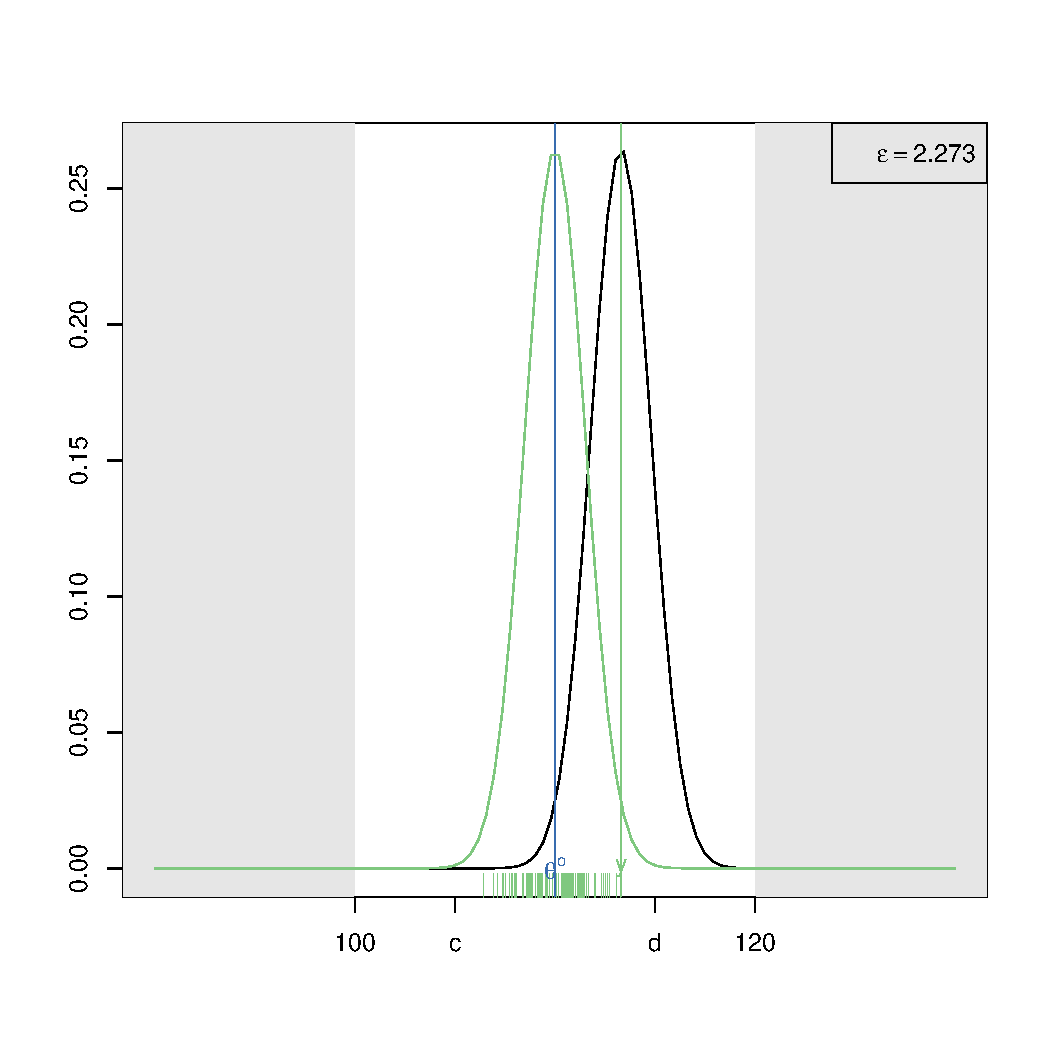
\includegraphics[scale=.35]{./Images/concentrate_25.pdf}}%
\only<27>{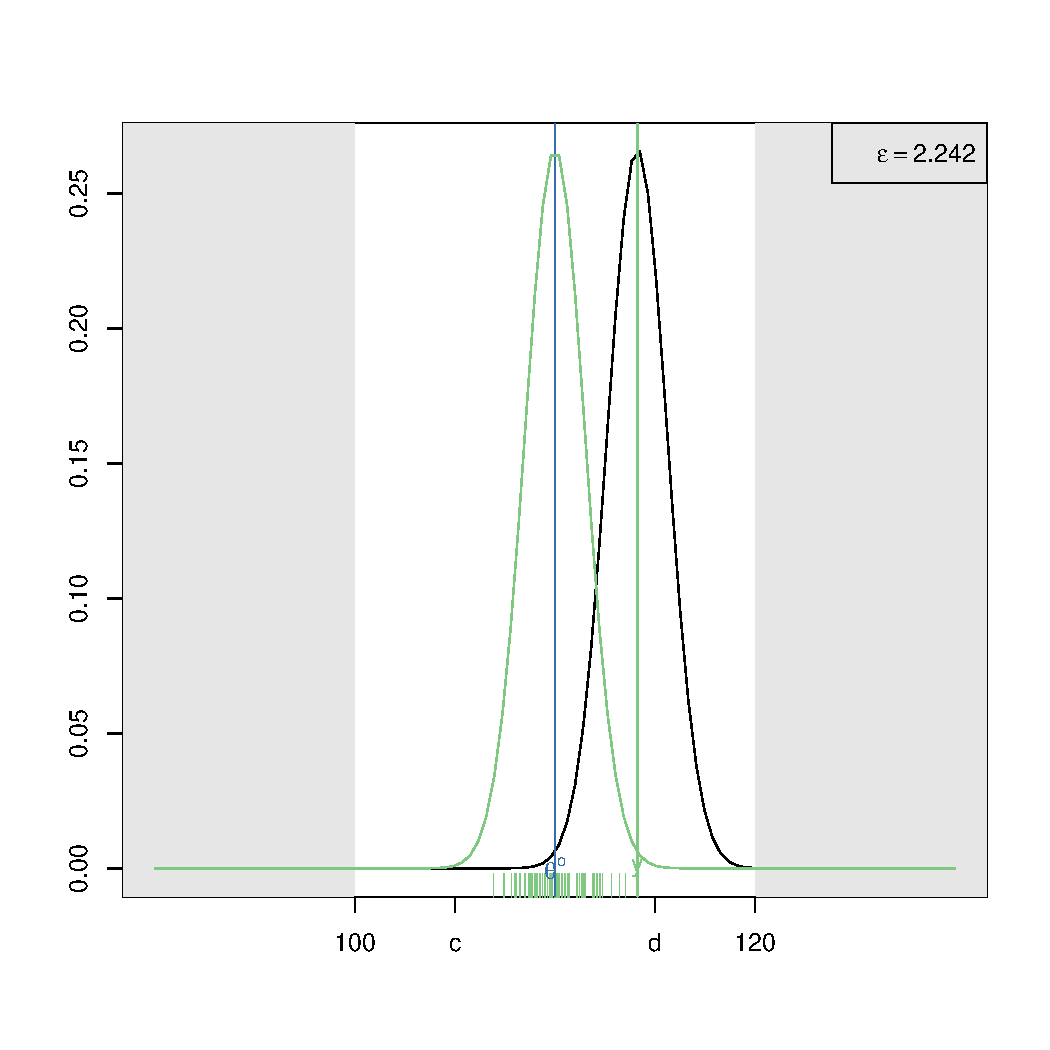
\includegraphics[scale=.35]{./Images/concentrate_26.pdf}}%
\only<28>{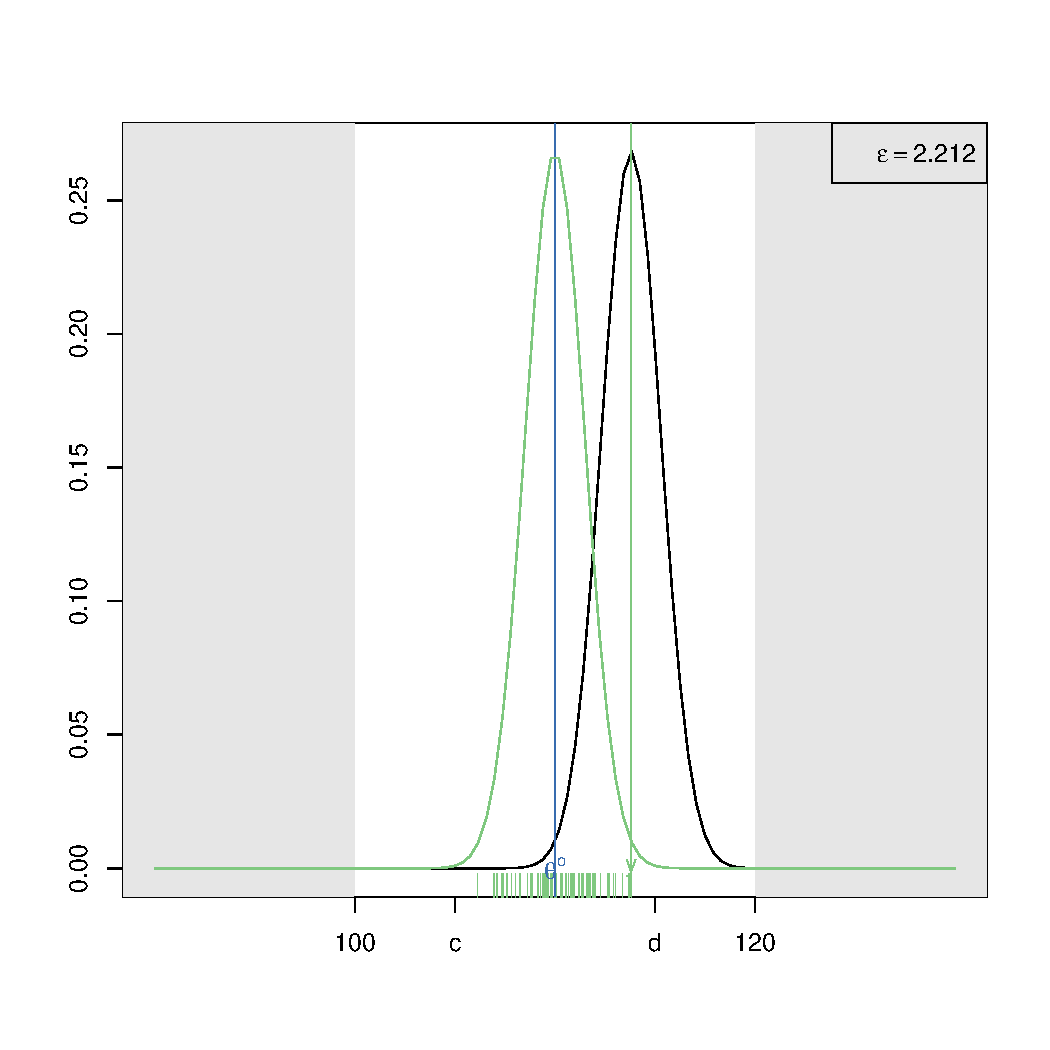
\includegraphics[scale=.35]{./Images/concentrate_27.pdf}}%
\only<29>{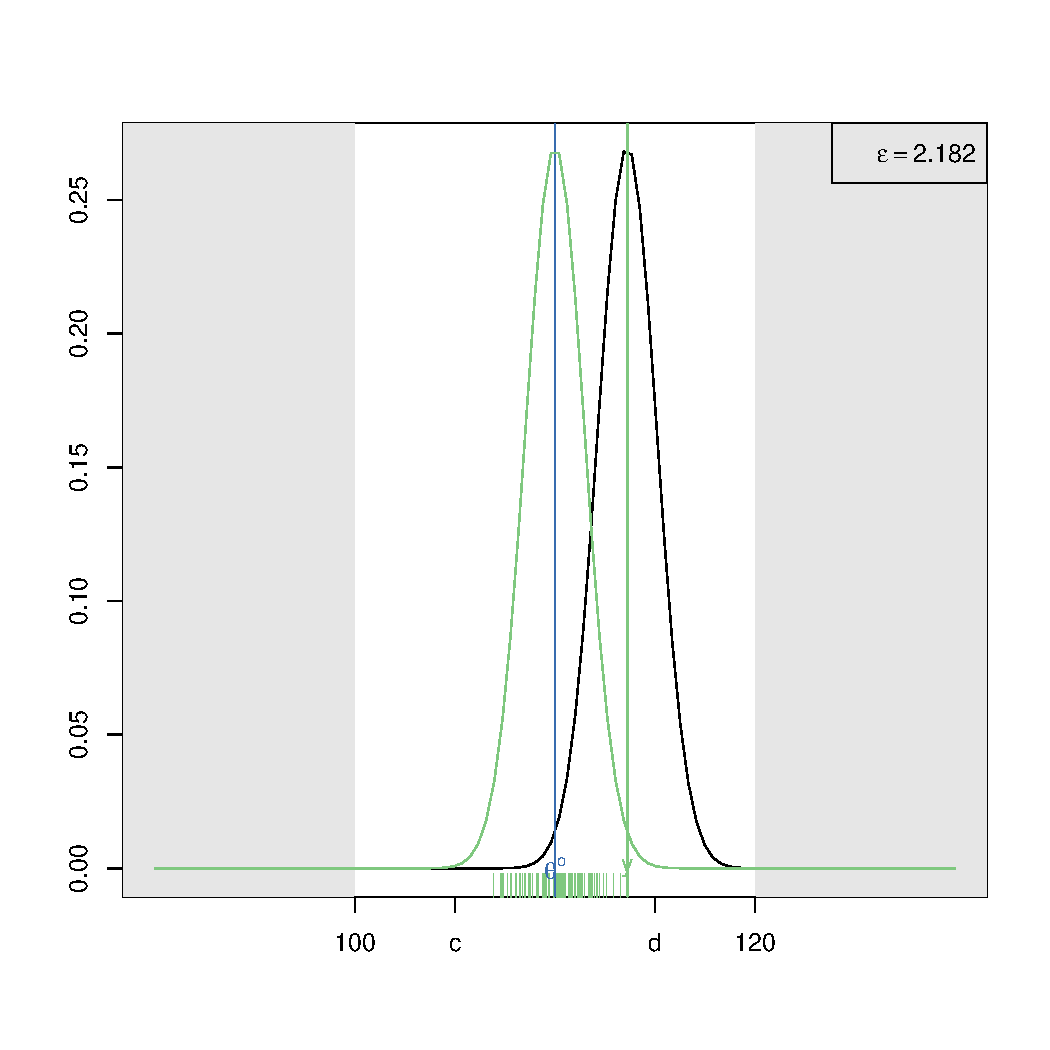
\includegraphics[scale=.35]{./Images/concentrate_28.pdf}}%
\only<30>{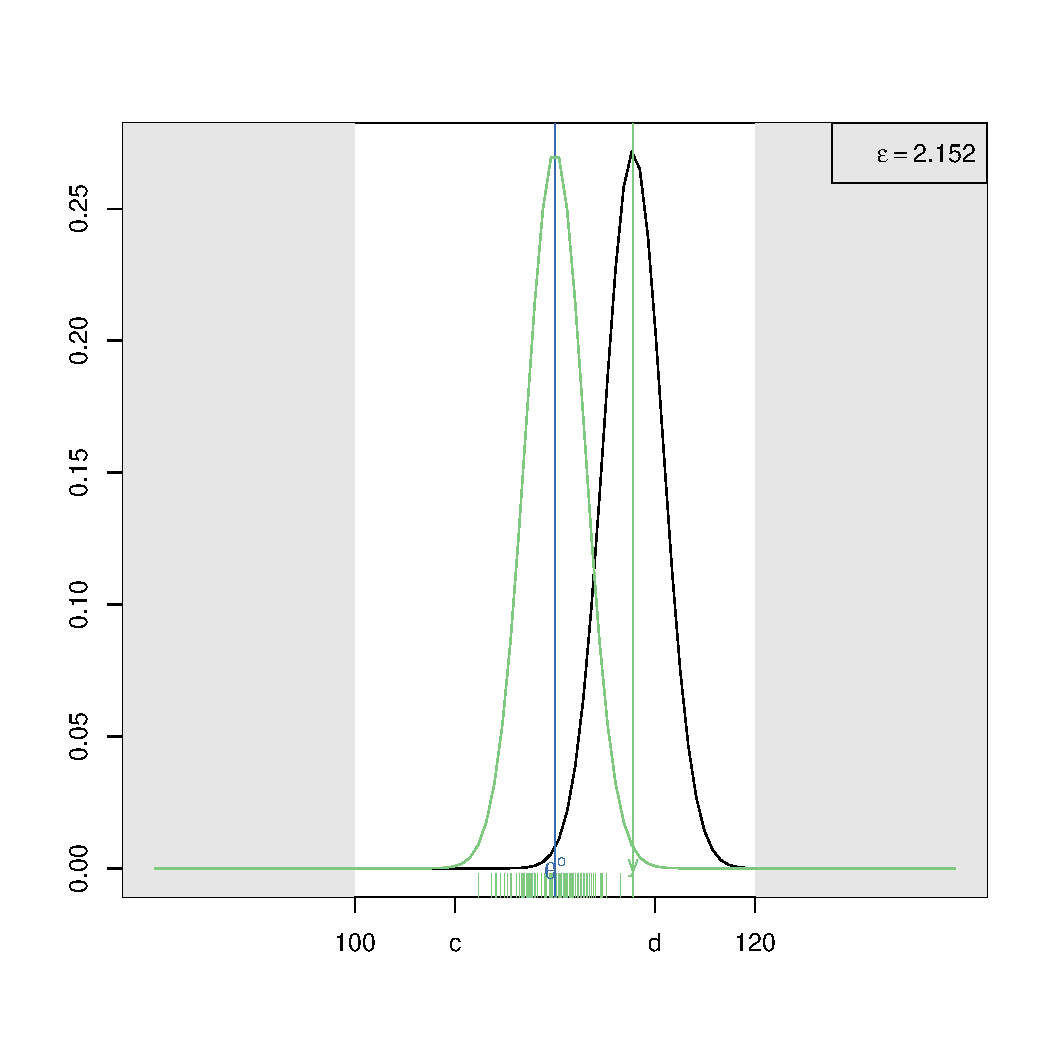
\includegraphics[scale=.35]{./Images/concentrate_29.pdf}}%
\only<31>{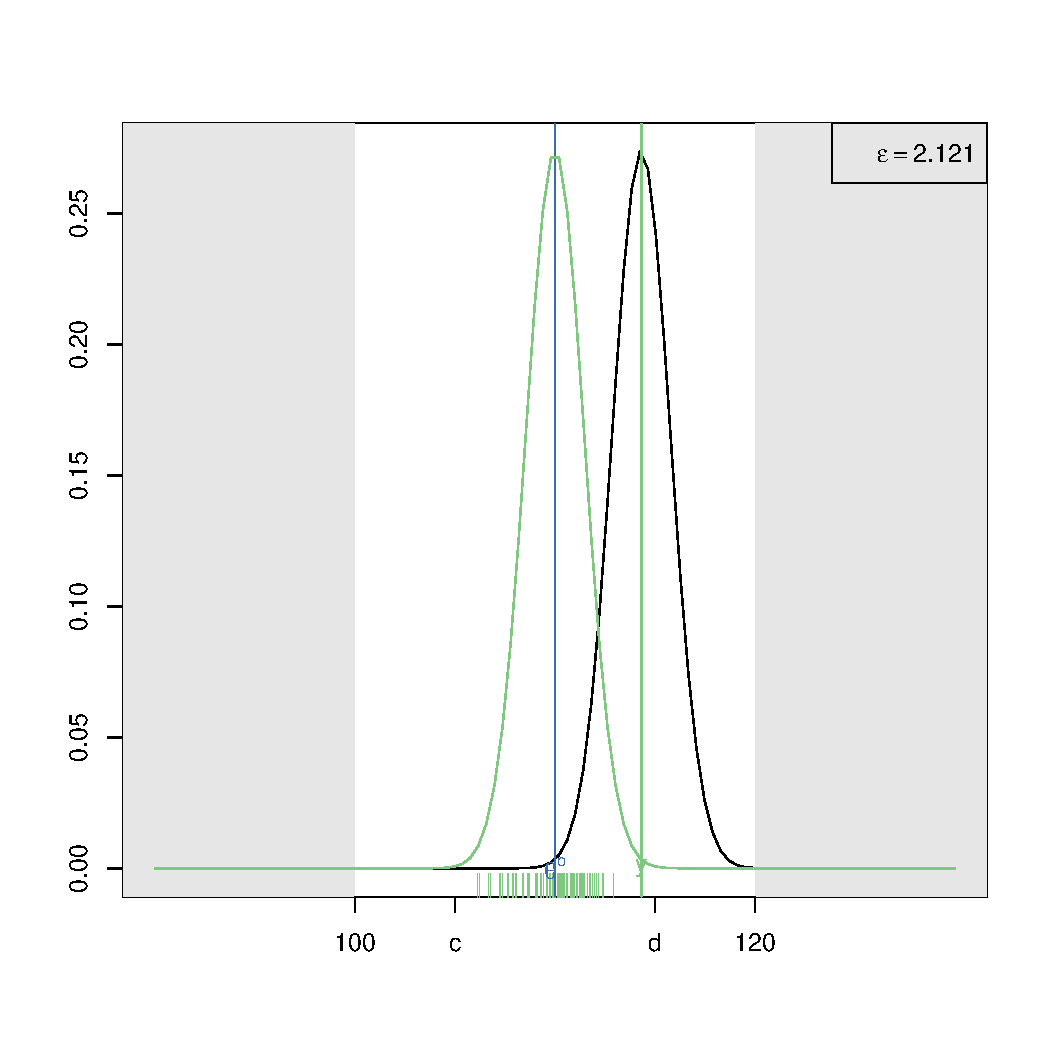
\includegraphics[scale=.35]{./Images/concentrate_30.pdf}}%
\only<32>{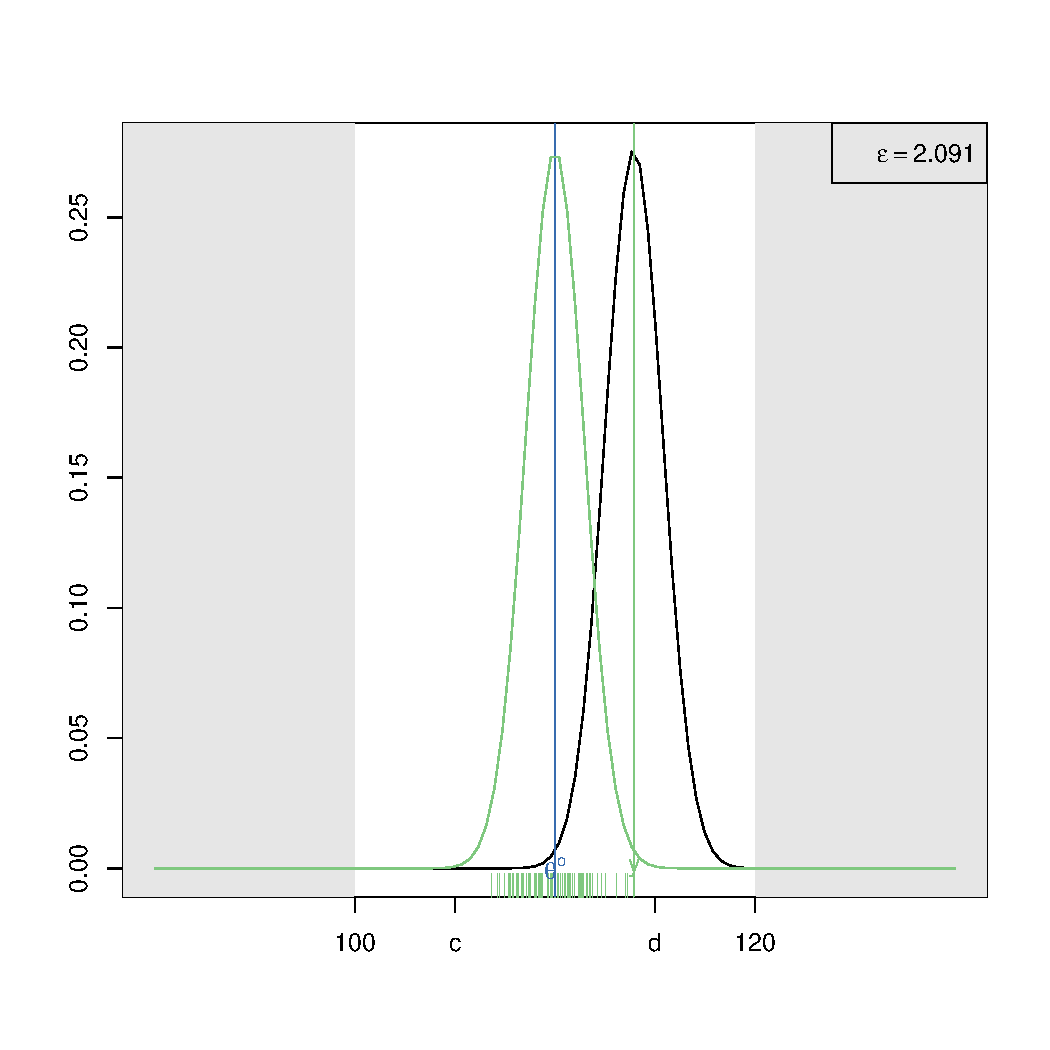
\includegraphics[scale=.35]{./Images/concentrate_31.pdf}}%
\only<33>{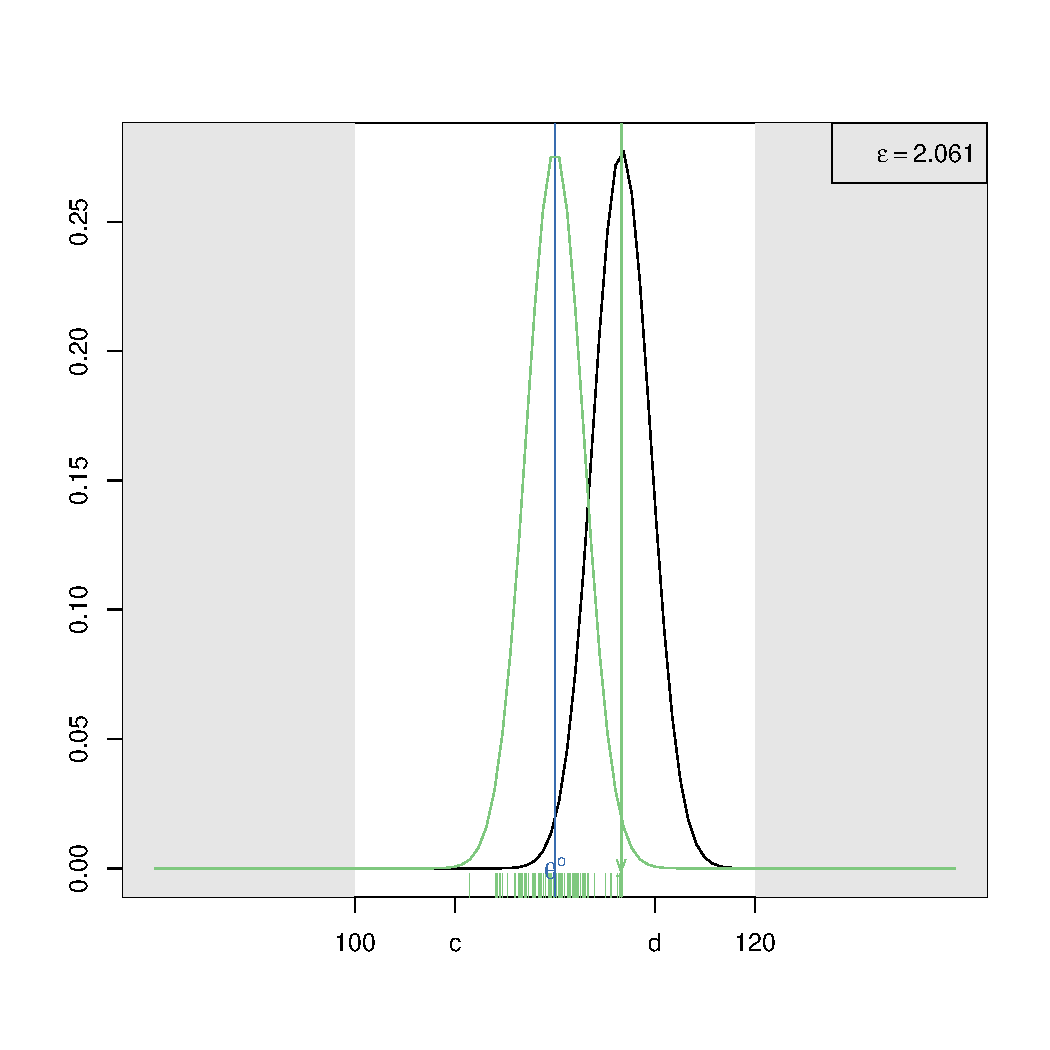
\includegraphics[scale=.35]{./Images/concentrate_32.pdf}}%
\only<34>{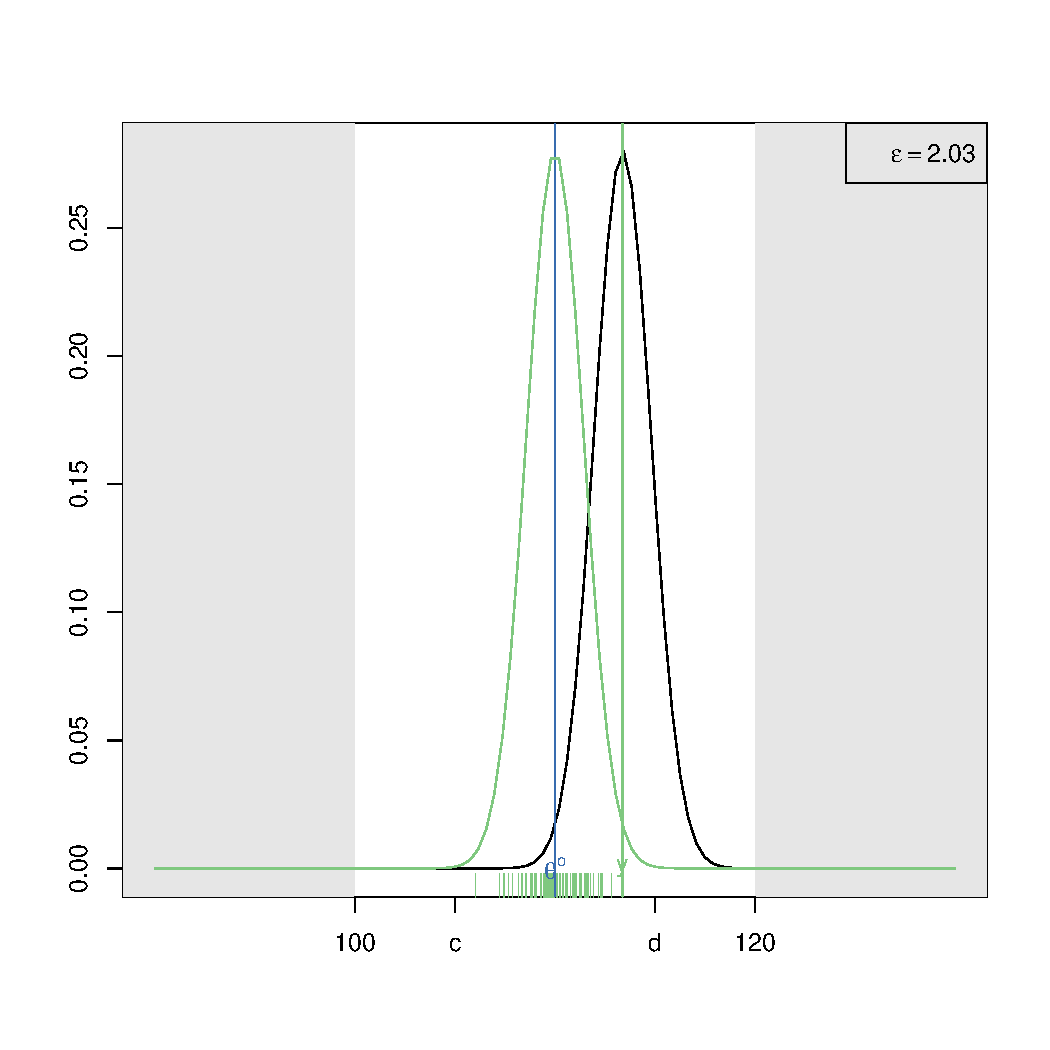
\includegraphics[scale=.35]{./Images/concentrate_33.pdf}}%
\only<35>{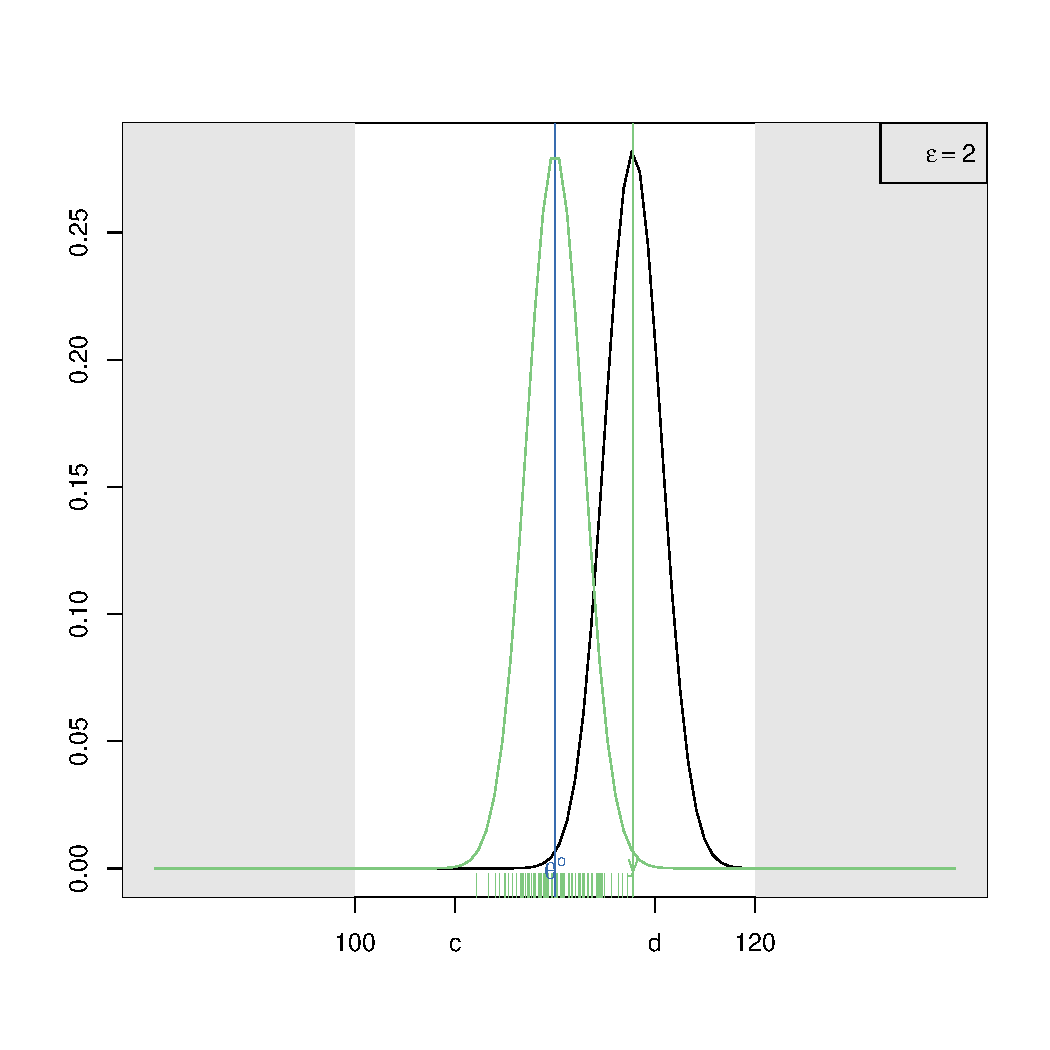
\includegraphics[scale=.35]{./Images/concentrate_34.pdf}}%
\only<36>{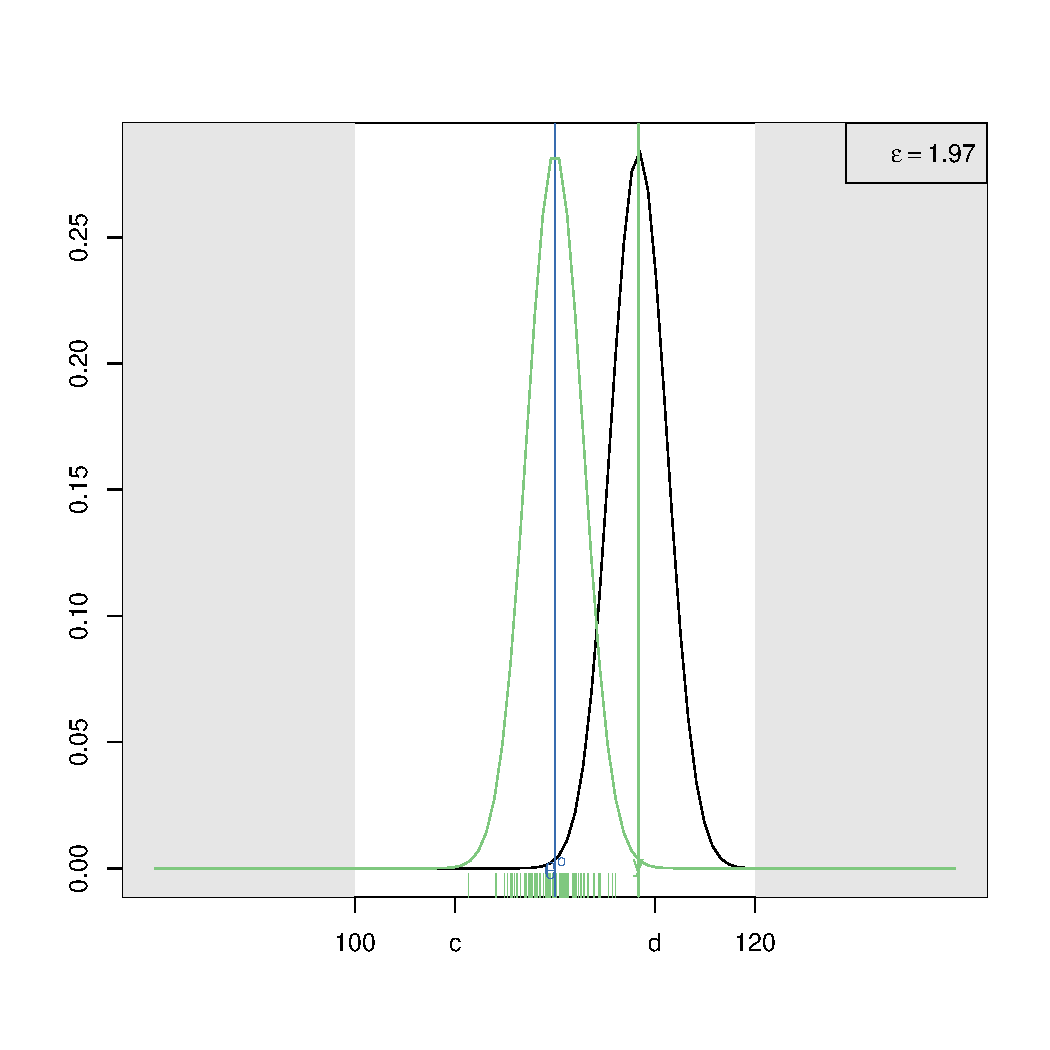
\includegraphics[scale=.35]{./Images/concentrate_35.pdf}}%
\only<37>{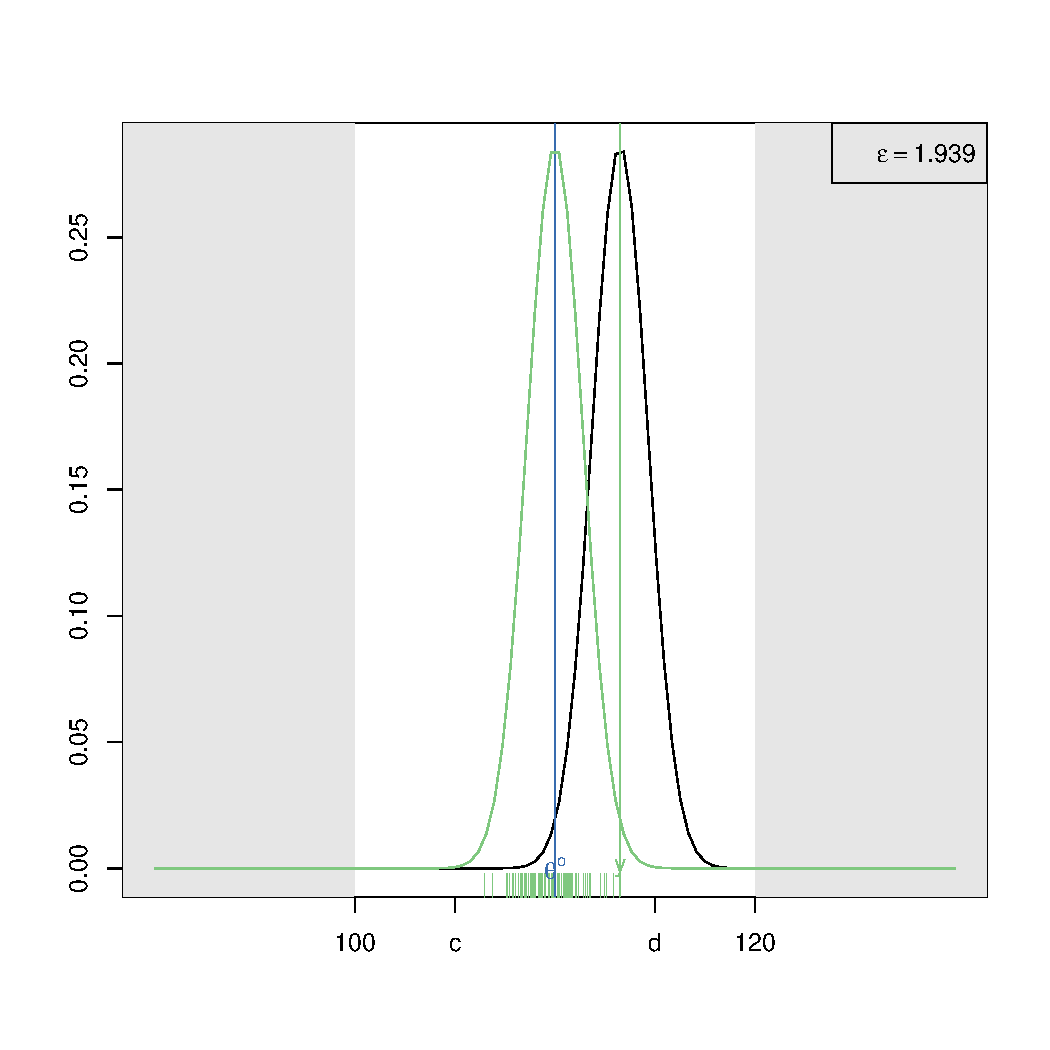
\includegraphics[scale=.35]{./Images/concentrate_36.pdf}}%
\only<38>{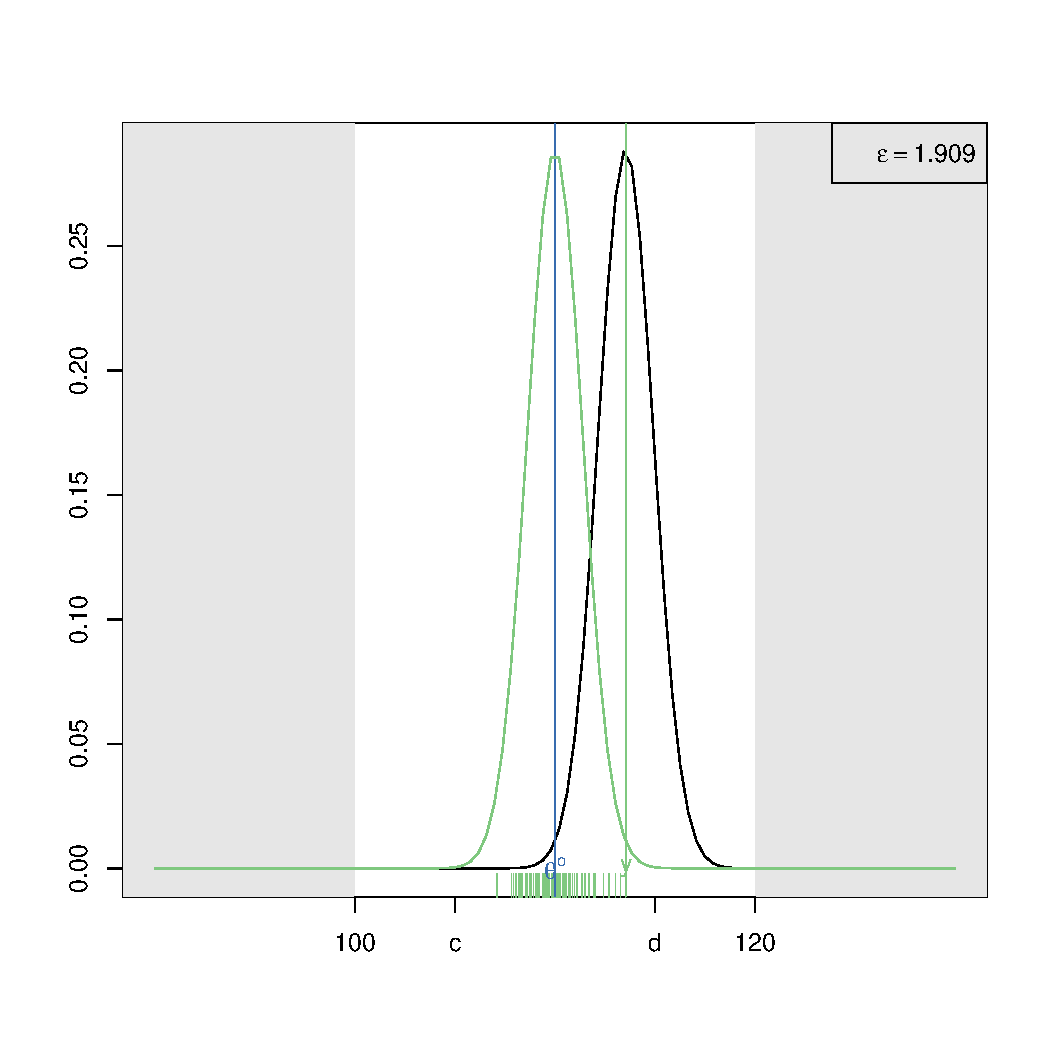
\includegraphics[scale=.35]{./Images/concentrate_37.pdf}}%
\only<39>{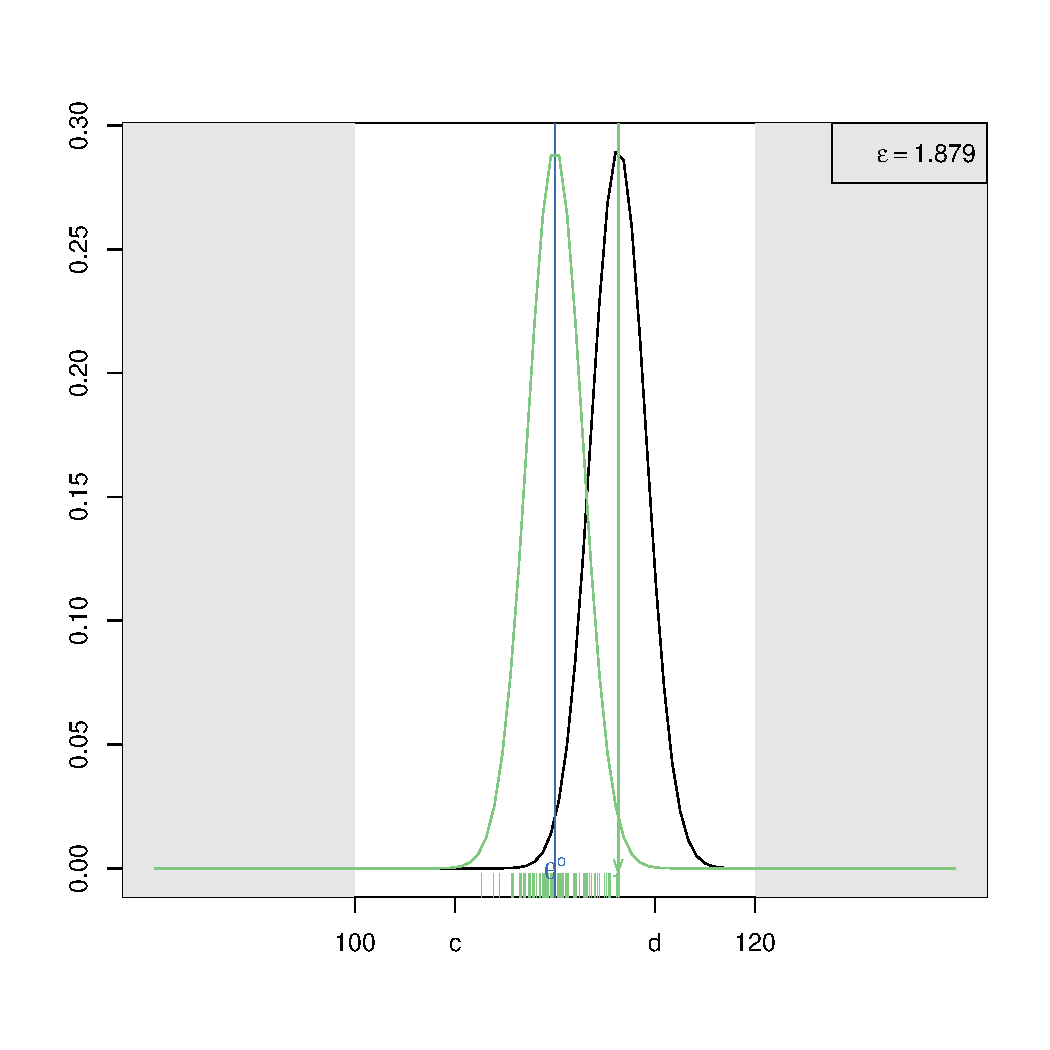
\includegraphics[scale=.35]{./Images/concentrate_38.pdf}}%
\only<40>{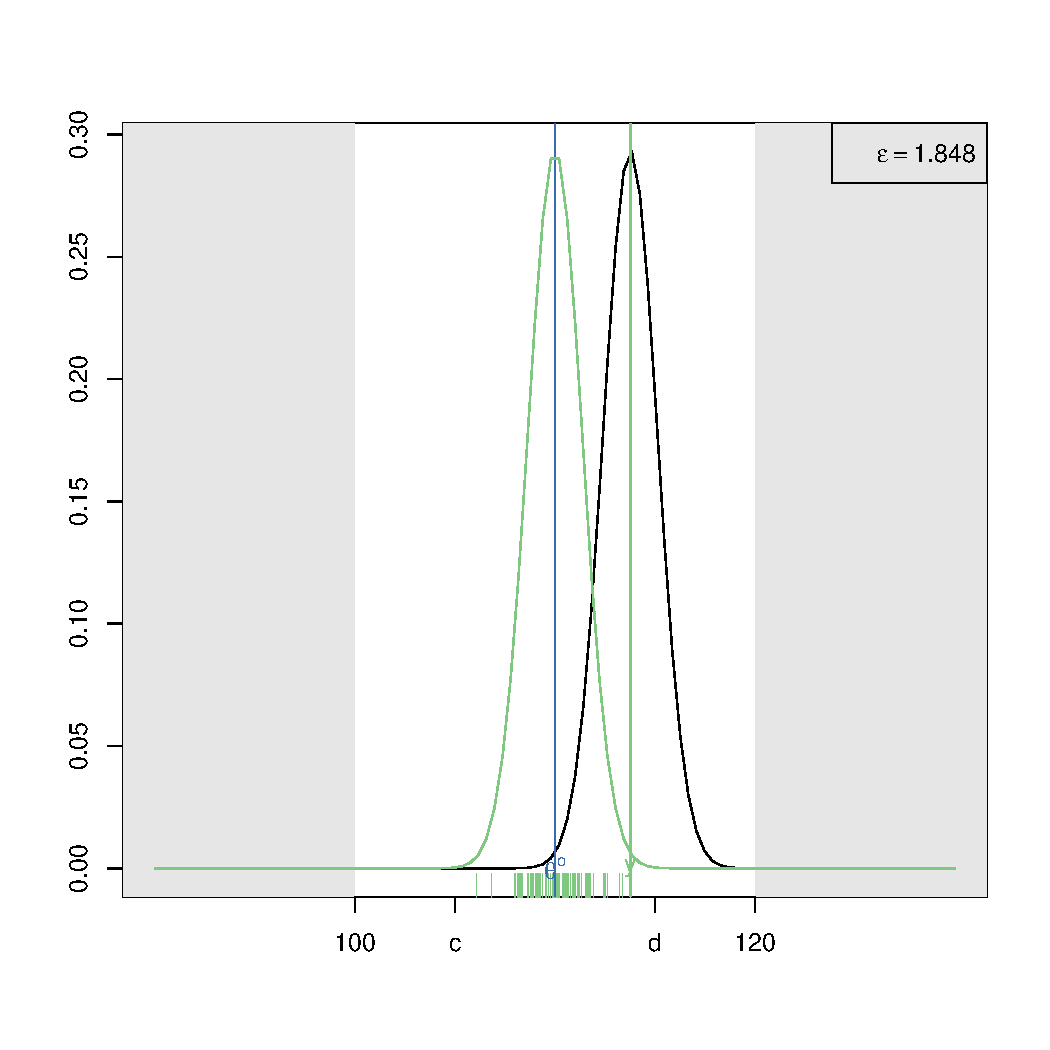
\includegraphics[scale=.35]{./Images/concentrate_39.pdf}}%
\only<41>{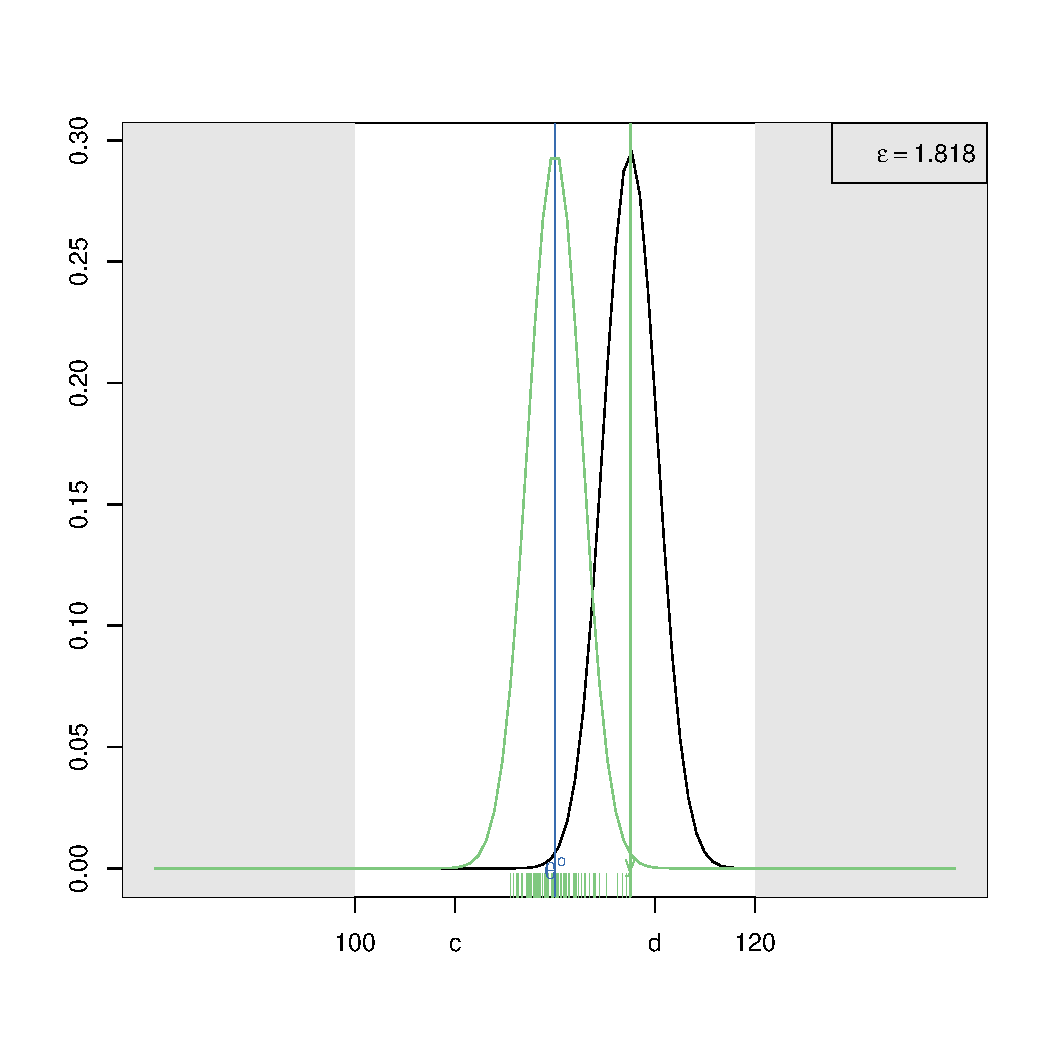
\includegraphics[scale=.35]{./Images/concentrate_40.pdf}}%
\only<42>{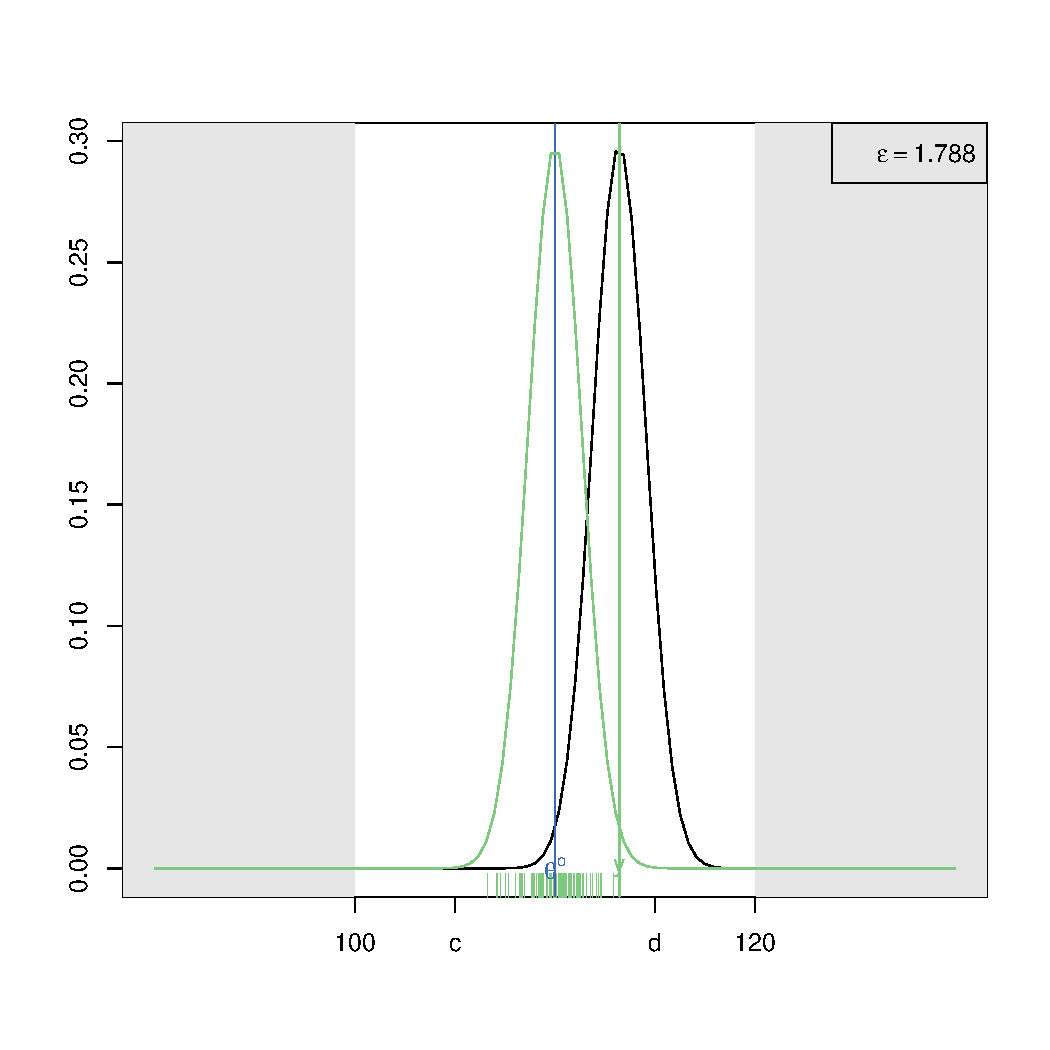
\includegraphics[scale=.35]{./Images/concentrate_41.pdf}}%
\only<43>{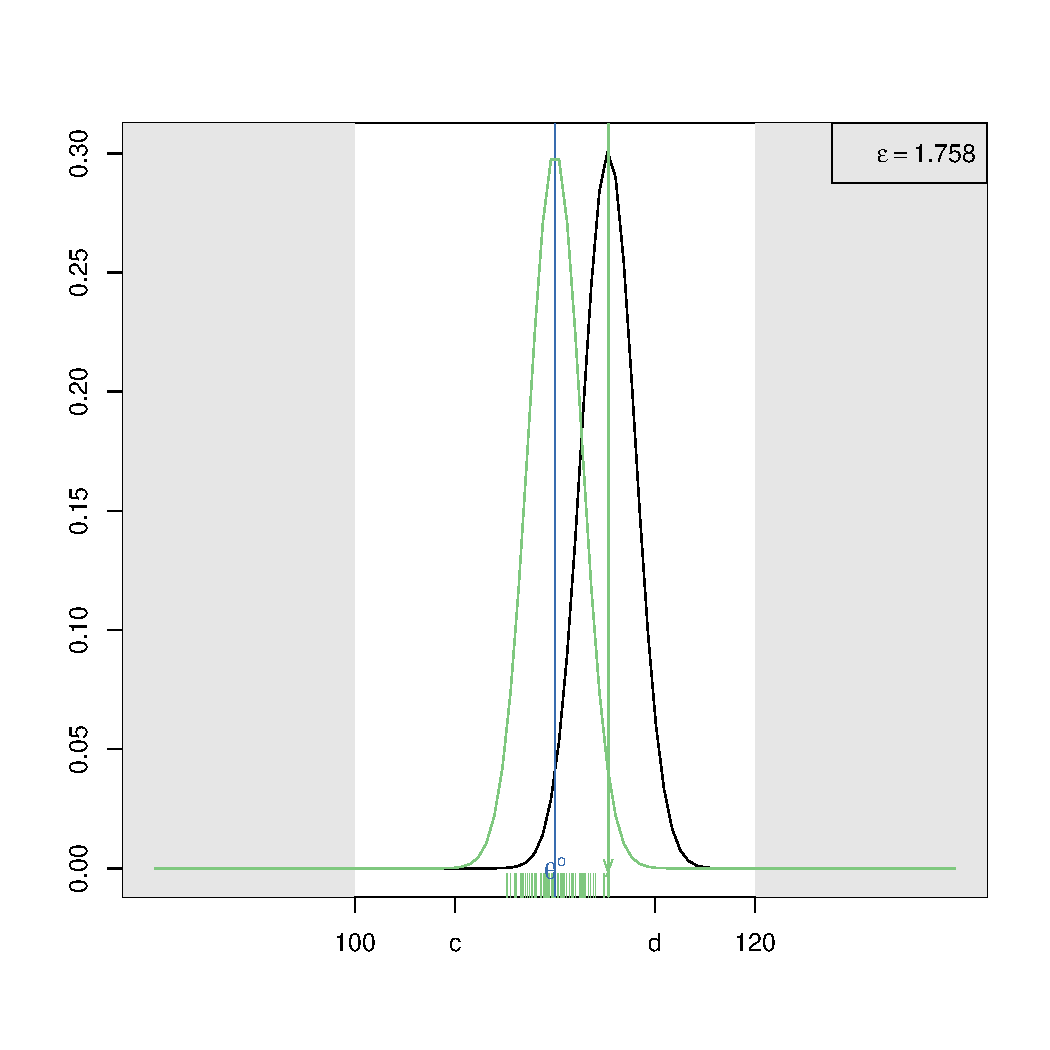
\includegraphics[scale=.35]{./Images/concentrate_42.pdf}}%
\only<44>{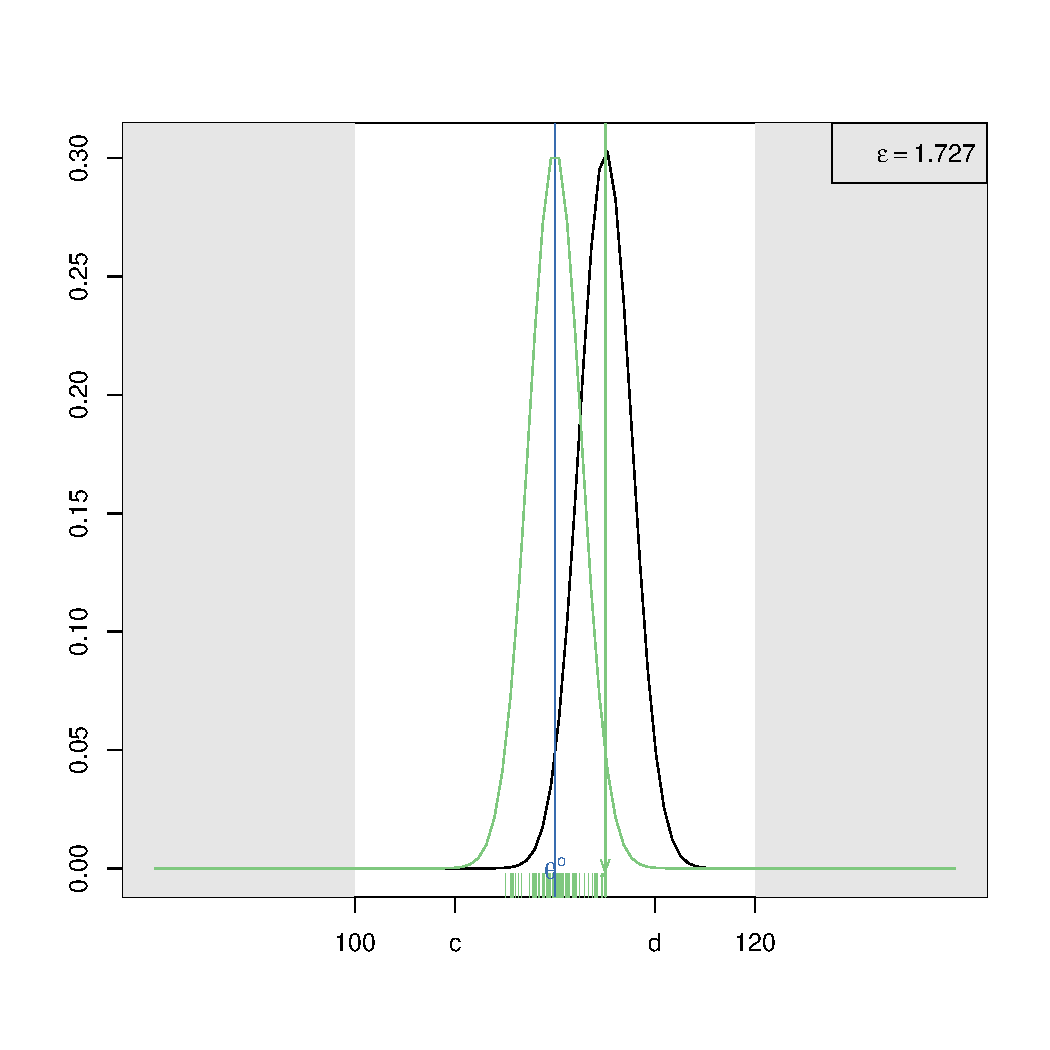
\includegraphics[scale=.35]{./Images/concentrate_43.pdf}}%
\only<45>{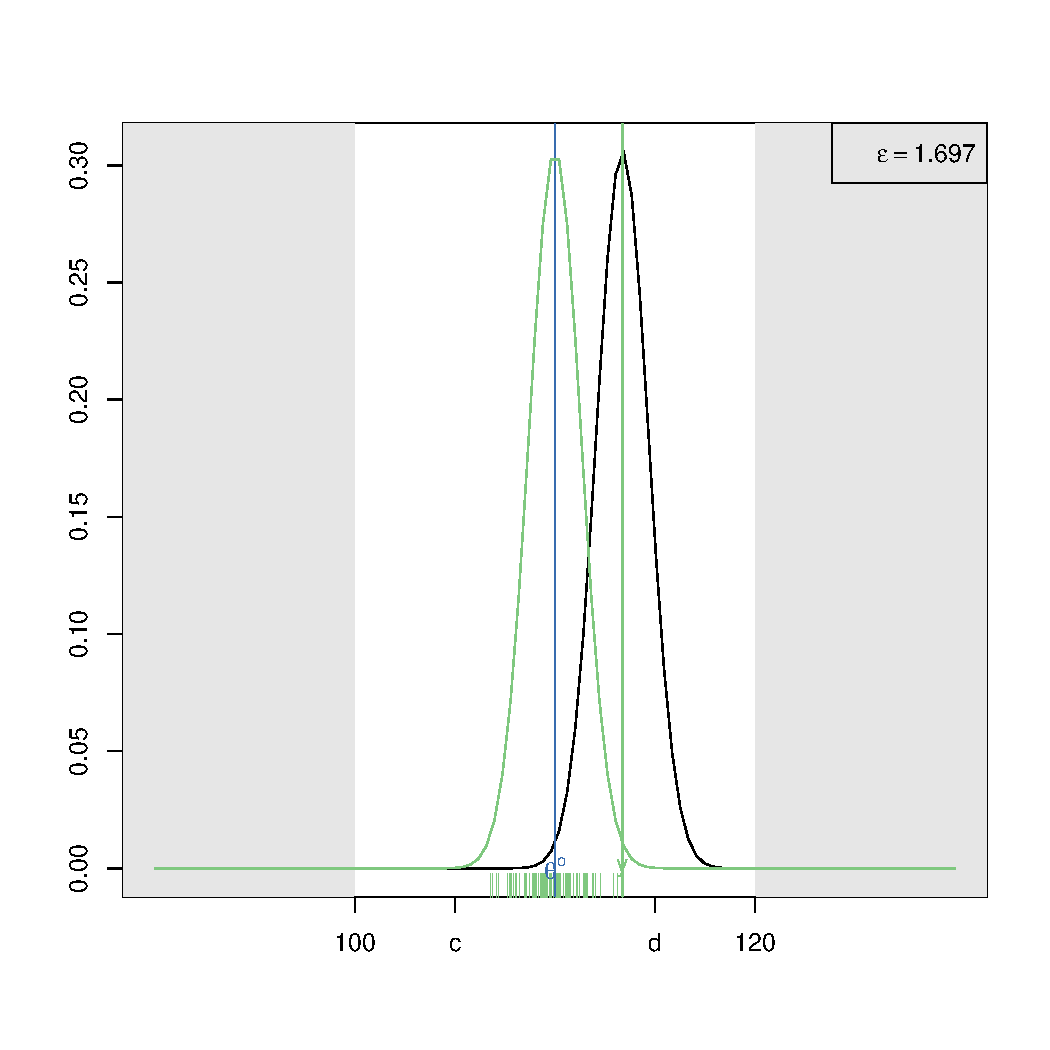
\includegraphics[scale=.35]{./Images/concentrate_44.pdf}}%
\only<46>{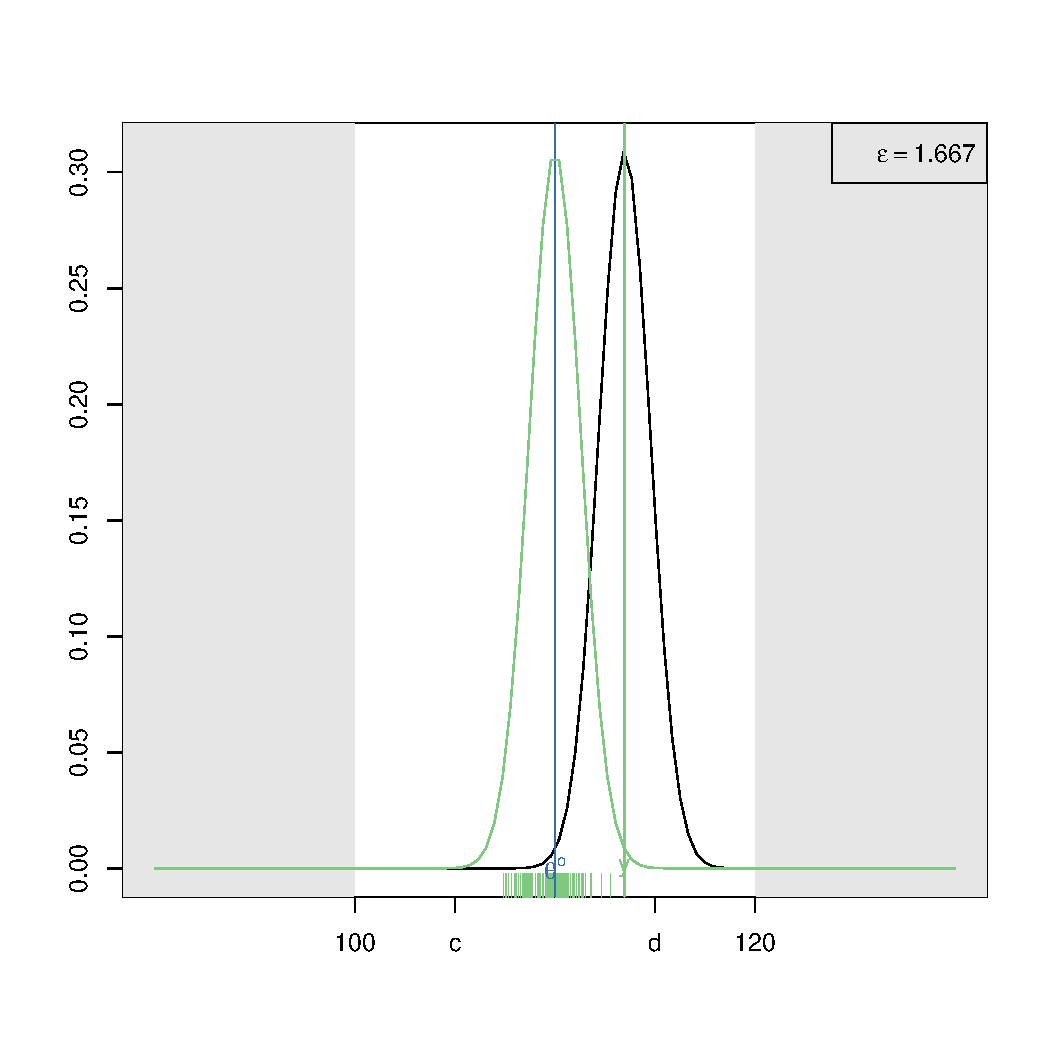
\includegraphics[scale=.35]{./Images/concentrate_45.pdf}}%
\only<47>{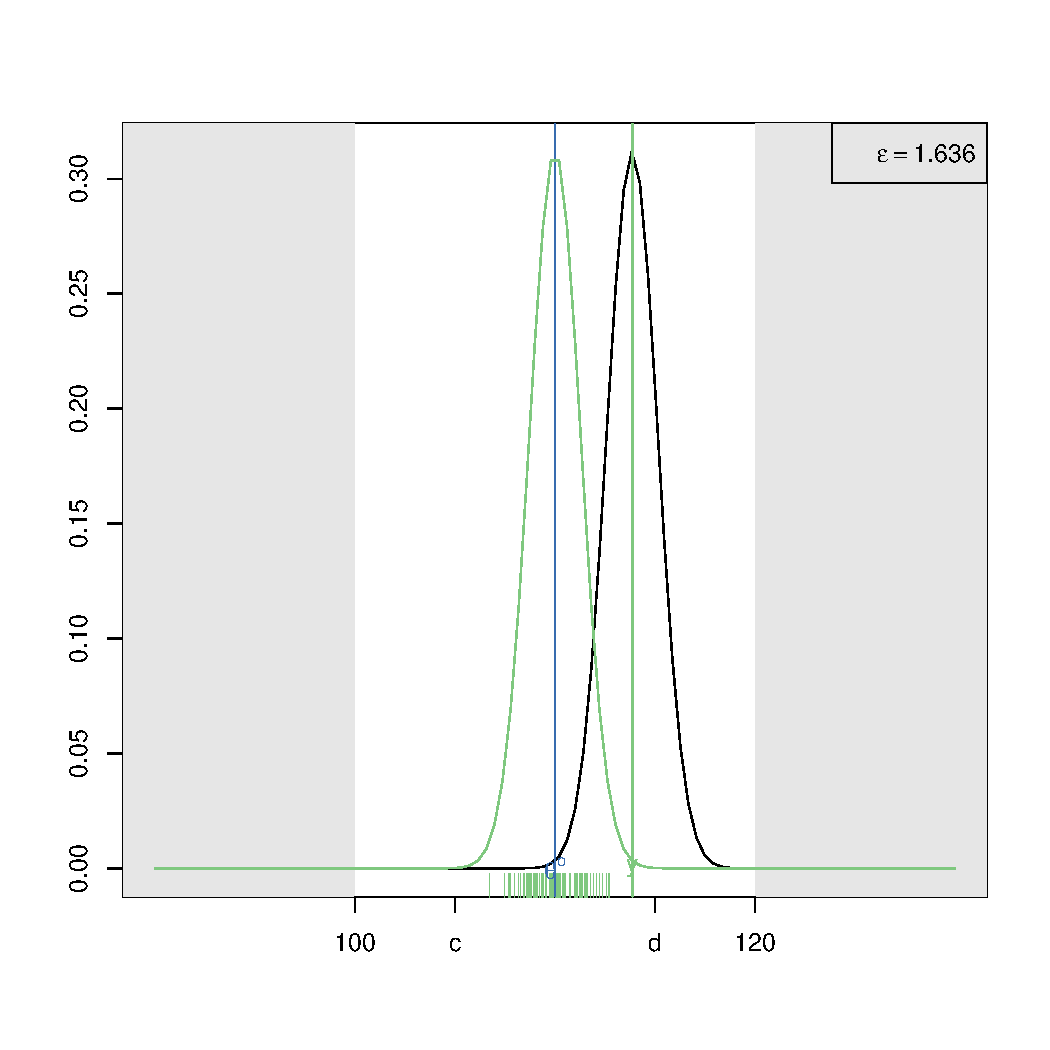
\includegraphics[scale=.35]{./Images/concentrate_46.pdf}}%
\only<48>{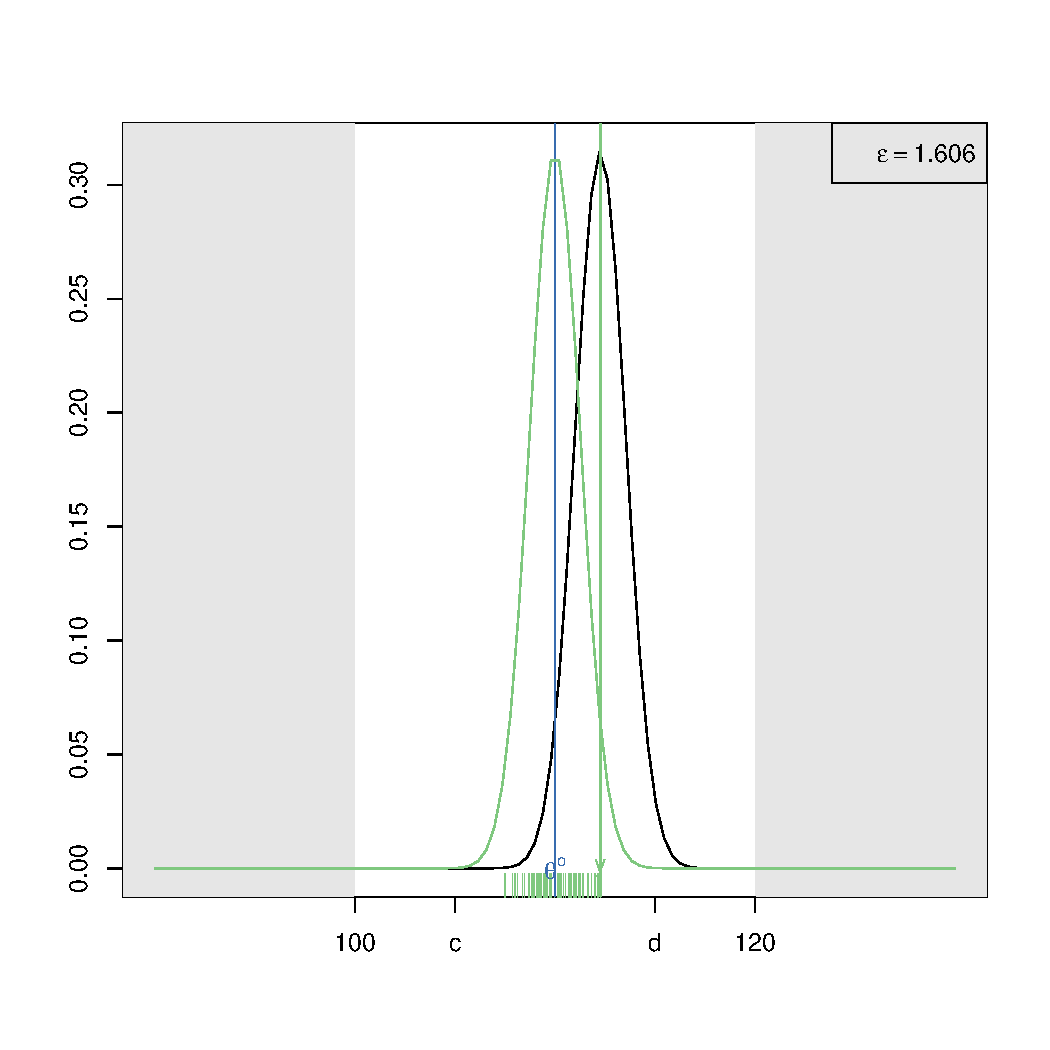
\includegraphics[scale=.35]{./Images/concentrate_47.pdf}}%
\only<49>{\includegraphics[scale=.35]{./Images/concentrate_48.pdf}}%
\only<50>{\includegraphics[scale=.35]{./Images/concentrate_49.pdf}}%
\only<51>{\includegraphics[scale=.35]{./Images/concentrate_50.pdf}}%
\only<52>{\includegraphics[scale=.35]{./Images/concentrate_51.pdf}}%
\only<53>{\includegraphics[scale=.35]{./Images/concentrate_52.pdf}}%
\only<54>{\includegraphics[scale=.35]{./Images/concentrate_53.pdf}}%
\only<55>{\includegraphics[scale=.35]{./Images/concentrate_54.pdf}}%
\only<56>{\includegraphics[scale=.35]{./Images/concentrate_55.pdf}}%
\only<57>{\includegraphics[scale=.35]{./Images/concentrate_56.pdf}}%
\only<58>{\includegraphics[scale=.35]{./Images/concentrate_57.pdf}}%
\only<59>{\includegraphics[scale=.35]{./Images/concentrate_58.pdf}}%
\only<60>{\includegraphics[scale=.35]{./Images/concentrate_59.pdf}}%
\only<61>{\includegraphics[scale=.35]{./Images/concentrate_60.pdf}}%
\only<62>{\includegraphics[scale=.35]{./Images/concentrate_61.pdf}}%
\only<63>{\includegraphics[scale=.35]{./Images/concentrate_62.pdf}}%
\only<64>{\includegraphics[scale=.35]{./Images/concentrate_63.pdf}}%
\only<65>{\includegraphics[scale=.35]{./Images/concentrate_64.pdf}}%
\only<66>{\includegraphics[scale=.35]{./Images/concentrate_65.pdf}}%
\only<67>{\includegraphics[scale=.35]{./Images/concentrate_66.pdf}}%
\only<68>{\includegraphics[scale=.35]{./Images/concentrate_67.pdf}}%
\only<69>{\includegraphics[scale=.35]{./Images/concentrate_68.pdf}}%
\only<70>{\includegraphics[scale=.35]{./Images/concentrate_69.pdf}}%
\only<71>{\includegraphics[scale=.35]{./Images/concentrate_70.pdf}}%
\only<72>{\includegraphics[scale=.35]{./Images/concentrate_71.pdf}}%
\only<73>{\includegraphics[scale=.35]{./Images/concentrate_72.pdf}}%
\only<74>{\includegraphics[scale=.35]{./Images/concentrate_73.pdf}}%
\only<75>{\includegraphics[scale=.35]{./Images/concentrate_74.pdf}}%
\only<76>{\includegraphics[scale=.35]{./Images/concentrate_75.pdf}}%
\only<77>{\includegraphics[scale=.35]{./Images/concentrate_76.pdf}}%
\only<78>{\includegraphics[scale=.35]{./Images/concentrate_77.pdf}}%
\only<79>{\includegraphics[scale=.35]{./Images/concentrate_78.pdf}}%
\only<80>{\includegraphics[scale=.35]{./Images/concentrate_79.pdf}}%
\only<81>{\includegraphics[scale=.35]{./Images/concentrate_80.pdf}}%
\only<82>{\includegraphics[scale=.35]{./Images/concentrate_81.pdf}}%
\only<83>{\includegraphics[scale=.35]{./Images/concentrate_82.pdf}}%
\only<84>{\includegraphics[scale=.35]{./Images/concentrate_83.pdf}}%
\only<85>{\includegraphics[scale=.35]{./Images/concentrate_84.pdf}}%
\only<86>{\includegraphics[scale=.35]{./Images/concentrate_85.pdf}}%
\only<87>{\includegraphics[scale=.35]{./Images/concentrate_86.pdf}}%
\only<88>{\includegraphics[scale=.35]{./Images/concentrate_87.pdf}}%
\only<89>{\includegraphics[scale=.35]{./Images/concentrate_88.pdf}}%
\only<90>{\includegraphics[scale=.35]{./Images/concentrate_89.pdf}}%
\only<91>{\includegraphics[scale=.35]{./Images/concentrate_90.pdf}}%
\only<92>{\includegraphics[scale=.35]{./Images/concentrate_91.pdf}}%
\only<93>{\includegraphics[scale=.35]{./Images/concentrate_92.pdf}}%
\only<94>{\includegraphics[scale=.35]{./Images/concentrate_93.pdf}}%
\only<95>{\includegraphics[scale=.35]{./Images/concentrate_94.pdf}}%
\only<96>{\includegraphics[scale=.35]{./Images/concentrate_95.pdf}}%
\only<97>{\includegraphics[scale=.35]{./Images/concentrate_96.pdf}}%
\only<98>{\includegraphics[scale=.35]{./Images/concentrate_97.pdf}}%
\only<99>{\includegraphics[scale=.35]{./Images/concentrate_98.pdf}}%
\only<100>{\includegraphics[scale=.35]{./Images/concentrate_99.pdf}}}
\end{frame}
% --------------------------------------------------------------------
% <<Intro-F9>>
% --------------------------------------------------------------------
\bframeVL{1-12}{12}
  \frametitle{{\dgrau A glimpse to the essential:} exact posterior  concentration}
\begin{overlayarea}{\textwidth}{.9\textheight}
\begin{columns}\begin{column}[T]{.6\textwidth}%
  Given prior $P_{\RvSo}$ {\dronly{1-}find $\Ra_\ObSoNoL\dwonly{1} \to 0$}\invisible<1>{ as $\ObSoNoL\to 0$ such that
  for $P_{\TrSo}=P_{\ObSo|\RvSo=\TrSo}$}
\begin{dbListeT}[\setListeL{2ex}{2ex}{5ex}{5ex}] 
   \item<2-> $P_{\RvSo|\ObSo} ( \normV{\RvSo-\TrSo}\lesssim {\dr\Ra_\ObSoNoL})\stackrel{P_{\TrSo}}{\to} 1$
   \item<6-> $P_{\RvSo|\ObSo} ( \normV{\RvSo-\TrSo}\gtrsim {\dr\Ra_\ObSoNoL})\stackrel{P_{\TrSo}}{\to} 1$
   \end{dbListeT}
\mywboxinvisible{-9}{{\dgrau Remarks:}
\begin{dshListeT}[\setListeL{2ex}{2ex}{5ex}{5ex}] 
 \item<10-> $\dr\Ra_\ObSoNoL$ depends on the prior
  \item<11-> $\dr\Ra_\ObSoNoL$ might be arbitrarily slow
  \item<12-> consistency could fail
  \end{dshListeT}}
\end{column}\begin{column}[T]{.4\textwidth}%
\hspace*{4ex}\includegraphics<1>[scale=.8]{./Images/reg.31}%
\includegraphics<2>[scale=.8]{./Images/reg.31}%
\includegraphics<3>[scale=.8]{./Images/reg.32}%
\includegraphics<4>[scale=.8]{./Images/reg.33}%
\includegraphics<5>[scale=.8]{./Images/reg.34}%
\includegraphics<6>[scale=.8]{./Images/reg.35}%
\includegraphics<7>[scale=.8]{./Images/reg.36}%
\includegraphics<8>[scale=.8]{./Images/reg.37}%
\includegraphics<9->[scale=.8]{./Images/reg.38}%
%\begin{textblock}{6}(2,14.5) \only<1->{{\db Parameter of interest}}\end{textblock} 
%\begin{textblock}{6}(9.5,14.5)\only<1->{{\db Transformed  parameter}}\end{textblock} 
\end{column}
\end{columns}
\end{overlayarea}
\end{frame}


% --------------------------------------------------------------------
% <<References>>
% --------------------------------------------------------------------
\begin{frame}
\frametitle{}
{\small{\begin{thebibliography}{10}       
\beamertemplatearticlebibitems

\bibitem{[1]}\dg {S. Ghosal, J.K. Ghosh and  A.W. Van Der Vaart} (2000)
{\ds\it Convergence rates of posterior distributions.}
{\ds The Annals of Statistics 28(2):500–531}

\bibitem{[2]}\dg {X. Shen and L. Wasserman.} (2001) 
{\ds\it Rates of convergence of posterior distributions.}
{\ds The Annals of Statistics, 29:687–714}


\bibitem{[3]}\dg {B. Knapik, A. Van der Vaart, and J. Van Zanten} (2011) 
{\ds\it Bayesian inverse problems with gaussian priors.}
{\ds The Annals of Statistics, 39:2626–2657}

\bibitem{[4]}\dg {J. Arbel, G. Gayraud and J. Rousseau} (2013) 
{\ds\it Bayesian optimal adaptive estimation using a sieve prior.}
 {\ds Scandinavian Jounral of Statistics, 40:549--570}

% \bibitem{[5]}\dg {B. Knapik, B. Szabó, A. Van der Vaart, and J. Van
%     Zanten} (2014)
% {\ds\it Bayes procedures for adaptive inference in inverse problems
%   for the white noise model.}
% {\ds Preprint, arXiv:1209.3628v2}

\bibitem{[6]}\dg {K. Ray} (2013)
{\ds\it Bayesian inverse problems with non-conjugate priors.} 
{\ds Electronic Journal of Statistics, 7: 2516–2549}

\bibitem{[7]}\dg {M. Hoffmann, J. Rousseau  and  J. Schmidt-Hieber} (2015) {\ds\it On adpative posterior concentration rates.} 
{\ds The Annals of Statistics, 43:5,2259--2295}

 \bibitem{[8]}\dg  {I. Castillo} (2008) 
{\ds \it Lower bounds for posterior rates with Gaussian process  priors.}
{\ds Electronic Journal of Statistics, 2:1281-1299}
\end{thebibliography}}}
\end{frame}


% --------------------------------------------------------------------
% <<Intro-F10>>
% --------------------------------------------------------------------
\bframeVL{1-3}{3}[label=Op]
\frametitle{{\rudicolor  Objective:} exact posterior concentration}
\begin{rudiListeS}[\setListeL{4ex}{2ex}{5ex}{5ex}] 
\item Construct   a family  $\{P_{\DiRvSo}\}_{\Di}$ of prior
  distributions with\\[1ex]
{\dr exact} posterior  concentration $\eRa^{\eDi}:=\eRa^{\eDi}(\TrSo)$ for $\TrSo\in\cSo$,
  i.e.,
\[\lim_{\ObSoNoL\to0} \Ex_{\TrSo}
P_{\hspace*{-.8ex}\DiRvSo[\eDi]|\ObSo}\Bigl(\eRa^{\eDi} \lesssim
\normV{\DiRvSo[\eDi]-\TrSo}^2\lesssim \eRa^{\eDi}\Bigr)=1;\]
\begin{rudiListeT}[\setListeL{2ex}{5ex}{2ex}{0ex}] 
\item<2-> Consider for a given $\TrSo\in\cSo$ the {\rudicolor oracle} rate
\[\treRa:=\treRa(\TrSo):=\inf_{\Di}\,\eRa^{\Di}(\TrSo).  \]
% \item<5-> Consider for a given $\cwSo\subset\cSo$  the {\rudicolor minimax} rate
% \[\oeRa:=\oeRa(\wSo):=\inf_{\tSo}\sup_{\TrSo\in\cwSo}\Ex_{\TrSo}\normV{\tSo-\TrSo}^2.  \]
\item<3-> Consider for a given $\cwSo\subset\cSo$  the {\rudicolor minimax} rate
\[\oeRa:=\oeRa(\wSo):=\inf_{\Di}\sup_{\TrSo\in\cwSo}\eRa^{\Di}(\TrSo).  \]
\end{rudiListeT}
\end{rudiListeS}
\end{frame}

% --------------------------------------------------------------------
% <<Intro-F11>>
% --------------------------------------------------------------------
\bframeVL{1-2}{2}[label=OPC]
\frametitle{{\rudicolor Objective:} optimal prior choice}
\begin{rudiListeS}[\setListeL{4ex}{2ex}{5ex}{5ex}] 
\item A  sub-family $\{P_{\hspace*{-.8ex}\DiRvSo[\treDi]}\}_{\treDi}$
  with {\rudicolor exact} posterior  concentration   $\treRa$, i.e.
\[\lim_{\ObSoNoL\to0} \Ex_{\TrSo} P_{\hspace*{-.8ex}\DiRvSo[\treDi]|\ObSo}\Bigl(\treRa \lesssim \normV{\DiRvSo[\treDi]-\TrSo}^2\lesssim \treRa  \Bigr)=1, \]  
is called {\rudicolor oracle} prior  and {\dr adaptive} if it
does not depend on $\TrSo$.
% \item<3-> and  a Bayes estimate
%   $\hDiSo[\treDi]:=\Ex[\DiRvSo[\treDi]|\ObSo]$ satisfying
%   \[  \Ex_{\TrSo}\normV{\hDiSo[\treDi]-\TrSo}^2\lesssim \treRa \]   
% is called ``oracle Bayes estimate''.
% \item Consider for given $\cwSo\subset\cSo$  the minimax rate
% \[\oeRa:=\oeRa(\wSo):=\inf_{\tSo}\sup_{\TrSo\in\cwSo}\Ex_{\TrSo}\normV{\tSo-\TrSo}^2.  \]
\item<2-> A sub-family $\{P_{\hspace*{-.8ex}\DiRvSo[\oeDi]}\}_{\oeDi}$
  with {\rudicolor exact} posterior
  concentration  $\oeRa$, i.e.
\[\lim_{\ObSoNoL\to0}  \inf_{\TrSo\in\cwSo} \Ex_{\TrSo}P_{\hspace*{-.8ex}\DiRvSo[\oeDi]|\ObSo}\Bigl(\oeRa\lesssim
  \normV{\DiRvSo[\oeDi]-\TrSo}^2\lesssim \oeRa  \Bigr)=1.
  \]  
is called {\rudicolor minimax} prior and {\dr adaptive} if it
depends not on $\cwSo$.
% \item<3-> and  a Bayes estimate
%   $\hDiSo[\oeDi]:=\Ex[\DiRvSo[\oeDi]|\ObSo]$ satisfying
%   \[ \sup_{\TrSo\in\cwSo} \Ex_{\TrSo}\normV{\hDiSo[\oeDi]-\TrSo}^2\lesssim \oeRa \]   
% is called ``minimax Bayes estimate''.
\end{rudiListeS}
\end{frame}



% % --------------------------------------------------------------------
% % <<Intro-F1>>
% % --------------------------------------------------------------------
% \bframeVL{22-34}{34}[label=IIP]
% \frametitle{\only<22-31>{{\dgrau A glimpse to the
%     essential:} {{\dwonly{22-27}statistical} {\dwonly{22-24}inverse
%     problem}}}\only<32-35>{{\dgrau Considered framework:} ill-posed
% inverse problem}}
% \centerline{%
% \includegraphics<22>[scale=.8]{./Images/inv.1}%
% \includegraphics<23>[scale=.8]{./Images/inv.2}%
% \includegraphics<24>[scale=.8]{./Images/inv.3}%
% \includegraphics<25>[scale=.8]{./Images/inv.4}%
% %\includegraphics<30>[scale=.9]{./Images/inv.5}
% \includegraphics<26>[scale=.8]{./Images/inv.6}%
% \includegraphics<27>[scale=.8]{./Images/inv.7}%
% \includegraphics<28>[scale=.8]{./Images/inv.8}%
% \includegraphics<29>[scale=.8]{./Images/inv.9}%
% \includegraphics<30>[scale=.8]{./Images/inv.10}%
% \includegraphics<31>[scale=.8]{./Images/inv.11}%
% \includegraphics<32>[scale=.8]{./Images/inv.12}%
% \includegraphics<33>[scale=.8]{./Images/inv.13}%
% \includegraphics<34,35>[scale=.8]{./Images/inv.14}%
% \includegraphics<35>[scale=.8]{./Images/inv.15}%
% }
% \begin{textblock}{6}(2,14.5) \only<22->{{\dgrau Function of interest}}\end{textblock} 
% \begin{textblock}{6}(9.5,14.5)\only<24->{{\dgrau Transformed  function}}\end{textblock} 
% \begin{textblock}{6}(7,4.5)\only<26>{{\db Existence
%       ?}}\only<27>{{\db Identified ?}}\only<29-31>{{\db Stability ?}}\end{textblock} 
% \begin{textblock}{6}(6.3,10.5)\only<32->{{\dr
%       Stability: no!}} \end{textblock} 
% \begin{textblock}{6}(6.3,6.9)\only<33->{{\dg Identified: assumed.}} \end{textblock} 
% \begin{textblock}{6}(6.3,4.5)\only<34>{{\dg Existence:
%       assumed.}} \end{textblock} 

% \begin{textblock}{6}(11.5,11)\small\only<28>{{\dgrau Estimator}}\end{textblock} 
% \begin{textblock}{6}(3,11)\small\only<28>{{\dgrau Estimator}}\end{textblock} 
% % \begin{textblock}{6}(2,14.5) \only<22->{{\dgrau Parameter of interest}}\end{textblock} 
% % \begin{textblock}{6}(9.5,14.5)\only<24->{{\dgrau Transformed  parameter}}\end{textblock} 
% % \begin{textblock}{6}(7,4.5)\only<26,34>{{\dgrau Existence ?}}\only<27,33>{{\dg Identified ?}}\only<29-32>{{\dg Stability ?}} \end{textblock} 
% % \begin{textblock}{6}(10.8,11)\small\only<28>{{\dg\lq\lq Measurement\rq\rq}}\end{textblock} 
% % \begin{textblock}{6}(3,11)\small\only<28>{{\dg Estimator}}\end{textblock} 
% \end{frame}
% % --------------------------------------------------------------------
% % <<Intro-F2>>
% % --------------------------------------------------------------------
% \bframeVL{1-5}{5}
% \frametitle{{\dgrau Background:} analytical inverse problem}
% Consider $(\colF,\skalar)$, $(\colG,\skalar)$ and
% $\colT:\colF\to\colG$ linear\\[1.5ex]
% \hspace*{5ex}{\xymatrix{
% \colf \ar@{|->}[r]^\colT\only<3->{\ar@{<->}[d]}& \colg \only<5->{\ar@{<->}[d]}\\
% \uncover<3->{(\alt<3>{\skalarV{\colf,\colbasF_j}}{\coltheta_j})_{j}}\only<5->{\ar@{|->}[r]^\collambda}& 
% \uncover<5->{(\collambda_j\coltheta_j)_{j}}}}\hfill\\[1.5ex]
% \mywboxinvisible{-1}{{special case}
%  $\colT$ permits a singular value decomposition  
% \begin{rudiListeS}[\setListeL{2ex}{2ex}{5ex}{5ex}] 
%   \item<2-> Singular values $\collambda:=(\collambda_j)_{j}$
%   \item<2-> Eigenfunctions $\{\colbasF_j\}_{j}$ and
%     $\{\colbasG_j\}_{j}$ ONB of $\colF$ and $\colG$, resp.
%   \end{rudiListeS}}

% \mywboxinvisible{-2}{{\rudicolor Representation}
% \begin{rudiListeS}[\setListeL{2ex}{2ex}{5ex}{5ex}] 
%   \item<3-> $ \colf\in \colF$\uncover<4->{$\leftrightarrow \coltheta \in \colTheta:=\ell^2  $ via $\coltheta_j =\skalarV{\colf,\colbasF_j}$} 
%   \item<5-> Operator $\colT \leftrightarrow$ Multiplication with $\collambda$
%   \end{rudiListeS}}
% \end{frame}

% % --------------------------------------------------------------------
% % <<Intro-F16>>
% % --------------------------------------------------------------------
% \bframeVL{1-4}{4}
% \frametitle{{\dgrau A glimpse to the essential:} posterior
%   concentration rate}
% \centerline{%
% \includegraphics<1>[scale=.8]{./Images/reg.15}%
% \includegraphics<2>[scale=.8]{./Images/reg.16}%
% \includegraphics<3>[scale=.8]{./Images/reg.17}%
% \includegraphics<4>[scale=.8]{./Images/reg.18}%
% }
% \begin{textblock}{6}(2,14.5) \only<1->{{\db Parameter of interest}}\end{textblock} 
% %\begin{textblock}{6}(9.5,14.5)\only<1->{{\db Transformed  parameter}}\end{textblock} 
% \end{frame}



% % --------------------------------------------------------------------
% % <<Intro-F6>>
% % --------------------------------------------------------------------
% \bframeVL{1-3}{3}
% \frametitle{{\dgrau Frequentist point of view:} upper bound}
% \centerline{%
% \includegraphics<1>[scale=.8]{./Images/gssm.10}%
% \includegraphics<2>[scale=.8]{./Images/gssm.11}%
% \includegraphics<3>[scale=.8]{./Images/gssm.12}%
% }
% \begin{textblock}{6}(2,14.5) \only<1->{{\dgrau Parameter of interest}}\end{textblock} 
% \begin{textblock}{6}(9.5,14.5)\only<1->{{\dgrau Transformed  parameter}}\end{textblock} 
% \end{frame}
% % --------------------------------------------------------------------
% % <<Intro-F5>>
% % --------------------------------------------------------------------
% \bframeVL{1-3}{3}
% \frametitle{{\dgrau Frequentist point of view:} lower bound}
% \centerline{%
% \includegraphics<1>[scale=.8]{./Images/gssm.13}%
% \includegraphics<2>[scale=.8]{./Images/gssm.14}%
% \includegraphics<3>[scale=.8]{./Images/gssm.15}%
% }
% \begin{textblock}{6}(2,14.5) \only<1->{{\dgrau Parameter of interest}}\end{textblock} 
% \begin{textblock}{6}(9.5,14.5)\only<1->{{\dgrau Transformed  parameter}}\end{textblock} 
% \end{frame}
% % --------------------------------------------------------------------
% % <<Intro-F7>>
% % --------------------------------------------------------------------
% \bframeVL{1-4}{1}
% \frametitle{{\dgrau Frequentist point of view:} adaptation}
% \centerline{%
% \includegraphics<1>[scale=.8]{./Images/gssm.20}%
% %\includegraphics<2>[scale=.8]{./Images/reg.20}%
% \includegraphics<2>[scale=.8]{./Images/gssm.22}%
% \includegraphics<3>[scale=.8]{./Images/gssm.23}%
% \includegraphics<4>[scale=.8]{./Images/gssm.24}%
% }
% \begin{textblock}{6}(2,14.5) \only<1->{{\dgrau Parameter of interest}}\end{textblock} 
% \begin{textblock}{6}(9.5,14.5)\only<1->{{\dgrau Transformed  parameter}}\end{textblock} 
% \begin{textblock}{6}(10.8,11)\small\only<1>{{\dgrau Estimator}}\end{textblock} 
% \begin{textblock}{6}(6.4,11)\small\only<1>{{\db Data-driven}}\end{textblock} 
% \begin{textblock}{6}(1.8,11)\small\only<1>{{\db Data-driven}}\end{textblock} 
% \end{frame}




% % --------------------------------------------------------------------
% % <<Intro-F9>>
% % --------------------------------------------------------------------
% %%%%%%%%%%%%%%%%%%%%%
% \bframeVL{1-6}{10}
% \frametitle{{\dgrau A glimpse to the essential:} dimension reduction}
% %\mywbox{\centerline{{\db Reconstruct $\So$} given $\db\oIm =\Op\So + \sqrt\lnIm \nIm$ and $\db\oOp = \Op+ \sqrt\lnOp \nOp$.}}
% Introduce a  sieves sequence  $\dbonly{1}\Uz_1\subset\Uz_2\subset\cdots\subset\Uz_m\subset\cdots\subset\Hspace$.
% \begin{dbListeT}[\setListeL{5ex}{5ex}{2ex}{2ex}] 
% \item<2->  Consider a theoretical approximation  $\dbonly{2}\fSo_m\in \mHspace$  of $\fSo\in\Hspace$ and let %associated approximation error
%   \[\dbonly{2}\gb_m:=\sup\nolimits_{k\geq m}\normV{\fSo_k-\fSo}^2.\]
% \item<3-> Construct an {\dbonly{3}estimator $\hfSo_m$} of $\fSo_m$ based on  $\dbonly{3}\widehat{g}$\dwonly{3}, where 
%   \[\dbonly{4}\Ex_{\fSo}\normV{{\dbonly{4}\hfSo_m}-\fSo}^2\lesssim \dbonly{4}\gb_m(\fSo) + \Ex_{\fSo}\normV{\fSo_m-\hfSo_m}^2.\]
% \item<5-> Derive $\dbonly{5}\gv_m\geq
%   \Ex_{\fSo}\normV{\fSo_m-\hfSo_m}^2$\dwonly{5}, then \[\dbonly{6}
% \Ex_{\fSo}\normV{{\dbonly{6}\hfSo_m}-\fSo}^2\dbonly{6}\lesssim [\gb_m\vee\gv_m]=\max(\gb_m,\gv_m)\text{ for }\dbonly{6}m\geq1.\]
% % \item<7-> Optimal choice $\dbonly{7}\mopte{}:=\argmin\nolimits_m\set{\max( b_m^2,v_m)}$  \dwonly{7}gives  
% % \[\dbonly{8}\Rifes[]{{\dbonly{8}\hSoGa[\mopte{\lnIm,\lnOp}]}}{\cSo,\cOp}\lesssim \dbonly{8}\min\nolimits_m\set{\max( b_m^2,v_m)}=:\oRifes[]{\cSo,\cOp}\]
% % \dwonly{-8}which  establishes {\dbonly{9}minimax-optimality of $\hSoGa[\mopte{}]$}, if \[\dbonly{9}\inf\nolimits_{\tSo}\Rifes[]{{\dbonly{9}\tSo}}{\cSo,\cOp}\gtrsim \dbonly{9}\oRifes[]{\cSo,\cOp}.\]
% \end{dbListeT}
% \end{frame}
% % --------------------------------------------------------------------
% % <<Intro-F10>>
% % --------------------------------------------------------------------
% %%%%%%%%%%%%%%%%%%%%%
% \bframeVL{6-9}{10}
% \frametitle{{\dgrau A glimpse to the essential:} oracle inequality}
% %\mywbox{\centerline{{\db Reconstruct $\So$} given $\db\oIm =\Op\So + \sqrt\lnIm \nIm$ and $\db\oOp = \Op+ \sqrt\lnOp \nOp$.}}
% Introduce a  sieves sequence  $\dbonly{1}\Uz_1\subset\Uz_2\subset\cdots\subset\Uz_m\subset\cdots\subset\Hspace$.
% \begin{dbListeT}[\setListeL{5ex}{5ex}{2ex}{2ex}] 
% \item<5-> Let $\dbonly{5}\gb_m:=\sup\nolimits_{k\geq m}\normV{\fSo_k-\fSo}^2$ and  $\dbonly{5}\gv_m\geq \Ex_{\fSo}\normV{\fSo_m-\hfSo_m}^2$\dwonly{5}, then \[\dbonly{6}\Ex_{\fSo}\normV{{\dbonly{6}\hfSo_m}-\fSo}^2\dbonly{6}\lesssim [\gb_m\vee\gv_m]\text{ for }\dbonly{6}m\geq1.\]
% \item<7-> The {\rudicolor oracle} choice $\dbonly{7}m^{\TrSy}:=\argmin\nolimits_m\set{[\gb_m\vee\gv_m]}$  \dwonly{7}gives  
% \[\dbonly{8}\Ex_{\fSo}\normV{{\dbonly{8}\hfSo_{m^{\TrSy}}}-\fSo}^2\lesssim \dbonly{8}\min\nolimits_m\set{[\gb_m\vee\gv_m]}=:\treRa[](\fSo)\]
% \dwonly{-8}which  establishes an {\only<9>{\rudicolor}oracle} inequality,
% if \[\dbonly{9}\inf\nolimits_{m}\Ex_{\fSo}\normV{{\dbonly{9}\hfSo_{m}}-\fSo}^2\gtrsim \dbonly{9}\treRa[](\fSo).\]
% \end{dbListeT}
% \end{frame}
% % --------------------------------------------------------------------
% % <<Intro-F11>>
% % --------------------------------------------------------------------
% %%%%%%%%%%%%%%%%%%%%%
% \bframeVL{5-9}{10}
% \frametitle{{\dgrau A glimpse to the essential:} minimax optimality}
% %\mywbox{\centerline{{\db Reconstruct $\So$} given $\db\oIm =\Op\So + \sqrt\lnIm \nIm$ and $\db\oOp = \Op+ \sqrt\lnOp \nOp$.}}
% Introduce a  sieves sequence  $\dbonly{1}\Uz_1\subset\Uz_2\subset\cdots\subset\Uz_m\subset\cdots\subset\Hspace_{\dbonly{5}\ga}$.
% \begin{dbListeT}[\setListeL{5ex}{5ex}{2ex}{2ex}] 
% \item<5-> Given $\mathcal{F}_{\dbonly{5}\ga}$ derive $\dbonly{5,6}\ga_m\geq \gb_m(\fSo)$\dwonly{5}
%   and  $\dbonly{6}\gv_m\geq
%   \Ex_{\fSo}\normV{\fSo_m-\hfSo_m}^2$\dwonly{5}, then \[\dbonly{6}\Ra[\,{\dbonly{6}\hfSo_m}\,|\,\mathcal{F}_{\ga}\,]
% \dbonly{6}\lesssim [\ga_m\vee\gv_m]\text{ for }\dbonly{6}m\geq1.\]
% \item<7-> The {\rudicolor minimax} choice $\dbonly{7}m^{\OpSy}:=\argmin\nolimits_m\set{[\ga_m\vee\gv_m]}$  \dwonly{7}gives  
% \[\dbonly{8}\Ra[\,{\dbonly{6}\hfSo_{m^{\OpSy}}}\,|\,\mathcal{F}_{\ga}\,]\lesssim \dbonly{8}\min\nolimits_m\set{[\ga_m\vee\gv_m]}=:\oeRa[](\ga)\]
% \dwonly{-8}which  establishes {\only<9>{\rudicolor minimax}} optimality of
%   $\hfSo_{m^{\OpSy}}$, if \[\dbonly{9}\inf\nolimits_{\tfSo}\Ra[\,{\dbonly{9}\tfSo}\,|\,\mathcal{F}_{\ga}\,]
% \gtrsim \dbonly{9}\oeRa[](\ga).\]
% \end{dbListeT}
% \end{frame}
% % --------------------------------------------------------------------
% % <<Intro-F12>>
% % --------------------------------------------------------------------
% %%%%%%%%%%%%%%%%%%%%%
% \bframeVL{1-4,6}{7}
% \frametitle{{\dgrau A glimpse to the essential:} adaptation}
% Introduce a  sieves sequence $\Uz_1\subset\Uz_2\subset\cdots\subset\Uz_m\subset\cdots\subset\Hspace$.
% \begin{dbListeT}[\setListeL{5ex}{5ex}{2ex}{2ex}] 
% % \item  Let $\dbonly{1}\SoGa\in \mHspace$ be a theoretical approximation of $\So\in\Hspace$.%  with %associated approximation error
% %   % \[\bias_m(\So):=\sup\nolimits_{k\geq m}\dist(\SoGa[k],\So).\]
% \item Construct an {\dbonly{1}estimator $\hfSo_{\dbonly{2}m}$} of $\fSo_{\dbonly{2}m}\in \mHspace$ based on  $\dbonly{1}\widehat{g}$.
% \item<2-> Select  $\dbonly{2}\only<1-2>{m}\only<3->{\whm}$ by using a {\dbonly{2}penalised minimum contrast criterion}\dwonly{2}%\\[.7ex]%
% $${\dbonly{3,7}\whm}:=\argmin_{1\leq m\leq \dbonly{3}\dronly{6}M}  \big\{\only<3>{\mbox{\dbonly{3,5,7}Contrast}_m}\only<4->{{\dbonly{4,7}-\normV{\hfSo_{m}}^2}}+{\dbonly{3}\dronly{6}\pen}_m\big\}.$$
% % \item<4-> Measure its performance: $\dbonly{4,7} \Ex_{\fSo}{\dbonly{5}\normV{\hfSo_{\whm}-\fSo}^2}$ \dwonly{4}then%\\[1ex]
% % $$\mbox{\dbonly{5,7}Contrast}_m:=\max_{m\leq k\leq \dronly{6}M}  \set{ {\dbonly{5,7}\normV{\hfSo_k-\hfSo_m}^2} - {\dronly{6}\pen}_k}$$
% % {\scriptsize which  is inspired by a recent work of Goldenshluger and Lepski [2011].}
% \end{dbListeT}
% \end{frame}
% % % --------------------------------------------------------------------
% % % <<Intro-F13>>
% % % --------------------------------------------------------------------
% % \setbeamertemplate{footline} 
% % {% 
% % \begin{beamercolorbox}[ht=2.5ex,dp=1.5ex]{footbox} 
% % %\hspace*{2ex} Jan \textbf{\sc Johannes} (UCL)\hfill\bf\insertframenumber/\inserttotalframenumber\hspace*{2ex}
% % \hspace*{2ex} \dnav\hfill\bf{\tiny\hyperlink{SkipProof1}{\insertskipsymbol}}\insertframenumber/\inserttotalframenumber\hspace*{2ex}
% % \end{beamercolorbox}% 
% % }
% % %%%%%%%%%%%%%%%%%%%%%
% % \bframeVL{1-11}{7}
% % \frametitle{\dgrau Key argument}
% % \hfill\\[-7ex]
% % \begin{overlayarea}{\textwidth}{.25\textheight}%
% % \begin{multline*}%
% % {\dronly{8-9 }\whm:=\argmin_{1\leq m\leq {M}}\big\{\mbox{Contrast}_m + \pen_m\big\}}\\[-2ex]
% % \hfill {\dronly{5,7}Contrast_m:=\max_{m\leq k\leq {M}}  \set{
% %   {\dronly{1}\normV{\widehat{f}_{k}-\widehat{f}_{m}}^2} -\pen_k}}
% % \end{multline*}
% % \end{overlayarea}
% % \begin{overlayarea}{\textwidth}{.8\textheight}%
% % \hrule\vspace{.5em}
% % \dwonly{1}For all $\dronly{10,11}1\leq m\leq M$ holds\dgronly{11}
% % \begin{multline*}
% % \only<1-3>{%
% % {\dronly{1}\normV{\widehat{f}_{{\dronly{2}\whm}}-f}^{{\dwonly{1-2}\dronly{3}2}}}\dwonly{1}\leq
% % {\dwonly{1-2}\dronly{3}3\Bigl(}\normV{\widehat{f}_{{\dronly{2}\whm}}-\widehat{f}_{{\dronly{2}\whm\wedge m}}}^{{\dwonly{-2}\dronly{3}2}} +
% % \normV{\widehat{f}_{{\dronly{2}m}}-\widehat{f}_{{\dronly{2}\whm\wedge m}}}^{{\dwonly{-2}\dronly{3}2}} + \normV{\widehat{f}_{{\dronly{2}m}}-f}^{{\dwonly{-2}\dronly{3}2}}{\dwonly{-2}\dronly{3}\Bigr)}}
% % \only<4->{%
% % {\dronly{10}\normV{\widehat{f}_{{\whm}}-f}^2}\leq
% % 3\Bigl(
% % {\dronly{4-5}\underbrace{\normV{\widehat{f}_{\whm}-\widehat{f}_{{\whm\wedge m}}}^2}_{{\dronly{4}\pm\pen_{\whm}}}} 
% % +\only<4-5>{\normV{\widehat{f}_{{m}}-\widehat{f}_{{\whm\wedge m}}}^2}
% % \only<6->{{\dronly{6-7}\underbrace{
% % \normV{\widehat{f}_{{m}}-\widehat{f}_{{\whm\wedge m}}}^2}_{{\dronly{3}\pm\pen_m}}}}
% % \Bigr) +3\,\normV{\widehat{f}_{{m}}-f}^2}
% % \hfill\\\hfill
% % \only<5-7>{\leq 3\Bigl({\dronly{5}\mbox{Contrast}_m + \pen_{\whm}}{\dwonly{-6}\dronly{7}+\mbox{Contrast}_{\whm} + \pen_m}\Bigr) + 3\,\normV{\widehat{f}_{{\dronly{2}m}}-f}^2}
% % \only<8->{\leq  3\Bigl(\mbox{Contrast}_m +
% %   {\dronly{8-9}\pen_{\whm}+\mbox{Contrast}_{\whm}} + \pen_m\Bigr) +
% %   3\,\normV{\widehat{f}_{{m}}-f}^2
% % \\\hfill\dwonly{1-8}
% % \leq 3\Bigl({\dronly{9}2\big\{}\mbox{Contrast}_{{\dronly{10}m}}+ \pen_{{\dronly{10}m}}{\dronly{9}\big\}}\Bigr) +
% %   3\,\normV{\widehat{f}_{{\dronly{10}m}}-f}^2}
% % \end{multline*}
% % \dwonly{-10}\dsonly{11}and applying several times the triangular inequality\\[-4ex]
% % \begin{equation*}
% % \dronly{11}
% % \normV{\widehat{f}_{{\whm}}-f}^{2}\lesssim [\gb_{{m}}\vee\pen_m]+\max_{m\leq k\leq M}\vectp{\normV{\widehat{f}_{k}-f_k}^2 -\tfrac{1}{6}\pen_k }
% % \end{equation*}
% % \end{overlayarea}
% % \end{frame}
% % \setbeamertemplate{footline} 
% % {% 
% % \begin{beamercolorbox}[ht=2.5ex,dp=1.5ex]{footbox} 
% % %\hspace*{2ex} Jan \textbf{\sc Johannes} (UCL)\hfill\bf\insertframenumber/\inserttotalframenumber\hspace*{2ex}
% % \hspace*{2ex} \dnav\hfill\bf\insertframenumber/\inserttotalframenumber\hspace*{2ex}
% % \end{beamercolorbox}% 
% % }
% % \hypertarget{SkipProof1}{}
% % --------------------------------------------------------------------
% % <<Intro-F14>>
% % --------------------------------------------------------------------
% %%%%%%%%%%%%%%%%%%%%%
% \bframeVL{1-4}{4}
% \frametitle{\dgrau Key argument}
% \hfill\\[-7ex]
% \begin{overlayarea}{\textwidth}{.25\textheight}%
% \begin{multline*}%
% {\dronly{0}\whm:=\argmin_{1\leq m\leq {M}}\big\{{-\normV{\hfSo_{m}}^2} + \pen_m\big\}}\hfill\\[-2ex]
% % \hfill {\dronly{0}Contrast_m:=\max_{m\leq k\leq {M}}  \set{
% %   {\dronly{0}\normV{\widehat{f}_{k}-\widehat{f}_{m}}^2} -\pen_k}}
% \end{multline*}
% \end{overlayarea}
% \begin{overlayarea}{\textwidth}{.8\textheight}%
% \hrule\vspace{.5em}
% For all $\dgonly{3-}1\leq m\leq M$ holds
% \begin{equation*}
% {\dsonly{1}\Ex_{\fSo}}\normV{\widehat{f}_{{\whm}}-f}^{2}\lesssim [\gb_{{m}}\vee{\dbonly{3-} \pen_m}]\dgronly{2-}+{\dsonly{1}\Ex_{\fSo}}\max_{m\leq k\leq M}\vectp{\normV{\widehat{f}_{k}-f_k}^2 -\tfrac{1}{6}\pen_k }
% \end{equation*}
% \begin{dbListeT}[\setListeL{3ex}{5ex}{2ex}{2ex}] 
% \item<3->\dgronly{4} where the {\rudicolor oracle} choice
%   $m^{\TrSy}:=\argmin\nolimits_{m}\set{[\gb_m\vee\gv_m]}$  \dwonly{7}gives  
% \[\Ex_{\fSo}\normV{{\dbonly{8}\hfSo_{m^{\TrSy}}}-\fSo}^2\lesssim \dbonly{8}\min\nolimits_{{\dgonly{3} m\geq 1}}\set{[\gb_m\vee{\dbonly{3}\gv_m}]}% =:\treRa[](\fSo)
% \]
% \item<4-> where {\rudicolor minimax} choice $\dbonly{7}m^{\OpSy}:=\argmin\nolimits_{{m\geq 1}}\set{[\ga_m\vee\gv_m]}$  \dwonly{7}gives  
% \[\dbonly{8}\Ra[\,{\dbonly{6}\hfSo_{m^{\OpSy}}}\,|\,\mathcal{F}_{{\ga}}\,]\lesssim \dbonly{8}\min\nolimits_{{\dg m\geq 1}}\set{[\ga_m\vee{\db\gv_m}]}% =:\oeRa[](\mathcal{F}_{\ga})
% \]
% \end{dbListeT}
% \end{overlayarea}
% \end{frame}
% % --------------------------------------------------------------------
% % <<Intro-F15>>
% % --------------------------------------------------------------------
% %%%%%%%%%%%%%%%%%%%%%
% \bframeVL{1-3,7}{7}
% \frametitle{{\dgrau A glimpse to the essential:} Bayesian perspective}
% \begin{dbListeT}[\setListeL{2ex}{2ex}{5ex}{5ex}] 
% \item<1-> $\So$ outcome of $\cSo$-valued r.v.\ $\RvSo$
% %\item<2-> $\rvSoObs_j\vert\rvSo_j={\coltheta}_j\sim\cN\big(\Ev_j{\coltheta}_j,\SoObsNoL\big),\quad \text{ independent,}\quad j\geq 1$,
% \item<2-> likelihood: $P_{\ObSo|\RvSo}$ with density $p_{\ObSo|\RvSo}$
% \item<3-> prior distribution: $P_{\RvSo}  $ on $\cSo$ with density $p_{\RvSo}  $
% \item<4-> posterior distribution $P_{\RvSo|\ObSo}$ with density:
% \[p_{\RvSo|\ObSo}(\So|y ) 
% \only<4>{= \frac{p_{\ObSo,\RvSo}(y,\So)}{p_{\ObSo}(y)}}%
% \only<5>{= \frac{p_{\ObSo|\RvSo}(y|\So) p_{\RvSo}(\So)}{p_{\ObSo}(y)}}%
% \only<6->{=\frac{p_{\ObSo|\RvSo}(y|\So) p_{\RvSo}(\So) }{\int_{\cSo} p_{\ObSo|\RvSo}(y|\So) p_{\RvSo}(\So)d\So}}
% \]
% \item<7-> ``posterior is proportional to likelihood times prior''
% \end{dbListeT}
% \end{frame}
% % --------------------------------------------------------------------
% % <<Intro-F16>>
% % --------------------------------------------------------------------
% %%%%%%%%%%%%%%%%%%%%%
% \bframeVL{1-5,10-15,20-25,40-45,50-55,70-75,80-85,100}{100}
% %\bframeVL{1}{1}
% %\bframeVL{100}{100}
%  \frametitle{\rudicolor Illustration} 
% \begin{rudiListeT}[\setListeL{0ex}{0ex}{5ex}{5ex}] 
%  \item likelihood $\ObSo|\RvSo=\So\sim \mathcal{N}(\So,\ObSoNoL) $
%  \item prior $\RvSo \sim \mathcal{U}[a,b]$
%  \item posterior  density:
% $p_{\RvSo|\ObSo}(\So|y )  
% = \frac{\ObSoNoL^{-1/2}
% \phi\left(
%  \frac{\So-y}{ \sqrt{\ObSoNoL} }
% \right)
% }{\Phi\left(\frac{b-y}{\sqrt{\ObSoNoL}}\right)
% - \Phi\left(\frac{a-y}{\sqrt{\ObSoNoL}}\right) }\1_{[a,b]}(\So)
% $
% \end{rudiListeT}
% \only<1>{\includegraphics[scale=.35]{./Images/concentrate_0.pdf}}
% \only<2>{\includegraphics[scale=.35]{./Images/concentrate_1.pdf}}
% \only<3>{\includegraphics[scale=.35]{./Images/concentrate_2.pdf}}
% \only<4>{\includegraphics[scale=.35]{./Images/concentrate_3.pdf}}
% \only<5>{\includegraphics[scale=.35]{./Images/concentrate_4.pdf}}
% \only<6>{\includegraphics[scale=.35]{./Images/concentrate_5.pdf}}
% \only<7>{\includegraphics[scale=.35]{./Images/concentrate_6.pdf}}
% \only<8>{\includegraphics[scale=.35]{./Images/concentrate_7.pdf}}
% \only<9>{\includegraphics[scale=.35]{./Images/concentrate_8.pdf}}
% \only<10>{\includegraphics[scale=.35]{./Images/concentrate_9.pdf}}
% \only<11>{\includegraphics[scale=.35]{./Images/concentrate_10.pdf}}
% \only<12>{\includegraphics[scale=.35]{./Images/concentrate_11.pdf}}
% \only<13>{\includegraphics[scale=.35]{./Images/concentrate_12.pdf}}
% \only<14>{\includegraphics[scale=.35]{./Images/concentrate_13.pdf}}
% \only<15>{\includegraphics[scale=.35]{./Images/concentrate_14.pdf}}
% \only<16>{\includegraphics[scale=.35]{./Images/concentrate_15.pdf}}
% \only<17>{\includegraphics[scale=.35]{./Images/concentrate_16.pdf}}
% \only<18>{\includegraphics[scale=.35]{./Images/concentrate_17.pdf}}
% \only<19>{\includegraphics[scale=.35]{./Images/concentrate_18.pdf}}
% \only<20>{\includegraphics[scale=.35]{./Images/concentrate_19.pdf}}
% \only<21>{\includegraphics[scale=.35]{./Images/concentrate_20.pdf}}
% \only<22>{\includegraphics[scale=.35]{./Images/concentrate_21.pdf}}
% \only<23>{\includegraphics[scale=.35]{./Images/concentrate_22.pdf}}
% \only<24>{\includegraphics[scale=.35]{./Images/concentrate_23.pdf}}
% \only<25>{\includegraphics[scale=.35]{./Images/concentrate_24.pdf}}
% \only<26>{\includegraphics[scale=.35]{./Images/concentrate_25.pdf}}
% \only<27>{\includegraphics[scale=.35]{./Images/concentrate_26.pdf}}
% \only<28>{\includegraphics[scale=.35]{./Images/concentrate_27.pdf}}
% \only<29>{\includegraphics[scale=.35]{./Images/concentrate_28.pdf}}
% \only<30>{\includegraphics[scale=.35]{./Images/concentrate_29.pdf}}
% \only<31>{\includegraphics[scale=.35]{./Images/concentrate_30.pdf}}
% \only<32>{\includegraphics[scale=.35]{./Images/concentrate_31.pdf}}
% \only<33>{\includegraphics[scale=.35]{./Images/concentrate_32.pdf}}
% \only<34>{\includegraphics[scale=.35]{./Images/concentrate_33.pdf}}
% \only<35>{\includegraphics[scale=.35]{./Images/concentrate_34.pdf}}
% \only<36>{\includegraphics[scale=.35]{./Images/concentrate_35.pdf}}
% \only<37>{\includegraphics[scale=.35]{./Images/concentrate_36.pdf}}
% \only<38>{\includegraphics[scale=.35]{./Images/concentrate_37.pdf}}
% \only<39>{\includegraphics[scale=.35]{./Images/concentrate_38.pdf}}
% \only<40>{\includegraphics[scale=.35]{./Images/concentrate_39.pdf}}
% \only<41>{\includegraphics[scale=.35]{./Images/concentrate_40.pdf}}
% \only<42>{\includegraphics[scale=.35]{./Images/concentrate_41.pdf}}
% \only<43>{\includegraphics[scale=.35]{./Images/concentrate_42.pdf}}
% \only<44>{\includegraphics[scale=.35]{./Images/concentrate_43.pdf}}
% \only<45>{\includegraphics[scale=.35]{./Images/concentrate_44.pdf}}
% \only<46>{\includegraphics[scale=.35]{./Images/concentrate_45.pdf}}
% \only<47>{\includegraphics[scale=.35]{./Images/concentrate_46.pdf}}
% \only<48>{\includegraphics[scale=.35]{./Images/concentrate_47.pdf}}
% \only<49>{\includegraphics[scale=.35]{./Images/concentrate_48.pdf}}
% \only<50>{\includegraphics[scale=.35]{./Images/concentrate_49.pdf}}
% \only<51>{\includegraphics[scale=.35]{./Images/concentrate_50.pdf}}
% \only<52>{\includegraphics[scale=.35]{./Images/concentrate_51.pdf}}
% \only<53>{\includegraphics[scale=.35]{./Images/concentrate_52.pdf}}
% \only<54>{\includegraphics[scale=.35]{./Images/concentrate_53.pdf}}
% \only<55>{\includegraphics[scale=.35]{./Images/concentrate_54.pdf}}
% \only<56>{\includegraphics[scale=.35]{./Images/concentrate_55.pdf}}
% \only<57>{\includegraphics[scale=.35]{./Images/concentrate_56.pdf}}
% \only<58>{\includegraphics[scale=.35]{./Images/concentrate_57.pdf}}
% \only<59>{\includegraphics[scale=.35]{./Images/concentrate_58.pdf}}
% \only<60>{\includegraphics[scale=.35]{./Images/concentrate_59.pdf}}
% \only<61>{\includegraphics[scale=.35]{./Images/concentrate_60.pdf}}
% \only<62>{\includegraphics[scale=.35]{./Images/concentrate_61.pdf}}
% \only<63>{\includegraphics[scale=.35]{./Images/concentrate_62.pdf}}
% \only<64>{\includegraphics[scale=.35]{./Images/concentrate_63.pdf}}
% \only<65>{\includegraphics[scale=.35]{./Images/concentrate_64.pdf}}
% \only<66>{\includegraphics[scale=.35]{./Images/concentrate_65.pdf}}
% \only<67>{\includegraphics[scale=.35]{./Images/concentrate_66.pdf}}
% \only<68>{\includegraphics[scale=.35]{./Images/concentrate_67.pdf}}
% \only<69>{\includegraphics[scale=.35]{./Images/concentrate_68.pdf}}
% \only<70>{\includegraphics[scale=.35]{./Images/concentrate_69.pdf}}
% \only<71>{\includegraphics[scale=.35]{./Images/concentrate_70.pdf}}
% \only<72>{\includegraphics[scale=.35]{./Images/concentrate_71.pdf}}
% \only<73>{\includegraphics[scale=.35]{./Images/concentrate_72.pdf}}
% \only<74>{\includegraphics[scale=.35]{./Images/concentrate_73.pdf}}
% \only<75>{\includegraphics[scale=.35]{./Images/concentrate_74.pdf}}
% \only<76>{\includegraphics[scale=.35]{./Images/concentrate_75.pdf}}
% \only<77>{\includegraphics[scale=.35]{./Images/concentrate_76.pdf}}
% \only<78>{\includegraphics[scale=.35]{./Images/concentrate_77.pdf}}
% \only<79>{\includegraphics[scale=.35]{./Images/concentrate_78.pdf}}
% \only<80>{\includegraphics[scale=.35]{./Images/concentrate_79.pdf}}
% \only<81>{\includegraphics[scale=.35]{./Images/concentrate_80.pdf}}
% \only<82>{\includegraphics[scale=.35]{./Images/concentrate_81.pdf}}
% \only<83>{\includegraphics[scale=.35]{./Images/concentrate_82.pdf}}
% \only<84>{\includegraphics[scale=.35]{./Images/concentrate_83.pdf}}
% \only<85>{\includegraphics[scale=.35]{./Images/concentrate_84.pdf}}
% \only<86>{\includegraphics[scale=.35]{./Images/concentrate_85.pdf}}
% \only<87>{\includegraphics[scale=.35]{./Images/concentrate_86.pdf}}
% \only<88>{\includegraphics[scale=.35]{./Images/concentrate_87.pdf}}
% \only<89>{\includegraphics[scale=.35]{./Images/concentrate_88.pdf}}
% \only<90>{\includegraphics[scale=.35]{./Images/concentrate_89.pdf}}
% \only<91>{\includegraphics[scale=.35]{./Images/concentrate_90.pdf}}
% \only<92>{\includegraphics[scale=.35]{./Images/concentrate_91.pdf}}
% \only<93>{\includegraphics[scale=.35]{./Images/concentrate_92.pdf}}
% \only<94>{\includegraphics[scale=.35]{./Images/concentrate_93.pdf}}
% \only<95>{\includegraphics[scale=.35]{./Images/concentrate_94.pdf}}
% \only<96>{\includegraphics[scale=.35]{./Images/concentrate_95.pdf}}
% \only<97>{\includegraphics[scale=.35]{./Images/concentrate_96.pdf}}
% \only<98>{\includegraphics[scale=.35]{./Images/concentrate_97.pdf}}
% \only<99>{\includegraphics[scale=.35]{./Images/concentrate_98.pdf}}
% \only<100>{\includegraphics[scale=.35]{./Images/concentrate_99.pdf}}
% \end{frame}
% % --------------------------------------------------------------------
% % <<Intro-F17>>
% % --------------------------------------------------------------------
% \bframeVL{1-12}{12}
%   \frametitle{{\dgrau A glimpse to the essential:} posterior
%     concentration rate}
% \begin{overlayarea}{\textwidth}{.9\textheight}
% \begin{columns}\begin{column}[T]{.6\textwidth}%
%   Given prior $P_{\RvSo}$ {\dronly{1-}find $\Ra_\ObSoNoL\dwonly{1} \to 0$}\invisible<1>{ as $\ObSoNoL\to 0$ such that
%   for $P_{\TrSo}=P_{\ObSo|\RvSo=\TrSo}$}
% \begin{dbListeT}[\setListeL{2ex}{2ex}{5ex}{5ex}] 
%    \item<2-> $P_{\RvSo|\ObSo} ( \normV{\RvSo-\TrSo}\lesssim {\dr\Ra_\ObSoNoL})\stackrel{P_{\TrSo}}{\to} 1$
%    \item<6-> $P_{\RvSo|\ObSo} ( \normV{\RvSo-\TrSo}\gtrsim {\dr\Ra_\ObSoNoL})\stackrel{P_{\TrSo}}{\to} 1$
%    \end{dbListeT}
% \mywboxinvisible{-9}{{\dgrau Remarks:}
% \begin{dshListeT}[\setListeL{2ex}{2ex}{5ex}{5ex}] 
%  \item<10-> $\dr\Ra_\ObSoNoL$ depends on the prior
%   \item<11-> $\dr\Ra_\ObSoNoL$ might be arbitrarily slow
%   \item<12-> consistency could fail
%   \end{dshListeT}}
% \end{column}\begin{column}[T]{.4\textwidth}%
% \hspace*{4ex}\includegraphics<1>[scale=.8]{./Images/reg.31}%
% \includegraphics<2>[scale=.8]{./Images/reg.31}%
% \includegraphics<3>[scale=.8]{./Images/reg.32}%
% \includegraphics<4>[scale=.8]{./Images/reg.33}%
% \includegraphics<5>[scale=.8]{./Images/reg.34}%
% \includegraphics<6>[scale=.8]{./Images/reg.35}%
% \includegraphics<7>[scale=.8]{./Images/reg.36}%
% \includegraphics<8>[scale=.8]{./Images/reg.37}%
% \includegraphics<9->[scale=.8]{./Images/reg.38}%
% %\begin{textblock}{6}(2,14.5) \only<1->{{\db Parameter of interest}}\end{textblock} 
% %\begin{textblock}{6}(9.5,14.5)\only<1->{{\db Transformed  parameter}}\end{textblock} 
% \end{column}
% \end{columns}
% \end{overlayarea}
% \end{frame}

% % % --------------------------------------------------------------------
% % % <<Intro-F16>>
% % % --------------------------------------------------------------------
% % \bframeVL{1-4}{4}
% % \frametitle{{\dgrau A glimpse to the essential:} posterior
% %   concentration rate}
% % \centerline{%
% % \includegraphics<1>[scale=.8]{./Images/reg.15}%
% % \includegraphics<2>[scale=.8]{./Images/reg.16}%
% % \includegraphics<3>[scale=.8]{./Images/reg.17}%
% % \includegraphics<4>[scale=.8]{./Images/reg.18}%
% % }
% % \begin{textblock}{6}(2,14.5) \only<1->{{\db Parameter of interest}}\end{textblock} 
% % %\begin{textblock}{6}(9.5,14.5)\only<1->{{\db Transformed  parameter}}\end{textblock} 
% % \end{frame}
% % --------------------------------------------------------------------
% % <<Intro-F17>>
% % --------------------------------------------------------------------
% \bframeVL{1-5}{5}[label=Op]
% \frametitle{{\rudicolor  Objective:} optimality}
% \begin{rudiListeS}[\setListeL{4ex}{2ex}{5ex}{5ex}] 
% \item Construct   a family  $\{P_{\DiRvSo}\}_{\Di}$ of prior
%   distributions \dwonly{1}with
% \begin{rudiListeT}[\setListeL{2ex}{1ex}{2ex}{0ex}] 
% \item<2->posterior
%   concentration rate   $\eRa^{\Di}:=\eRa^{\Di}(\TrSo)$ for $\TrSo\in\cSo$,
%   i.e.,
% \[\lim_{\ObSoNoL\to0} \Ex_{\TrSo}
% P_{\hspace*{-.8ex}\DiRvSo[\eDi]|\ObSo}\Bigl(\eRa^{\eDi} \lesssim
% \normV{\DiRvSo[\eDi]-\TrSo}^2\lesssim \eRa^{\eDi}\Bigr)=1;\]
% \item<3->associated Bayes estimator $\hDiSo:=\Ex[\DiRvSo|\ObSo]$ satisfying
% \[\eRa^{\eDi} \lesssim \Ex_{\TrSo}\normV{\hDiSo[\eDi]-\TrSo}^2\lesssim
% \eRa^{\eDi}.\]
% \null\hfill\\[-10ex]\null\hfill
% \end{rudiListeT}
% \item<4-> Consider for a given $\TrSo\in\cSo$ the {\rudicolor oracle} rate
% \[\treRa:=\treRa(\TrSo):=\inf_{\Di}\,\eRa^{\Di}(\TrSo).  \]
% \item<5-> Consider for a given $\cwSo\subset\cSo$  the {\rudicolor minimax} rate
% \[\oeRa:=\oeRa(\wSo):=\inf_{\tSo}\sup_{\TrSo\in\cwSo}\Ex_{\TrSo}\normV{\tSo-\TrSo}^2.  \]
% \end{rudiListeS}
% \end{frame}
% % --------------------------------------------------------------------
% % <<Intro-F18>>
% % --------------------------------------------------------------------
% \bframeVL{1-2}{2}[label=OPC]
% \frametitle{{\rudicolor Objective:} optimal prior choice}
% \begin{rudiListeS}[\setListeL{4ex}{2ex}{5ex}{5ex}] 
% \item A  sub-family $\{P_{\hspace*{-.8ex}\DiRvSo[\treDi]}\}_{\treDi}$   with posterior
%   concentration rate   $\treRa$, i.e.
% \[\lim_{\ObSoNoL\to0} \Ex_{\TrSo} P_{\hspace*{-.8ex}\DiRvSo[\treDi]|\ObSo}\Bigl(\treRa \lesssim \normV{\DiRvSo[\treDi]-\TrSo}^2\lesssim \treRa  \Bigr)=1, \]  
% is called {\rudicolor oracle} prior  and {\dr adaptive} if it
% does not depend on $\TrSo$.
% % \item<3-> and  a Bayes estimate
% %   $\hDiSo[\treDi]:=\Ex[\DiRvSo[\treDi]|\ObSo]$ satisfying
% %   \[  \Ex_{\TrSo}\normV{\hDiSo[\treDi]-\TrSo}^2\lesssim \treRa \]   
% % is called ``oracle Bayes estimate''.
% % \item Consider for given $\cwSo\subset\cSo$  the minimax rate
% % \[\oeRa:=\oeRa(\wSo):=\inf_{\tSo}\sup_{\TrSo\in\cwSo}\Ex_{\TrSo}\normV{\tSo-\TrSo}^2.  \]
% \item<2-> A sub-family $\{P_{\hspace*{-.8ex}\DiRvSo[\oeDi]}\}_{\oeDi}$ with posterior
%   concentration rate   $\oeRa$, i.e.
% \[\lim_{\ObSoNoL\to0}  \inf_{\TrSo\in\cwSo} \Ex_{\TrSo}P_{\hspace*{-.8ex}\DiRvSo[\oeDi]|\ObSo}\Bigl(\oeRa\lesssim
%   \normV{\DiRvSo[\oeDi]-\TrSo}^2\lesssim \oeRa  \Bigr)=1.
%   \]  
% is called {\rudicolor minimax} prior and {\dr adaptive} if it
% depends not on $\cwSo$.
% % \item<3-> and  a Bayes estimate
% %   $\hDiSo[\oeDi]:=\Ex[\DiRvSo[\oeDi]|\ObSo]$ satisfying
% %   \[ \sup_{\TrSo\in\cwSo} \Ex_{\TrSo}\normV{\hDiSo[\oeDi]-\TrSo}^2\lesssim \oeRa \]   
% % is called ``minimax Bayes estimate''.
% \end{rudiListeS}
% \end{frame}
% % % --------------------------------------------------------------------
% % % <<Intro-F19>>
% % % --------------------------------------------------------------------
% % \bframeVL{1-5}{5}
% % \frametitle{~}
% % \mywboxinvisible{-0}{{\rudicolor Objective:}
% % \begin{rudiListeS}[\setListeL{2ex}{2ex}{5ex}{2ex}] 
% %  \item<1-> Construct ``optimal'' prior
% %    $\{P_{\DiRvSo[\xeDi]}\}_{\xeDi}$ for $\TrSo\in\cSo$ or $ \cwSo\subset \cSo$
% % \begin{rudiListeS}[\setListeL{2ex}{2ex}{3ex}{0ex}] 
% %  \item<2-> $\lim_{\SoObsNoL\to0}\Ex_{\colthetao}
% % P_{\rvSo^{\colmm}|\rvSoObs}(  R_\epsilon \lesssim \normV{\rvSo^{\colmm}-\colthetao}^2\lesssim  R_\epsilon)=1$
% % \item<3-> $R_\epsilon\to 0$ close to the minimax rate $R_\epsilon^*$
% % \end{rudiListeS}
% % \item<4-> the prior is called \emph{\dr adaptive} if it does not depend on $\colThetaa$ 
% % \end{rudiListeS}}
% % \mywboxinvisible{-4}{{\rudicolor Remark:}
% % \begin{rudiListeS}[\setListeL{2ex}{2ex}{5ex}{5ex}] 
% % \item<5-> Adaptation often comes at the price of rate loss.
% % \end{rudiListeS}}
% % \end{frame}


%%% Local Variables:
%%% mode: latex
%%% TeX-master: "_2016-02-CIRM-Marseille"
%%% End:
 % Rahmen


% ====================================================================
% <<Outline>>
% ====================================================================
\addtocounter{framenumber}{-1}
\setbeamertemplate{headline} 
{% 
% \begin{beamercolorbox}[ht=2.5ex,dp=1.5ex]{section in head/foot} 
% \hspace*{1ex}\insertlecture\hfill
% \end{beamercolorbox}% 
} 
\setbeamertemplate{footline} 
{% 
\begin{beamercolorbox}[ht=2.5ex,dp=1.5ex]{footbox} 
%\hspace*{2ex} Jan \textbf{\sc Johannes} (UCL)\hfill\hspace*{2ex}
\end{beamercolorbox}% 
} 
\begin{frame}
  \frametitle{Outline}
  \tableofcontents[sectionstyle=show,subsectionstyle=hide]%[currentsection]
  % Die Option [pausesections] knnte ntzlich sein.
\end{frame}
\setbeamertemplate{footline} 
{% 
\begin{beamercolorbox}[ht=2.5ex,dp=1.5ex]{footbox} 
%\hspace*{2ex} Jan \textbf{\sc Johannes} (UCL)\hfill\bf\insertframenumber/\inserttotalframenumber\hspace*{2ex}
\hspace*{2ex} \dnav\hfill\bf\insertframenumber/\inserttotalframenumber\hspace*{2ex}
\end{beamercolorbox}% 
} 


\newenvironment{DBliste}
{\begin{list}{\db\raisebox{0.2ex}{$\diamondsuit$}}
{\setlength{\itemsep}{1em}\setlength{\topsep}{0.5em}
 \setlength{\labelsep}{2ex}\setlength{\leftmargin}{4em}}}
{\end{list}}

% ====================================================================
% <<Inhalt>>
% ====================================================================
\setcounter{framenumber}{0}

% --------------------------------------------------------------------
% <<Intro>>
% --------------------------------------------------------------------
\section{Introduction}
% ======================================================================================================================
%                                                                 
% Title: Introduction 
% Author: Jan JOHANNES, Ensai, Rue Blaise Pascal - BP 37203, 35172 Bruz Cedex, France
% Email: jan.johannes@ensai.fr
% Date: %%ts latex start%%[2016-02-11 Thu 14:22]%%ts latex end%%
% Main-TeX-File: _2015-01-Paris-Vortrag in der form "Name"
%
% ======================================================================================================================
% % --------------------------------------------------------------------
% % <<Intro-F1>>
% % --------------------------------------------------------------------
\bframeVL{1,2,4,5}{5}
\frametitle{{\dgrau A glimpse to the
    essential:} \invisible<1-4>{\invisible<1-3>{statistical} inverse problem}}
\centerline{%
\includegraphics<1>[scale=.8]{./Images/inv-gssm.12}%
\includegraphics<2>[scale=.8]{./Images/inv-gssm.13}%
\includegraphics<3>[scale=.8]{./Images/inv-gssm.14}%
\includegraphics<4>[scale=.8]{./Images/inv-gssm.15}%
\includegraphics<5>[scale=.8]{./Images/inv-gssm.16}%
}
\begin{textblock}{6}(2,14.5) \only<1->{{\dgrau Parameter of interest}}\end{textblock} 
\begin{textblock}{6}(9.5,14.5)\only<1->{{\dgrau Transformed  parameter}}\end{textblock} 
\begin{textblock}{6}(10.8,12.5)\small\only<4->{{\dg Observation}}\end{textblock} 
\end{frame}

% --------------------------------------------------------------------
% <<Intro-F2>>
% --------------------------------------------------------------------
\bframeVL{1-5}{5}
\frametitle{{\dgrau Background:} analytical inverse problem}
Consider $(\colF,\skalar)$, $(\colG,\skalar)$ and
$\colT:\colF\to\colG$ linear\\[1.5ex]
\hspace*{5ex}{\xymatrix{
\colf \ar@{|->}[r]^\colT\only<3->{\ar@{<->}[d]}& \colg \only<5->{\ar@{<->}[d]}\\
\uncover<3->{(\alt<3>{\skalarV{\colf,\colbasF_j}}{\coltheta_j})_{j}}\only<5->{\ar@{|->}[r]^\collambda}& 
\uncover<5->{(\collambda_j\coltheta_j)_{j}}}}\hfill\\[1.5ex]
\mywboxinvisible{-1}{{special case}
 $\colT$ permits a singular value decomposition  
\begin{rudiListeS}[\setListeL{2ex}{2ex}{5ex}{5ex}] 
  \item<2-> Singular values $\collambda:=(\collambda_j)_{j}$
  \item<2-> Eigenfunctions $\{\colbasF_j\}_{j}$ and
    $\{\colbasG_j\}_{j}$ ONB of $\colF$ and $\colG$, resp.
  \end{rudiListeS}}

\mywboxinvisible{-2}{{\rudicolor Representation}
\begin{rudiListeS}[\setListeL{2ex}{2ex}{5ex}{5ex}] 
  \item<3-> $ \colf\in \colF$\uncover<4->{$\leftrightarrow \coltheta \in \colTheta:=\ell^2  $ via $\coltheta_j =\skalarV{\colf,\colbasF_j}$} 
  \item<5-> Operator $\colT \leftrightarrow$ Multiplication with $\collambda$
  \end{rudiListeS}}
\end{frame}



% --------------------------------------------------------------------
% <<Intro-F3>>
% --------------------------------------------------------------------
\bframeVL{2-6}{6}
 \frametitle{{\dgrau Framework:} Gaussian sequence space models}
\begin{overlayarea}{\textwidth}{.9\textheight}
\begin{columns}[t]
\hspace*{5ex}\begin{column}{0.5\textwidth}
\mywboxinvisible{-1}{{\rudicolor indirect GSSM}% \\[1ex]
% {\dw Observation $Y:=(Y_j)_j$ obeying}
\[Y_j=\collambda_j\TrSo[{\ds j}]+\sqrt{\epsilon}Z_j,\]
\begin{rudiListeB}[\setListeL{2ex}{2ex}{6ex}{5ex}] 
\item<2->$\{Z_j\}_j\stackrel{iid}{\sim}\cN(0,1)$,
\item<3->$\collambda:=(\collambda_j)_{j}\to0$.
\end{rudiListeB}}
\end{column}
\begin{column}{0.5\textwidth}
\mywboxinvisible{-3}{{\rudicolor direct GSSM}% \\[1ex]
% {\dw Observation $Y:=(Y_j)_j$ obeying}
\[\collambda_j=1\]
\begin{rudiListeB}[\setListeL{2ex}{2ex}{6ex}{5ex}] 
\item<0>$\{Z_j\}_j\stackrel{iid}{\sim}\cN(0,1)$,
\item<0>$\collambda:=(\collambda_j)_{j}\to0$.
\end{rudiListeB}}
\end{column}
\end{columns}
\hfill\\[1ex]
\begin{columns}[t]
\hspace*{5ex}\begin{column}[t]{0.5\textwidth}
\mywboxinvisible{-4}{{\rudicolor indirect Gaussian regression}
\[dY =\colT\colf +\sqrt{\epsilon}dW\]}
\end{column}
\begin{column}[t]{0.5\textwidth}
\mywboxinvisible{-5}{{\rudicolor direct Gaussian regression}
\[\colT= {id}\]}
\end{column}
\end{columns}
\end{overlayarea}
% \begin{textblock}{10}(4,4)
% {\ds Observation $Y:=(Y_j)_j$ obeying}
% \end{textblock} 
\end{frame}
% --------------------------------------------------------------------
% <<Intro-F4>>
% --------------------------------------------------------------------
\bframeVL{2-3}{2}
\frametitle{{\dgrau Frequentist point of view:} 
  \only<1-2>{\invisible<1>{statistical} inverse problem} \only<3>{regularised estimation}}
\centerline{%
\includegraphics<1>[scale=.8]{./Images/inv-gssm.1}%
\includegraphics<2>[scale=.8]{./Images/inv-gssm.2}%
\includegraphics<3>[scale=.8]{./Images/inv-gssm.3}%
}
\begin{textblock}{6}(2,14.5) \only<1->{{\dgrau Parameter of interest}}\end{textblock} 
\begin{textblock}{6}(9.5,14.5)\only<1->{{\dgrau Transformed  parameter}}\end{textblock} 
\begin{textblock}{6}(10.8,12.5)\small\only<2->{{\dg Observation}}\end{textblock} 
\begin{textblock}{6}(1.8,12.5)\small\only<3->{{\dg Projection estimator}}\end{textblock} 
\begin{textblock}{6}(6.4,12.5)\small\only<3->{{\dg Regularised inverse}}\end{textblock} 
\end{frame}
% --------------------------------------------------------------------
% <<Intro-F5>>
% --------------------------------------------------------------------
\bframeVL{1-9}{9}
\frametitle{{\dgrau Frequentist point of view:} oracle optimality}
\begin{overlayarea}{\textwidth}{.9\textheight}
\begin{columns}
\begin{column}[T]{.4\textwidth}%
\hspace*{8ex}\includegraphics<1>[scale=.8]{./Images/inv-gssm.11}%
\includegraphics<2>[scale=.8]{./Images/inv-gssm.4}%
\includegraphics<3>[scale=.8]{./Images/inv-gssm.8}% lower
\includegraphics<4>[scale=.8]{./Images/inv-gssm.9}%
\includegraphics<5>[scale=.8]{./Images/inv-gssm.10}%
\includegraphics<6>[scale=.8]{./Images/inv-gssm.5}% upper + lower
\includegraphics<7>[scale=.8]{./Images/inv-gssm.6}%
\includegraphics<8->[scale=.8]{./Images/inv-gssm.7}%
\begin{textblock}{6}(2,14.5) \only<1->{{\dgrau Parameter of interest}}\end{textblock} 
\end{column}\begin{column}[T]{.7\textwidth}%
\begin{drListeT}[\setListeL{2ex}{0ex}{5ex}{0ex}] \item<2->  Measure the performance --  {\dr risk}
  \begin{equation*}
{\dbonly{2,6-}\dwonly{1}\Ex_{\invisible<1>{\TrSo}}\big[\,\dbonly{2,6-}\normV{\hDiSo[m]-\TrSo}^2\dwonly{1}\big]}
\end{equation*}
 \item<3->  Complexity  -- {\dr lower bound} 
  \begin{equation*}
\db\inf_{m}\ds\Ex_{\TrSo}\big[\,\normV{{\dbonly{3-}\hDiSo[m]}-\TrSo}^2\big]\db\gtrsim\treRa(\TrSo)
\end{equation*}
over a  family $\{\hDiSo[\colm]\}$ of estimators
\item<6-> ${\db\hDiSo[]}\in\{\hDiSo[m]\}$ is called an {\dr oracle} if
  \begin{equation*}
\ds\Ex_{\TrSo}\big[\,\normV{{\dbonly{6-}\hDiSo[]}-\TrSo}^2\big]\db\lesssim \treRa(\TrSo)
\end{equation*}%
\invisible<-8>{and {\dr adaptive} if $\hSo$ does not depend on $\TrSo$.}
\end{drListeT}
\end{column}
\end{columns}
\end{overlayarea}
\end{frame}
% --------------------------------------------------------------------
% <<Intro-F6>>
% --------------------------------------------------------------------
\bframeVL{2-9}{9}
\frametitle{{\dgrau Frequentist point of view:} minimax optimality}
\begin{overlayarea}{\textwidth}{.9\textheight}
\begin{columns}
\begin{column}[T]{.4\textwidth}%
\hspace*{8ex}\includegraphics<1-2>[scale=.8]{./Images/inv-gssm-minimax.1}%
\includegraphics<3>[scale=.8]{./Images/inv-gssm-minimax.2}% lower
\includegraphics<4>[scale=.8]{./Images/inv-gssm-minimax.3}%
\includegraphics<5>[scale=.8]{./Images/inv-gssm-minimax.4}%
\includegraphics<6>[scale=.8]{./Images/inv-gssm-minimax.5}% upper + lower
\includegraphics<7>[scale=.8]{./Images/inv-gssm-minimax.6}%
\includegraphics<8->[scale=.8]{./Images/inv-gssm-minimax.7}%
\begin{textblock}{6}(2,14.5) \only<1->{{\dgrau Parameter of interest}}\end{textblock} 
\end{column}\begin{column}[T]{.7\textwidth}%
\begin{drListeT}[\setListeL{2ex}{0ex}{5ex}{0ex}] \item<2->  Measure
  the performance --  {\dr maximal risk}
  \begin{equation*}
{\dbonly{2,6-}\dwonly{1}\sup_{\TrSo\in\cwSo}\Ex_{\invisible<1>{\TrSo}}\big[\,\dbonly{2,6-}\normV{\tSo-\TrSo}^2\dwonly{1}\big]}
\end{equation*}
over a  class $\cwSo$  of paramters
 \item<3->  Complexity  -- {\dr lower bound} 
  \begin{equation*}
\db\inf_{\tSo}\ds\sup_{\TrSo\in\cwSo}\Ex_{\TrSo}\big[\,\normV{{\dbonly{3-}\tSo}-\TrSo}^2\big]\db\gtrsim\oeRa(\wSo)
\end{equation*}
\item<8-> $\db\hSo$ is called {\dr minimax} rate  optimal if
  \begin{equation*}
\ds\sup_{\TrSo\in\cwSo}\Ex_{\TrSo}\big[\,\normV{{\dbonly{6-}\hDiSo[]}-\TrSo}^2\big]\db\lesssim \oeRa(\wSo)
\end{equation*}%
\invisible<-8>{and {\dr adaptive} if $\hSo$ does not depend on $\wSo$.}
\end{drListeT}
\end{column}
\end{columns}
\end{overlayarea}
\end{frame}
% --------------------------------------------------------------------
% <<Intro-F7>>
% --------------------------------------------------------------------
%%%%%%%%%%%%%%%%%%%%%
\bframeVL{1-3,6,7}{7}
\frametitle{{\dgrau A glimpse to the essential:} Bayesian perspective}
\begin{dbListeT}[\setListeL{2ex}{2ex}{5ex}{5ex}] 
\item<1-> $\So$ outcome of $\cSo$-valued r.v.\ $\RvSo$
%\item<2-> $\rvSoObs_j\vert\rvSo_j={\coltheta}_j\sim\cN\big(\Ev_j{\coltheta}_j,\SoObsNoL\big),\quad \text{ independent,}\quad j\geq 1$,
\item<2-> likelihood: $P_{\ObSo|\RvSo}$ with density $p_{\ObSo|\RvSo}$
\item<3-> prior distribution: $P_{\RvSo}  $ on $\cSo$ with density $p_{\RvSo}  $
\item<4-> posterior distribution $P_{\RvSo|\ObSo}$ with density:
\[p_{\RvSo|\ObSo}(\So|y ) 
\only<4>{= \frac{p_{\ObSo,\RvSo}(y,\So)}{p_{\ObSo}(y)}}%
\only<5>{= \frac{p_{\ObSo|\RvSo}(y|\So) p_{\RvSo}(\So)}{p_{\ObSo}(y)}}%
\only<6->{=\frac{p_{\ObSo|\RvSo}(y|\So) p_{\RvSo}(\So) }{\int_{\cSo} p_{\ObSo|\RvSo}(y|\So) p_{\RvSo}(\So)d\So}}
\]
\item<7-> ``posterior is proportional to likelihood times prior''
\end{dbListeT}
\end{frame}
% --------------------------------------------------------------------
% <<Intro-F8>>
% --------------------------------------------------------------------
%%%%%%%%%%%%%%%%%%%%%
%\bframeVL{1-5,10-15,20-25,40-45,50-55,70-75,80-85,100}{100}
\bframeVL{1,5,10,15,20,25,40,45,50,55,70,75,80,85,100}{100}
%\bframeVL{1}{1}
%\bframeVL{100}{100}
 \frametitle{\rudicolor Illustration} 
\begin{rudiListeT}[\setListeL{0ex}{0ex}{5ex}{5ex}] 
 \item likelihood $\ObSo|\RvSo=\So\sim \mathcal{N}(\So,\ObSoNoL) $
 \item prior $\RvSo \sim \mathcal{U}[a,b]$
 \item posterior  density:
$p_{\RvSo|\ObSo}(\So|y )  
= \frac{\ObSoNoL^{-1/2}
\phi\left(
 \frac{\So-y}{ \sqrt{\ObSoNoL} }
\right)
}{\Phi\left(\frac{b-y}{\sqrt{\ObSoNoL}}\right)
- \Phi\left(\frac{a-y}{\sqrt{\ObSoNoL}}\right) }\1_{[a,b]}(\So)
$
\end{rudiListeT}
\centerline{\only<1>{\includegraphics[scale=.35]{./Images/concentrate_0.pdf}}%
\only<2>{\includegraphics[scale=.35]{./Images/concentrate_1.pdf}}%
\only<3>{\includegraphics[scale=.35]{./Images/concentrate_2.pdf}}%
\only<4>{\includegraphics[scale=.35]{./Images/concentrate_3.pdf}}%
\only<5>{\includegraphics[scale=.35]{./Images/concentrate_4.pdf}}%
\only<6>{\includegraphics[scale=.35]{./Images/concentrate_5.pdf}}%
\only<7>{\includegraphics[scale=.35]{./Images/concentrate_6.pdf}}%
\only<8>{\includegraphics[scale=.35]{./Images/concentrate_7.pdf}}%
\only<9>{\includegraphics[scale=.35]{./Images/concentrate_8.pdf}}%
\only<10>{\includegraphics[scale=.35]{./Images/concentrate_9.pdf}}%
\only<11>{\includegraphics[scale=.35]{./Images/concentrate_10.pdf}}%
\only<12>{\includegraphics[scale=.35]{./Images/concentrate_11.pdf}}%
\only<13>{\includegraphics[scale=.35]{./Images/concentrate_12.pdf}}%
\only<14>{\includegraphics[scale=.35]{./Images/concentrate_13.pdf}}%
\only<15>{\includegraphics[scale=.35]{./Images/concentrate_14.pdf}}%
\only<16>{\includegraphics[scale=.35]{./Images/concentrate_15.pdf}}%
\only<17>{\includegraphics[scale=.35]{./Images/concentrate_16.pdf}}%
\only<18>{\includegraphics[scale=.35]{./Images/concentrate_17.pdf}}%
\only<19>{\includegraphics[scale=.35]{./Images/concentrate_18.pdf}}%
\only<20>{\includegraphics[scale=.35]{./Images/concentrate_19.pdf}}%
\only<21>{\includegraphics[scale=.35]{./Images/concentrate_20.pdf}}%
\only<22>{\includegraphics[scale=.35]{./Images/concentrate_21.pdf}}%
\only<23>{\includegraphics[scale=.35]{./Images/concentrate_22.pdf}}%
\only<24>{\includegraphics[scale=.35]{./Images/concentrate_23.pdf}}%
\only<25>{\includegraphics[scale=.35]{./Images/concentrate_24.pdf}}%
\only<26>{\includegraphics[scale=.35]{./Images/concentrate_25.pdf}}%
\only<27>{\includegraphics[scale=.35]{./Images/concentrate_26.pdf}}%
\only<28>{\includegraphics[scale=.35]{./Images/concentrate_27.pdf}}%
\only<29>{\includegraphics[scale=.35]{./Images/concentrate_28.pdf}}%
\only<30>{\includegraphics[scale=.35]{./Images/concentrate_29.pdf}}%
\only<31>{\includegraphics[scale=.35]{./Images/concentrate_30.pdf}}%
\only<32>{\includegraphics[scale=.35]{./Images/concentrate_31.pdf}}%
\only<33>{\includegraphics[scale=.35]{./Images/concentrate_32.pdf}}%
\only<34>{\includegraphics[scale=.35]{./Images/concentrate_33.pdf}}%
\only<35>{\includegraphics[scale=.35]{./Images/concentrate_34.pdf}}%
\only<36>{\includegraphics[scale=.35]{./Images/concentrate_35.pdf}}%
\only<37>{\includegraphics[scale=.35]{./Images/concentrate_36.pdf}}%
\only<38>{\includegraphics[scale=.35]{./Images/concentrate_37.pdf}}%
\only<39>{\includegraphics[scale=.35]{./Images/concentrate_38.pdf}}%
\only<40>{\includegraphics[scale=.35]{./Images/concentrate_39.pdf}}%
\only<41>{\includegraphics[scale=.35]{./Images/concentrate_40.pdf}}%
\only<42>{\includegraphics[scale=.35]{./Images/concentrate_41.pdf}}%
\only<43>{\includegraphics[scale=.35]{./Images/concentrate_42.pdf}}%
\only<44>{\includegraphics[scale=.35]{./Images/concentrate_43.pdf}}%
\only<45>{\includegraphics[scale=.35]{./Images/concentrate_44.pdf}}%
\only<46>{\includegraphics[scale=.35]{./Images/concentrate_45.pdf}}%
\only<47>{\includegraphics[scale=.35]{./Images/concentrate_46.pdf}}%
\only<48>{\includegraphics[scale=.35]{./Images/concentrate_47.pdf}}%
\only<49>{\includegraphics[scale=.35]{./Images/concentrate_48.pdf}}%
\only<50>{\includegraphics[scale=.35]{./Images/concentrate_49.pdf}}%
\only<51>{\includegraphics[scale=.35]{./Images/concentrate_50.pdf}}%
\only<52>{\includegraphics[scale=.35]{./Images/concentrate_51.pdf}}%
\only<53>{\includegraphics[scale=.35]{./Images/concentrate_52.pdf}}%
\only<54>{\includegraphics[scale=.35]{./Images/concentrate_53.pdf}}%
\only<55>{\includegraphics[scale=.35]{./Images/concentrate_54.pdf}}%
\only<56>{\includegraphics[scale=.35]{./Images/concentrate_55.pdf}}%
\only<57>{\includegraphics[scale=.35]{./Images/concentrate_56.pdf}}%
\only<58>{\includegraphics[scale=.35]{./Images/concentrate_57.pdf}}%
\only<59>{\includegraphics[scale=.35]{./Images/concentrate_58.pdf}}%
\only<60>{\includegraphics[scale=.35]{./Images/concentrate_59.pdf}}%
\only<61>{\includegraphics[scale=.35]{./Images/concentrate_60.pdf}}%
\only<62>{\includegraphics[scale=.35]{./Images/concentrate_61.pdf}}%
\only<63>{\includegraphics[scale=.35]{./Images/concentrate_62.pdf}}%
\only<64>{\includegraphics[scale=.35]{./Images/concentrate_63.pdf}}%
\only<65>{\includegraphics[scale=.35]{./Images/concentrate_64.pdf}}%
\only<66>{\includegraphics[scale=.35]{./Images/concentrate_65.pdf}}%
\only<67>{\includegraphics[scale=.35]{./Images/concentrate_66.pdf}}%
\only<68>{\includegraphics[scale=.35]{./Images/concentrate_67.pdf}}%
\only<69>{\includegraphics[scale=.35]{./Images/concentrate_68.pdf}}%
\only<70>{\includegraphics[scale=.35]{./Images/concentrate_69.pdf}}%
\only<71>{\includegraphics[scale=.35]{./Images/concentrate_70.pdf}}%
\only<72>{\includegraphics[scale=.35]{./Images/concentrate_71.pdf}}%
\only<73>{\includegraphics[scale=.35]{./Images/concentrate_72.pdf}}%
\only<74>{\includegraphics[scale=.35]{./Images/concentrate_73.pdf}}%
\only<75>{\includegraphics[scale=.35]{./Images/concentrate_74.pdf}}%
\only<76>{\includegraphics[scale=.35]{./Images/concentrate_75.pdf}}%
\only<77>{\includegraphics[scale=.35]{./Images/concentrate_76.pdf}}%
\only<78>{\includegraphics[scale=.35]{./Images/concentrate_77.pdf}}%
\only<79>{\includegraphics[scale=.35]{./Images/concentrate_78.pdf}}%
\only<80>{\includegraphics[scale=.35]{./Images/concentrate_79.pdf}}%
\only<81>{\includegraphics[scale=.35]{./Images/concentrate_80.pdf}}%
\only<82>{\includegraphics[scale=.35]{./Images/concentrate_81.pdf}}%
\only<83>{\includegraphics[scale=.35]{./Images/concentrate_82.pdf}}%
\only<84>{\includegraphics[scale=.35]{./Images/concentrate_83.pdf}}%
\only<85>{\includegraphics[scale=.35]{./Images/concentrate_84.pdf}}%
\only<86>{\includegraphics[scale=.35]{./Images/concentrate_85.pdf}}%
\only<87>{\includegraphics[scale=.35]{./Images/concentrate_86.pdf}}%
\only<88>{\includegraphics[scale=.35]{./Images/concentrate_87.pdf}}%
\only<89>{\includegraphics[scale=.35]{./Images/concentrate_88.pdf}}%
\only<90>{\includegraphics[scale=.35]{./Images/concentrate_89.pdf}}%
\only<91>{\includegraphics[scale=.35]{./Images/concentrate_90.pdf}}%
\only<92>{\includegraphics[scale=.35]{./Images/concentrate_91.pdf}}%
\only<93>{\includegraphics[scale=.35]{./Images/concentrate_92.pdf}}%
\only<94>{\includegraphics[scale=.35]{./Images/concentrate_93.pdf}}%
\only<95>{\includegraphics[scale=.35]{./Images/concentrate_94.pdf}}%
\only<96>{\includegraphics[scale=.35]{./Images/concentrate_95.pdf}}%
\only<97>{\includegraphics[scale=.35]{./Images/concentrate_96.pdf}}%
\only<98>{\includegraphics[scale=.35]{./Images/concentrate_97.pdf}}%
\only<99>{\includegraphics[scale=.35]{./Images/concentrate_98.pdf}}%
\only<100>{\includegraphics[scale=.35]{./Images/concentrate_99.pdf}}}
\end{frame}
% --------------------------------------------------------------------
% <<Intro-F9>>
% --------------------------------------------------------------------
\bframeVL{1-12}{12}
  \frametitle{{\dgrau A glimpse to the essential:} exact posterior  concentration}
\begin{overlayarea}{\textwidth}{.9\textheight}
\begin{columns}\begin{column}[T]{.6\textwidth}%
  Given prior $P_{\RvSo}$ {\dronly{1-}find $\Ra_\ObSoNoL\dwonly{1} \to 0$}\invisible<1>{ as $\ObSoNoL\to 0$ such that
  for $P_{\TrSo}=P_{\ObSo|\RvSo=\TrSo}$}
\begin{dbListeT}[\setListeL{2ex}{2ex}{5ex}{5ex}] 
   \item<2-> $P_{\RvSo|\ObSo} ( \normV{\RvSo-\TrSo}\lesssim {\dr\Ra_\ObSoNoL})\stackrel{P_{\TrSo}}{\to} 1$
   \item<6-> $P_{\RvSo|\ObSo} ( \normV{\RvSo-\TrSo}\gtrsim {\dr\Ra_\ObSoNoL})\stackrel{P_{\TrSo}}{\to} 1$
   \end{dbListeT}
\mywboxinvisible{-9}{{\dgrau Remarks:}
\begin{dshListeT}[\setListeL{2ex}{2ex}{5ex}{5ex}] 
 \item<10-> $\dr\Ra_\ObSoNoL$ depends on the prior
  \item<11-> $\dr\Ra_\ObSoNoL$ might be arbitrarily slow
  \item<12-> consistency could fail
  \end{dshListeT}}
\end{column}\begin{column}[T]{.4\textwidth}%
\hspace*{4ex}\includegraphics<1>[scale=.8]{./Images/reg.31}%
\includegraphics<2>[scale=.8]{./Images/reg.31}%
\includegraphics<3>[scale=.8]{./Images/reg.32}%
\includegraphics<4>[scale=.8]{./Images/reg.33}%
\includegraphics<5>[scale=.8]{./Images/reg.34}%
\includegraphics<6>[scale=.8]{./Images/reg.35}%
\includegraphics<7>[scale=.8]{./Images/reg.36}%
\includegraphics<8>[scale=.8]{./Images/reg.37}%
\includegraphics<9->[scale=.8]{./Images/reg.38}%
%\begin{textblock}{6}(2,14.5) \only<1->{{\db Parameter of interest}}\end{textblock} 
%\begin{textblock}{6}(9.5,14.5)\only<1->{{\db Transformed  parameter}}\end{textblock} 
\end{column}
\end{columns}
\end{overlayarea}
\end{frame}


% --------------------------------------------------------------------
% <<References>>
% --------------------------------------------------------------------
\begin{frame}
\frametitle{}
{\small{\begin{thebibliography}{10}       
\beamertemplatearticlebibitems

\bibitem{[1]}\dg {S. Ghosal, J.K. Ghosh and  A.W. Van Der Vaart} (2000)
{\ds\it Convergence rates of posterior distributions.}
{\ds The Annals of Statistics 28(2):500–531}

\bibitem{[2]}\dg {X. Shen and L. Wasserman.} (2001) 
{\ds\it Rates of convergence of posterior distributions.}
{\ds The Annals of Statistics, 29:687–714}


\bibitem{[3]}\dg {B. Knapik, A. Van der Vaart, and J. Van Zanten} (2011) 
{\ds\it Bayesian inverse problems with gaussian priors.}
{\ds The Annals of Statistics, 39:2626–2657}

\bibitem{[4]}\dg {J. Arbel, G. Gayraud and J. Rousseau} (2013) 
{\ds\it Bayesian optimal adaptive estimation using a sieve prior.}
 {\ds Scandinavian Jounral of Statistics, 40:549--570}

% \bibitem{[5]}\dg {B. Knapik, B. Szabó, A. Van der Vaart, and J. Van
%     Zanten} (2014)
% {\ds\it Bayes procedures for adaptive inference in inverse problems
%   for the white noise model.}
% {\ds Preprint, arXiv:1209.3628v2}

\bibitem{[6]}\dg {K. Ray} (2013)
{\ds\it Bayesian inverse problems with non-conjugate priors.} 
{\ds Electronic Journal of Statistics, 7: 2516–2549}

\bibitem{[7]}\dg {M. Hoffmann, J. Rousseau  and  J. Schmidt-Hieber} (2015) {\ds\it On adpative posterior concentration rates.} 
{\ds The Annals of Statistics, 43:5,2259--2295}

 \bibitem{[8]}\dg  {I. Castillo} (2008) 
{\ds \it Lower bounds for posterior rates with Gaussian process  priors.}
{\ds Electronic Journal of Statistics, 2:1281-1299}
\end{thebibliography}}}
\end{frame}


% --------------------------------------------------------------------
% <<Intro-F10>>
% --------------------------------------------------------------------
\bframeVL{1-3}{3}[label=Op]
\frametitle{{\rudicolor  Objective:} exact posterior concentration}
\begin{rudiListeS}[\setListeL{4ex}{2ex}{5ex}{5ex}] 
\item Construct   a family  $\{P_{\DiRvSo}\}_{\Di}$ of prior
  distributions with\\[1ex]
{\dr exact} posterior  concentration $\eRa^{\eDi}:=\eRa^{\eDi}(\TrSo)$ for $\TrSo\in\cSo$,
  i.e.,
\[\lim_{\ObSoNoL\to0} \Ex_{\TrSo}
P_{\hspace*{-.8ex}\DiRvSo[\eDi]|\ObSo}\Bigl(\eRa^{\eDi} \lesssim
\normV{\DiRvSo[\eDi]-\TrSo}^2\lesssim \eRa^{\eDi}\Bigr)=1;\]
\begin{rudiListeT}[\setListeL{2ex}{5ex}{2ex}{0ex}] 
\item<2-> Consider for a given $\TrSo\in\cSo$ the {\rudicolor oracle} rate
\[\treRa:=\treRa(\TrSo):=\inf_{\Di}\,\eRa^{\Di}(\TrSo).  \]
% \item<5-> Consider for a given $\cwSo\subset\cSo$  the {\rudicolor minimax} rate
% \[\oeRa:=\oeRa(\wSo):=\inf_{\tSo}\sup_{\TrSo\in\cwSo}\Ex_{\TrSo}\normV{\tSo-\TrSo}^2.  \]
\item<3-> Consider for a given $\cwSo\subset\cSo$  the {\rudicolor minimax} rate
\[\oeRa:=\oeRa(\wSo):=\inf_{\Di}\sup_{\TrSo\in\cwSo}\eRa^{\Di}(\TrSo).  \]
\end{rudiListeT}
\end{rudiListeS}
\end{frame}

% --------------------------------------------------------------------
% <<Intro-F11>>
% --------------------------------------------------------------------
\bframeVL{1-2}{2}[label=OPC]
\frametitle{{\rudicolor Objective:} optimal prior choice}
\begin{rudiListeS}[\setListeL{4ex}{2ex}{5ex}{5ex}] 
\item A  sub-family $\{P_{\hspace*{-.8ex}\DiRvSo[\treDi]}\}_{\treDi}$
  with {\rudicolor exact} posterior  concentration   $\treRa$, i.e.
\[\lim_{\ObSoNoL\to0} \Ex_{\TrSo} P_{\hspace*{-.8ex}\DiRvSo[\treDi]|\ObSo}\Bigl(\treRa \lesssim \normV{\DiRvSo[\treDi]-\TrSo}^2\lesssim \treRa  \Bigr)=1, \]  
is called {\rudicolor oracle} prior  and {\dr adaptive} if it
does not depend on $\TrSo$.
% \item<3-> and  a Bayes estimate
%   $\hDiSo[\treDi]:=\Ex[\DiRvSo[\treDi]|\ObSo]$ satisfying
%   \[  \Ex_{\TrSo}\normV{\hDiSo[\treDi]-\TrSo}^2\lesssim \treRa \]   
% is called ``oracle Bayes estimate''.
% \item Consider for given $\cwSo\subset\cSo$  the minimax rate
% \[\oeRa:=\oeRa(\wSo):=\inf_{\tSo}\sup_{\TrSo\in\cwSo}\Ex_{\TrSo}\normV{\tSo-\TrSo}^2.  \]
\item<2-> A sub-family $\{P_{\hspace*{-.8ex}\DiRvSo[\oeDi]}\}_{\oeDi}$
  with {\rudicolor exact} posterior
  concentration  $\oeRa$, i.e.
\[\lim_{\ObSoNoL\to0}  \inf_{\TrSo\in\cwSo} \Ex_{\TrSo}P_{\hspace*{-.8ex}\DiRvSo[\oeDi]|\ObSo}\Bigl(\oeRa\lesssim
  \normV{\DiRvSo[\oeDi]-\TrSo}^2\lesssim \oeRa  \Bigr)=1.
  \]  
is called {\rudicolor minimax} prior and {\dr adaptive} if it
depends not on $\cwSo$.
% \item<3-> and  a Bayes estimate
%   $\hDiSo[\oeDi]:=\Ex[\DiRvSo[\oeDi]|\ObSo]$ satisfying
%   \[ \sup_{\TrSo\in\cwSo} \Ex_{\TrSo}\normV{\hDiSo[\oeDi]-\TrSo}^2\lesssim \oeRa \]   
% is called ``minimax Bayes estimate''.
\end{rudiListeS}
\end{frame}



% % --------------------------------------------------------------------
% % <<Intro-F1>>
% % --------------------------------------------------------------------
% \bframeVL{22-34}{34}[label=IIP]
% \frametitle{\only<22-31>{{\dgrau A glimpse to the
%     essential:} {{\dwonly{22-27}statistical} {\dwonly{22-24}inverse
%     problem}}}\only<32-35>{{\dgrau Considered framework:} ill-posed
% inverse problem}}
% \centerline{%
% \includegraphics<22>[scale=.8]{./Images/inv.1}%
% \includegraphics<23>[scale=.8]{./Images/inv.2}%
% \includegraphics<24>[scale=.8]{./Images/inv.3}%
% \includegraphics<25>[scale=.8]{./Images/inv.4}%
% %\includegraphics<30>[scale=.9]{./Images/inv.5}
% \includegraphics<26>[scale=.8]{./Images/inv.6}%
% \includegraphics<27>[scale=.8]{./Images/inv.7}%
% \includegraphics<28>[scale=.8]{./Images/inv.8}%
% \includegraphics<29>[scale=.8]{./Images/inv.9}%
% \includegraphics<30>[scale=.8]{./Images/inv.10}%
% \includegraphics<31>[scale=.8]{./Images/inv.11}%
% \includegraphics<32>[scale=.8]{./Images/inv.12}%
% \includegraphics<33>[scale=.8]{./Images/inv.13}%
% \includegraphics<34,35>[scale=.8]{./Images/inv.14}%
% \includegraphics<35>[scale=.8]{./Images/inv.15}%
% }
% \begin{textblock}{6}(2,14.5) \only<22->{{\dgrau Function of interest}}\end{textblock} 
% \begin{textblock}{6}(9.5,14.5)\only<24->{{\dgrau Transformed  function}}\end{textblock} 
% \begin{textblock}{6}(7,4.5)\only<26>{{\db Existence
%       ?}}\only<27>{{\db Identified ?}}\only<29-31>{{\db Stability ?}}\end{textblock} 
% \begin{textblock}{6}(6.3,10.5)\only<32->{{\dr
%       Stability: no!}} \end{textblock} 
% \begin{textblock}{6}(6.3,6.9)\only<33->{{\dg Identified: assumed.}} \end{textblock} 
% \begin{textblock}{6}(6.3,4.5)\only<34>{{\dg Existence:
%       assumed.}} \end{textblock} 

% \begin{textblock}{6}(11.5,11)\small\only<28>{{\dgrau Estimator}}\end{textblock} 
% \begin{textblock}{6}(3,11)\small\only<28>{{\dgrau Estimator}}\end{textblock} 
% % \begin{textblock}{6}(2,14.5) \only<22->{{\dgrau Parameter of interest}}\end{textblock} 
% % \begin{textblock}{6}(9.5,14.5)\only<24->{{\dgrau Transformed  parameter}}\end{textblock} 
% % \begin{textblock}{6}(7,4.5)\only<26,34>{{\dgrau Existence ?}}\only<27,33>{{\dg Identified ?}}\only<29-32>{{\dg Stability ?}} \end{textblock} 
% % \begin{textblock}{6}(10.8,11)\small\only<28>{{\dg\lq\lq Measurement\rq\rq}}\end{textblock} 
% % \begin{textblock}{6}(3,11)\small\only<28>{{\dg Estimator}}\end{textblock} 
% \end{frame}
% % --------------------------------------------------------------------
% % <<Intro-F2>>
% % --------------------------------------------------------------------
% \bframeVL{1-5}{5}
% \frametitle{{\dgrau Background:} analytical inverse problem}
% Consider $(\colF,\skalar)$, $(\colG,\skalar)$ and
% $\colT:\colF\to\colG$ linear\\[1.5ex]
% \hspace*{5ex}{\xymatrix{
% \colf \ar@{|->}[r]^\colT\only<3->{\ar@{<->}[d]}& \colg \only<5->{\ar@{<->}[d]}\\
% \uncover<3->{(\alt<3>{\skalarV{\colf,\colbasF_j}}{\coltheta_j})_{j}}\only<5->{\ar@{|->}[r]^\collambda}& 
% \uncover<5->{(\collambda_j\coltheta_j)_{j}}}}\hfill\\[1.5ex]
% \mywboxinvisible{-1}{{special case}
%  $\colT$ permits a singular value decomposition  
% \begin{rudiListeS}[\setListeL{2ex}{2ex}{5ex}{5ex}] 
%   \item<2-> Singular values $\collambda:=(\collambda_j)_{j}$
%   \item<2-> Eigenfunctions $\{\colbasF_j\}_{j}$ and
%     $\{\colbasG_j\}_{j}$ ONB of $\colF$ and $\colG$, resp.
%   \end{rudiListeS}}

% \mywboxinvisible{-2}{{\rudicolor Representation}
% \begin{rudiListeS}[\setListeL{2ex}{2ex}{5ex}{5ex}] 
%   \item<3-> $ \colf\in \colF$\uncover<4->{$\leftrightarrow \coltheta \in \colTheta:=\ell^2  $ via $\coltheta_j =\skalarV{\colf,\colbasF_j}$} 
%   \item<5-> Operator $\colT \leftrightarrow$ Multiplication with $\collambda$
%   \end{rudiListeS}}
% \end{frame}

% % --------------------------------------------------------------------
% % <<Intro-F16>>
% % --------------------------------------------------------------------
% \bframeVL{1-4}{4}
% \frametitle{{\dgrau A glimpse to the essential:} posterior
%   concentration rate}
% \centerline{%
% \includegraphics<1>[scale=.8]{./Images/reg.15}%
% \includegraphics<2>[scale=.8]{./Images/reg.16}%
% \includegraphics<3>[scale=.8]{./Images/reg.17}%
% \includegraphics<4>[scale=.8]{./Images/reg.18}%
% }
% \begin{textblock}{6}(2,14.5) \only<1->{{\db Parameter of interest}}\end{textblock} 
% %\begin{textblock}{6}(9.5,14.5)\only<1->{{\db Transformed  parameter}}\end{textblock} 
% \end{frame}



% % --------------------------------------------------------------------
% % <<Intro-F6>>
% % --------------------------------------------------------------------
% \bframeVL{1-3}{3}
% \frametitle{{\dgrau Frequentist point of view:} upper bound}
% \centerline{%
% \includegraphics<1>[scale=.8]{./Images/gssm.10}%
% \includegraphics<2>[scale=.8]{./Images/gssm.11}%
% \includegraphics<3>[scale=.8]{./Images/gssm.12}%
% }
% \begin{textblock}{6}(2,14.5) \only<1->{{\dgrau Parameter of interest}}\end{textblock} 
% \begin{textblock}{6}(9.5,14.5)\only<1->{{\dgrau Transformed  parameter}}\end{textblock} 
% \end{frame}
% % --------------------------------------------------------------------
% % <<Intro-F5>>
% % --------------------------------------------------------------------
% \bframeVL{1-3}{3}
% \frametitle{{\dgrau Frequentist point of view:} lower bound}
% \centerline{%
% \includegraphics<1>[scale=.8]{./Images/gssm.13}%
% \includegraphics<2>[scale=.8]{./Images/gssm.14}%
% \includegraphics<3>[scale=.8]{./Images/gssm.15}%
% }
% \begin{textblock}{6}(2,14.5) \only<1->{{\dgrau Parameter of interest}}\end{textblock} 
% \begin{textblock}{6}(9.5,14.5)\only<1->{{\dgrau Transformed  parameter}}\end{textblock} 
% \end{frame}
% % --------------------------------------------------------------------
% % <<Intro-F7>>
% % --------------------------------------------------------------------
% \bframeVL{1-4}{1}
% \frametitle{{\dgrau Frequentist point of view:} adaptation}
% \centerline{%
% \includegraphics<1>[scale=.8]{./Images/gssm.20}%
% %\includegraphics<2>[scale=.8]{./Images/reg.20}%
% \includegraphics<2>[scale=.8]{./Images/gssm.22}%
% \includegraphics<3>[scale=.8]{./Images/gssm.23}%
% \includegraphics<4>[scale=.8]{./Images/gssm.24}%
% }
% \begin{textblock}{6}(2,14.5) \only<1->{{\dgrau Parameter of interest}}\end{textblock} 
% \begin{textblock}{6}(9.5,14.5)\only<1->{{\dgrau Transformed  parameter}}\end{textblock} 
% \begin{textblock}{6}(10.8,11)\small\only<1>{{\dgrau Estimator}}\end{textblock} 
% \begin{textblock}{6}(6.4,11)\small\only<1>{{\db Data-driven}}\end{textblock} 
% \begin{textblock}{6}(1.8,11)\small\only<1>{{\db Data-driven}}\end{textblock} 
% \end{frame}




% % --------------------------------------------------------------------
% % <<Intro-F9>>
% % --------------------------------------------------------------------
% %%%%%%%%%%%%%%%%%%%%%
% \bframeVL{1-6}{10}
% \frametitle{{\dgrau A glimpse to the essential:} dimension reduction}
% %\mywbox{\centerline{{\db Reconstruct $\So$} given $\db\oIm =\Op\So + \sqrt\lnIm \nIm$ and $\db\oOp = \Op+ \sqrt\lnOp \nOp$.}}
% Introduce a  sieves sequence  $\dbonly{1}\Uz_1\subset\Uz_2\subset\cdots\subset\Uz_m\subset\cdots\subset\Hspace$.
% \begin{dbListeT}[\setListeL{5ex}{5ex}{2ex}{2ex}] 
% \item<2->  Consider a theoretical approximation  $\dbonly{2}\fSo_m\in \mHspace$  of $\fSo\in\Hspace$ and let %associated approximation error
%   \[\dbonly{2}\gb_m:=\sup\nolimits_{k\geq m}\normV{\fSo_k-\fSo}^2.\]
% \item<3-> Construct an {\dbonly{3}estimator $\hfSo_m$} of $\fSo_m$ based on  $\dbonly{3}\widehat{g}$\dwonly{3}, where 
%   \[\dbonly{4}\Ex_{\fSo}\normV{{\dbonly{4}\hfSo_m}-\fSo}^2\lesssim \dbonly{4}\gb_m(\fSo) + \Ex_{\fSo}\normV{\fSo_m-\hfSo_m}^2.\]
% \item<5-> Derive $\dbonly{5}\gv_m\geq
%   \Ex_{\fSo}\normV{\fSo_m-\hfSo_m}^2$\dwonly{5}, then \[\dbonly{6}
% \Ex_{\fSo}\normV{{\dbonly{6}\hfSo_m}-\fSo}^2\dbonly{6}\lesssim [\gb_m\vee\gv_m]=\max(\gb_m,\gv_m)\text{ for }\dbonly{6}m\geq1.\]
% % \item<7-> Optimal choice $\dbonly{7}\mopte{}:=\argmin\nolimits_m\set{\max( b_m^2,v_m)}$  \dwonly{7}gives  
% % \[\dbonly{8}\Rifes[]{{\dbonly{8}\hSoGa[\mopte{\lnIm,\lnOp}]}}{\cSo,\cOp}\lesssim \dbonly{8}\min\nolimits_m\set{\max( b_m^2,v_m)}=:\oRifes[]{\cSo,\cOp}\]
% % \dwonly{-8}which  establishes {\dbonly{9}minimax-optimality of $\hSoGa[\mopte{}]$}, if \[\dbonly{9}\inf\nolimits_{\tSo}\Rifes[]{{\dbonly{9}\tSo}}{\cSo,\cOp}\gtrsim \dbonly{9}\oRifes[]{\cSo,\cOp}.\]
% \end{dbListeT}
% \end{frame}
% % --------------------------------------------------------------------
% % <<Intro-F10>>
% % --------------------------------------------------------------------
% %%%%%%%%%%%%%%%%%%%%%
% \bframeVL{6-9}{10}
% \frametitle{{\dgrau A glimpse to the essential:} oracle inequality}
% %\mywbox{\centerline{{\db Reconstruct $\So$} given $\db\oIm =\Op\So + \sqrt\lnIm \nIm$ and $\db\oOp = \Op+ \sqrt\lnOp \nOp$.}}
% Introduce a  sieves sequence  $\dbonly{1}\Uz_1\subset\Uz_2\subset\cdots\subset\Uz_m\subset\cdots\subset\Hspace$.
% \begin{dbListeT}[\setListeL{5ex}{5ex}{2ex}{2ex}] 
% \item<5-> Let $\dbonly{5}\gb_m:=\sup\nolimits_{k\geq m}\normV{\fSo_k-\fSo}^2$ and  $\dbonly{5}\gv_m\geq \Ex_{\fSo}\normV{\fSo_m-\hfSo_m}^2$\dwonly{5}, then \[\dbonly{6}\Ex_{\fSo}\normV{{\dbonly{6}\hfSo_m}-\fSo}^2\dbonly{6}\lesssim [\gb_m\vee\gv_m]\text{ for }\dbonly{6}m\geq1.\]
% \item<7-> The {\rudicolor oracle} choice $\dbonly{7}m^{\TrSy}:=\argmin\nolimits_m\set{[\gb_m\vee\gv_m]}$  \dwonly{7}gives  
% \[\dbonly{8}\Ex_{\fSo}\normV{{\dbonly{8}\hfSo_{m^{\TrSy}}}-\fSo}^2\lesssim \dbonly{8}\min\nolimits_m\set{[\gb_m\vee\gv_m]}=:\treRa[](\fSo)\]
% \dwonly{-8}which  establishes an {\only<9>{\rudicolor}oracle} inequality,
% if \[\dbonly{9}\inf\nolimits_{m}\Ex_{\fSo}\normV{{\dbonly{9}\hfSo_{m}}-\fSo}^2\gtrsim \dbonly{9}\treRa[](\fSo).\]
% \end{dbListeT}
% \end{frame}
% % --------------------------------------------------------------------
% % <<Intro-F11>>
% % --------------------------------------------------------------------
% %%%%%%%%%%%%%%%%%%%%%
% \bframeVL{5-9}{10}
% \frametitle{{\dgrau A glimpse to the essential:} minimax optimality}
% %\mywbox{\centerline{{\db Reconstruct $\So$} given $\db\oIm =\Op\So + \sqrt\lnIm \nIm$ and $\db\oOp = \Op+ \sqrt\lnOp \nOp$.}}
% Introduce a  sieves sequence  $\dbonly{1}\Uz_1\subset\Uz_2\subset\cdots\subset\Uz_m\subset\cdots\subset\Hspace_{\dbonly{5}\ga}$.
% \begin{dbListeT}[\setListeL{5ex}{5ex}{2ex}{2ex}] 
% \item<5-> Given $\mathcal{F}_{\dbonly{5}\ga}$ derive $\dbonly{5,6}\ga_m\geq \gb_m(\fSo)$\dwonly{5}
%   and  $\dbonly{6}\gv_m\geq
%   \Ex_{\fSo}\normV{\fSo_m-\hfSo_m}^2$\dwonly{5}, then \[\dbonly{6}\Ra[\,{\dbonly{6}\hfSo_m}\,|\,\mathcal{F}_{\ga}\,]
% \dbonly{6}\lesssim [\ga_m\vee\gv_m]\text{ for }\dbonly{6}m\geq1.\]
% \item<7-> The {\rudicolor minimax} choice $\dbonly{7}m^{\OpSy}:=\argmin\nolimits_m\set{[\ga_m\vee\gv_m]}$  \dwonly{7}gives  
% \[\dbonly{8}\Ra[\,{\dbonly{6}\hfSo_{m^{\OpSy}}}\,|\,\mathcal{F}_{\ga}\,]\lesssim \dbonly{8}\min\nolimits_m\set{[\ga_m\vee\gv_m]}=:\oeRa[](\ga)\]
% \dwonly{-8}which  establishes {\only<9>{\rudicolor minimax}} optimality of
%   $\hfSo_{m^{\OpSy}}$, if \[\dbonly{9}\inf\nolimits_{\tfSo}\Ra[\,{\dbonly{9}\tfSo}\,|\,\mathcal{F}_{\ga}\,]
% \gtrsim \dbonly{9}\oeRa[](\ga).\]
% \end{dbListeT}
% \end{frame}
% % --------------------------------------------------------------------
% % <<Intro-F12>>
% % --------------------------------------------------------------------
% %%%%%%%%%%%%%%%%%%%%%
% \bframeVL{1-4,6}{7}
% \frametitle{{\dgrau A glimpse to the essential:} adaptation}
% Introduce a  sieves sequence $\Uz_1\subset\Uz_2\subset\cdots\subset\Uz_m\subset\cdots\subset\Hspace$.
% \begin{dbListeT}[\setListeL{5ex}{5ex}{2ex}{2ex}] 
% % \item  Let $\dbonly{1}\SoGa\in \mHspace$ be a theoretical approximation of $\So\in\Hspace$.%  with %associated approximation error
% %   % \[\bias_m(\So):=\sup\nolimits_{k\geq m}\dist(\SoGa[k],\So).\]
% \item Construct an {\dbonly{1}estimator $\hfSo_{\dbonly{2}m}$} of $\fSo_{\dbonly{2}m}\in \mHspace$ based on  $\dbonly{1}\widehat{g}$.
% \item<2-> Select  $\dbonly{2}\only<1-2>{m}\only<3->{\whm}$ by using a {\dbonly{2}penalised minimum contrast criterion}\dwonly{2}%\\[.7ex]%
% $${\dbonly{3,7}\whm}:=\argmin_{1\leq m\leq \dbonly{3}\dronly{6}M}  \big\{\only<3>{\mbox{\dbonly{3,5,7}Contrast}_m}\only<4->{{\dbonly{4,7}-\normV{\hfSo_{m}}^2}}+{\dbonly{3}\dronly{6}\pen}_m\big\}.$$
% % \item<4-> Measure its performance: $\dbonly{4,7} \Ex_{\fSo}{\dbonly{5}\normV{\hfSo_{\whm}-\fSo}^2}$ \dwonly{4}then%\\[1ex]
% % $$\mbox{\dbonly{5,7}Contrast}_m:=\max_{m\leq k\leq \dronly{6}M}  \set{ {\dbonly{5,7}\normV{\hfSo_k-\hfSo_m}^2} - {\dronly{6}\pen}_k}$$
% % {\scriptsize which  is inspired by a recent work of Goldenshluger and Lepski [2011].}
% \end{dbListeT}
% \end{frame}
% % % --------------------------------------------------------------------
% % % <<Intro-F13>>
% % % --------------------------------------------------------------------
% % \setbeamertemplate{footline} 
% % {% 
% % \begin{beamercolorbox}[ht=2.5ex,dp=1.5ex]{footbox} 
% % %\hspace*{2ex} Jan \textbf{\sc Johannes} (UCL)\hfill\bf\insertframenumber/\inserttotalframenumber\hspace*{2ex}
% % \hspace*{2ex} \dnav\hfill\bf{\tiny\hyperlink{SkipProof1}{\insertskipsymbol}}\insertframenumber/\inserttotalframenumber\hspace*{2ex}
% % \end{beamercolorbox}% 
% % }
% % %%%%%%%%%%%%%%%%%%%%%
% % \bframeVL{1-11}{7}
% % \frametitle{\dgrau Key argument}
% % \hfill\\[-7ex]
% % \begin{overlayarea}{\textwidth}{.25\textheight}%
% % \begin{multline*}%
% % {\dronly{8-9 }\whm:=\argmin_{1\leq m\leq {M}}\big\{\mbox{Contrast}_m + \pen_m\big\}}\\[-2ex]
% % \hfill {\dronly{5,7}Contrast_m:=\max_{m\leq k\leq {M}}  \set{
% %   {\dronly{1}\normV{\widehat{f}_{k}-\widehat{f}_{m}}^2} -\pen_k}}
% % \end{multline*}
% % \end{overlayarea}
% % \begin{overlayarea}{\textwidth}{.8\textheight}%
% % \hrule\vspace{.5em}
% % \dwonly{1}For all $\dronly{10,11}1\leq m\leq M$ holds\dgronly{11}
% % \begin{multline*}
% % \only<1-3>{%
% % {\dronly{1}\normV{\widehat{f}_{{\dronly{2}\whm}}-f}^{{\dwonly{1-2}\dronly{3}2}}}\dwonly{1}\leq
% % {\dwonly{1-2}\dronly{3}3\Bigl(}\normV{\widehat{f}_{{\dronly{2}\whm}}-\widehat{f}_{{\dronly{2}\whm\wedge m}}}^{{\dwonly{-2}\dronly{3}2}} +
% % \normV{\widehat{f}_{{\dronly{2}m}}-\widehat{f}_{{\dronly{2}\whm\wedge m}}}^{{\dwonly{-2}\dronly{3}2}} + \normV{\widehat{f}_{{\dronly{2}m}}-f}^{{\dwonly{-2}\dronly{3}2}}{\dwonly{-2}\dronly{3}\Bigr)}}
% % \only<4->{%
% % {\dronly{10}\normV{\widehat{f}_{{\whm}}-f}^2}\leq
% % 3\Bigl(
% % {\dronly{4-5}\underbrace{\normV{\widehat{f}_{\whm}-\widehat{f}_{{\whm\wedge m}}}^2}_{{\dronly{4}\pm\pen_{\whm}}}} 
% % +\only<4-5>{\normV{\widehat{f}_{{m}}-\widehat{f}_{{\whm\wedge m}}}^2}
% % \only<6->{{\dronly{6-7}\underbrace{
% % \normV{\widehat{f}_{{m}}-\widehat{f}_{{\whm\wedge m}}}^2}_{{\dronly{3}\pm\pen_m}}}}
% % \Bigr) +3\,\normV{\widehat{f}_{{m}}-f}^2}
% % \hfill\\\hfill
% % \only<5-7>{\leq 3\Bigl({\dronly{5}\mbox{Contrast}_m + \pen_{\whm}}{\dwonly{-6}\dronly{7}+\mbox{Contrast}_{\whm} + \pen_m}\Bigr) + 3\,\normV{\widehat{f}_{{\dronly{2}m}}-f}^2}
% % \only<8->{\leq  3\Bigl(\mbox{Contrast}_m +
% %   {\dronly{8-9}\pen_{\whm}+\mbox{Contrast}_{\whm}} + \pen_m\Bigr) +
% %   3\,\normV{\widehat{f}_{{m}}-f}^2
% % \\\hfill\dwonly{1-8}
% % \leq 3\Bigl({\dronly{9}2\big\{}\mbox{Contrast}_{{\dronly{10}m}}+ \pen_{{\dronly{10}m}}{\dronly{9}\big\}}\Bigr) +
% %   3\,\normV{\widehat{f}_{{\dronly{10}m}}-f}^2}
% % \end{multline*}
% % \dwonly{-10}\dsonly{11}and applying several times the triangular inequality\\[-4ex]
% % \begin{equation*}
% % \dronly{11}
% % \normV{\widehat{f}_{{\whm}}-f}^{2}\lesssim [\gb_{{m}}\vee\pen_m]+\max_{m\leq k\leq M}\vectp{\normV{\widehat{f}_{k}-f_k}^2 -\tfrac{1}{6}\pen_k }
% % \end{equation*}
% % \end{overlayarea}
% % \end{frame}
% % \setbeamertemplate{footline} 
% % {% 
% % \begin{beamercolorbox}[ht=2.5ex,dp=1.5ex]{footbox} 
% % %\hspace*{2ex} Jan \textbf{\sc Johannes} (UCL)\hfill\bf\insertframenumber/\inserttotalframenumber\hspace*{2ex}
% % \hspace*{2ex} \dnav\hfill\bf\insertframenumber/\inserttotalframenumber\hspace*{2ex}
% % \end{beamercolorbox}% 
% % }
% % \hypertarget{SkipProof1}{}
% % --------------------------------------------------------------------
% % <<Intro-F14>>
% % --------------------------------------------------------------------
% %%%%%%%%%%%%%%%%%%%%%
% \bframeVL{1-4}{4}
% \frametitle{\dgrau Key argument}
% \hfill\\[-7ex]
% \begin{overlayarea}{\textwidth}{.25\textheight}%
% \begin{multline*}%
% {\dronly{0}\whm:=\argmin_{1\leq m\leq {M}}\big\{{-\normV{\hfSo_{m}}^2} + \pen_m\big\}}\hfill\\[-2ex]
% % \hfill {\dronly{0}Contrast_m:=\max_{m\leq k\leq {M}}  \set{
% %   {\dronly{0}\normV{\widehat{f}_{k}-\widehat{f}_{m}}^2} -\pen_k}}
% \end{multline*}
% \end{overlayarea}
% \begin{overlayarea}{\textwidth}{.8\textheight}%
% \hrule\vspace{.5em}
% For all $\dgonly{3-}1\leq m\leq M$ holds
% \begin{equation*}
% {\dsonly{1}\Ex_{\fSo}}\normV{\widehat{f}_{{\whm}}-f}^{2}\lesssim [\gb_{{m}}\vee{\dbonly{3-} \pen_m}]\dgronly{2-}+{\dsonly{1}\Ex_{\fSo}}\max_{m\leq k\leq M}\vectp{\normV{\widehat{f}_{k}-f_k}^2 -\tfrac{1}{6}\pen_k }
% \end{equation*}
% \begin{dbListeT}[\setListeL{3ex}{5ex}{2ex}{2ex}] 
% \item<3->\dgronly{4} where the {\rudicolor oracle} choice
%   $m^{\TrSy}:=\argmin\nolimits_{m}\set{[\gb_m\vee\gv_m]}$  \dwonly{7}gives  
% \[\Ex_{\fSo}\normV{{\dbonly{8}\hfSo_{m^{\TrSy}}}-\fSo}^2\lesssim \dbonly{8}\min\nolimits_{{\dgonly{3} m\geq 1}}\set{[\gb_m\vee{\dbonly{3}\gv_m}]}% =:\treRa[](\fSo)
% \]
% \item<4-> where {\rudicolor minimax} choice $\dbonly{7}m^{\OpSy}:=\argmin\nolimits_{{m\geq 1}}\set{[\ga_m\vee\gv_m]}$  \dwonly{7}gives  
% \[\dbonly{8}\Ra[\,{\dbonly{6}\hfSo_{m^{\OpSy}}}\,|\,\mathcal{F}_{{\ga}}\,]\lesssim \dbonly{8}\min\nolimits_{{\dg m\geq 1}}\set{[\ga_m\vee{\db\gv_m}]}% =:\oeRa[](\mathcal{F}_{\ga})
% \]
% \end{dbListeT}
% \end{overlayarea}
% \end{frame}
% % --------------------------------------------------------------------
% % <<Intro-F15>>
% % --------------------------------------------------------------------
% %%%%%%%%%%%%%%%%%%%%%
% \bframeVL{1-3,7}{7}
% \frametitle{{\dgrau A glimpse to the essential:} Bayesian perspective}
% \begin{dbListeT}[\setListeL{2ex}{2ex}{5ex}{5ex}] 
% \item<1-> $\So$ outcome of $\cSo$-valued r.v.\ $\RvSo$
% %\item<2-> $\rvSoObs_j\vert\rvSo_j={\coltheta}_j\sim\cN\big(\Ev_j{\coltheta}_j,\SoObsNoL\big),\quad \text{ independent,}\quad j\geq 1$,
% \item<2-> likelihood: $P_{\ObSo|\RvSo}$ with density $p_{\ObSo|\RvSo}$
% \item<3-> prior distribution: $P_{\RvSo}  $ on $\cSo$ with density $p_{\RvSo}  $
% \item<4-> posterior distribution $P_{\RvSo|\ObSo}$ with density:
% \[p_{\RvSo|\ObSo}(\So|y ) 
% \only<4>{= \frac{p_{\ObSo,\RvSo}(y,\So)}{p_{\ObSo}(y)}}%
% \only<5>{= \frac{p_{\ObSo|\RvSo}(y|\So) p_{\RvSo}(\So)}{p_{\ObSo}(y)}}%
% \only<6->{=\frac{p_{\ObSo|\RvSo}(y|\So) p_{\RvSo}(\So) }{\int_{\cSo} p_{\ObSo|\RvSo}(y|\So) p_{\RvSo}(\So)d\So}}
% \]
% \item<7-> ``posterior is proportional to likelihood times prior''
% \end{dbListeT}
% \end{frame}
% % --------------------------------------------------------------------
% % <<Intro-F16>>
% % --------------------------------------------------------------------
% %%%%%%%%%%%%%%%%%%%%%
% \bframeVL{1-5,10-15,20-25,40-45,50-55,70-75,80-85,100}{100}
% %\bframeVL{1}{1}
% %\bframeVL{100}{100}
%  \frametitle{\rudicolor Illustration} 
% \begin{rudiListeT}[\setListeL{0ex}{0ex}{5ex}{5ex}] 
%  \item likelihood $\ObSo|\RvSo=\So\sim \mathcal{N}(\So,\ObSoNoL) $
%  \item prior $\RvSo \sim \mathcal{U}[a,b]$
%  \item posterior  density:
% $p_{\RvSo|\ObSo}(\So|y )  
% = \frac{\ObSoNoL^{-1/2}
% \phi\left(
%  \frac{\So-y}{ \sqrt{\ObSoNoL} }
% \right)
% }{\Phi\left(\frac{b-y}{\sqrt{\ObSoNoL}}\right)
% - \Phi\left(\frac{a-y}{\sqrt{\ObSoNoL}}\right) }\1_{[a,b]}(\So)
% $
% \end{rudiListeT}
% \only<1>{\includegraphics[scale=.35]{./Images/concentrate_0.pdf}}
% \only<2>{\includegraphics[scale=.35]{./Images/concentrate_1.pdf}}
% \only<3>{\includegraphics[scale=.35]{./Images/concentrate_2.pdf}}
% \only<4>{\includegraphics[scale=.35]{./Images/concentrate_3.pdf}}
% \only<5>{\includegraphics[scale=.35]{./Images/concentrate_4.pdf}}
% \only<6>{\includegraphics[scale=.35]{./Images/concentrate_5.pdf}}
% \only<7>{\includegraphics[scale=.35]{./Images/concentrate_6.pdf}}
% \only<8>{\includegraphics[scale=.35]{./Images/concentrate_7.pdf}}
% \only<9>{\includegraphics[scale=.35]{./Images/concentrate_8.pdf}}
% \only<10>{\includegraphics[scale=.35]{./Images/concentrate_9.pdf}}
% \only<11>{\includegraphics[scale=.35]{./Images/concentrate_10.pdf}}
% \only<12>{\includegraphics[scale=.35]{./Images/concentrate_11.pdf}}
% \only<13>{\includegraphics[scale=.35]{./Images/concentrate_12.pdf}}
% \only<14>{\includegraphics[scale=.35]{./Images/concentrate_13.pdf}}
% \only<15>{\includegraphics[scale=.35]{./Images/concentrate_14.pdf}}
% \only<16>{\includegraphics[scale=.35]{./Images/concentrate_15.pdf}}
% \only<17>{\includegraphics[scale=.35]{./Images/concentrate_16.pdf}}
% \only<18>{\includegraphics[scale=.35]{./Images/concentrate_17.pdf}}
% \only<19>{\includegraphics[scale=.35]{./Images/concentrate_18.pdf}}
% \only<20>{\includegraphics[scale=.35]{./Images/concentrate_19.pdf}}
% \only<21>{\includegraphics[scale=.35]{./Images/concentrate_20.pdf}}
% \only<22>{\includegraphics[scale=.35]{./Images/concentrate_21.pdf}}
% \only<23>{\includegraphics[scale=.35]{./Images/concentrate_22.pdf}}
% \only<24>{\includegraphics[scale=.35]{./Images/concentrate_23.pdf}}
% \only<25>{\includegraphics[scale=.35]{./Images/concentrate_24.pdf}}
% \only<26>{\includegraphics[scale=.35]{./Images/concentrate_25.pdf}}
% \only<27>{\includegraphics[scale=.35]{./Images/concentrate_26.pdf}}
% \only<28>{\includegraphics[scale=.35]{./Images/concentrate_27.pdf}}
% \only<29>{\includegraphics[scale=.35]{./Images/concentrate_28.pdf}}
% \only<30>{\includegraphics[scale=.35]{./Images/concentrate_29.pdf}}
% \only<31>{\includegraphics[scale=.35]{./Images/concentrate_30.pdf}}
% \only<32>{\includegraphics[scale=.35]{./Images/concentrate_31.pdf}}
% \only<33>{\includegraphics[scale=.35]{./Images/concentrate_32.pdf}}
% \only<34>{\includegraphics[scale=.35]{./Images/concentrate_33.pdf}}
% \only<35>{\includegraphics[scale=.35]{./Images/concentrate_34.pdf}}
% \only<36>{\includegraphics[scale=.35]{./Images/concentrate_35.pdf}}
% \only<37>{\includegraphics[scale=.35]{./Images/concentrate_36.pdf}}
% \only<38>{\includegraphics[scale=.35]{./Images/concentrate_37.pdf}}
% \only<39>{\includegraphics[scale=.35]{./Images/concentrate_38.pdf}}
% \only<40>{\includegraphics[scale=.35]{./Images/concentrate_39.pdf}}
% \only<41>{\includegraphics[scale=.35]{./Images/concentrate_40.pdf}}
% \only<42>{\includegraphics[scale=.35]{./Images/concentrate_41.pdf}}
% \only<43>{\includegraphics[scale=.35]{./Images/concentrate_42.pdf}}
% \only<44>{\includegraphics[scale=.35]{./Images/concentrate_43.pdf}}
% \only<45>{\includegraphics[scale=.35]{./Images/concentrate_44.pdf}}
% \only<46>{\includegraphics[scale=.35]{./Images/concentrate_45.pdf}}
% \only<47>{\includegraphics[scale=.35]{./Images/concentrate_46.pdf}}
% \only<48>{\includegraphics[scale=.35]{./Images/concentrate_47.pdf}}
% \only<49>{\includegraphics[scale=.35]{./Images/concentrate_48.pdf}}
% \only<50>{\includegraphics[scale=.35]{./Images/concentrate_49.pdf}}
% \only<51>{\includegraphics[scale=.35]{./Images/concentrate_50.pdf}}
% \only<52>{\includegraphics[scale=.35]{./Images/concentrate_51.pdf}}
% \only<53>{\includegraphics[scale=.35]{./Images/concentrate_52.pdf}}
% \only<54>{\includegraphics[scale=.35]{./Images/concentrate_53.pdf}}
% \only<55>{\includegraphics[scale=.35]{./Images/concentrate_54.pdf}}
% \only<56>{\includegraphics[scale=.35]{./Images/concentrate_55.pdf}}
% \only<57>{\includegraphics[scale=.35]{./Images/concentrate_56.pdf}}
% \only<58>{\includegraphics[scale=.35]{./Images/concentrate_57.pdf}}
% \only<59>{\includegraphics[scale=.35]{./Images/concentrate_58.pdf}}
% \only<60>{\includegraphics[scale=.35]{./Images/concentrate_59.pdf}}
% \only<61>{\includegraphics[scale=.35]{./Images/concentrate_60.pdf}}
% \only<62>{\includegraphics[scale=.35]{./Images/concentrate_61.pdf}}
% \only<63>{\includegraphics[scale=.35]{./Images/concentrate_62.pdf}}
% \only<64>{\includegraphics[scale=.35]{./Images/concentrate_63.pdf}}
% \only<65>{\includegraphics[scale=.35]{./Images/concentrate_64.pdf}}
% \only<66>{\includegraphics[scale=.35]{./Images/concentrate_65.pdf}}
% \only<67>{\includegraphics[scale=.35]{./Images/concentrate_66.pdf}}
% \only<68>{\includegraphics[scale=.35]{./Images/concentrate_67.pdf}}
% \only<69>{\includegraphics[scale=.35]{./Images/concentrate_68.pdf}}
% \only<70>{\includegraphics[scale=.35]{./Images/concentrate_69.pdf}}
% \only<71>{\includegraphics[scale=.35]{./Images/concentrate_70.pdf}}
% \only<72>{\includegraphics[scale=.35]{./Images/concentrate_71.pdf}}
% \only<73>{\includegraphics[scale=.35]{./Images/concentrate_72.pdf}}
% \only<74>{\includegraphics[scale=.35]{./Images/concentrate_73.pdf}}
% \only<75>{\includegraphics[scale=.35]{./Images/concentrate_74.pdf}}
% \only<76>{\includegraphics[scale=.35]{./Images/concentrate_75.pdf}}
% \only<77>{\includegraphics[scale=.35]{./Images/concentrate_76.pdf}}
% \only<78>{\includegraphics[scale=.35]{./Images/concentrate_77.pdf}}
% \only<79>{\includegraphics[scale=.35]{./Images/concentrate_78.pdf}}
% \only<80>{\includegraphics[scale=.35]{./Images/concentrate_79.pdf}}
% \only<81>{\includegraphics[scale=.35]{./Images/concentrate_80.pdf}}
% \only<82>{\includegraphics[scale=.35]{./Images/concentrate_81.pdf}}
% \only<83>{\includegraphics[scale=.35]{./Images/concentrate_82.pdf}}
% \only<84>{\includegraphics[scale=.35]{./Images/concentrate_83.pdf}}
% \only<85>{\includegraphics[scale=.35]{./Images/concentrate_84.pdf}}
% \only<86>{\includegraphics[scale=.35]{./Images/concentrate_85.pdf}}
% \only<87>{\includegraphics[scale=.35]{./Images/concentrate_86.pdf}}
% \only<88>{\includegraphics[scale=.35]{./Images/concentrate_87.pdf}}
% \only<89>{\includegraphics[scale=.35]{./Images/concentrate_88.pdf}}
% \only<90>{\includegraphics[scale=.35]{./Images/concentrate_89.pdf}}
% \only<91>{\includegraphics[scale=.35]{./Images/concentrate_90.pdf}}
% \only<92>{\includegraphics[scale=.35]{./Images/concentrate_91.pdf}}
% \only<93>{\includegraphics[scale=.35]{./Images/concentrate_92.pdf}}
% \only<94>{\includegraphics[scale=.35]{./Images/concentrate_93.pdf}}
% \only<95>{\includegraphics[scale=.35]{./Images/concentrate_94.pdf}}
% \only<96>{\includegraphics[scale=.35]{./Images/concentrate_95.pdf}}
% \only<97>{\includegraphics[scale=.35]{./Images/concentrate_96.pdf}}
% \only<98>{\includegraphics[scale=.35]{./Images/concentrate_97.pdf}}
% \only<99>{\includegraphics[scale=.35]{./Images/concentrate_98.pdf}}
% \only<100>{\includegraphics[scale=.35]{./Images/concentrate_99.pdf}}
% \end{frame}
% % --------------------------------------------------------------------
% % <<Intro-F17>>
% % --------------------------------------------------------------------
% \bframeVL{1-12}{12}
%   \frametitle{{\dgrau A glimpse to the essential:} posterior
%     concentration rate}
% \begin{overlayarea}{\textwidth}{.9\textheight}
% \begin{columns}\begin{column}[T]{.6\textwidth}%
%   Given prior $P_{\RvSo}$ {\dronly{1-}find $\Ra_\ObSoNoL\dwonly{1} \to 0$}\invisible<1>{ as $\ObSoNoL\to 0$ such that
%   for $P_{\TrSo}=P_{\ObSo|\RvSo=\TrSo}$}
% \begin{dbListeT}[\setListeL{2ex}{2ex}{5ex}{5ex}] 
%    \item<2-> $P_{\RvSo|\ObSo} ( \normV{\RvSo-\TrSo}\lesssim {\dr\Ra_\ObSoNoL})\stackrel{P_{\TrSo}}{\to} 1$
%    \item<6-> $P_{\RvSo|\ObSo} ( \normV{\RvSo-\TrSo}\gtrsim {\dr\Ra_\ObSoNoL})\stackrel{P_{\TrSo}}{\to} 1$
%    \end{dbListeT}
% \mywboxinvisible{-9}{{\dgrau Remarks:}
% \begin{dshListeT}[\setListeL{2ex}{2ex}{5ex}{5ex}] 
%  \item<10-> $\dr\Ra_\ObSoNoL$ depends on the prior
%   \item<11-> $\dr\Ra_\ObSoNoL$ might be arbitrarily slow
%   \item<12-> consistency could fail
%   \end{dshListeT}}
% \end{column}\begin{column}[T]{.4\textwidth}%
% \hspace*{4ex}\includegraphics<1>[scale=.8]{./Images/reg.31}%
% \includegraphics<2>[scale=.8]{./Images/reg.31}%
% \includegraphics<3>[scale=.8]{./Images/reg.32}%
% \includegraphics<4>[scale=.8]{./Images/reg.33}%
% \includegraphics<5>[scale=.8]{./Images/reg.34}%
% \includegraphics<6>[scale=.8]{./Images/reg.35}%
% \includegraphics<7>[scale=.8]{./Images/reg.36}%
% \includegraphics<8>[scale=.8]{./Images/reg.37}%
% \includegraphics<9->[scale=.8]{./Images/reg.38}%
% %\begin{textblock}{6}(2,14.5) \only<1->{{\db Parameter of interest}}\end{textblock} 
% %\begin{textblock}{6}(9.5,14.5)\only<1->{{\db Transformed  parameter}}\end{textblock} 
% \end{column}
% \end{columns}
% \end{overlayarea}
% \end{frame}

% % % --------------------------------------------------------------------
% % % <<Intro-F16>>
% % % --------------------------------------------------------------------
% % \bframeVL{1-4}{4}
% % \frametitle{{\dgrau A glimpse to the essential:} posterior
% %   concentration rate}
% % \centerline{%
% % \includegraphics<1>[scale=.8]{./Images/reg.15}%
% % \includegraphics<2>[scale=.8]{./Images/reg.16}%
% % \includegraphics<3>[scale=.8]{./Images/reg.17}%
% % \includegraphics<4>[scale=.8]{./Images/reg.18}%
% % }
% % \begin{textblock}{6}(2,14.5) \only<1->{{\db Parameter of interest}}\end{textblock} 
% % %\begin{textblock}{6}(9.5,14.5)\only<1->{{\db Transformed  parameter}}\end{textblock} 
% % \end{frame}
% % --------------------------------------------------------------------
% % <<Intro-F17>>
% % --------------------------------------------------------------------
% \bframeVL{1-5}{5}[label=Op]
% \frametitle{{\rudicolor  Objective:} optimality}
% \begin{rudiListeS}[\setListeL{4ex}{2ex}{5ex}{5ex}] 
% \item Construct   a family  $\{P_{\DiRvSo}\}_{\Di}$ of prior
%   distributions \dwonly{1}with
% \begin{rudiListeT}[\setListeL{2ex}{1ex}{2ex}{0ex}] 
% \item<2->posterior
%   concentration rate   $\eRa^{\Di}:=\eRa^{\Di}(\TrSo)$ for $\TrSo\in\cSo$,
%   i.e.,
% \[\lim_{\ObSoNoL\to0} \Ex_{\TrSo}
% P_{\hspace*{-.8ex}\DiRvSo[\eDi]|\ObSo}\Bigl(\eRa^{\eDi} \lesssim
% \normV{\DiRvSo[\eDi]-\TrSo}^2\lesssim \eRa^{\eDi}\Bigr)=1;\]
% \item<3->associated Bayes estimator $\hDiSo:=\Ex[\DiRvSo|\ObSo]$ satisfying
% \[\eRa^{\eDi} \lesssim \Ex_{\TrSo}\normV{\hDiSo[\eDi]-\TrSo}^2\lesssim
% \eRa^{\eDi}.\]
% \null\hfill\\[-10ex]\null\hfill
% \end{rudiListeT}
% \item<4-> Consider for a given $\TrSo\in\cSo$ the {\rudicolor oracle} rate
% \[\treRa:=\treRa(\TrSo):=\inf_{\Di}\,\eRa^{\Di}(\TrSo).  \]
% \item<5-> Consider for a given $\cwSo\subset\cSo$  the {\rudicolor minimax} rate
% \[\oeRa:=\oeRa(\wSo):=\inf_{\tSo}\sup_{\TrSo\in\cwSo}\Ex_{\TrSo}\normV{\tSo-\TrSo}^2.  \]
% \end{rudiListeS}
% \end{frame}
% % --------------------------------------------------------------------
% % <<Intro-F18>>
% % --------------------------------------------------------------------
% \bframeVL{1-2}{2}[label=OPC]
% \frametitle{{\rudicolor Objective:} optimal prior choice}
% \begin{rudiListeS}[\setListeL{4ex}{2ex}{5ex}{5ex}] 
% \item A  sub-family $\{P_{\hspace*{-.8ex}\DiRvSo[\treDi]}\}_{\treDi}$   with posterior
%   concentration rate   $\treRa$, i.e.
% \[\lim_{\ObSoNoL\to0} \Ex_{\TrSo} P_{\hspace*{-.8ex}\DiRvSo[\treDi]|\ObSo}\Bigl(\treRa \lesssim \normV{\DiRvSo[\treDi]-\TrSo}^2\lesssim \treRa  \Bigr)=1, \]  
% is called {\rudicolor oracle} prior  and {\dr adaptive} if it
% does not depend on $\TrSo$.
% % \item<3-> and  a Bayes estimate
% %   $\hDiSo[\treDi]:=\Ex[\DiRvSo[\treDi]|\ObSo]$ satisfying
% %   \[  \Ex_{\TrSo}\normV{\hDiSo[\treDi]-\TrSo}^2\lesssim \treRa \]   
% % is called ``oracle Bayes estimate''.
% % \item Consider for given $\cwSo\subset\cSo$  the minimax rate
% % \[\oeRa:=\oeRa(\wSo):=\inf_{\tSo}\sup_{\TrSo\in\cwSo}\Ex_{\TrSo}\normV{\tSo-\TrSo}^2.  \]
% \item<2-> A sub-family $\{P_{\hspace*{-.8ex}\DiRvSo[\oeDi]}\}_{\oeDi}$ with posterior
%   concentration rate   $\oeRa$, i.e.
% \[\lim_{\ObSoNoL\to0}  \inf_{\TrSo\in\cwSo} \Ex_{\TrSo}P_{\hspace*{-.8ex}\DiRvSo[\oeDi]|\ObSo}\Bigl(\oeRa\lesssim
%   \normV{\DiRvSo[\oeDi]-\TrSo}^2\lesssim \oeRa  \Bigr)=1.
%   \]  
% is called {\rudicolor minimax} prior and {\dr adaptive} if it
% depends not on $\cwSo$.
% % \item<3-> and  a Bayes estimate
% %   $\hDiSo[\oeDi]:=\Ex[\DiRvSo[\oeDi]|\ObSo]$ satisfying
% %   \[ \sup_{\TrSo\in\cwSo} \Ex_{\TrSo}\normV{\hDiSo[\oeDi]-\TrSo}^2\lesssim \oeRa \]   
% % is called ``minimax Bayes estimate''.
% \end{rudiListeS}
% \end{frame}
% % % --------------------------------------------------------------------
% % % <<Intro-F19>>
% % % --------------------------------------------------------------------
% % \bframeVL{1-5}{5}
% % \frametitle{~}
% % \mywboxinvisible{-0}{{\rudicolor Objective:}
% % \begin{rudiListeS}[\setListeL{2ex}{2ex}{5ex}{2ex}] 
% %  \item<1-> Construct ``optimal'' prior
% %    $\{P_{\DiRvSo[\xeDi]}\}_{\xeDi}$ for $\TrSo\in\cSo$ or $ \cwSo\subset \cSo$
% % \begin{rudiListeS}[\setListeL{2ex}{2ex}{3ex}{0ex}] 
% %  \item<2-> $\lim_{\SoObsNoL\to0}\Ex_{\colthetao}
% % P_{\rvSo^{\colmm}|\rvSoObs}(  R_\epsilon \lesssim \normV{\rvSo^{\colmm}-\colthetao}^2\lesssim  R_\epsilon)=1$
% % \item<3-> $R_\epsilon\to 0$ close to the minimax rate $R_\epsilon^*$
% % \end{rudiListeS}
% % \item<4-> the prior is called \emph{\dr adaptive} if it does not depend on $\colThetaa$ 
% % \end{rudiListeS}}
% % \mywboxinvisible{-4}{{\rudicolor Remark:}
% % \begin{rudiListeS}[\setListeL{2ex}{2ex}{5ex}{5ex}] 
% % \item<5-> Adaptation often comes at the price of rate loss.
% % \end{rudiListeS}}
% % \end{frame}


%%% Local Variables:
%%% mode: latex
%%% TeX-master: "_2016-02-CIRM-Marseille"
%%% End:
 % Rahmen

% --------------------------------------------------------------------
% <<Model>>
% --------------------------------------------------------------------
\section{Frequentist perspective reviewed}
% ======================================================================================================================
%                                                                 
% Title: Model
% Author: Jan JOHANNES, Ensai, Rue Blaise Pascal - BP 37203, 35172 Bruz Cedex, France
% Email: jan.johannes@ensai.fr
% Date: %%ts latex start%%[2016-02-11 Thu 14:31]%%ts latex end%%
% Main-TeX-File: _2015-01-Paris in der form "Name"
%
% ======================================================================================================================

% % --------------------------------------------------------------------
% % <<Model-F1>>
% % --------------------------------------------------------------------
% %%%%%%%%%%%%%%%%%%%%%
% \bframeVL{1-2,7-9}{9}
% \frametitle{{\dgrau A glimpse to the essential:} oracle optimality}
% \begin{drListeT}[\setListe{2ex}{0ex}{5ex}] \item  Measure the performance of any estimator $\tSo$ --  {\dr risk}
%   \begin{equation*}
% {\dbonly{2,6-}\dwonly{1}\Ex_{\invisible<1>{\TrSo}}\big[\,\dbonly{1,6-}\normV{\tSo-\TrSo}^2\dwonly{1}\big]}
% \end{equation*}
%  \item<7->  Complexity of  the statistical inverse problem -- {\dr lower bound} 
%   \begin{equation*}
% %\db\inf_{\tSo}\ds\sup_{\Op\in \cOp}\, \sup_{\So\in\cSo} \, \Ex\big[\, |\loss({\dbonly{6-}\tSo},\So)|^2\big]\db
% %\gtrsim \oRif{\lnIm,\lnOp}{\cSo,\cOp}.
% \db\inf_{m}\ds\Ex_{\TrSo}\big[\,\normV{{\dbonly{7-}\hDiSo[\colm]}-\TrSo}^2\big]\db\gtrsim\treRa[](\TrSo)
% \end{equation*}
% where the infimum is taken over a given family $\{\hDiSo[\colm]\}$ of estimators.
% \item<8-> An  estimator $\db\hSo\in\{\hDiSo[\colm]\}$ is called an {\rudicolor oracle} if
%   \begin{equation*}
% % \sup_{\Op\in \cOp}\, \sup_{\So\in\cSo} \, \Ex\big[\, |\loss({\dbonly{7-}\hSo},\So)|^2\big]\db\lesssim
% % \oRif{\lnIm,\lnOp}{\cSo,\cOp},
% \ds\Ex_{\TrSo}\big[\,\normV{{\dbonly{7-}\hSo}-\TrSo}^2\big]\db\lesssim \treRa[](\TrSo)
% \end{equation*}%
% \invisible<-8>{and {\dr adaptive} if $\hSo$ does not depend on $\TrSo$.}
% \end{drListeT}
% \end{frame}

% --------------------------------------------------------------------
% <<Model-F2>>
% --------------------------------------------------------------------
\bframeVL{1-11}{11}
\frametitle{{\dgrau Projection estimator reviewed:} oracle optimality} 
Observations  $Y_j=\Ev_j\TrSo[j]+\sqrt{\ObSoNoL}Z_j$, ${j\geq1}$ 
\begin{rudiListeS}[\setListeL{2ex}{2ex}{5ex}{0ex}] 
%\item Sieve $\Uz_1\subset\Uz_2\subset\Uz_3 \subset \ldots \subset\Uz_m \subset\ldots $
\item  $\hSo^{m} = \suite{\hSo^{m}}=(Y_1/\Ev_1, \ldots, Y_{m}/\Ev_m,0,\ldots)$ projection estimator
\item<4-> $\Evs_j:= \Ev_j^{-2}$, \quad
  \uncover<5->{$\oEvs[m]:=\frac{1}{m}\sum_{j=1}^{m}\Evs_j$}\uncover<6->{\quad and\quad $\gb_{m}^2:=\gb_{m}^2(\TrSo):=\sum_{j>m} (\TrSo[j])^2$}
\end{rudiListeS}
\uncover<2->{\hrule}
\begin{drListeT}[\setListeL{2ex}{2ex}{3ex}{0ex}]
\item<2-> 
Risk: $\only<7->{[\epsilon m \oEvs[m]\vee \gb_{m}^2]\,\leq\,}
\Ex_{\TrSo} \normV{\hSo^{m}-\TrSo}^2%
\only<2>{=\sum_{j=1}^{m}\Var\hSo^m_{j}}%
\only<3>{={\epsilon}\sum_{j=1}^{m} {\Ev_j^{-2}}}%
\only<4>{=\epsilon\sum_{j=1}^{m}{\Evs_j}}%
\only<5>{=\epsilon m\oEvs[m]}%
\only<6-7>{={\dgronly{6}\epsilon m\oEvs[m]}}%
\only<2-7>{\dgronly{3-5}+} 
\only<1-5>{\sum_{j>m} (\TrSo[j])^2}
\only<6-7>{{\gb_{m}^2}}
\only<8->{\,{\lesssim}\, [\epsilon m \oEvs[m]\vee \gb_{m}^2]=:\eRa^{m}(\TrSo)}$%\only<8->{=:\eRa^m(\TrSo)=:\eRa^m}$%
\end{drListeT}
\uncover<9->{\hrule}
\begin{rudiListeS}[\setListeL{1ex}{2ex}{5ex}{0ex}]
\item<9-> {\rudicolor oracle} cut-off $\treDi:=\treDi(\TrSo):=\argmin\nolimits_{\Di\geq 1}\set{\eRa^{\Di}(\TrSo)}$ %[\epsilon \Di \oEvs \vee \gb_{\Di}]} $
\item<10-> {\rudicolor oracle} rate $\treRa:=\treRa(\TrSo): =[\epsilon \treDi
  \oEvs[\treDi]\vee \gb_{\treDi}^2]=  \min_{\Di\geq 1}\eRa^{\Di}(\TrSo)$%[ \epsilon \Di \oEvs \vee \gb_{\Di}]$ 
\item<11-> {\rudicolor oracle} estimator $\hSo^{\treDi}$, i.e., $\Ex_{\TrSo}  \normV{\hSo^{\treDi}-\TrSo}^2\lesssim \treRa$
\end{rudiListeS}
\end{frame}
% % --------------------------------------------------------------------
% % <<Model-F3>>
% % --------------------------------------------------------------------
% %%%%%%%%%%%%%%%%%%%%%
% \bframeVL{2-3,6-9}{9}
% \frametitle{{\dgrau A glimpse to the essential:} minimax optimality}
% \begin{drListeT}[\setListe{2ex}{0ex}{5ex}] \item  Measure the performance of any estimator $\tSo$ --  {\dr maximal risk}
%   \begin{equation*}
% {\dbonly{6-}\dwonly{1-5}\Ra[\,\tSo\,|\,\invisible<-3>{\cwSo}\,]:=}{\dbonly{3,6-}\dwonly{-2}\sup_{\invisible<2>{\TrSo\in\cwSo}}}\,{\dbonly{2,6-}\dwonly{1}\Ex_{\TrSo}\big[\,\dbonly{1,6-}\normV{\tSo-\TrSo}^2\dwonly{1}\big]}
% \end{equation*}
%  \item<7-> Complexity of  the statistical inverse problem -- {\dr lower bound} 
%   \begin{equation*}
% %\db\inf_{\tSo}\ds\sup_{\Op\in \cOp}\, \sup_{\So\in\cwSo} \, \Ex\big[\, |\loss({\dbonly{6-}\tSo},\So)|^2\big]\db
% %\gtrsim \oRif{\lnIm,\lnOp}{\cSo,\cOp}.
% \db\inf_{\tSo}\ds\Ra[\,{\dbonly{7-}\tSo}\,|\,\cwSo\,]\db\gtrsim
% \oeRa[](\wSo)
% \end{equation*}
% where the infimum is taken over all possible estimator $\tSo$.
% \item<8-> An  estimator $\db\hSo$ is called {\rudicolor minimax} optimal if
%   \begin{equation*}
% % \sup_{\Op\in \cOp}\, \sup_{\So\in\cSo} \, \Ex\big[\, |\loss({\dbonly{7-}\hSo},\So)|^2\big]\db\lesssim
% % \oRif{\lnIm,\lnOp}{\cSo,\cOp},
% \Ra[\,{\dbonly{7-}\hSo}\,|\,\cwSo\,] \db\lesssim
% \oeRa[](\wSo),
% \end{equation*}%
% \invisible<-8>{and {\dr adaptive} if $\hSo$ does not  depend on $\wSo$.}
% \end{drListeT}
% \end{frame}
% --------------------------------------------------------------------
% <<Model-F4>>
% --------------------------------------------------------------------
\bframeVL{1-4}{4}
\frametitle{{\rudicolor Illustration:} typical smoothness condition}
Consider a non-increasing weight sequence
$\wSo=({\wSo_j})_{j\geq1}$ and let 
\[\cwSo :=\set{\So\in \cSo: \sum_{j=1}^\infty
  \theta_j^2/{\rudicolor\wSo_j}=:\normV{\So}_{\wSo}^2 \leq\rSo} \]
\mywboxinvisible{1}{{\rudicolor Illustration}
\begin{rudiListeT}[\setListeL{2ex}{3ex}{5ex}{5ex}] 
 \item $(\colbasF_j)_j$ trigonometric basis %$\colbasF_1(x)=1, \colbasF_{2j}(x)=\sqrt{2}\cos(2\pi jx),\colbasF_{2j+1}(x)=\sqrt{2}\sin(2\pi jx) $
 \item $ {\rudicolor\wSo_{1}}=1, {\rudicolor\wSo_{2j}}=(2j)^{-2p}, {\rudicolor\wSo_{2j+1}}=(2j)^{-2p}$, $p>0$
 \begin{rudiListeB}[\setListeL{2ex}{2ex}{5ex}{5ex}] 
  \item<3-> Sobolev ellipsoid of $p$-times differentiable, absolutely continuous, periodic functions
  \end{rudiListeB}
\item<4-> ${\rudicolor\wSo_j} = \exp(1-|j|^{2p})$, $p > \frac{1}{2}$ 
 \begin{rudiListeB}[\setListeL{2ex}{2ex}{5ex}{5ex}] 
\item<4-> analytical functions 
\end{rudiListeB}
\end{rudiListeT}}
\end{frame}
% --------------------------------------------------------------------
% <<Model-F5>>
% --------------------------------------------------------------------
\bframeVL{1-7}{7}
\frametitle{{\dgrau Projection estimator reviewed:} minimax optimality} 
\begin{overlayarea}{\textwidth}{\textheight}%
Observations  $Y_j=\collambda_j{\colthetao}_{j}+\sqrt{\ObSoNoL}Z_j$, ${j\geq1}$ 
\begin{rudiListeS}[\setListeL{2ex}{1.5ex}{5ex}{5ex}] 
%\item Sieve $\Uz_1\subset\Uz_2\subset\Uz_3 \subset \ldots \subset\Uz_m \subset\ldots $
\item  $\widehat{\coltheta}^{\colm} = (Y_1/\collambda_1, \ldots,
  Y_{\colm}/\collambda_{\colm},0,\ldots)$ projection estimator
\item $\Evs_j:= \Ev_j^{-2}$,  $\oEvs[m]:=\frac{1}{m}\sum_{j=1}^{m}\Evs_j$ and $\gb_{m}^2:=\gb_{m}^2(\TrSo):=\sum_{j>m} (\TrSo[j])^2$
\end{rudiListeS}
\uncover<1->{\hrule}
\begin{drListeT}[\setListeL{2ex}{1.5ex}{3ex}{0ex}]
\item<1->% 
\only<1-2>{Risk: $\only<0>{[\epsilon m \oEvs[m]\vee \gb_{m}^2]\,\leq\,}
\Ex_{\TrSo} \normV{\hSo^{m}-\TrSo}^2
\,{\lesssim}\, [\epsilon m \oEvs[m]\vee {\dronly{2}\gb_{m}^2}]\only<2->{\leq (1\vee\rSo) [\epsilon m \oEvs[m]\vee {\dronly{2}\ga_{m}}]}$}%
\only<3->{Maximal risk: $\sup_{\TrSo\in
\cwSo}\Ex_{\TrSo} \normV{\hSo^{m}-\TrSo}^2\lesssim[\epsilon m \oEvs[m]\vee {\wSo_{m}}]$}%
\end{drListeT}
\uncover<4->{\hrule}
\begin{rudiListeS}[\setListeL{1ex}{1.5ex}{5ex}{5ex}]
\item<4-> {\rudicolor minimax} cut-off $\oeDi:=\oeDi(\wSo):=\argmin\nolimits_{\Di\geq
    1} \{ [\epsilon \Di \oEvs  \vee \wSo_{\Di}]\} $
\item<5-> {\rudicolor minimax} rate $\oeRa :=\oeRa (\wSo):=[\epsilon \oeDi \oEvs[\oeDi] \vee\wSo_{\oeDi}]$%=\min_{\Di\geq 1}[\ObSoNoL \Di \oEvs \vee\wSo_{\Di}]$ 
\item<6-> {\rudicolor minimax} estimator $\hSo^{\oeDi}$, i.e., $\sup_{\TrSo\in\cwSo}\Ex_{\TrSo}  \normV{\hSo^{\oeDi}-\TrSo}^2\lesssim \oeRa$
\end{rudiListeS}
\uncover<7->{\hrule}\hfill\\[.5ex]
\hfill{\dwonly{-6}\dgronly{7}\footnotesize (JJ \& Schwarz, 2013)}\\
\begin{drListeT}[\setListeL{2ex}{0ex}{3ex}{0ex}]
\item<7->{Lower bound}: $\inf_{\hSo}\sup_{\TrSo\in\cwSo} \Ex
  \normV{\hSo-\TrSo}^2\gtrsim \oeRa$, if\\[.5ex]\hfill\small $\inf_\ObSoNoL [\epsilon \oeDi
  \oEvs[\oeDi] \wedge\wSo_{\oeDi}]/[\epsilon \oeDi
  \oEvs[\oeDi] \vee\wSo_{\oeDi}]>0$
\end{drListeT}
\end{overlayarea}
\end{frame}
% --------------------------------------------------------------------
% <<Model-F6>>
% --------------------------------------------------------------------
\bframeVL{2-5}{5}
\frametitle{{\dgrau Projection estimator reviewed:} adaptation} 
\begin{overlayarea}{\textwidth}{\textheight}%
Observations  $Y_j=\collambda_j{\colthetao}_{j}+\sqrt{\ObSoNoL}Z_j$, ${j\geq1}$ 
\begin{rudiListeS}[\setListeL{2ex}{1.5ex}{5ex}{5ex}] 
%\item Sieve $\Uz_1\subset\Uz_2\subset\Uz_3 \subset \ldots \subset\Uz_m \subset\ldots $
\item  $\widehat{\coltheta}^{\colm} = (Y_1/\collambda_1, \ldots,
  Y_{\colm}/\collambda_{\colm},0,\ldots)$ projection estimator
\item $\Evs_j:= \Ev_j^{-2}$,  $\oEvs[m]:=\frac{1}{m}\sum_{j=1}^{m}\Evs_j$ and $\gb_{m}^2:=\gb_{m}^2(\TrSo):=\sum_{j>m} (\TrSo[j])^2$
\end{rudiListeS}
\uncover<1->{\hrule}
\begin{drListeT}[\setListeL{2ex}{0ex}{3ex}{0ex}]
\item<2-> 
Select  $\dbonly{2}\only<1-2>{m}\only<3->{\whm}$ by using a {\dbonly{2}penalised minimum contrast criterion}\dwonly{2}%\\[.7ex]%
\begin{multline*} \uncover<3->{
{\dbonly{3}\whm}:=\argmin_{1\leq m\leq \dbonly{0}M} \big\{{\dbonly{0}-\normV{\widehat{\coltheta}^{\colm}}}+10\epsilon
     m \oEvs[m]\big\}}\\
\uncover<3->{M:=\max\set{1\leq m\leq \gauss{\epsilon^{-1}}:\epsilon
      m \oEvs[m]\leq \Evs_1}}
  \end{multline*}
\end{drListeT}
\uncover<4->{\hrule}
\begin{rudiListeS}[\setListeL{1ex}{1.5ex}{5ex}{5ex}]
\item<4-> {\rudicolor minimax} optimal data-driven estimator, \hfill
  if \small $1\leq \mEvs[m]/\oEvs[m]\leq L_{\Ev}$.
 \begin{equation*}
\sup_{\TrSo\in \cwSo}\Ex_{\TrSo} \normV{\hSo^{\whm}-\TrSo}^2\lesssim\oeRa (\wSo)=[\epsilon \oeDi \oEvs[\oeDi] \vee\wSo_{\oeDi}]
\end{equation*}
\end{rudiListeS}
\end{overlayarea}
\end{frame}
% % --------------------------------------------------------------------
% % <<Model-F7>>
% % --------------------------------------------------------------------
% \bframeVL{1-5}{5}[label=Op]
% \frametitle{{\rudicolor  Aim of the paper:}  exact posterior concentration rate}
% \begin{rudiListeS}[\setListeL{4ex}{2ex}{5ex}{5ex}] 
% \item Construct   a family  $\{P_{\DiRvSo}\}_{\Di}$ of prior
%   distributions \dwonly{1}with
% \begin{rudiListeT}[\setListeL{2ex}{1ex}{2ex}{0ex}] 
% \item<2->posterior
%   concentration rate   $\eRa^{\Di}:=\eRa^{\Di}(\TrSo)$ for $\TrSo\in\cSo$,
%   i.e.,
% \[\lim_{\ObSoNoL\to0} \Ex_{\TrSo}
% P_{\hspace*{-.8ex}\DiRvSo[\eDi]|\ObSo}\Bigl(\eRa^{\eDi} \lesssim
% \normV{\DiRvSo[\eDi]-\TrSo}^2\lesssim \eRa^{\eDi}\Bigr)=1;\]
% \item<3->associated Bayes estimator $\hDiSo:=\Ex[\DiRvSo|\ObSo]$ satisfying
% \[\eRa^{\eDi} \lesssim \Ex_{\TrSo}\normV{\hDiSo[\eDi]-\TrSo}^2\lesssim
% \eRa^{\eDi}.\]
% \null\hfill\\[-10ex]\null\hfill
% \end{rudiListeT}
% \item<4-> Consider for a given $\TrSo\in\cSo$ the {\rudicolor oracle} rate
% \[\treRa:=\treRa(\TrSo):=\inf_{\Di}\,\eRa^{\Di}(\TrSo).  \]
% \item<5-> Consider for a given $\cwSo\subset\cSo$  the {\rudicolor minimax} rate
% \[\oeRa:=\oeRa(\wSo):=\inf_{\tSo}\sup_{\TrSo\in\cwSo}\Ex_{\TrSo}\normV{\tSo-\TrSo}^2.  \]
% \end{rudiListeS}
% \end{frame}
% % --------------------------------------------------------------------
% % <<Model-F8>>
% % --------------------------------------------------------------------
% \bframeVL{1-2}{2}[label=OPC]
% \frametitle{{\rudicolor  Aim of the paper:} optimal prior choice}
% \begin{rudiListeS}[\setListeL{4ex}{2ex}{5ex}{5ex}] 
% \item A  sub-family $\{P_{\hspace*{-.8ex}\DiRvSo[\treDi]}\}_{\treDi}$   with posterior
%   concentration rate   $\treRa$, i.e.
% \[\lim_{\ObSoNoL\to0} \Ex_{\TrSo} P_{\hspace*{-.8ex}\DiRvSo[\treDi]|\ObSo}\Bigl(\treRa \lesssim \normV{\DiRvSo[\treDi]-\TrSo}^2\lesssim \treRa  \Bigr)=1, \]  
% is called {\rudicolor oracle} prior  and {\dr adaptive} if it
% does not depend on $\TrSo$.
% % \item<3-> and  a Bayes estimate
% %   $\hDiSo[\treDi]:=\Ex[\DiRvSo[\treDi]|\ObSo]$ satisfying
% %   \[  \Ex_{\TrSo}\normV{\hDiSo[\treDi]-\TrSo}^2\lesssim \treRa \]   
% % is called ``oracle Bayes estimate''.
% % \item Consider for given $\cwSo\subset\cSo$  the minimax rate
% % \[\oeRa:=\oeRa(\wSo):=\inf_{\tSo}\sup_{\TrSo\in\cwSo}\Ex_{\TrSo}\normV{\tSo-\TrSo}^2.  \]
% \item<2-> A sub-family $\{P_{\hspace*{-.8ex}\DiRvSo[\oeDi]}\}_{\oeDi}$ with posterior
%   concentration rate   $\oeRa$, i.e.
% \[\lim_{\ObSoNoL\to0}  \inf_{\TrSo\in\cwSo} \Ex_{\TrSo}P_{\hspace*{-.8ex}\DiRvSo[\oeDi]|\ObSo}\Bigl(\oeRa\lesssim
%   \normV{\DiRvSo[\oeDi]-\TrSo}^2\lesssim \oeRa  \Bigr)=1.
%   \]  
% is called {\rudicolor minimax} prior and {\dr adaptive} if it
% depends not on $\cwSo$.
% % \item<3-> and  a Bayes estimate
% %   $\hDiSo[\oeDi]:=\Ex[\DiRvSo[\oeDi]|\ObSo]$ satisfying
% %   \[ \sup_{\TrSo\in\cwSo} \Ex_{\TrSo}\normV{\hDiSo[\oeDi]-\TrSo}^2\lesssim \oeRa \]   
% % is called ``minimax Bayes estimate''.
% \end{rudiListeS}
% \end{frame}

% % --------------------------------------------------------------------
% % <<Model-F1>>
% % --------------------------------------------------------------------
% \bframeVL{1-5}{5}
% \frametitle{{\dgrau Background:} analytical inverse problem}
% Consider $(\colF,\skalar)$, $(\colG,\skalar)$ and
% $\colT:\colF\to\colG$ linear\\[1.5ex]
% \hspace*{5ex}{\xymatrix{
% \colf \ar@{|->}[r]^\colT\only<3->{\ar@{<->}[d]}& \colg \only<5->{\ar@{<->}[d]}\\
% \uncover<3->{(\alt<3>{\skalarV{\colf,\colbasF_j}}{\coltheta_j})_{j\geq1}}\only<5->{\ar@{|->}[r]^\collambda}& 
% \uncover<5->{(\collambda_j\coltheta_j)_{j\geq1}}}}\hfill\\[1.5ex]
% \mywboxinvisible{-1}{{special case}
%  $\colT$ permits a singular value decomposition  
% \begin{rudiListeS}[\setListeL{2ex}{2ex}{5ex}{5ex}] 
%   \item<2-> Singular values $\collambda:=(\collambda_j)_{j}$
%   \item<2-> Eigenfunctions $\{\colbasF_j\}_{j}$ and
%     $\{\colbasG_j\}_{j}$ ONB of $\colF$ and $\colG$, resp.
%   \end{rudiListeS}}

% \mywboxinvisible{-2}{{\rudicolor Representation}
% \begin{rudiListeS}[\setListeL{2ex}{2ex}{5ex}{5ex}] 
%   \item<3-> $ \colf\in \colF$\uncover<4->{$\leftrightarrow \coltheta \in \colTheta:=\ell^2  $ via $\coltheta_j =\skalarV{\colf,\colbasF_j}$} 
%   \item<5-> Operator $\colT \leftrightarrow$ Multiplication with $\collambda$
%   \end{rudiListeS}}
% \end{frame}
% % --------------------------------------------------------------------
% % <<Model-F2>>
% % --------------------------------------------------------------------
% \bframeVL{2-6}{6}
%  \frametitle{{\dgrau Framework:} Gaussian sequence space models}
% \begin{columns}[t]
% \begin{column}{0.5\textwidth}
% \mywboxinvisible{-1}{{\rudicolor indirect GSSM}
% \[Y_j=\collambda_j\coltheta_j+\sqrt{\epsilon}Z_j,\]
% \begin{rudiListeB}[\setListeL{2ex}{2ex}{6ex}{5ex}] 
% \item<2-> $Z_j\stackrel{iid}{\sim}\cN(0,1)$, $j\geq 1$
% \item<3->{$Y_j\sim\cN(\collambda_j\coltheta_j,\epsilon)$, $j\geq1$ }
% \end{rudiListeB}}
% \end{column}
% \begin{column}{0.5\textwidth}
% \mywboxinvisible{-3}{{\rudicolor direct GSSM}
% \[\collambda_j=1\]
% \begin{rudiListeB}[\setListeL{2ex}{2ex}{6ex}{5ex}] 
% \item<0> $Z_j\stackrel{iid}{\sim}\cN(0,1)$, $j\geq 1$
% \item<0>{$Y_j\sim\cN(\collambda_j\coltheta_j,\epsilon)$, $j\geq1$ }
% \end{rudiListeB}}
% \end{column}
% \end{columns}
% \hfill\\[1ex]
% \begin{columns}[t]
% \begin{column}[t]{0.5\textwidth}
% \mywboxinvisible{-4}{{\rudicolor indirect Gaussian regression}
% \[dY =\colT\colf +\sqrt{\epsilon}dW\]}
% \end{column}
% \begin{column}[t]{0.5\textwidth}
% \mywboxinvisible{-5}{{\rudicolor direct Gaussian regression}
% \[\colT= {id}\]}
% \end{column}
% \end{columns}
% \end{frame}
% % --------------------------------------------------------------------
% % <<Model-F3>>
% % --------------------------------------------------------------------
% \bframeVL{1-11}{11}
% \frametitle{{\dgrau Motivation:} family of projection estimators} 
% Observations  $Y_j=\Ev_j\TrSo[j]+\sqrt{\ObSoNoL}Z_j$, ${j\geq1}$ 
% \begin{rudiListeS}[\setListeL{2ex}{2ex}{5ex}{0ex}] 
% %\item Sieve $\Uz_1\subset\Uz_2\subset\Uz_3 \subset \ldots \subset\Uz_m \subset\ldots $
% \item  $\hSo^{m} = \suite{\hSo^{m}}=(Y_1/\Ev_1, \ldots, Y_{m}/\Ev_m,0,\ldots)$ projection estimator
% \item<4-> $\Evs_j:= \Ev_j^{-2}$, \quad
%   \uncover<5->{$\oEvs[m]:=\frac{1}{m}\sum_{j=1}^{m}\Evs_j$}\uncover<6->{\quad and\quad $\gb_{m}:=\gb_{m}(\TrSo):=\sum_{j>m} (\TrSo[j])^2$}
% \end{rudiListeS}
% \uncover<2->{\hrule}
% \begin{drListeT}[\setListeL{2ex}{2ex}{3ex}{0ex}]
% \item<2-> 
% Risk: $\only<7->{[\epsilon m \oEvs[m]\vee \gb_{m}]\,\leq\,}
% \Ex_{\TrSo} \normV{\hSo^{m}-\TrSo}^2%
% \only<2>{=\sum_{j=1}^{m}\Var\hSo^m_{j}}%
% \only<3>{={\epsilon}\sum_{j=1}^{m} {\Ev_j^{-2}}}%
% \only<4>{=\epsilon\sum_{j=1}^{m}{\Evs_j}}%
% \only<5>{=\epsilon m\oEvs[m]}%
% \only<6-7>{={\dgronly{6}\epsilon m\oEvs[m]}}%
% \only<2-7>{\dgronly{3-5}+} 
% \only<1-5>{\sum_{j>m} (\TrSo[j])^2}
% \only<6-7>{{\gb_{m}}}
% \only<8->{\,{\lesssim}\, [\epsilon m \oEvs[m]\vee \gb_{m}]}$%\only<8->{=:\eRa^m(\TrSo)=:\eRa^m}$%
% \end{drListeT}
% \uncover<9->{\hrule}
% \begin{rudiListeS}[\setListeL{1ex}{2ex}{5ex}{0ex}]
% \item<9-> {\rudicolor oracle} cut-off $\treDi:=\treDi(\TrSo):=\argmin\nolimits_{\Di\geq 1}\set{ [\epsilon \Di \oEvs \vee \gb_{\Di}]} $
% \item<10-> {\rudicolor oracle} rate $\treRa:=\treRa(\TrSo): =[\epsilon \treDi
%   \oEvs[\treDi]\vee \gb_{\treDi}]=  \min_{\Di\geq 1}[ \epsilon \Di \oEvs \vee \gb_{\Di}]$ 
% \item<11-> {\rudicolor oracle} estimator $\hSo^{\treDi}$, i.e., $\Ex_{\TrSo}  \normV{\hSo^{\treDi}-\TrSo}^2\lesssim \treRa$
% \end{rudiListeS}
% \end{frame}



% % % --------------------------------------------------------------------
% % % <<Model-F3>>
% % % --------------------------------------------------------------------
% % \frameVL{\againframe<1>{OPC}}{\againframe<9>{OPC}}

% % --------------------------------------------------------------------
% % <<Model-F4>>
% % --------------------------------------------------------------------
% \bframeVL{1-4}{4}
% \frametitle{{\rudicolor Illustration:} typical smoothness condition}
% Consider a non-increasing weight sequence
% $\wSo=({\wSo_j})_{j\geq1}$ and let 
% \[\cwSo :=\set{\So\in \cSo: \sum_{j=1}^\infty
%   \theta_j^2/{\rudicolor\wSo_j}=:\normV{\So}_{\wSo}^2 \leq\rSo} \]
% \mywboxinvisible{1}{{\rudicolor Illustration}
% \begin{rudiListeT}[\setListeL{2ex}{3ex}{5ex}{5ex}] 
%  \item $(\colbasF_j)_j$ trigonometric basis %$\colbasF_1(x)=1, \colbasF_{2j}(x)=\sqrt{2}\cos(2\pi jx),\colbasF_{2j+1}(x)=\sqrt{2}\sin(2\pi jx) $
%  \item $ {\rudicolor\wSo_{1}}=1, {\rudicolor\wSo_{2j}}=(2j)^{-2p}, {\rudicolor\wSo_{2j+1}}=(2j)^{-2p}$, $p>0$
%  \begin{rudiListeB}[\setListeL{2ex}{2ex}{5ex}{5ex}] 
%   \item<3-> Sobolev ellipsoid of $p$-times differentiable, absolutely continuous, periodic functions
%   \end{rudiListeB}
% \item<4-> ${\rudicolor\wSo_j} = \exp(1-|j|^{2p})$, $p > \frac{1}{2}$ 
%  \begin{rudiListeB}[\setListeL{2ex}{2ex}{5ex}{5ex}] 
% \item<4-> analytical functions 
% \end{rudiListeB}
% \end{rudiListeT}}
% \end{frame}
% % --------------------------------------------------------------------
% % <<Model-F5>>
% % --------------------------------------------------------------------
% \bframeVL{1-7}{7}
% \frametitle{{\dgrau Motivation:} family of projection estimators} 
% \begin{overlayarea}{\textwidth}{\textheight}%
% Observations  $Y_j=\collambda_j{\colthetao}_{j}+\sqrt{\ObSoNoL}Z_j$, ${j\geq1}$ 
% \begin{rudiListeS}[\setListeL{2ex}{1.5ex}{5ex}{5ex}] 
% %\item Sieve $\Uz_1\subset\Uz_2\subset\Uz_3 \subset \ldots \subset\Uz_m \subset\ldots $
% \item  $\widehat{\coltheta}^{\colm} = (Y_1/\collambda_1, \ldots,
%   Y_{\colm}/\collambda_{\colm},0,\ldots)$ projection estimator
% \item $\Evs_j:= \Ev_j^{-2}$,  $\oEvs[m]:=\frac{1}{m}\sum_{j=1}^{m}\Evs_j$ and $\gb_{m}:=\gb_{m}(\TrSo):=\sum_{j>m} (\TrSo[j])^2$
% \end{rudiListeS}
% \uncover<1->{\hrule}
% \begin{drListeT}[\setListeL{2ex}{1.5ex}{3ex}{0ex}]
% \item<1->% 
% \only<1-2>{Risk: $\only<0>{[\epsilon m \oEvs[m]\vee \gb_{m}]\,\leq\,}
% \Ex_{\TrSo} \normV{\hSo^{m}-\TrSo}^2
% \,{\lesssim}\, [\epsilon m \oEvs[m]\vee {\dronly{2}\gb_{m}}]\only<2->{\leq (1\vee\rSo) [\epsilon m \oEvs[m]\vee {\dronly{2}\ga_{m}}]}$}%
% \only<3->{Maximal risk: $\sup_{\TrSo\in
% \cwSo}\Ex_{\TrSo} \normV{\hSo^{m}-\TrSo}^2\lesssim[\epsilon m \oEvs[m]\vee {\wSo_{m}}]$}%
% \end{drListeT}
% \uncover<4->{\hrule}
% \begin{rudiListeS}[\setListeL{1ex}{1.5ex}{5ex}{5ex}]
% \item<4-> {\rudicolor minimax} cut-off $\oeDi:=\oeDi(\wSo):=\argmin\nolimits_{\Di\geq
%     1} \{ [\epsilon \Di \oEvs  \vee \wSo_{\Di}]\} $
% \item<5-> {\rudicolor minimax} rate $\oeRa :=\oeRa (\wSo):=[\epsilon \oeDi \oEvs[\oeDi] \vee\wSo_{\oeDi}]$%=\min_{\Di\geq 1}[\ObSoNoL \Di \oEvs \vee\wSo_{\Di}]$ 
% \item<6-> {\rudicolor minimax} estimator $\hSo^{\oeDi}$, i.e., $\Ex_{\TrSo}  \normV{\hSo^{\oeDi}-\TrSo}^2\lesssim \oeRa$
% \end{rudiListeS}
% \uncover<7->{\hrule}\hfill\\[.5ex]
% \hfill{\dwonly{-6}\dgronly{7}\footnotesize (JJ \& Schwarz, 2013)}\\
% \begin{drListeT}[\setListeL{2ex}{0ex}{3ex}{0ex}]
% \item<7->{Lower bound}: $\inf_{\hSo}\sup_{\TrSo\in\cwSo} \Ex
%   \normV{\hSo-\TrSo}^2\gtrsim \oeRa$, if\\[.5ex]\hfill\small $\inf_\ObSoNoL [\epsilon \oeDi
%   \oEvs[\oeDi] \wedge\wSo_{\oeDi}]/\oeRa>0$
% \end{drListeT}
% \end{overlayarea}
% \end{frame}

% % --------------------------------------------------------------------
% % <<Model-F5>>
% % --------------------------------------------------------------------
% \bframeVL{1-7}{7}
% \frametitle{{\dgrau Motivation:} family of projection estimators} 
% \begin{overlayarea}{\textwidth}{\textheight}%
% Observations  $Y_j=\collambda_j{\colthetao}_{j}+\sqrt{\ObSoNoL}Z_j$, ${j\geq1}$ 
% \begin{rudiListeS}[\setListeL{2ex}{1.5ex}{5ex}{5ex}] 
% %\item Sieve $\Uz_1\subset\Uz_2\subset\Uz_3 \subset \ldots \subset\Uz_m \subset\ldots $
% \item  $\widehat{\coltheta}^{\colm} = (Y_1/\collambda_1, \ldots,
%   Y_{\colm}/\collambda_{\colm},0,\ldots)$ projection estimator
% \item $\Evs_j:= \Ev_j^{-2}$,  $\oEvs[m]:=\frac{1}{m}\sum_{j=1}^{m}\Evs_j$ and $\gb_{m}:=\gb_{m}(\TrSo):=\sum_{j>m} (\TrSo[j])^2$
% \end{rudiListeS}
% \uncover<1->{\hrule}
% \begin{drListeT}[\setListeL{2ex}{0ex}{3ex}{0ex}]
% \item<2-> 
% Select  $\dbonly{2}\only<1-2>{m}\only<3->{\whm}$ by using a {\dbonly{2}penalised minimum contrast criterion}\dwonly{2}%\\[.7ex]%
% \begin{multline*} \uncover<3->{
% {\dbonly{3}\whm}:=\argmin_{1\leq m\leq \dbonly{0}M} \big\{{\dbonly{0}-\normV{\widehat{\coltheta}^{\colm}}}+10\epsilon
%      m \oEvs[m]\big\}}\\
% \uncover<3->{M:=\max\set{1\leq m\leq \gauss{\epsilon^{-1}}:\epsilon
%       m \oEvs[m]\leq \Evs_1}}
%   \end{multline*}
% \end{drListeT}
% \uncover<4->{\hrule}
% \begin{rudiListeS}[\setListeL{1ex}{1.5ex}{5ex}{5ex}]
% \item<4-> {\rudicolor minimax} optimal data-driven estimator, \hfill
%   if \small $1\leq \mEvs[m]/\oEvs[m]\leq L_{\Ev}$.
%  \begin{equation*}
% \sup_{\TrSo\in \cwSo}\Ex_{\TrSo} \normV{\hSo^{\whm}-\TrSo}^2\lesssim\oeRa (\wSo)=[\epsilon \oeDi \oEvs[\oeDi] \vee\wSo_{\oeDi}]
% \end{equation*}
% \end{rudiListeS}
% \end{overlayarea}
% \end{frame}


% % --------------------------------------------------------------------
% % <<Model-F7>>
% % --------------------------------------------------------------------
% \frameVL{\againframe<2>{OPC}}{\againframe<2>{OPC}}

%%% Local Variables:
%%% mode: latex
%%% TeX-master: "_2016-02-CIRM-Marseille"
%%% End:

% --------------------------------------------------------------------
% <<Bayes>>
% --------------------------------------------------------------------
\section{Posterior concentration}
% ======================================================================================================================
%                                                                 
% Title: Bayes
% Author: Jan JOHANNES, Ensai, Rue Blaise Pascal - BP 37203, 35172 Bruz Cedex, France
% Email: jan.johannes@ensai.fr
% Date: %%ts latex start%%[2016-02-09 Tue 10:25]%%ts latex end%%
% Main-TeX-File: 2015-01-Paris-Vortrag in der form "Name"
%
% ======================================================================================================================

% --------------------------------------------------------------------
% <<Model-F7>>
% --------------------------------------------------------------------
\frameVL{\againframe<2>{OPC}}{\againframe<2>{OPC}}
% --------------------------------------------------------------------
% <<Bayes-F1>>
% --------------------------------------------------------------------
\bframeVL{4,9}{9}
\frametitle{Sieve family of prior distributions}
\begin{overlayarea}{\textwidth}{\textheight}
\begin{rudiListeS}[\setListeL{3ex}{2ex}{5ex}{5ex}] 
 \item<1-> Gaussian prior distribution for $\RvSo=\suite{\RvSo}$
\begin{rudiListeT}[\setListeL{1ex}{1ex}{3ex}{0ex}] 
  \item<2-> $\{\RvSo_j\}_{j\geq1}$ are independent, normally distributed
  \item<3-> prior means $0$ and prior variances $\RvSoVa=\suite{\RvSoVa}$:
\begin{rudiListeB}[\setListeL{1ex}{1ex}{3ex}{5ex}] 
\item<4-> $\RvSo_j\sim\cN(0,\RvSoVa_j),\quad \text{ independent,}\quad j\in\Nz.$
\end{rudiListeB}
\end{rudiListeT}
\item<5-> Sieve family of prior distributions  $\{P_{\DiRvSo}\}_{\Di}$ depending on a hyper parameter $\Di$:
\begin{rudiListeT}[\setListeL{1ex}{1ex}{3ex}{0ex}] 
\item<6-> first $\Di$ random parameters $\{\RvSo_j\}_{j=1}^{\colmm}$ non-degenerate
\item<7-> independent random variables $\{\DiRvSo_j\}_{j\geq1}$
with marginals:
\begin{rudiListeB}[\setListeL{1ex}{1ex}{3ex}{0ex}] 
\item<8-> $\label{intro:def:prior:mrvSo}
\DiRvSo_j\sim
\cN(0,\RvSoVa_j)$ for  $1\leq j\leq \Di$  and 
\item<9-> $\DiRvSo_j\sim\delta_{0}$ for $j>\Di.$
\end{rudiListeB}
\end{rudiListeT}
\end{rudiListeS}
\end{overlayarea}
\end{frame}
% --------------------------------------------------------------------
% <<Bayes-F2>>
% --------------------------------------------------------------------
\bframeVL{4,8}{8}
\frametitle{Posterior distribution}
\begin{overlayarea}{\textwidth}{\textheight}
\begin{rudiListeS}[\setListeL{3ex}{2ex}{5ex}{5ex}] 
\item<1-> posterior distribution of  $\RvSo=\suite{\RvSo}$ given  $\ObSo=\suite{\ObSo}$ 
\begin{drListeT}[\setListeL{1ex}{1ex}{2ex}{0ex}] 
\item<2-> $\{\RvSo_j\}_{j\geq1}$   are conditionally independent, normally distributed% given $\rvSoObs$
\begin{drListeB}[\setListeL{1ex}{1ex}{2ex}{0ex}]
\item<3-> posterior variance
$\PoVa[j]:=\Var[\RvSo_j\vert\ObSo]=(\Ev_j^2\ObSoNoL^{-1}+\RvSoVa^{-1}_j)^{-1}$
\item<4-> posterior  mean
$ \PoEr{j}:=\Ex[\RvSo_j\vert\ObSo]=\PoVa[j]\;(\Ev_j\ObSoNoL^{-1}\ObSo_j)$
\end{drListeB}
\end{drListeT}
\item<5-> posterior distribution of $\DiRvSo=\suite{\DiRvSo}$ given $\ObSo$ 
\begin{drListeT}[\setListeL{1ex}{1ex}{2ex}{0ex}] 
\item<6-> $\{\DiRvSo_j\}_{j\geq1}$ are conditionally independent, normally
  distributed% given $\rvSoObs$
\begin{drListeB}[\setListeL{1ex}{1ex}{2ex}{0ex}]
 \item<7->  posterior mean $\PoEr{j}$ and variance $\PoVa[j]$ for $1\leq j\leq \Di$
 \item<8-> degenerate on $0$ for $j>\Di$
\end{drListeB}
\end{drListeT}
\end{rudiListeS}
% \begin{rudiListeS}[\setListeL{2ex}{2ex}{5ex}{5ex}]
%   \item<9->  common Bayes estimator $\hDiSo=\suite{\hDiSo}=\Ex[\DiRvSo\vert
% \ObSo]$ given by
% \begin{drListeT}[\setListeL{1ex}{1ex}{2ex}{0ex}] 
%  \item<10->  $\hDiSo_j:=\PoEr{j}\Ind{1\leq j\leq \Di}$  for $j\geq1$.
% \end{drListeT}
% \end{rudiListeS}
\end{overlayarea}
\end{frame}
% --------------------------------------------------------------------
% <<Bayes-F3>>
% --------------------------------------------------------------------
\bframeVL{1-2}{2}
  \frametitle{{\rudicolor Exact} posterior concentration}
\begin{overlayarea}{\textwidth}{\textheight}
\begin{rudiListeT}[\setListeL{2ex}{3ex}{3ex}{0ex}] 
\item Let $\Evs_j:= \Ev_j^{-2}$,  $\oEvs[m]:=\frac{1}{m}\sum\limits_{j=1}^{m}\Evs_j$, $\mEvs[m]:=\max\limits_{1\leq j\leq m}\Evs_j$ and $\gb_{m}^2:=\sum\limits_{j>m} (\TrSo[j])^2$.
\end{rudiListeT}
\mywsboxinvisible{0}{{\db\textsc{Assumption A1.} (Prior variances)}\\[1ex]
Let $\DiMa:=\max\{1\leq m\leq
\gauss{\ObSoNoL^{-1}}:\ObSoNoL\mEvs[m]\leq\Evs_1\}$.\\[1ex] There exists
$d>0$ such that $\RvSoVa_j\geq
d[(\ObSoNoL\Evs_j)^{1/2}\vee\ObSoNoL\Evs_j]$ for all \small$1\leq
j\leq \DiMa$.}
% \begin{rudiListeT}[\setListeL{2ex}{3ex}{3ex}{0ex}] 
% \item<2-> Consider sub-family $\{P_{\DiRvSo[\eDi]}\}_{\eDi}$ and Bayes
%   estimator $\hDiSo[\eDi]=\Ex[\DiRvSo[\eDi]\vert
% \ObSo]$.
% \end{rudiListeT}
% \mysboxinvisible{-2}{{\dr\sc Proposition.} Under Assumption A1.  holds
% \[\eRa^{\eDi}(\TrSo)\lesssim\Ex_{\TrSo}
% \normV{\hDiSo[\eDi]-\TrSo}^2\lesssim
% [\ObSoNoL\eDi\oEvs[\eDi]\vee\gb_{\eDi}^2]=\eRa^{\eDi}(\TrSo)\]}
\hfill\\[6ex]
\mywsboxinvisible{1}{{\db\textsc{Assumption A2.} (Regular sub-family $\{P_{\DiRvSo[{\Di_\ObSoNoL}]}\}_{\Di_\ObSoNoL}$)}\\[1ex]
\centerline{$\sup_{\ObSoNoL} (\ObSoNoL\Di_{\ObSoNoL}\mEvs[\Di_{\ObSoNoL}])[ \ObSoNoL\Di_{\ObSoNoL}\oEvs[\Di_{\ObSoNoL}]\vee\gb_{\Di_{\ObSoNoL}}^2]^{-1}<\infty$}}
\end{overlayarea}
\end{frame}
% --------------------------------------------------------------------
% <<Bayes-F4>>
% --------------------------------------------------------------------
\bframeVL{2-4}{4}
  \frametitle{{\rudicolor Exact} posterior concentration\only<3->{ and {\rudicolor oracle} prior}}
\mysboxinvisible{-1}{{\dr\sc Proposition.} Under Assumption A1. and
  A.2  holds\\[1.5ex]
%\hspace*{-1.5ex}
\mbox{$\Ex_{\TrSo} P_{\hspace*{-.8ex}\DiRvSo[\eDi]|\ObSo}\Bigl(\mbox{\small$\eRa^{\eDi}(\TrSo)$} \lesssim
\normV{\DiRvSo[\eDi]-\TrSo}^2\lesssim \mbox{\small$\eRa^{\eDi}(\TrSo)$}\Bigr)\geq 1-
ce^{-c\eDi}$}}
\begin{rudiListeS}[\setListeL{2ex}{3ex}{3ex}{0ex}]
\item<3-> {\rudicolor oracle} cut-off $\treDi:=\treDi(\TrSo):=\argmin\nolimits_{\Di\geq 1}\set{\eRa^{\Di}(\TrSo)}$% [ \gb_{\Di}\vee\epsilon \Di \oEvs]} $
\item<3-> {\rudicolor oracle} rate $\treRa:=\treRa(\TrSo): =[\epsilon \treDi
  \oEvs[\treDi]\vee\gb_{\treDi}^2]=  \min_{\Di\geq 1}\eRa^{\Di}(\TrSo)$%[\gb_{\Di}\vee \epsilon \Di \oEvs]$ 
% \item<4-> {\rudicolor oracle} Bayes estimator  $\hDiSo[\treDi]=\Ex[\DiRvSo[\treDi]\vert
% \ObSo]$, since $\Ex_{\TrSo}  \normV{\hDiSo[\treDi]-\TrSo}^2\lesssim \treRa$
\end{rudiListeS}
\mysboxinvisible{-3}{{\dr\sc Theorem.} Under A1., A2. and in addition $\treDi\to\infty$ then\\[1.5ex]
\mbox{$\lim_{\ObSoNoL\to\infty}\Ex_{\TrSo}
  P_{\hspace*{-.8ex}\DiRvSo[\treDi]|\ObSo}\Bigl( \treRa \lesssim
\normV{\DiRvSo[\treDi]-\TrSo}^2\lesssim\;\treRa\Bigr)=1$}}
\end{frame}
% --------------------------------------------------------------------
% <<Bayes-F5>>
% --------------------------------------------------------------------
\bframeVL{1-3}{3}
  \frametitle{{\rudicolor Exact} posterior concentration and {\rudicolor minimax} prior}
\begin{overlayarea}{\textwidth}{\textheight}
\begin{rudiListeS}[\setListeL{1ex}{1.5ex}{3ex}{0ex}]
\item<1-> {\rudicolor  minimax} cut-off $\oeDi:=\oeDi(\wSo):=\argmin\nolimits_{\Di\geq
    1} \{ [\epsilon \Di \oEvs\vee\wSo_{\Di}]\} $
\item<1-> {\rudicolor minimax} rate $\oeRa :=\oeRa (\wSo):=[\epsilon \oeDi \oEvs[\oeDi]\vee\wSo_{\oeDi}]$%=\min_{\Di\geq 1}[\ObSoNoL \Di \oEvs \vee\wSo_{\Di}]$ 
% \item<2-> {\rudicolor minimax} Bayes estimator $\hDiSo[\oeDi]=\Ex[\DiRvSo[\oeDi]\vert
% \ObSo]$,i.e.,  $\Ex_{\TrSo}  \normV{\hSo^{\oeDi}-\TrSo}^2\lesssim \oeRa$
\end{rudiListeS}
\mywsboxinvisible{-1}{{\db\textsc{Assumption A3.} (Regular parameter space)}\\[1ex]
\centerline{$\inf_\ObSoNoL [\epsilon \oeDi
  \oEvs[\oeDi] \wedge\wSo_{\oeDi}][\epsilon \oeDi \oEvs[\oeDi]\vee\wSo_{\oeDi}]^{-1}>0$}}
\hfill\\[4ex]
\mysboxinvisible{-2}{{\dr\sc Theorem.} Under A1, A2 and A3 holds\\[1.5ex]
%\begin{drListeT}[\setListeL{2ex}{2ex}{3ex}{0ex}]
%\item 
\mbox{$\lim\limits_{\ObSoNoL\to\infty}\inf\limits_{\TrSo\in\cwSo}\Ex_{\TrSo} P_{\hspace*{-.8ex}\DiRvSo[\oeDi]|\ObSo}\Bigl(\oeRa \lesssim
\normV{\DiRvSo[\oeDi]-\TrSo}^2\lesssim \oeRa\Bigr)=1$}
% \item<4-> $\sup\limits_{\TrSo\in\cwSo}\Ex_{\TrSo}
%   \normV{\hSo^{\oeDi}-\TrSo}^2\lesssim \oeRa$\quad where $\hDiSo[\oeDi]=\Ex[\DiRvSo[\oeDi]\vert
% \ObSo]$
%\end{drListeT}
}
\end{overlayarea}
\end{frame}


% % --------------------------------------------------------------------
% % <<Bayes-F4>>
% % --------------------------------------------------------------------
% \bframeVL{1-4}{4}
%   \frametitle{Posterior consitency}
% \begin{rudiListeT}[\setListeL{2ex}{1ex}{3ex}{0ex}] 
% \item Let $\Evs_j:= \Ev_j^{-2}$,  $\oEvs[m]:=\frac{1}{m}\sum\limits_{j=1}^{m}\Evs_j$, $\mEvs[m]:=\max\limits_{1\leq j\leq m}\Evs_j$ and $\gb_{m}:=\sum\limits_{j>m} (\TrSo[j])^2$.
% \end{rudiListeT}
% \mywsboxinvisible{0}{{\db\textsc{Assumption A1.} (Prior variances)}\\[1ex]
% There exists $d>0$ such that $\RvSoVa_j\geq d[(\ObSoNoL\Evs_j)^{1/2}\vee\ObSoNoL\Evs_j]$ for all \small$1\leq j\leq \gauss{\ObSoNoL^{-1}}$.}
% \begin{rudiListeT}[\setListeL{2ex}{1ex}{3ex}{0ex}] 
% \item<2-> Consider a sub-family $(P_{\DiRvSo[\eDi]})_{\eDi}$ and set $\eRa^{\eDi}=[\gb_{\eDi}\vee \ObSoNoL\eDi\oEvs[\eDi]]$.
% \end{rudiListeT}
% \mywsboxinvisible{-2}{{\db\textsc{Assumption A2.} (Regular sub-family)}\\[1ex]
% \centerline{$\sup_{\ObSoNoL} (\ObSoNoL\Di_{\ObSoNoL}\mEvs[\Di_{\ObSoNoL}])[\gb_{\Di_{\ObSoNoL}}\vee \ObSoNoL\Di_{\ObSoNoL}\oEvs[\Di_{\ObSoNoL}]]^{-1}<\infty$}}
% \hfill\\[4ex]
% \mysboxinvisible{-3}{{\dr\sc Proposition.} Under Assumption A1. and
%   A.2  holds
% \[\Ex_{\TrSo} P_{\hspace*{-.8ex}\DiRvSo[\eDi]|\ObSo}\Bigl(\eRa^{\eDi} \lesssim
% \normV{\DiRvSo[\eDi]-\TrSo}^2\lesssim \eRa^{\eDi}\Bigr)\geq 1- c\exp(-c\eDi).\]}
% \end{frame}
% % --------------------------------------------------------------------
% % <<Bayes-F7>>
% % --------------------------------------------------------------------
% \bframeVL{1-3}{3}
%   \frametitle{Optimal posterior concentration rate}
% Recall $\mes:=\mes(\colga,\collambda):=\argmin_{\colmm\geq 1}
% (\colga_{\colmm+1}^{-1}\vee \SoObsNoL\, \colmm\,
% \overline{\colLambda}_{\colmm})$ \mbox{and}\\\hfill
%    $\Res:=\Res[\colga,\collambda]:=(\colga_{\mes+1}^{-1}\vee \SoObsNoL\, \mes\,
%    \overline{\colLambda}_{\mes})$.\\[3ex]
% %\end{multline*}
% \mywboxinvisible{-1}{{\rudicolor{\sc Theorem}}\\[1ex]
% There exists a constant $K:=K(\ga,\Ev, \SoPriVar)$ such that 
%   \[\lim_{\SoObsNoL\to0}
%   \inf_{\colthetao\in\colThetaa}
%   \Ex_{\colthetao}
%   P_{\rvSo^{\smedir}|\rvSoObs}\Bigl(
%   \normV{\rvSo^{\smedir}-\colthetao}^2\leq K R^*_\epsilon
%   \Bigr)=1
%   \]   
%   \uncover<3->{moreover, if $\Psi_\SoObsNoL/ R^*_\epsilon
%   =o(1)$ as $\SoObsNoL\to0$ then
%   \[\lim_{\SoObsNoL\to0}
%   \sup_{\colthetao\in\colThetaa}
%   \Ex_{\colthetao}
%   P_{\rvSo^{\smedir}|\rvSoObs}(
%   \normV{\rvSo^{\smedir}-\colthetao}^2\leq \Psi_\SoObsNoL)=0.
%   \]}}
% \end{frame}
% % --------------------------------------------------------------------
% % <<Bayes-F8>>
% % --------------------------------------------------------------------
% \bframeVL{1}{1}
%   \frametitle{Minimax-optimal Bayes estimate}
% \mywboxinvisible{0}{{\rudicolor{\sc Proposition}}\\[1ex]
% There exists a constant $K:=K(\ga,\Ev, \SoPriVar)$ such that the Bayes estimate $\widehat{\theta}_B^{\mes}:=\Ex[\mrvSo[\mes]|\rvSoObs]$
%     satisfies
%   \[\sup_{\colthetao\in\colThetaa}
%   \Ex_{\colthetao} 
%   \normV{\widehat{\theta}_B^{\mes}-\colthetao}^2 \leq K
%   \Res.\]}
% \hfill\\[10ex]
% \end{frame}
% --------------------------------------------------------------------
% <<Bayes-F6>>
% --------------------------------------------------------------------
\bframeVL{1-4}{4}
\frametitle{~}
\mywboxinvisible{0}{{\rudicolor Remark:}
\begin{rudiListeS}[\setListeL{2ex}{2ex}{5ex}{5ex}] 
\item<1-> {\rudicolor oracle}  prior sub-family
  $\{P_{\hspace*{-.8ex}\DiRvSo[\treDi]}\}_{\treDi}$  attains
  {\rudicolor oracle}  rate  $\treRa$  as {\rudicolor exact} posterior concentration rate
\item<2->  {\rudicolor minimax} prior sub-family
  $\{P_{\hspace*{-.8ex}\DiRvSo[\oeDi]}\}_{\oeDi}$ attains  {\rudicolor
    minimax} rate  $\oeRa$ as {\rudicolor exact} posterior concentration rate
\item<3-> choice of $\treDi$ and $\oeDi$ depends, respectively, on $\TrSo$ and $\cwSo$
\end{rudiListeS}}
\hfill\\[4ex]
\mywboxinvisible{-3}{{\rudicolor Objective:}
\begin{rudiListeS}[\setListeL{2ex}{2ex}{5ex}{2ex}] 
\item<4-> put prior on hyperparameter $\Di$ as outcome of a r.v. $\RvDi$
\end{rudiListeS}}
\end{frame}


%%% Local Variables:
%%% mode: latex
%%% TeX-master: "_2016-02-CIRM-Marseille"
%%% End:

% --------------------------------------------------------------------
% <<Adaptive>>
% --------------------------------------------------------------------
\section{Adaptive posterior concentration}
% ======================================================================================================================
%                                                                 
% Title: Adaptive
% Author: Jan JOHANNES, Ensai, Rue Blaise Pascal - BP 37203, 35172 Bruz Cedex, France
% Email: jan.johannes@ensai.fr
% Date: %%ts latex start%%[2016-02-11 Thu 01:48]%%ts latex end%%
% Main-TeX-File: 2015-01-Paris-Vortrag in der form "Name"
%
% ======================================================================================================================


% --------------------------------------------------------------------
% <<Adaptive-F1>>
% --------------------------------------------------------------------
\bframeVL{1-3}{3}
  \frametitle{Hierarchical Prior}
{\small Suppose  $\mEvs[k]\;\leq\;
  C_{\Ev} \min_{j>k}\Evs_j$ and let $\DiMa:=\max\{1\leq m \leq \gauss{\ObSoNoL^{-1}} :
  \ObSoNoL\mEvs[m]\leq \Evs_{1}\}$.}
\begin{rudiListeS}[\setListeL{2ex}{2ex}{5ex}{2ex}] 
   \item<2->  random parameter $\RvDi$ taking its values in $\set{1,\dotsc,\DiMa}$
\begin{rudiListeT}[\setListeL{0ex}{1ex}{2ex}{0ex}] 
\item<2->  prior distribution $P_{\RvDi}$ given for $1\leq
  {\Di}\leq \DiMa$  by
\[\hspace*{-4ex}
p_{\RvDi}(\Di)=P_{\RvDi}(\RvDi=\Di)\propto{\exp(-3C_{\Ev}
  \Di/2)\prod_{j=1}^{\Di}(\RvSoVa_j/\PoVa[j])^{1/2}}
%{\sum_{k=1}^{\DiMa}\exp(-{3C_{\Ev}
%k}/2)\prod_{j=1}^{k}(\RvSoVa_j/\PoVa{j})^{1/2}}
\]
 \item<2-> and $p_{\RvDi}(\Di)=0$ otherwise
 \end{rudiListeT}
\item<3->  random variables $\ObSo=\suite{\ObSo}$ and $\DiRvSo[\RvDi]=\suite{\DiRvSo[\RvDi]}$
determined by
\begin{rudiListeT}[\setListeL{2ex}{2ex}{2ex}{0ex}] 
\item<3-> $
\ObSo_j=\DiRvSo[\RvDi]_j+\sqrt{\ObSoNoL}Z_j\quad\text{ and }\quad
\DiRvSo[\RvDi]_j=\sqrt{\RvSoVa_j}\; V_j\; \1\set{1\leq j\leq \RvDi}$
\end{rudiListeT}
where $\{Z_j,V_j\}_{j\geq1}$ are iid.\ standard normally distributed and independent of $\RvDi$.
\end{rudiListeS}
\end{frame}
% --------------------------------------------------------------------
% <<Adaptive-F2>>
% --------------------------------------------------------------------
\bframeVL{2,4}{4}
  \frametitle{Posterior distribution}
\begin{rudiListeS}[\setListeL{4ex}{3ex}{5ex}{5ex}] 
\item<1-> posterior distribution $P_{\RvDi|\ObSo}$ of  $\RvDi$ given  $\ObSo$ 
\begin{drListeT}[\setListeL{0ex}{1ex}{2ex}{0ex}] 
\item<2-> given for $1\leq {\Di}\leq \DiMa$  by
\begin{equation*}
\hspace*{-4ex}
p_{\RvDi|\ObSo}(\Di)=P_{\RvDi|\ObSo}(\RvDi=\Di)\propto{\exp\bigg(\frac{1}{2}\big\{\sum_{j=1}^{\Di}\PoVa[j]^{-1}(\PoEr{j})^2-3C_{\Ev}\Di\big\}\bigg)}
%{\sum_{k=1}^{\DiMa}\exp(-\frac{1}{2}\{-\normV{\hDiSo[k]}_{\PoVa}^2+3C_{\Ev} k\})}
\end{equation*}
 \item<2-> and $p_{\RvDi|\ObSo}(\Di)=0$ otherwise
 \end{drListeT}
\item<3-> posterior distribution $P_{\RvDiRvSo|\ObSo}$ of $\RvDiRvSo=\suite{\RvDiRvSo}$ given $\ObSo$ 
\begin{drListeT}[\setListeL{1ex}{1ex}{2ex}{0ex}] 
\item<4-> weighted mixture of posterior distributions of  $\{\DiRvSo\}_{\Di=1}^{\DiMa}$, i.e.,
  \begin{equation*}
\hspace*{-4ex}
P_{\RvDiRvSo|\ObSo}=\sum_{\Di=1}^{\DiMa}\,p_{\RvDi|\ObSo}(\Di)\, P_{\DiRvSo|\ObSo}
\end{equation*}
\end{drListeT}
\end{rudiListeS}
% \begin{rudiListeS}[\setListeL{2ex}{0ex}{5ex}{5ex}]
%   \item<5->  common Bayes estimator $\hSo=\suite{\hSo}=\Ex[\RvDiRvSo\vert\ObSo]$ given by
% \begin{drListeT}[\setListeL{1ex}{1ex}{2ex}{0ex}] 
%  \item<6->  $\hSo_j=\PoEr{j}P_{\RvDi|\ObSo}(j\leq \RvDi\leq \DiMa)\Ind{1\leq j\leq\DiMa}$.
% \end{drListeT}
% \end{rudiListeS}
\end{frame}
% --------------------------------------------------------------------
% <<Adaptive-F3>>
% --------------------------------------------------------------------
\bframeVL{1-3}{3}
  \frametitle{Adaptive {\rudicolor oracle} posterior concentration}
\begin{overlayarea}{\textwidth}{\textheight}
\mywsboxinvisible{0}{{\db\textsc{Assumption A4.}}\\[1ex]
There  exists  $L_{\Ev}\geq1$ such that
% \begin{rudiListeT}[\setListeL{2ex}{1.5ex}{3ex}{0ex}] 
% \item  $\max_{j>k}\Ev_j^2\;\leq\; C_{\Ev} \min_{1\leq j\leq k}\Ev_j^2$;
%\item<2-> 
$1\leq \mEvs[k]/\oEvs[k]\leq L_{\Ev}$ and $\mEvs[kl]\leq\mEvs[k]\mEvs[l]$.
%\end{rudiListeT}
}
\hfill\\[2ex]
\mywsboxinvisible{-1}{{\dr\sc Lemma.} Under A1 and A4  there
  exist $1\leq {\dg\meDi}\leq \treDi\leq {\dg\peDi}\leq\DiMa$
  s.t.\\[1.5ex]
\hspace*{1ex}$\Ex_{\TrSo}P_{\RvDi|\ObSo}({\dg\meDi}\leq \RvDi \leq {\dg\peDi} )\geq 1- 4\exp(-C_{\Ev}\treDi/5 + \log \DiMa)$.
% \begin{drListeT}[\setListeL{2ex}{1.5ex}{3ex}{0ex}] 
% \item $\Ex_{\TrSo}P_{\RvDi|\ObSo}(1\leq \RvDi< {\dg\meDi})\leq  2\exp(-C_{\Ev}\treDi/5 + \log \DiMa)$;
% \item $\Ex_{\TrSo}P_{\RvDi|\ObSo}({\dg\peDi}<\RvDi\leq\DiMa)\leq  2\exp(-C_{\Ev}\treDi/5 + \log \DiMa)$.
% \end{drListeT}
}
\hfill\\[2ex]
\mywsboxinvisible{-2}{{\dr\sc Lemma.} Under A1 and A4  there
  exist $1\leq {\dg\moeDi}\leq \oeDi\leq {\dg\poeDi}\leq\DiMa$
  s.t.\\[1.5ex]
\hspace*{1ex}$\inf_{\TrSo\in\cwrSo}\Ex_{\TrSo}P_{\RvDi|\ObSo}({\dg\moeDi}\leq\RvDi\leq
{\dg\poeDi})\geq 1-  4\exp(-C_{\Ev}\oeDi/5 + \log \DiMa)$.
% \begin{drListeT}[\setListeL{2ex}{1.5ex}{3ex}{0ex}] 
% \item $\Ex_{\TrSo}P_{\RvDi|\ObSo}(1\leq \RvDi< {\dg\moeDi})\leq  2\exp(-C_{\Ev}\oeDi/5 + \log \DiMa)$;
% \item $\Ex_{\TrSo}P_{\RvDi|\ObSo}({\dg\poeDi}<\RvDi\leq\DiMa)\leq  2\exp(-C_{\Ev}\oeDi/5 + \log \DiMa)$.
% \end{drListeT}
}
\end{overlayarea}
\end{frame}
% --------------------------------------------------------------------
% <<Adaptive-F4>>
% --------------------------------------------------------------------
\bframeVL{1-3}{3}
  \frametitle{Adaptive {\rudicolor oracle} posterior concentration}
\begin{overlayarea}{\textwidth}{\textheight}
\mywsboxinvisible{0}{{\db\textsc{Assumption A5.} (Regular parameter)}\\[1ex]
\centerline{$\inf_\ObSoNoL [\epsilon \treDi
  \oEvs[\treDi] \wedge\gb_{\treDi}]/\treRa>0$}}
\hfill\\[1ex]
\mywsboxinvisible{-1}{{\dr\sc Lemma.} Under A1, A4 and A5  holds\\[1.5ex]
% \begin{drListeT}[\setListeL{2ex}{1.5ex}{3ex}{0ex}] 
% \item
\hspace*{1ex}$\sum\limits_{\Di=\meDi}^{\peDi}\Ex_{\TrSo}P_{\hspace*{-.8ex}\DiRvSo|\ObSo}\Bigl(\treRa\lesssim\normV{\DiRvSo-\TrSo}^2\lesssim \treRa\Bigr)\leq 1-ce^{-c\meDi}$.
%\end{drListeT}
}
\hfill\\[1ex]
\mysboxinvisible{-2}{{\dr\sc Theorem.} Under A1, A4, A5 and $(\log \DiMa)/\treDi=o(1)$ holds\\[1.5ex]
% \begin{drListeT}[\setListeL{2ex}{2ex}{3ex}{0ex}]
% \item
\mbox{$\lim\limits_{\ObSoNoL\to\infty}\Ex_{\TrSo} P_{\hspace*{-.8ex}\RvDiRvSo|\ObSo}\Bigl(\treRa \lesssim
\normV{\RvDiRvSo-\TrSo}^2\lesssim \treRa\Bigr)=1$}
% \item<4-> $\Ex_{\TrSo} \normV{\hSo-\TrSo}^2\lesssim \treRa$\quad where $\hSo=\Ex[\RvDiRvSo\vert\ObSo]$
% \end{drListeT}
}
\end{overlayarea}
\end{frame}
% --------------------------------------------------------------------
% <<Adaptive-F5>>
% --------------------------------------------------------------------
\bframeVL{1-4}{4}
  \frametitle{Adaptive {\rudicolor minimax} posterior concentration}
\begin{overlayarea}{\textwidth}{\textheight}
\mywsboxinvisible{0}{{\db\textsc{Assumption A3.} (Regular parameter space)}\\[1ex]
\centerline{$\inf_\ObSoNoL [\epsilon \oeDi
  \oEvs[\oeDi] \wedge\wSo_{\oeDi}][\epsilon \oeDi \oEvs[\oeDi]\vee\wSo_{\oeDi}]^{-1}>0$}}
\hfill\\[.5ex]
\mywsboxinvisible{-1}{{\dr\sc Lemma.} Under A1, A3 and A4  holds for all $\TrSo\in\cwSo$\\[1ex]
%\begin{drListeT}[\setListeL{2ex}{1.5ex}{3ex}{0ex}] 
%\item 
\hspace*{1ex}$\sum\limits_{\Di=\moeDi}^{\poeDi}\Ex_{\TrSo}P_{\hspace*{-.8ex}\DiRvSo|\ObSo}\Bigl(\normV{\DiRvSo-\TrSo}^2\lesssim \oeRa\Bigr)\geq 1-ce^{-c\moeDi}$.
%\end{drListeT}
}
\hfill\\[1ex]
\mysboxinvisible{-2}{{\dr\sc Theorem.} Under A1, A3, A4 and $(\log\DiMa)/\oeDi=o(1)$ holds
\begin{drListeT}[\setListeL{2ex}{2ex}{3ex}{0ex}]
\item<2-> $\lim\limits_{\ObSoNoL\to\infty}\Ex_{\TrSo}
  P_{\hspace*{-.8ex}\RvDiRvSo|\ObSo}\Bigl(\normV{\RvDiRvSo-\TrSo}^2\lesssim
  \oeRa\Bigr)=1$ for all $\TrSo\in\cwSo$;
\item<4-> $\lim\limits_{\ObSoNoL\to\infty}\inf_{\TrSo\in\cwSo}\Ex_{\TrSo}
  P_{\hspace*{-.8ex}\RvDiRvSo|\ObSo}\Bigl(\normV{\RvDiRvSo-\TrSo}^2\lesssim
  K_{\ObSoNoL}\oeRa\Bigr)=1$ for any $K_{\ObSoNoL}\to\infty$; 
%\item<4-> $\sup_{\TrSo\in\cwSo}\Ex_{\TrSo} \normV{\hSo-\TrSo}^2\lesssim \oeRa$\quad where $\hSo=\Ex[\RvDiRvSo\vert\ObSo]$
\end{drListeT}}
\end{overlayarea}
\end{frame}

% % --------------------------------------------------------------------
% % <<Bayes-F11>>
% % --------------------------------------------------------------------
% \bframeVL{1-3}{3}
%   \frametitle{Adaptive Bayes estimate}
% \begin{rudiListeS}[\setListeL{2ex}{2ex}{5ex}{2ex}] 
%    \item The
% Bayes estimate $\widehat{\theta}_B^{\rvDib} :=\Ex[\mrvSo[\rvDi]|\rvSoObs]$ satisfies 
% \begin{rudiListeT}[\setListeL{2ex}{1ex}{2ex}{0ex}] 
%  \item $\widehat{\theta}_{Bj}^{\rvDib}=0$ for $j>\Geps$ 
%  \item<2-> and for $1\leq j\leq \Geps$
% \end{rudiListeT}
% \end{rudiListeS}
% \begin{align*}  \uncover<2->{\widehat{\theta}_{Bj}^{\rvDib}&= \Ex[\rvSo_j |\rvSoObs]\,P(j\leq \rvDi\leq \Geps\vert\rvSoObs)}\\
% \uncover<3->{&= \frac{\collambda_j^{-1}\SoObsNoL^{-1}\rvSoObs_j}{\collambda_j^2\SoObsNoL^{-1}+\SoPriVar_j^{-1}}\, 
% \frac{\sum_{m=j}^{\Geps}\exp\left(\frac{1}{2\SoObsNoL}\left\{\sum_{k=1}^m\frac{\rvSoObs^2_k}{1+\collambda_j^{-2}\SoPriVar_k^{-1}\SoObsNoL}  -3m\right\} \right)}{\sum_{m'=1}^{\Geps}\exp\left(\frac{1}{2\SoObsNoL}\left\{\sum_{k=1}^{m' }\frac{\rvSoObs^2_k}
% {1+\collambda_j^{-2}\SoPriVar_k^{-1}\SoObsNoL}-3m' \right\} \right)}.}
% \end{align*}
% \end{frame}
% % --------------------------------------------------------------------
% % <<Bayes-F12>>
% % --------------------------------------------------------------------
% \bframeVL{1-2}{2}
%   \frametitle{Adaptivity}
% \mywboxinvisible{0}{{\rudicolor{\sc Theorem}}\\[1ex]
% There exists a constant $K:=K(\ga,\Ev, \SoPriVar)$ such that 
%   \[
%   \lim_{\SoObsNoL\to0}
%   \inf_{\colthetao\in\colThetaa}
%   \Ex_{\colthetao}
%   P_{\mrvSo[\rvDi]|\rvSoObs}(
%   \normV{\mrvSo[\rvDi]-\colthetao}^2\leq K 
%   \Res
%   )=1.
%   \]   
%   \uncover<2->{moreover, if $\Psi_\SoObsNoL/\Res=o(1)$ as $\SoObsNoL\to0$ then
%   \[\lim_{\SoObsNoL\to0}\sup_{\colthetao\in\colThetaa}\Ex_{\So_o}P_{\mrvSo[\rvDi]|\rvSoObs}(
%   \normV{\mrvSo[\rvDi]-\colthetao}^2\leq \Psi_\SoObsNoL)=0.}
%   \]}\end{frame}
% % --------------------------------------------------------------------
% % <<Bayes-F13>>
% % --------------------------------------------------------------------
% \bframeVL{1}{1}
%   \frametitle{Adaptive  Bayes estimate}
% \mywboxinvisible{0}{{\rudicolor{\sc Theorem}}\\[1ex]
% There exists a constant $K:=K(\ga,\Ev, \SoPriVar)$ such that
%   the Bayes estimate $\widehat{\theta}_{B}^{\rvDib}:=\Ex[\mrvSo[\rvDi]|\rvSoObs]$
% satisfies  
%   \[\sup_{\colthetao\in\colThetaa}
%   \Ex_{\colthetao} \normV{\widehat{\theta}_{B}^{\rvDib}-\colthetao}^2 \leq K
%  \Res.\]}
% \hfill\\[10ex]
% \end{frame}

%%% Local Variables:
%%% mode: latex
%%% TeX-master: "_2016-02-CIRM-Marseille"
%%% End:

% --------------------------------------------------------------------
% <<Adaptive BE>>
% --------------------------------------------------------------------
\section{Adaptive Bayes estimator}
% ======================================================================================================================
%                                                                 
% Title: Adaptive Bayes estimator
% Author: Jan JOHANNES, Ensai, Rue Blaise Pascal - BP 37203, 35172 Bruz Cedex, France
% Email: jan.johannes@ensai.fr
% Date: %%ts latex start%%[2016-05-20 Fri 01:30]%%ts latex end%%
% Main-TeX-File: 2015-01-Paris-Vortrag in der form "Name"
%
% ======================================================================================================================
% --------------------------------------------------------------------
% <<AdaptiveBE-F1>>
% --------------------------------------------------------------------
\bframeVL{2,4}{4}
  \frametitle{Adaptive data-driven Bayes estimator}
% \begin{rudiListeS}[\setListeL{2ex}{0ex}{5ex}{5ex}]
%   \item
    Common Bayes estimator $\hSo=\suite{\hSo}=\Ex[\RvDiRvSo\vert\ObSo]$ given by
% \begin{drListeT}[\setListeL{1ex}{1ex}{2ex}{0ex}] 
%  \item<2->
\begin{equation*}
\hSo_j=\PoEr{j}P_{\RvDi|\ObSo}(j\leq \RvDi\leq \DiMa)\Ind{1\leq j\leq\DiMa}
\end{equation*}
% $.
% \end{drListeT}
%\end{rudiListeS}
\hfill\\[5ex]
\mysboxinvisible{-1}{{\dr\sc Theorem.} Under A1, A4, A5 and $\log (\DiMa/\treRa)/\treDi=o(1)$ holds\\[1.5ex]
\hspace*{1ex}\mbox{$\Ex_{\TrSo} \normV{\hSo-\TrSo}^2\lesssim \treRa(\TrSo) = \min_{\Di\geq 1}\eRa^{\Di}(\TrSo)$.}}
\hfill\\[3ex]
\mysboxinvisible{-2}{{\dr\sc Theorem.} Under A1, A3, A4 and $\log(\DiMa/\oeRa)/\oeDi=o(1)$ holds\\[1.5ex]
\hspace*{1ex}\mbox{$\sup_{\TrSo\in\cwSo}\Ex_{\TrSo} \normV{\hSo-\TrSo}^2\lesssim \oeRa=\min_{\Di\geq 1}\sup_{\TrSo\in\cwSo}\eRa^{\Di}(\TrSo)$}}
\end{frame}
% --------------------------------------------------------------------
% <<AdaptiveBE-F2>>
% --------------------------------------------------------------------
\bframeVL{1-3}{3}[label=Diff]
  \frametitle{Diffuse hierarchical prior}
\begin{overlayarea}{\textwidth}{\textheight}
The posterior weights under a diffuse prior for $\RvSo$ satisfy
\begin{equation*}
p_{\RvDi|\ObSo}(\Di)=\only<1>{\frac{\exp\bigg(\frac{1}{2}\big\{\sum_{j=1}^{\Di}(\ObSoNoL\Evs_{j})^{-1}(\ObSo_j/\Ev_j)^2-3C_{\Ev}\Di\big\}\bigg)}{\sum_{k=1}^{\DiMa}\exp\bigg(\frac{1}{2}\big\{\sum_{j=1}^{k}(\ObSoNoL\Evs_{j})^{-1}(\ObSo_j/\Ev_j)^2-3C_{\Ev}k\big\}\bigg)}}
\only<2->{\frac{\exp\bigg(-\frac{1}{2\ObSoNoL}\big\{-\normV{Y^{\Di}}^2+3C_{\Ev}\ObSoNoL\Di\big\}\bigg)}{\sum_{k=1}^{\DiMa}\exp\bigg(-\frac{1}{2\ObSoNoL}\big\{-\normV{Y^{k}}^2+3C_{\Ev}\ObSoNoL   k\big\}\bigg)}}
\end{equation*}
\invisible<1>{where  % $\normV{\theta}^2_{\ObSoNoL\Evs}:=\sum_{j\geq1}(\ObSoNoL\Evs_{j})^{-1}(\theta_j)^2$
  % and
  $Y^k:=(Y_j\Ind{1\leq j\leq k})_{j\in\Nz}$ for $k\in\Nz$.}\\[4ex]
\invisible<-2>{The adaptive Bayes estimator
  $\hSo=\suite{\hSo}=\Ex[\RvDiRvSo\vert\ObSo]$ is given by
  \begin{equation*}
    \hSo_j = \big(1-\sum_{\Di=1}^{j-1}p_{\RvDi|\ObSo}(\Di)\big)\times\frac{Y_j}{\Ev_j}\times\Ind{1\leq j\leq \DiMa}.
  \end{equation*}}
\end{overlayarea}
\end{frame}
% \bframeVL{1-3}{3}
%   \frametitle{Diffuse hierarchical prior}
% The posterior weights under a diffuse prior for $\RvSo$ satisfy
% \begin{equation*}
% p_{\RvDi|\ObSo}(\Di)=\only<1>{\frac{\exp\bigg(\frac{1}{2}\big\{\sum_{j=1}^{\Di}(\ObSoNoL\Evs_{j})^{-1}(\ObSo_j/\Ev_j)^2-3C_{\Ev}\Di\big\}\bigg)}{\sum_{k=1}^{\DiMa}\exp\bigg(\frac{1}{2}\big\{\sum_{j=1}^{k}(\ObSoNoL\Evs_{j})^{-1}(\ObSo_j/\Ev_j)^2-3C_{\Ev}k\big\}\bigg)}}
% \only<2->{\frac{\exp\bigg(-\frac{1}{2}\big\{-\normV{(Y/\Ev)^{\Di}}^2_{\ObSoNoL\Evs}+3C_{\Ev}\Di\big\}\bigg)}{\sum_{k=1}^{\DiMa}\exp\bigg(-\frac{1}{2}\big\{-\normV{(Y/\Ev)^{k}}^2_{\ObSoNoL\Evs}+3C_{\Ev}k\big\}\bigg)}}
% \end{equation*}
% \invisible<1>{where  $\normV{\theta}^2_{\ObSoNoL\Evs}:=\sum_{j\geq1}(\ObSoNoL\Evs_{j})^{-1}(\theta_j)^2$
%   and $(Y/\Ev)^k:=(Y_j/\Ev_j\Ind{1\leq j\leq k})_{j\in\Nz}$.}\\[4ex]
% \invisible<-2>{The adaptive Bayes estimator
%   $\hSo=\suite{\hSo}=\Ex[\RvDiRvSo\vert\ObSo]$ is given by
%   \begin{equation*}
%     \hSo_j = \big(1-\sum_{k=1}^{j-1}p_{\RvDi|\ObSo}(\Di)\big)\times\frac{Y_j}{\Ev_j}\times\Ind{1\leq j\leq \DiMa}.
%   \end{equation*}}
% \end{frame}
% % --------------------------------------------------------------------
% % <<AdaptiveBE-F2>>
% % --------------------------------------------------------------------
% \bframeVL{1-3}{3}
%   \frametitle{Data-driven shrinked projection estimator}
% Consider weights
% \begin{equation*}
% w_{\Di}^{\ObSo}:=\frac{\exp\bigg(-\frac{1}{2\ObSoNoL}\big\{-\normV{(Y/\Ev)^{\Di}}^2+3C_{\Ev}\ObSoNoL\Di\oEvs\big\}\bigg)}{\sum_{k=1}^{\DiMa}\exp\bigg(-\frac{1}{2\ObSoNoL}\big\{-\normV{(Y/\Ev)^{k}}^2+3C_{\Ev}\ObSoNoL k\oEvs[k]\big\}\bigg)}
% \end{equation*}
% \hfill\\[1ex]
% \invisible<-1>{and the data-driven shrinked projection estimator
%   $\hSo=\suite{\hSo}$ given by
%   \begin{equation*}
%     \hSo_j = \big(1-\sum_{k=1}^{j-1}w_{\Di}^{\ObSo}\big)\times\frac{Y_j}{\Ev_j}\times\Ind{1\leq j\leq \DiMa}.
%   \end{equation*}}
% \\[1ex]
% \invisible<-2>{{\dg Open question:}  oracle/minimax optimality up to a constant?}
% \end{frame}


%%% Local Variables:
%%% mode: latex
%%% TeX-master: "_2016-02-CIRM-Marseille"
%%% End:

% --------------------------------------------------------------------
% <<Extensions>>
% --------------------------------------------------------------------
\section{Perspectives and conclusion}
% ======================================================================================================================
%                                                                 
% Title: Extensions
% Author: Jan JOHANNES, Ensai, Rue Blaise Pascal - BP 37203, 35172 Bruz Cedex, France
% Email: jan.johannes@ensai.fr
% Date: %%ts latex start%%[2016-05-20 Fri 03:26]%%ts latex end%%
% Main-TeX-File: 2015-01-Paris-Vortrag in der form "Name"
%
% ======================================================================================================================
\subsection{Data-driven shrinked projection estimator}
% --------------------------------------------------------------------
% <<Extensions-F1>>
% --------------------------------------------------------------------
\againframe<2>{Diff}
% --------------------------------------------------------------------
% <<Extensions-F2>>
% --------------------------------------------------------------------
\bframeVL{1-3}{3}
  \frametitle{Data-driven shrinked projection estimator}
\begin{overlayarea}{\textwidth}{\textheight}
Consider weights
\begin{equation*}
w_{\Di}^{\ObSo}:=\frac{\exp\bigg(-\frac{1}{2\ObSoNoL}\big\{-\normV{(Y/\Ev)^{\Di}}^2+3C_{\Ev}\ObSoNoL\Di\oEvs\big\}\bigg)}{\sum_{k=1}^{\DiMa}\exp\bigg(-\frac{1}{2\ObSoNoL}\big\{-\normV{(Y/\Ev)^{k}}^2+3C_{\Ev}\ObSoNoL k\oEvs[k]\big\}\bigg)}
\end{equation*}
\invisible<0>{where  % $\normV{\theta}^2_{\ObSoNoL\Evs}:=\sum_{j\geq1}(\ObSoNoL\Evs_{j})^{-1}(\theta_j)^2$
  % and
  $(Y/\Ev)^k:=(Y_j/\Ev_j\Ind{1\leq j\leq k})_{j\in\Nz}$ for $k\in\Nz$.}\\[4ex]
\invisible<-1>{The data-driven shrinked projection estimator  $\hSo=\suite{\hSo}$ given by
  \begin{equation*}
    \hSo_j = \big(1-\sum_{k=1}^{j-1}w_{\Di}^{\ObSo}\big)\times\frac{Y_j}{\Ev_j}\times\Ind{1\leq j\leq \DiMa}.
  \end{equation*}}
\\[1ex]
\invisible<-2>{{\dg Open question:}  oracle/minimax optimality up to a constant?}
\end{overlayarea}
\end{frame}
\subsection{Selfinformative Bayes limit}
% --------------------------------------------------------------------
% <<Extensions-F2>>
% --------------------------------------------------------------------
\bframeVL{1-5}{5}
  \frametitle{Selfinformative Bayes limit}
\begin{overlayarea}{\textwidth}{\textheight}
{\db Iterative procedure}:\\[1ex]
given  prior $P_{\RvSo}$ and likelihood $P_{\ObSo|\RvSo}$  consider
\begin{ListeN}[\setListeV{1ex}{1.5ex}{5ex}{0ex}\renewcommand{\theListeN}{\arabic{ListeN}.}]
\item<2-> $(\ObSo_1,\RvSo_1)$ with $P_{\RvSo_1}:=P_{\RvSo}$ and
  $P_{\ObSo_1|\RvSo_1}:=P_{\ObSo|\RvSo}$\\[1ex]
$\hookrightarrow$ posterior  distribution $P_{\RvSo_1|\ObSo_1}$
\item<3-> $(\ObSo_2,\RvSo_2)$ with $P_{\RvSo_2}:=P_{\RvSo_1|\ObSo_1}$ and
  $P_{\ObSo_2|\RvSo_2}:=P_{\ObSo|\RvSo}$\\[1ex]
$\hookrightarrow$ posterior distribution $P_{\RvSo_2|\ObSo_2}$
\item<4-> $(\ObSo_3,\RvSo_3)$ with $P_{\RvSo_3}:=P_{\RvSo_2|\ObSo_2}$ and
  $P_{\ObSo_3|\RvSo_3}:=P_{\ObSo|\RvSo}$\\[1ex]
$\hookrightarrow$ posterior distribution $P_{\RvSo_3|\ObSo_3}$
\item<5->[{\dgrau$\vdots$}] 
\end{ListeN}
\invisible<-4>{{\dgrau$\eta$-th} iteratively determined
  $P_{\RvSo_\eta|\ObSo_\eta}$ depending on
  $P_{\RvSo_1|\ObSo_1},\dotsc,P_{\RvSo_{\eta-1}|\ObSo_{\eta-1}}$.}%\\[2ex]
\end{overlayarea}
\end{frame}
% --------------------------------------------------------------------
% <<Extensions-F2>>
% --------------------------------------------------------------------
\bframeVL{1-3}{3}
\frametitle{Selfinformative Bayes limit}
\begin{overlayarea}{\textwidth}{\textheight}
Consider for $\eta\in\Nz$ a determination $P_{\RvSo_\eta|\ObSo_\eta}$
of the {\db$\eta$-th posterior} and the {\db Bayes estimate $\htheta_\eta:=\Ex[\RvSo_\eta|\ObSo_\eta]$}.\\[2ex]
\mywsboxinvisible{-1}{\mbox{The limit  $\db\lim\limits_{\eta\to\infty}\htheta_\eta$  (if it exists) is
    called {\db selfinformartive Bayes limit}.}}%\hfill\\[0ex]
\invisible<-2>{\centerline{\includegraphics[width=.75\textwidth]{./Images/IterativeBayes.pdf}}}
\end{overlayarea}
\end{frame}
\subsection{Application: deconvolution}
% --------------------------------------------------------------------
% <<Extensions-F3>>
% --------------------------------------------------------------------
\bframeVL{1-8}{8}%2
\frametitle{\rudicolor Migrating birds’ navigation abilities}
\framesubtitle{\rudicolor Circular data}
\hspace{3cm}
\includegraphics<1>{./Images/pic.1}
\includegraphics<2-3>{./Images/pic.2}
\includegraphics<4>{./Images/pic.3}
\includegraphics<5>{./Images/pic.4}
\includegraphics<6>{./Images/pic.5}
\includegraphics<7>{./Images/pic.6}
\includegraphics<8->{./Images/pic.7}

\vspace{-3.5cm}
\onslide+<3-6>{\ \hspace{5.8cm}\includegraphics[scale=.1]{./Images/tux.png}}

\vspace{3cm}
\begin{rudiListeT}[\setListe{.5ex}{.5ex}{5ex}]
\item<4-> Object of interest: density of a circular
  r.v. $\db X\sim\xdf$;
\item<5-> Noise: circular r.v. $\db\decNo\sim\edf$;
\item<6-> Observation: noisy circular r.v. $\db Y=X+\decNo\sim\ydf$
\end{rudiListeT}
\end{frame}
% --------------------------------------------------------------------
% <<Extensions-F4>>
% --------------------------------------------------------------------
\bframeVL{1-10}{2,5,10}%
\centerline{\begin{tabular}{@{}cc@{}}
Circular density  & \dwonly{1}Circular convolution\\[2ex]
\includegraphics<1-3>[scale=.6]{./Images/wow0b.pdf}%
\includegraphics<4>[scale=.6]{./Images/wow1b.pdf}%
\includegraphics<5>[scale=.6]{./Images/wow2b.pdf}%
\includegraphics<6>[scale=.6]{./Images/wow3b.pdf}%
\includegraphics<7>[scale=.6]{./Images/wow4b.pdf}%
\includegraphics<8>[scale=.6]{./Images/wow5b.pdf}%
\includegraphics<9>[scale=.6]{./Images/wow6b.pdf}%
\includegraphics<10>[scale=.6]{./Images/wow7b.pdf}%
\includegraphics<11>[scale=.6]{./Images/wow8b.pdf}%
\includegraphics<12>[scale=.6]{./Images/wow9b.pdf}%
&%
\invisible<1>{\includegraphics<1-2>[scale=.6]{./Images/wow0.pdf}}%
\includegraphics<3-4>[scale=.6]{./Images/wow1.pdf}%
\includegraphics<5>[scale=.6]{./Images/wow2.pdf}%
\includegraphics<6>[scale=.6]{./Images/wow3.pdf}%
\includegraphics<7>[scale=.6]{./Images/wow4.pdf}%
\includegraphics<8>[scale=.6]{./Images/wow5.pdf}%
\includegraphics<9>[scale=.6]{./Images/wow6.pdf}%
\includegraphics<10>[scale=.6]{./Images/wow7.pdf}%
\includegraphics<11>[scale=.6]{./Images/wow8.pdf}%
\includegraphics<12>[scale=.6]{./Images/wow9.pdf}%
\\$\decSo$ &  \dwonly{1}$\ydf=\edf\star\decSo$
\end{tabular}}
\end{frame}
% --------------------------------------------------------------------
% <<Extensions-F5>>
% --------------------------------------------------------------------
\bframeVL{1-10}{10}
\frametitle{Circular deconvolution}%
\hfill\\[-5ex]
\begin{overlayarea}{\textwidth}{.4\textheight}%
\invisible<1>{\only<1-6>{Representation:}%
\only<7-9>{Let $k\in\Nz$. }%
\only<7>{{\db Projection}:}%
\only<8-9>{{\dbonly{8}Estimator} under {\invisible<8>{\dbonly{9}un}{\dbonly{9}known}} error density:}%
\only<10>{{\db Data-driven} estimator {\db by model selection} under unknown error density:}%
\begin{multline*}%
\only<1-6>{f_{\only<7->{\dbonly{7}k}}}%
\only<7>{f_{\only<7->{\dbonly{7}k}}:}%
\only<8-9>{\hf_k:}%
\only<10>{\hf_{\db\whk}:}%
=
\only<1-7>{\invisible<-2>{{\dbonly{3} \1+}}\sum_{\only<1-2>{j\in\Zz}\only<3->{0<\dbonly{3}|j|\only<7->{\dbonly{7}\leq k}}} \only<-5>{\dbonly{2}\fou{\xdf}_j}\only<6->{{\dbonly{6}\frac{\fou{\ydf}_j}{\fou{\edf}_j}}} \ef_j}%
\only<8>{\1+\sum_{0<|j|\leq k} \frac{\dbonly{8}\hfou{\ydf}_j}{\fou{\edf}_j} \ef_j}%
\only<9>{\1+\sum_{0<|j|\leq k} \frac{\hfou{\ydf}_j}{\dbonly{9}\hfou{\edf}_j} \ef_j {\dbonly{9}\Ind{|\hfou{\edf}_j|^2\geq 1/m}}}%
\only<10>{\1+\sum_{0<|j|\leq \db \whk} \frac{\hfou{\ydf}_j}{\dbonly{9}\hfou{\edf}_j} \ef_j {\dbonly{9}\Ind{|\hfou{\edf}_j|^2\geq 1/m}}}%
\\
\hfill
\invisible<-9>{{\db\whk}:=\argmin_{1\leq k\leq \db\widehat{K}}\big\{-\normV{\hf_k}^2 + {\db\hpen}_k\big\}}
\end{multline*}}
\end{overlayarea}
\begin{overlayarea}{\textwidth}{.62\textheight}%
\hrule\hfill\\[-.5ex]
\hfill{\dgrau\footnotesize (JJ \& Schwarz, 2013)}\\
\only<1-10>{\textbf{Notation/Recall}: $\dbonly{1} X\sim \xdf$\invisible<-3>{, $\dbonly{4}\epsilon\sim\edf$   and $\dbonly{4} Y\sim \ydf=\xdf\star\edf$}\\[1em]}%
\only<-10>{%
\begin{tabular}{l@{\hspace{1ex}}l}
\invisible<1>{Orthonormal basis:&  ${\dbonly{2} \ef_j}=\exp(-\iota 2\pi j\bullet),$\\[.7em]}%
\invisible<1>{Fourier coefficients:&  \small ${\dbonly{2}\fou{\xdf}_j}=\Ex[\ef_j(-X)],$ \invisible<-3>{${\dbonly{4}\fou{\edf}_j}=\Ex[\ef_j(-\decNo)],$ ${\dbonly{4}\fou{\ydf}_j}=\Ex[\ef_j(-Y)],$}\\[.7em]}%
\invisible<-4>{Convolution theorem:& $\dbonly{5}\ydf=\xdf\star\edf$ iff $\dbonly{5}\fou{\ydf}_j = \fou{\xdf}_j\,\fou{\edf}_j$, $\forall j\in\Zz$\\[.7em]}%
\invisible<-7>{Estimated coeff.:&  ${\dbonly{8}\hfou{\ydf}_j} := \frac{1}{n}\sum_{k=1}^n\ef_j(-Y_k)$, \invisible<-8>{${\dbonly{9}\hfou{\edf}_j} := \frac{1}{m}\sum_{k=1}^m\ef_j(-\decNo_k)$}\\[.7em]}
\end{tabular}}
\end{overlayarea}
\end{frame}
% --------------------------------------------------------------------
% <<Extensions-F6>>
% --------------------------------------------------------------------
\bframeVL{1-3}{3}
  \frametitle{Data-driven shrinked deconvolution estimator}
\begin{overlayarea}{\textwidth}{\textheight}
Consider weights
\begin{equation*}
{\db w_{\Di}^Y}:=\frac{\exp\bigg(-n\big\{-\normV{\hfou{\ydf}^{\Di}}^2+c\Di/n\big\}\bigg)}{\sum_{k=1}^{\DiMa}\exp\bigg(-n\big\{-\normV{\hfou{\ydf}^{k}}^2+ck/n\big\}\bigg)}
\end{equation*}
\invisible<0>{where  % $\normV{\theta}^2_{\ObSoNoL\Evs}:=\sum_{j\geq1}(\ObSoNoL\Evs_{j})^{-1}(\theta_j)^2$
  % and
  $\hfou{\ydf}^k:=(\hfou{\ydf}_j\Ind{1\leq j\leq k})_{j\in\Nz}$ for $k\in\Nz$.}\\[4ex]
\invisible<-1>{The data-driven shrinked deconvolution estimator  is given by
  \begin{equation*}
    {\hf:}%
=
\1+\sum_{0<|j|\leq G_n} {\db\big(1-\sum_{\Di=1}^{j-1}w_{\Di}^Y\big) }\frac{\hfou{\ydf}_j}{\dbonly{9}\hfou{\edf}_j} \ef_j {\dbonly{9}\Ind{|\hfou{\edf}_j|^2\geq 1/m}}.
  \end{equation*}}
\\[1ex]
\invisible<-2>{{\dg Open question:}  oracle/minimax optimality up to a constant?}
\end{overlayarea}
\end{frame}
% \bframeVL{1-2}{2}
% \frametitle{Data-driven shrinked deconvolution estimator:}%
% \hfill\\[-5ex]
% \begin{overlayarea}{\textwidth}{.6\textheight}%
% \begin{multline*}%
% {\hf:}%
% =
% \1+\sum_{0<|j|\leq G_n} {\db\big(1-\sum_{\Di=1}^{j-1}w_{\Di}^Y\big) }\frac{\hfou{\ydf}_j}{\dbonly{9}\hfou{\edf}_j} \ef_j {\dbonly{9}\Ind{|\hfou{\edf}_j|^2\geq 1/m}}%
% \\[2ex]
% \hfill
% {\db w_{\Di}^Y}:=\frac{\exp\bigg(-n\big\{-\normV{\hfou{\ydf}^{\Di}}^2+c\Di/n\big\}\bigg)}{\sum_{k=1}^{\DiMa}\exp\bigg(-n\big\{-\normV{\hfou{\ydf}^{k}}^2+ck/n\big\}\bigg)}
% \end{multline*}
% \end{overlayarea}
% \begin{overlayarea}{\textwidth}{.62\textheight}%
% %\hrule\hfill\\[1ex]
% \invisible<1>{{\dg Open question:}  oracle/minimax optimality up to a constant?}
% \end{overlayarea}
% \end{frame}


%%% Local Variables:
%%% mode: latex
%%% TeX-master: "_2016-05-LLN-Vortrag"
%%% End:

% --------------------------------------------------------------------
% <<Summary>>
% --------------------------------------------------------------------
\subsection{Conclusion}
\begin{frame}
  \frametitle{Conclusion}
  \begin{rudiListeS}[\setListeL{5ex}{0ex}{5ex}{5ex}] 
  \item Summary
  \begin{rudiListeB}[\setListeL{1ex}{2ex}{2ex}{3ex}] 
\item  {\rudicolor oracle} and {\rudicolor minimax} optimal concentration rates in an indirect sequence space
model
  \item<2-> hierarchical prior leading to {\rudicolor oracle} and {\rudicolor minimax} optimal concentration
    rates and a fully-data driven Bayes estimate that is {\rudicolor
      oracle} and  {\rudicolor minimax} optimal in an indirect sequence space
model
\end{rudiListeB}
\item<3-> Extensions
  \begin{rudiListeB}[\setListeL{1ex}{2ex}{2ex}{3ex}] 
\item<3-> additional noise: $X_j=\lambda_j+\text{noise}$
\item<4-> non-diagonal inverse problems with noise in the operator
%\item<5-> efficient simulation algorithms for the posterior distribution 
\end{rudiListeB}
\end{rudiListeS}
\end{frame}


% --------------------------------------------------------------------
% <<References>>
% --------------------------------------------------------------------
\begin{frame}
  \frametitle{References}
     %\nocite{Jo07}
{\small{\begin{thebibliography}{10}       
\beamertemplatearticlebibitems
% \bibitem{[1]}\dg {M. Hoffmann, J. Rousseau  and  J. Schmidt-Hieber} (2015) {\ds\it On adpative posterior concentration rates.} 
% {\ds The Annals of Statistics, 43:5,2259--2295}


% % \bibitem{[1]}\dg {J. Arbel, G. Gayraud and J. Rousseau} (2013) {\ds\it Bayesian optimal adaptive estimation using a sieve prior.}
% % {\ds Scandinavian Jounral of Statistics, 40:549--570}

 
% \bibitem{[3]}\dg  {I. Castillo} (2008) 
% {\ds \it Lower bounds for posterior rates with Gaussian process
%   priors.}
% {\ds Electronic Journal of Statistics, 2:1281-1299}

% \bibitem{[4]}\dg {S. Ghosal, J.K. Ghosh and  A.W. Van Der Vaart} (2000)
% {\ds\it Convergence rates of posterior distributions.}
% {\ds The Annals of Statistics 28(2):500–531}

\bibitem{[5]}\dg {J.J., A. Simoni and  R. Schenk} (2015)
{\ds\it Adaptive  Bayesian estimation in indirect  Gaussian sequence space models.}
{\ds Discussion paper (arXiv:1502.00184)}

% \bibitem{[6]}\dg {J.J. and M. Schwarz} (2013), 
% {\ds\it Adaptive Gaussian inverse regression with partially unknown  operator.}
% {\ds Communications in Statistics - Theory and Methods, 42(7):1343-1362}
%       \end{thebibliography}}}

% \bibitem{[1]} {\sc Arbel, Gayraud \& Rousseau} (2013)
% \newblock{Bayesian optimal adaptive estimation using a sieve prior.}
% \newblock{Discussion paper on arXiv}

% \bibitem{[3]}  {\sc Castillo} (2008) 
% \newblock{Lower bounds for posterior rates with Gaussian process  priors.}
% \newblock{Electronic Journal of Statistics, 2, 1281-1299}

% \bibitem{[4]} {\sc Ghosal, Ghosh \&  van der Vaart} (2000)
% \newblock{Convergence rates of posterior distributions.}
% \newblock{Annals of Statistics 28, 2 , 500–531}

% \bibitem{[5]} {\sc Johannes, Schenk \& Simoni} (2014)
% \newblock{Adaptive  Bayesian estimation in Gaussian sequence space
%   models.}
% \newblock{Discussion paper (in preparation)}

% \bibitem{[6]} {\sc Johannes \& Schwarz} (2013), 
% \newblock{Adaptive Gaussian inverse regression with partially unknown  operator.}
% \newblock{Communications in Statistics - Theory and Methods, 42(7):1343-1362, 2013}
\end{thebibliography}}}
\end{frame}


\begin{frame}
\vfill
\centerline{\Large \dr Thank you for your attention.}
\vfill  
\end{frame}




\setbeamertemplate{footline} 
{% 
\begin{beamercolorbox}[ht=2.5ex,dp=1.5ex]{footbox} 
%\hspace*{2ex} Jan \textbf{\sc Johannes} (UCL)\hfill\hspace*{2ex}
\end{beamercolorbox}% 
} 

\begin{frame}
\begin{overlayarea}{\textwidth}{.1\textheight}%
\end{overlayarea}
\begin{overlayarea}{\textwidth}{.74\textheight}%
  \titlepage
\end{overlayarea}
\begin{overlayarea}{\textwidth}{.1\textheight}%
{\begin{minipage}[t]{.11\textwidth}\hfill\null
% \includegraphics[scale=.35]{./Images/ensai_logo_transparent.png}
\end{minipage}}
\hfill{\dgrau\small joint work with Anna Simoni and Rudolf  Schenk}\hfill
{\begin{minipage}[t]{.11\textwidth}
\includegraphics[scale=.23]{./Images/siegel_uni_hd_gross.png}
\end{minipage}}
\end{overlayarea}
\end{frame}
\end{document}

%%% Local Variables:
%%% mode: latex
%%% TeX-master: t
%%% End:
